\documentclass[
fontsize=12pt, 
paper=a4, 
 BCOR=10mm, 
twoside=false,
 DIV=15,5, 
 headsepline, 
 footsepline,
usegeometry%<- ergänzt
%headinclude=false
%footinclude=false 
]{scrartcl} 
 

\usepackage
[bottom=3.3cm
%,footskip=60pt
]{geometry}

%\setlength{\footskip}{4em}

% 1,5 facher ZeilenAbstand
\usepackage[onehalfspacing]{setspace}
%\usepackage[singlespacing]{setspace}
%\usepackage[doublespacing]{setspace}
%
%oder man nehme \linespread{value}
%
%where value determine line spacing. This value is somewhat confusing, because:
%
%Value	Line spacing
%1.0		single spacing
%1.3		one-and-a-half spacing
%1.6		double spacing

% Bindungskorrektur papierverlust durch Hefter 7,5 und durchs knicken 0,75
%\KOMAoptions{BCOR=8.25mm}
%%________________________________________________________

\AfterTOCHead{\singlespacing} %Nach der Überschrift des Inhaltsverzeichnisses wird ein \\gesetzt


%Neue Satztspiegelberchenen
\recalctypearea
\KOMAoptions{DIV=last}

%\KOMAoptions{headsepline}
%\KOMAoptions{footsepline}

\usepackage[autooneside=true]{scrlayer-scrpage}
\pagestyle{scrheadings}
%\lohead{}
%\rohead{Daniel Ludwig}
%\lofoot{HAW Hamburg}
\setkomafont{pageheadfoot}{\small} % Aufrechte und kleine Schrift in header und foot
\chead{\headmark}
\automark[subsection]{section}

%Kollumnentitel (Section) wird links in den Header geschrieben, mit Stern
%\ihead*{\headmark}
%\ohead{Daniel Ludwig}

%Wer das Dokument nicht mit KOMA/typeare nach Satzspiegel formatieren möchte
% nutzt

\usepackage[english,ngerman]{babel} % Die letzte angegebene Sprache wird als Hauptsprache festgelegt.

%\usepackage[utf8]{inputenc} %UTF-8 Codierung (Umlaute etc.; Deutsch, Englisch, Portugiesisch...)
%\usepackage[T1]{fontenc} % zum nutzen von pdfLaTeX

%Schrifttyp
%\setmainfont{QTCaslan}
%\setmainfont{Arno Pro}

%%________________________________________________________ 
%%________________________________________________________ 

\usepackage{fontspec} %Um installierte fonts mit XeTeX zu nutzen
\usepackage{caption}

\newfontfamily\Menlo[Mapping=tex-text, Scale=.78]{Menlo}
\newfontfamily\Hypatia[Mapping=tex-text, Scale=0.95]{Hypatia Sans Pro}

%\DeclareCaptionFormat{Menlo}{\captionfont\normalsize#1#2}
%\captionsetup{labelformat=Menlo}
%Serifen Schiften
%_____________________________________________________________________________
%
\setromanfont{Arno Pro}
%\setromanfont{Century Schoolbook}
%\setromanfont{PT Serif}

%Serifenlose Schiften
%_____________________________________________________________________________

\setsansfont{Hypatia Sans Pro}
%\setsansfont{Hypatia Sans Pro}
%\setsansfont{Futura}
%\setsansfont{PT Sans}

%Typewriter (Programmiercode, Hyperref) Schiften
%_____________________________________________________________________________
%\setmonofont[Color={0019D4},Scale=0.85]{Special Elite}
%\setmonofont[Scale=0.9]{Special Elite}
%\setmonofont[Color={0019D4},Scale=1]{Lucida Grande}
\setmonofont[Scale=.78]{Menlo}
%\setmonofont[Color={0019D4},Scale=.8]{Andale Mono}
%\setmonofont[Color={0019D4}]{RM Typerighter}
%\setmonofont[Color={0019D4}]{Courier New} %Typewriter/Schreibmaschinen Schrift in Blau 

%\newfontfamily\captionfont[Scale=.78]{Menlo} 

%Progammcode/Typewriter Umgebung
%\begin{verbatim}
%usually this environment is used to display code
%\end{verbatim}

%\usepackage{geometry}                		
%\geometry{a4paper}                   		% ... or a4paper or a5paper or ... 
%\geometry{landscape}                		% Activate for rotated page geometry
%\usepackage[parfill]{parskip}    		% Activate to begin paragraphs with an empty line rather than an indent

% \geometry{
% left = 3cm,
% right = 2cm,
% top = 2cm
% bottom = 2cm}

\usepackage{graphicx}				% Use pdf, png, jpg, or eps§ with pdflatex; use eps in DVI mode
\usepackage[graphicx]{realboxes}
\usepackage{rotating} 				%Picture rotation
\usepackage[table,xcdraw,dvipsnames]{xcolor} % https://en.wikibooks.org/wiki/LaTeX/Colors
\usepackage{caption}								
\usepackage{float}

\usepackage{pdfpages}

%%====================================================================
%%====================================================================
% Tabellen packages!!!!!!!

\usepackage{array}
\newcolumntype{L}[1]{>{\raggedright\arraybackslash}p{#1}} % linksbündig mit Breitenangabe
\newcolumntype{C}[1]{>{\centering\arraybackslash}p{#1}} % zentriert mit Breitenangabe
\newcolumntype{R}[1]{>{\raggedleft\arraybackslash}p{#1}} % rechtsbündig mit Breitenangabe

\usepackage{siunitx}
\usepackage{amssymb}% http://ctan.org/pkg/amssymb
\usepackage{pifont}% http://ctan.org/pkg/pifont
\newcommand{\cmark}{\ding{51}}%
\newcommand{\xmark}{\ding{55}}%

\usepackage{longtable}
\usepackage{tabularx}
\usepackage{nicematrix}
\usepackage{booktabs}

\definecolor{dunkelgrau}{rgb}{0.8,0.8,0.8}
\definecolor{hellgrün}{RGB}{198,224,180}
\definecolor{hellgrau}{rgb}{0.95,0.95,0.95}

\usepackage{colortbl}
\usepackage{textcomp} % Griechischesymbole richtig im Mathemodus darstellendarstellen
\usepackage{multirow}
\usepackage{makecell} % Tabellenzelle formatieren

\usepackage{wrapfig}

%%====================================================================
%%====================================================================

\usepackage{varwidth}
%\begin{figure}[h!]
%\centering
%\begin{varwidth}{\linewidth}
%\begin{verbatim}
%'\s\+\s\s\s\s12\.8\sg\s\r\n'
%\end{verbatim}
%\end{varwidth}
%\end{figure}
%___________________________________________________________________________

\usepackage{fancyvrb}
%\begin{figure}[h!]
%\centering
%\begin{BVerbatim}
%'\s''\+''\s''\s''\s''\s''12''\.''8''\s''g''\s''\r''\n'
%\end{BVerbatim}
%\end{figure}
%___________________________________________________________________________%___________________________________________________________________________

\usepackage{tikz}

%=======================================
% Tikz schraffierte Zelle programmieren
%=======================================
\usetikzlibrary{patterns} % für die Schraffur

\ExplSyntaxOn
\cs_new_protected:Nn \__pantigny_hatchcell:nnn
{
	\begin { tikzpicture }
		\fill [ pattern = north~west~lines , pattern~color = #3 ]
		( row - #1 -| col - #2)
		rectangle
		( row - \int_eval:n { #1 + 1 } -| col - \int_eval:n { #2 + 1 } ) ;
	\end { tikzpicture }
}
\NewDocumentCommand \hatchcell { ! O { black } }
{
\tl_gput_right:Nx \g_nicematrix_code_before_tl
{
\__pantigny_hatchcell:nnn
	{ \int_use:c { c@iRow } }
		{ \int_use:c { c@jCol } }
			{ #1 }
		}
	}
\ExplSyntaxOff

%\begin{NiceTabular}{ccc}[hvlines]   % \usepackage{nicematrix,tikz}
%Tokyo & Paris & London \\
%Roma & \hatchcell[blue!30]Oslo & Miami \\
%Los Angeles & Madrid & Roma
%\end{NiceTabular}

%========================================

\usetikzlibrary{chains}

%==========================================

%% Tikz, Chains Beispiel

%\begin{figure}
%\begin{center}
%\caption{PERA Model, angelehnt an \, \cite{pera_modell, ics_kompendium}}
%\vspace{1em}
%\begin{tikzpicture}[
%	scale=0.75,
%	start chain=1 going below, 
%	start chain=2 going right,
%	node distance=1mm,
%	desc/.style={
%		scale=0.75,
%		on chain=2,
%		rectangle,
%		rounded corners,
%		draw=black, 
%		very thick,
%		text centered,
%		text width=8cm,
%		minimum height=12mm,
%		fill=blue!30
%		},
%	it/.style={
%		fill=blue!10
%	},
%	level/.style={
%		scale=0.75,
%		on chain=1,
%		minimum height=12mm,
%		text width=2cm,
%		text centered
%	},
%	every node/.style={font=\sffamily}
%]
%
%% Levels
%\node [level] (Level 5) {Level 5};
%\node [level] (Level 4) {Level 4};
%\node [level] (Level 3) {Level 3};
%\node [level] (Level 2) {Level 2};
%\node [level] (Level 1.5) { };
%\node [level] (Level 1) {Level 1};
%\node [level] (Level 0) {Level 0};
%
%% Descriptions
%\chainin (Level 5); % Start right of Level 5
%% IT levels
%\node [desc, it] (Archives) {Archives/File Servers};
%\node [desc, it, continue chain=going below] (ERP) {Produktionsführung wie ERP/Finance/Messaging};
%% ICS levels
%\node [desc] (Operations) {Operatives Management};
%\node [desc] (Supervisory) {Real Time Prozessführung};
%\node [desc, text width=3.5cm, xshift=2.25cm] (PLC) {PLC/RTU IP Communication};
%%\node [desc, text width=3.5cm, xshift=-4.5cm] (SIS) {Safety Instrumented Systems};
%\node [desc, xshift=-2.25cm] (SIS) {Prozessführung im Feld};
%\node [desc] (IO) {I/O from Sensors};
%
%\end{tikzpicture}
%\label{pera_modell}
%\end{center}
%\end{figure}

%==========================================


%%Bibtex JabRef *.bib Datei
%__________________________________________________________________
\bibliographystyle{unsrt}
\usepackage[backend=biber]{biblatex}  %biblatex mit biber laden


%\ExecuteBibliographyOptions{
%sorting=nyt, %Sortierung Autor, Titel, Jahr
%bibwarn=true, %Probleme mit den Daten, die Backend betreffen anzeigen
%isbn=false, %keine isbn anzeigen
%url=false %keine url anzeigen
%}
\addbibresource{Masterthesis_Literaturverzeichnis.bib} 
%__________________________________________________________________
%__________________________________________________________________





%%__________________________________________________________________
%%\usepackage{subcaption}
\usepackage{subfig} %zwei Bilder nebeneinander

%\renewcommand{\thefigure}{\Alph{chapter}.\Alph{figure}}
\renewcommand{\thesubfigure}{\texttt{\alph{subfigure}}} % \roman{...} kleine römische Ziffern für die Subcaptions

% Globale Label formattierung tt =Typewriter, bf= Boldface, rm = roman...
\captionsetup{labelfont={tt,tt}}

%\usepackage{pdfpages}
\def\bild#1#2#3#4#5#6{%
\begin{figure}[h!] %[htbp!] bedeutet here top bottom page und das ! bedeutet die Begrenzungen von Latex aufzuheben
\centering
\includegraphics[width=#1\textwidth]{Bilder/#2}
\vspace{#3}
\caption[#4]{#5}\label{#6}
\end{figure}
}

\def\bildp#1#2#3#4#5#6#7{%
\begin{figure}[#1] %[htbp!] bedeutet here top bottom page und das ! bedeutet die Begrenzungen von Latex aufzuheben
\centering
\includegraphics[width=#2\textwidth]{Bilder/#3}
\vspace{#4}
\caption[#5]{#6}\label{#7}
\end{figure}
}

\usepackage[export]{adjustbox}
\usepackage[section]{placeins} %% hinter den abbildungen und tabellen gibt es eine float bariere
\usepackage[most]{tcolorbox}
\newtcbox{\one}[1][]{%
  enhanced,
  after skip=10pt,
  sharp corners,
  borderline={1pt}{-3pt}{black},
  toprule=0pt,
  rightrule=0pt,
  bottomrule=.5pt,
  leftrule=.5pt,
  colback=white,
  #1
}
\newtcbox{\two}[1][]{%
  enhanced,
  after skip=10pt,
  sharp corners,
  borderline west={1pt}{3pt}{black},
  borderline south={1pt}{3pt}{black},
  toprule=0pt,
  rightrule=0pt,
  bottomrule=.5pt,
  leftrule=.5pt,
  colback=white,
  colframe=black,
  #1}
\newtcbox{\three}[1][]{%
  enhanced,
  after skip=10pt,
  sharp corners,
  borderline west={1pt}{-3pt}{black},
  borderline south={1pt}{-3pt}{black},
  toprule=0pt,
  rightrule=0pt,
  bottomrule=.5pt,
  leftrule=.5pt,
  colback=white,
  colframe=black,
  #1}
  
  \newtcbox{\four}[1][]{%
    enhanced,
    frame hidden,colback=white,enhanced,overlay unbroken={%
            \draw[thick,black,double] (interior.north west)--(interior.south west)--(interior.south east);
        },
    #1}
    
    

\newtcolorbox{five}[1][]{%
    enhanced,
    breakable,
    frame hidden,
    colback=white,
    overlay unbroken={%
            \draw[thick,black,double] (interior.north west)--(interior.south west)--(interior.south east);
        },
    overlay first={
            \draw[thick,black,double] (interior.north west)--(interior.south west);
        },
    overlay middle={
            \draw[thick,black,double] (interior.north west)--(interior.south west);
        },
    overlay last={
            \draw[thick,black,double] (interior.north west)--(interior.south west)--(interior.south east);
        },
    #1,
}

%\begin{five}
%    \lipsum
%\end{five}

%__________________________________________________________________

%Inhaltsangabentiefenformatierung

\setcounter{tocdepth}{4}
%__________________________________________________________________


%Paragraph verhält sich wie die vierte Ebene (subsubsubsection)
%__________________________________________________________________
%\setcounter{secnumdepth}{4}


\makeatletter
\newcommand*\addsubsec{\secdef\@addsubsec\@saddsubsec}
\newcommand*{\@addsubsec}{}
\def\@addsubsec[#1]#2{\subsection*{#2}\addcontentsline{toc}{subsection}{#1}
  \if@twoside\ifx\@mkboth\markboth\markright{#1}\fi\fi
}
%\newcommand*{\@saddsubsec}[1]{\subsection*{#1}\@mkboth{}{}}
%\makeatother
 



%% Global ITEMIZE alignment!!!
%%====================================================
\usepackage{enumitem}

\newlength\mylen
\settowidth\mylen{\textbullet}
\addtolength\mylen{-3mm}
%\setlist[itemize,1]{leftmargin=*,labelsep=-\mylen} GLOBAL!!!!!!!!!!!!!

%\noindent\begin{itemize}[leftmargin=*,labelsep=-\mylen]
%\item First item.
%\item Second item.
%\item Third item.
%\end{itemize}
%
%\noindent\rule{3mm}{1pt}Fourth item?
%%====================================================


\usepackage{adjustbox} %vlaign of subfigures


\setlength\parindent{0pt} % keine Zeileneinrückung nah einem Absatz

\usepackage{amsmath}
\usepackage{amsfonts}
\usepackage{amssymb}
\usepackage{mathtools}

%\usepackage{epigraph}
\usepackage{csquotes}
\usepackage{abstract}




%\includeonly{
%%veroeffentlichungserklaerung,
%%Danksagung,
%%Verzeichnisse,
%%
%%Einleitung,
%%Stand_der_Technik,
%%Konzeptentwicklung,
%\section{Praktische Teilumsetzung des Konzepts 3.0 an ausgewählten Versuchsständen}

Gemäß der Aufgabenstellung wurde zu Beginn des Projekts eine Analyse durchgeführt, um herauszufinden wie viele Versuchsstände digitale Schnittstellen besitzen. In Folge dessen wurde der \textit{Grad der Digitalisierung} definiert (Schnittstellen vorhanden, \glqq effektive\grqq{} Schnittstelle; gemäß Tabelle \ref{tab:grad_der_digitalisierung}) und ermittelt, wie hoch der prozentuale Anteil der MVT Versuchsstände ist, bei denen bereits Daten akquiriert werden können. Unter anderem war ein Ergebnis der Analyse, dass zwei Versuchsstände (Wirbelschicht und Filterkuchen), mit digitaler Messtechnik bzw. Sensoren aufgerüstet werden sollen. In den folgenden Abschnitten wird die praktische Modifikation der Versuchsstände erläutert.\\

\subsection{Filterkuchenversuchsanlage}

Im Rahmen dieser Arbeit wurde die Filterkuchenversuchsanlage (siehe Abbildung \ref{fig:filterkuchenversuchsstand})  aufgerüstet. Das Fließschema der Anlage zu Projektbeginn ist der Abbildung \ref{fig:schema_filterkuchenversuchsstand}
zu entnehmen. Bei diesem Versuchsstand gibt es zwei Absperrhähne. Der erste Absperrhahn ({\Hypatia H1}) verriegelt das Leitungssystem gegen die Vacuumpumpe ({\Hypatia A}), somit kann ein Unterdruck während Versuchsvorbereitungen oder umbauten aufgebaut werden. Das Manometer ({\Hypatia B}) ist in der Vacuumpumpe integriert. Der zweite Absperrhahn ({\Hypatia H2}) verriegelt den Trübebehälter ({\Hypatia J}), indem ein Rührer ({\Hypatia K}) das Aussedimentieren der Suspension unterbindet. Unter dem Trübebehälterbefinden sich Kuststoffklemmen ({\Hypatia G}) und Gummiringe , um die Filternutschen ({\Hypatia I}) zu fixieren und abzudichten. Die Filternutschen werden mit dem Filtratauffangbehälter ({\Hypatia D}) verbunden, welcher sich bei Versuchsstillstand auf einer Schutzplatte ({\Hypatia E}) befindet, um die Digitalwaage ({\Hypatia F}) vor einer Dauerlast zu bewahren. Des Weiteren schützt die Schutzplatte die Waage bei Versuchsumbauten. Vor dem Starten eines Versuchsdurchlaufs ist die Schutzplatte ({\Hypatia E}) zu entfernen und der Filtratauffangbehälter ({\Hypatia D}) auf der Waage zu positionieren. Zwischen der Vacuumpumpe (Richtung {\Hypatia A}) und dem Filtratauffangbehälter ({\Hypatia D}) befindet sich ein Pufferbehälter, um dem Pufferbehälter vor einer potentiellen Suspensionskontamination zu bewahren. Die Filterkuchenversuchsanlage wird im Rahmen der Präsenzveranstaltungen isobar betrieben. Die Gleichungen zur Berechnung der Filtrationsanlage sind dem Abschnitt \ref{sec:darcygleichung} zu entnehmen. Die linearisierte Filtrationsgleichung, auf der Grundlage der Darcy-Gleichung, ist nachfolgend aufgeführt:

\begin{equation}
\label{eq:irr_alpha_beta_kappa_integration_linearisiert_dpdt_2}
\frac{t}{V(t)} = \underbrace{\frac{\eta \cdot\alpha_\mathrm{V} \cdot \kappa}{A^2 \cdot 2 \cdot \Delta p_{\mathrm{konst,irr}}}
\cdot V(t)}_{\substack{a_1}}  +  \underbrace{\frac{\eta \cdot \beta}{A \cdot \Delta p_{\mathrm{konst,irr}}}}_{\substack{a_0}}
\end{equation}

Die zu bestimmenden Parameter sind der folgenden Auflistung zu entnehmen:

\begin{figure}[b!] % 
% \captionsetup{position=top}
    \centering
        \subfloat[][Filterkuchenversuchsstand vor den Modifikationen\label{fig:filterkuchenversuchsstand}]{%
            \hspace{0em}
            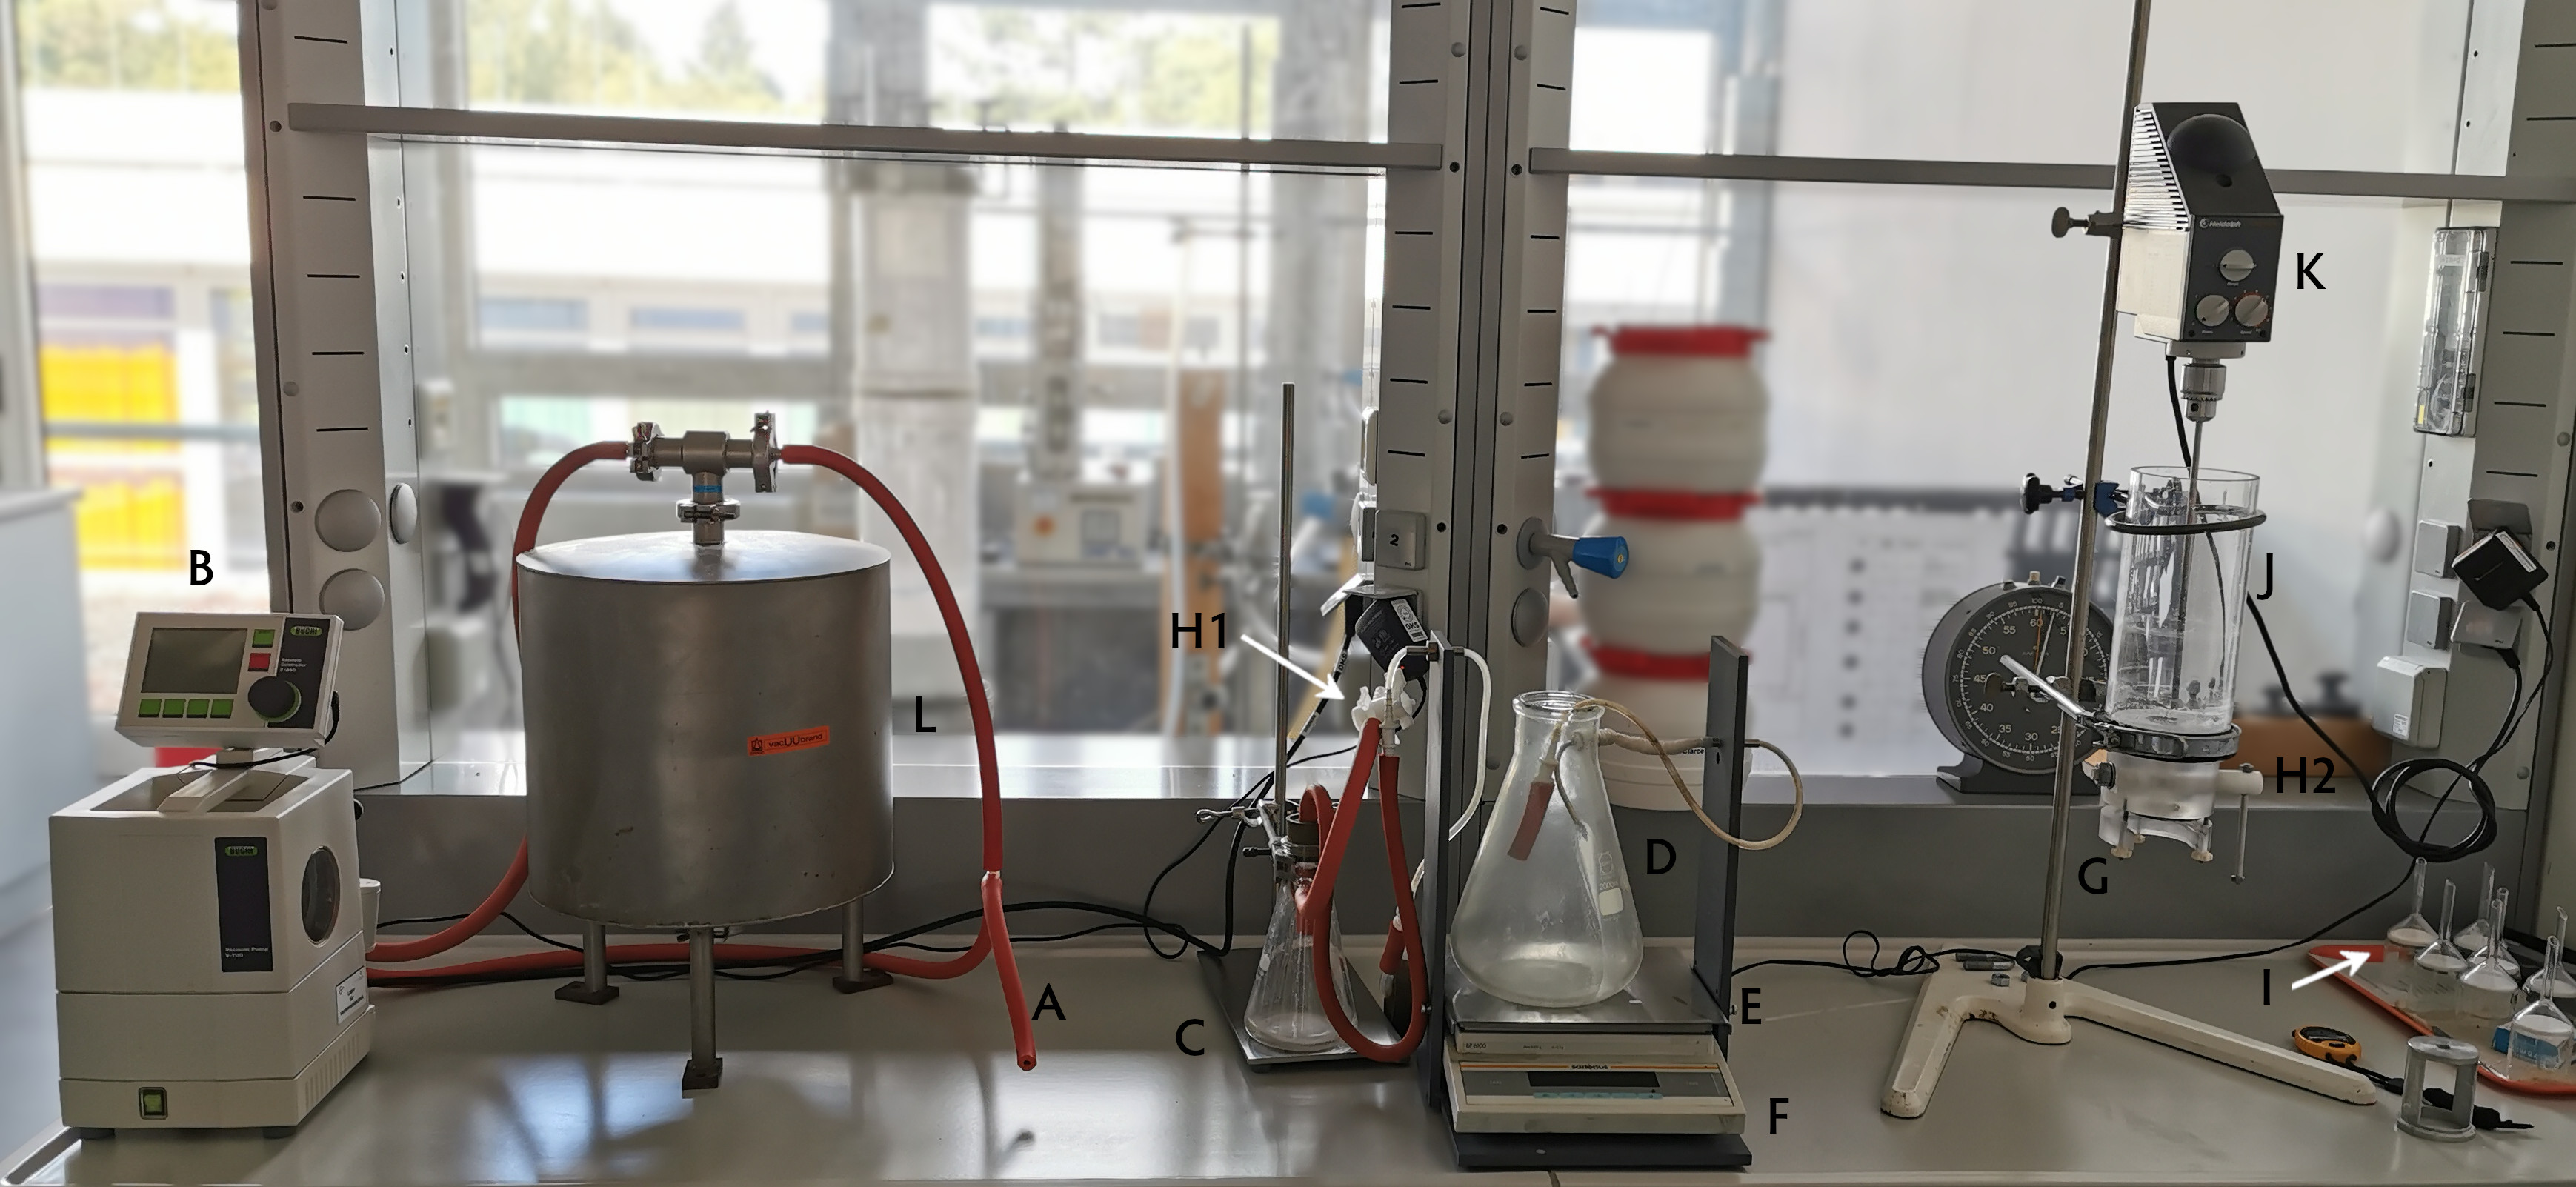
\includegraphics[width=1\textwidth]
            {Bilder/filterkuchversuchsstand.jpg} %{Bilder/LabVIEW_serialport/}
        }
    \phantomcaption
    \vspace{1em}
    \ContinuedFloat
%\captionsetup{position=bottom}
    \subfloat[Fließschema in Form einer schematischen Skizze der Filterkuchenversuchsanlage vor den Modifikationen]
    [Fließschema in Form einer schematischen Skizze der Filterkuchenversuchsanlage vor den Modifikationen \cite{Kuchenfiltration_Geweke2020} \label{fig:schema_filterkuchenversuchsstand}]{%
        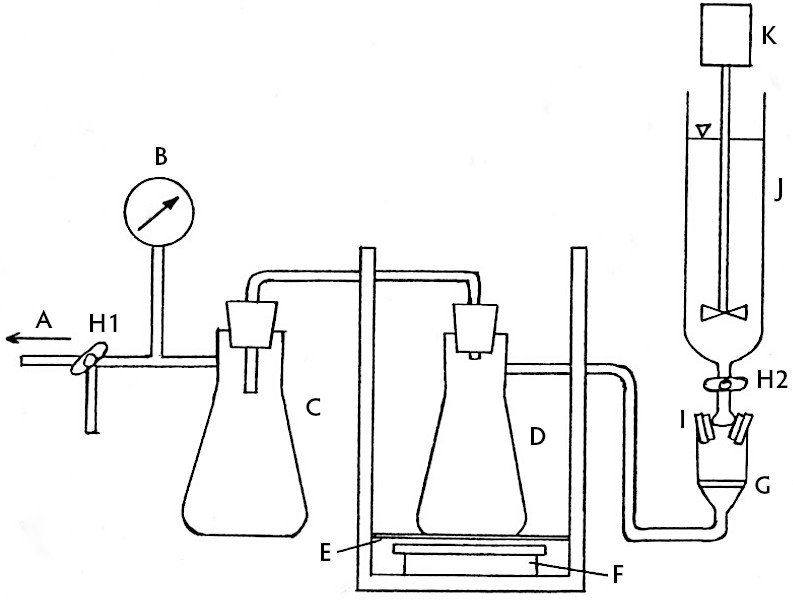
\includegraphics[width=0.75\textwidth]
        {Bilder/filterkuchversuch_schema.jpg} %{Bilder/LabVIEW_serialport/}
    }
    \caption[Filterkuchenversuchsanlage nach den Modifikationen]{Filterkuchenversuchsanlage nach den Modifikationen}
    \label{}
\end{figure}



\begin{enumerate}[label = \textbullet, itemsep = -.1em]
\item \textbf{diskret}
	\begin{enumerate}[label = --, itemsep = -.1em]
	\item a0
			\begin{enumerate}[label = -, itemsep = -.1em]
			\item die Viskosität $\eta$
			\item der Filtermittelwiderstand $\beta$
			\item die Filtrationsfläche $A$
			\end{enumerate}
	\item a1
		\begin{enumerate}[label = -, itemsep = -.1em]
		\item der Filterkuchenwiderstand $\alpha_\mathrm{V}$
		\item die Proportionalitätskonstante $\kappa$
		\item die Filtrationsfläche $A$
		\item die Viskosität $\eta$
		\end{enumerate}
	\item die Fluiddichte $\rho_\mathrm{f}$
	\item die Feststoffdichte $\rho_\mathrm{fs}$
	\end{enumerate}
	
\item \textbf{kontinuierlich}
	\begin{enumerate}[label = --, itemsep = -.1em]
	\item der irreversible Druckverlust $\Delta p_{\mathrm{konst,irr}}$
	\item das Volumen als Funktion der Zeit $V(t)=$\,\text{\Large{$\frac{m_{\mathrm{Filtrat}}(t)}{{\Large \rho_\mathrm{f}}}$}}
	\end{enumerate}

\end{enumerate}

Das Filtrationsvolumen, als Funktion der Zeit, wird über die zusammengesetzte, extensive Zustandsgröße -- der Filtratmasse $m_{\mathrm{Filtrat}}(t)$ -- bestimmt. 

\subsubsection{Sensorauswahl}

  

Im Betrieb der Filterkuchenversuchsanlage sind die Parameter, Volumenstrom $\dot{V}$ und Druck $p$, kontinuierlich zu erfassen. Die Masse des Filtrats wird von einer Laborwaage des Unternehmens Sartorius AG des Typs Practum 5101-1S detektiert. Die Waage hat eine USB Schnittstelle, die mit einem USB Kabel eine RS-232 Schnittstelle emuliert. Dafür sind, gemäß der Bedienungsanweisung der Waage, die Einstellung mit den gewünschten Schnittstellenparametern vorzunehmen. Im Rahmen dieser Arbeit werden die Schnittstellenparameter gewählt, die in der Tabelle \ref{tab:678bit_2} \textbf{schwarz} hinterlegt sind. Die Auswahl der Parameter erfolgt willkürlich. Die Übertragungsgeschwindigkeit ({\Menlo 1200 Bd}) wurde hinreichend niedrig gewählt.\\

Es haben sich zwei Drucksensortechnologien etabliert, der dehnungsresistive Drucksensor und der piezeresistive Drucksensor. Im Anhang ist eine Vergleichstabelle (siehe Tabelle \ref{fig:metall_halbleiter_dms}), die beide Sensortypen verschiedener Hersteller und deren Spezifikationen auflistet. Gemäß der Tabelle ist zu entnehmen, dass piezoresistive Sensoren kleinere Dehnungen genauer Druckdifferenzen erfassen können. Die zu erwartenden Druckdifferenzen am Versuchsstand sind gering, daher wird ein piezoresistiver Relativdrucksensor des Unternehmens B+B Thermo-Technik GmbH des Typs DRTR-AL-10V-RV1 gewählt. Der Sensor ist im verfahrenstechnischem Labor ein häufig genutztes Messinstrument und ist im Verlauf dieser Arbeit bereits vorrätig gewesen, daher findet ein finanzieller Aufwandsvergleich im Rahmen dieser Arbeit nicht statt. Die Messspanne dieses Sensors ist von -1~bis~1~bar. Die Spanne des analogen Ausgangssignals ist von 0~bis~10~V. Die technischen Daten sind der Tabelle \ref{fig:BTTG2021} im Anhang zu entnehmen. \\

\begin{table}[hpt!] %6, 7, 8 Bit Encodierung via RS-232
\caption{RS-232 Schnittstellenparameter der Practum 5101-1S Waage}
\begin{center}
\begin{tabular}{|r|c|c|c|}
\cline{2-4}
\multicolumn{1}{c|}{} &	\textcolor{black!50}{6 {\Menlo Bit}} 		&  {\Menlo 7 Bit} 		&\textcolor{black!50}{ 8 {\Menlo Bit}}\\
\hline
{\Menlo Startbit} 				& \textcolor{black!50}{1}				 & {\Menlo 1} 			& \textcolor{black!50}{1}\\ \hline
{\Menlo Symbol-/Characterbit} & \textcolor{black!50}{6} 			& {\Menlo 7} 			& \textcolor{black!50}{8}\\ \hline
{\Menlo Paritätsbit} & \multicolumn{2}{c|}{\hspace{3pt}  {\Hypatia Odd}\textcolor{black!50}{/Even/Mark/Space} \hspace{3pt}} & \textcolor{black!50}{none}  \\ \hline
{\Menlo Stoppbit}	& \textcolor{black!50}{	2} &	{\Menlo 1}& \textcolor{black!50}{0}\\
\hline
{\Menlo Baudrate} &  \multicolumn{3}{c|}{\hspace{3pt}  \,{\Menlo 1200} \hspace{3pt}}    \\ \hline
\end{tabular}
\end{center}
\label{tab:678bit_2}
\end{table}


\pagebreak
\subsubsection{Elektrotechnik der Filterkuchenversuchsanlage}

Die Sensorik ist elektrotechnisch zu verschalten, die genutzten Komponenten sind: 

\begin{itemize}
\item als Spannungsquelle ein Transformator des Typs Voltcraft TOPS-3205   
\begin{itemize}
\item Conrad Electronic AG
\end{itemize}

\item ein Drucksensor des Typs DRTR-AL-10V-RV1
\begin{itemize}
\item B+B Thermo-Technik GmbH
\end{itemize}


\item eine Laborwaage des Typs Practum 5101-1S
\begin{itemize}
\item Unternehmens Sartorius AG 
\end{itemize}

\item eine DAQ Messkarte (\textit{engl. data acquisition}) des Typs USB-6001 
\begin{itemize}
\item National Instruments (NI)
\end{itemize}
\end{itemize}



\begin{figure}[h!] %[htbp!] 
\centering
\vspace{-3em}
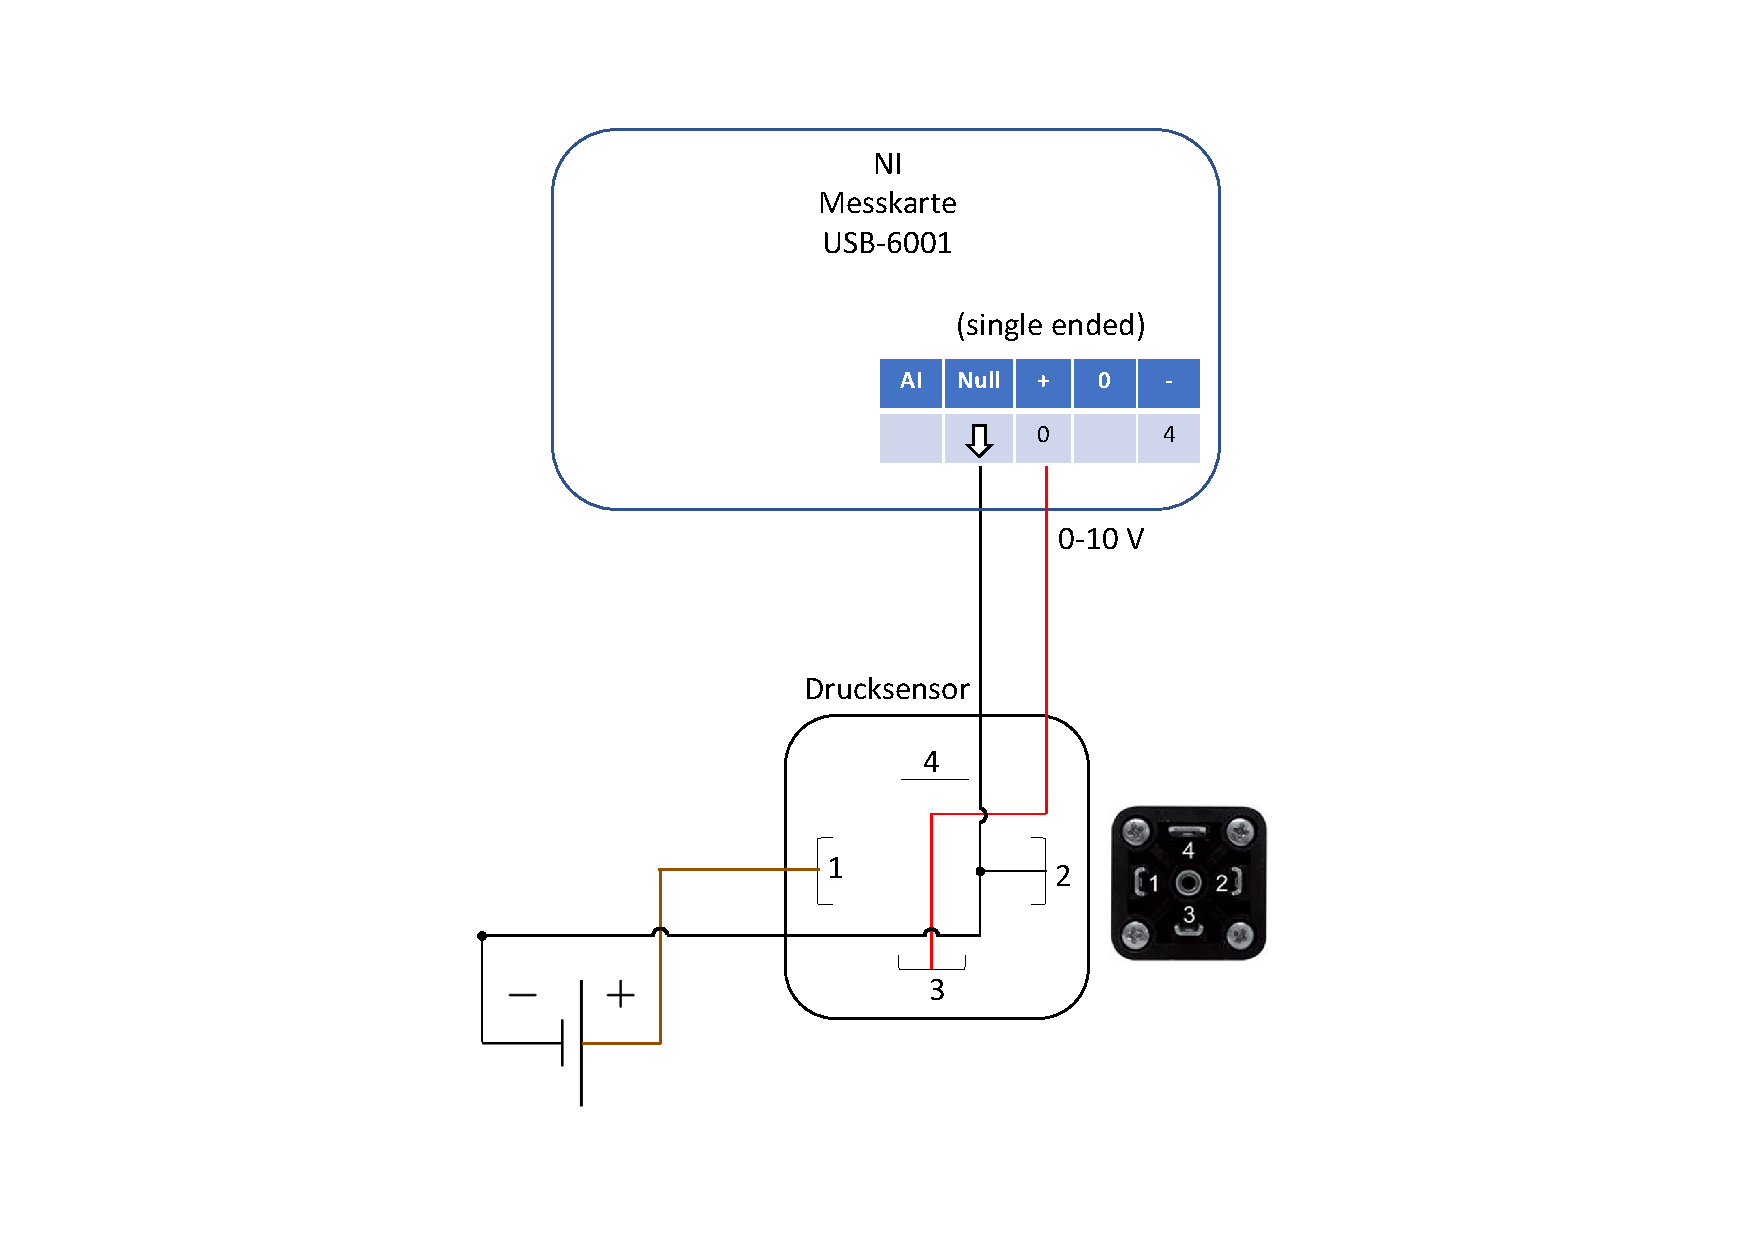
\includegraphics[width=1.02\textwidth]{Bilder/Filterkuchen_Messtechnik.pdf}
\vspace{-4em}
 \caption[]{Elektrotechnische Verschaltung der Komponenten der Filterkuchenversuchsanlage}\label{fig:filterkuchenelektrotechnik}
\end{figure}


Die Elektrotechnische Verschaltung des Drucksensors ist der Abbildung \ref{fig:filterkuchenelektrotechnik} zu entnehmen. Die Laborwaage des Typs Practum 5101-1S wird, via mitgelieferten USB-Y zu RS-232 Schnittstellenemulationsprozessorstecker Kabel, mit dem Desktop PC verbunden. 

\subsubsection{Filterkuchenversuchsanlage nach den Modifikationen}

In der Abbildung \ref{fig:filterkuchenversuchsstand_upgrade} ist die gesamte Filterkuchenversuchsanlage, nach dem Aufrüsten mit digitaler Sensorik zu erkennen. Die Grafik des Schlauchleitungs- und Gerätefließschemas ist der Abbildung  \ref{fig:schema_filterkuchenversuchsstand_upgrade} zu entnehmen. Der Versuchsaufbau wurde um eine Spannungsquelle ({\Hypatia N}) für den Drucksensor ({\Hypatia M}), einen Drucksensor ({\Hypatia M}), sowie ein Human-Machine-Interface (HMI, {\Hypatia O}) erweitert. Als HMI dient ein Desktop PC. Das Manometer zur Druckmessung bildet mit der Vacuumpumpe ({\Hypatia B}) eine Einheit. 

\subsubsection{Workflow der Filterkuchenversuchsanlagen}

In diesem Abschnitt wird der neue Workflow beschrieben. Die Datalogs werden derzeit in dem Datalogordner auf dem Desktop gespeichert. Der Tabelle \ref{tab:filterkuchenversuchsanlagenbezeichnungen} sind die Bezeichnungen der Komponenten zu entnehmen.

\begin{enumerate}
\item \textbf{{\Hypatia Starten des HMI}}
	\begin{itemize}
		\item Inbetriebnahme der Spannungsquelle
			\begin{enumerate}[label = \roman*]
			\item Hauptschalter auf der Rückseite betätigen
			\item Spannungshöhe zwischen 15 und 24 V einstellen
			\item On-button auf der Vorderseite betätigen $\Rightarrow$ Spannung stellt sich auf den gewählen Betrag ein
			\end{enumerate}	
	\item Waagensignalleitung ist mit der RS-232 Schnittstelle des HMI Towers zu verbinden.
	\item DAQ ist mit einem beliebigen USB Slot des HMI Towers zu verbinden
	\item Starten der LabVIEW Applikation \: {\Menlo Filterkuchenversuch\_V01DL.vi}
	\item Dateinamen eingeben: FK\_{\Menlo GruppenID.txt}
		\begin{enumerate}[label = -]
		\item Der Dateiname kann über den Versuchstag identisch bleiben, die Daten werden an das Datei\-ende angehängt.
		\end{enumerate}
	\item Tubidimeterdateinamen eingeben: FK\_Tubi\_{\Menlo GruppenID.txt}
		\begin{enumerate}[label = -]
		\item Der Dateiname kann über den Versuchstag identisch bleiben, die Daten werden pro Versuchsiteration überschrieben.
		\end{enumerate}
	\item Versuchseingaben tätigen
	\item wenn alle Vorbereitung der Filtrationseinrichtung \textbf{abgeschlossen} sind, dann
		\begin{enumerate}[label = \Roman*]
		\item Start des Programms: Das $\Rightarrow$ Icon oben links 
		\item öffnen des Absperrhahns H2
		\item wenn Messung abgeschlossen, dann
			\begin{enumerate}[label = --]
			\item Stop betätigen
				\begin{enumerate}[label = -]
				\item Filtratmenge bestimmen 
				\item Filterkuchendicke bestimmen 
				\item die trockene Filterkuchenmasse bestimmen
				\end{enumerate}
			\item Tubidimeter eingaben tätigen
			\item wenn abgeschlossen,  starten der nächsten Iteration bei I		 
			 \end{enumerate}
			\item \textbf{Nach der letzten Tubidimetereingabe ist das Programm nochmals zu starten und der Stop-button zu betätigen, damit die aktuellsten Tubidimeterdaten in der \newline FK\_Tubi\_{\Menlo GruppenID.txt} gespeichert werden!} 
		\end{enumerate}	
	\end{itemize}


\item \textbf{{\Hypatia Vorbereitung der Filtrationseinrichtung}}
	\begin{enumerate}[label = \alph*]
	\item Absperrhahn H1 schließen
	\item Filtrationsanlage evakuieren, dazu ist die \textit{manuell} Taste des Vakuumcontrollers zu betätigen. Bei erreichen des Solldrucks wird der isobare Zustand der Anlage erhalten.
 	\item Gereinigte Filternutsche ({\Hypatia I}) in der Kunststoffklemmvorrichtung ({\Hypatia G}) fixieren.
 	\item Es ist darauf zu achten, dass der Metallsteg der Nutschenhalterung nach vorn zeigt
	\item Absperrhahn H2 schließen (Hebelstellung: waagerecht).
	\item Schläuche sachgemäß montieren.
	\item Schutzplatte der Waage entfernen und daraufhin einschalten.	
	\item Einfüllen der Suspension und Inbetriebnahme des Rührers. 
	\item Öffnen des Dreiwegehahns H1
	\item Wenn alle Vorbereitungen abgeschlossen sind und die angezeigte Masse Konstant ist, ist die Waage zu tarieren.
	 \end{enumerate}	
\end{enumerate}

 

\begin{figure}[p!] % 
% \captionsetup{position=top}
    \centering
        \subfloat[][Filterkuchenversuchsanlage nach den Modifikationen \label{fig:filterkuchenversuchsstand_upgrade}]{%
            \hspace{0em}
            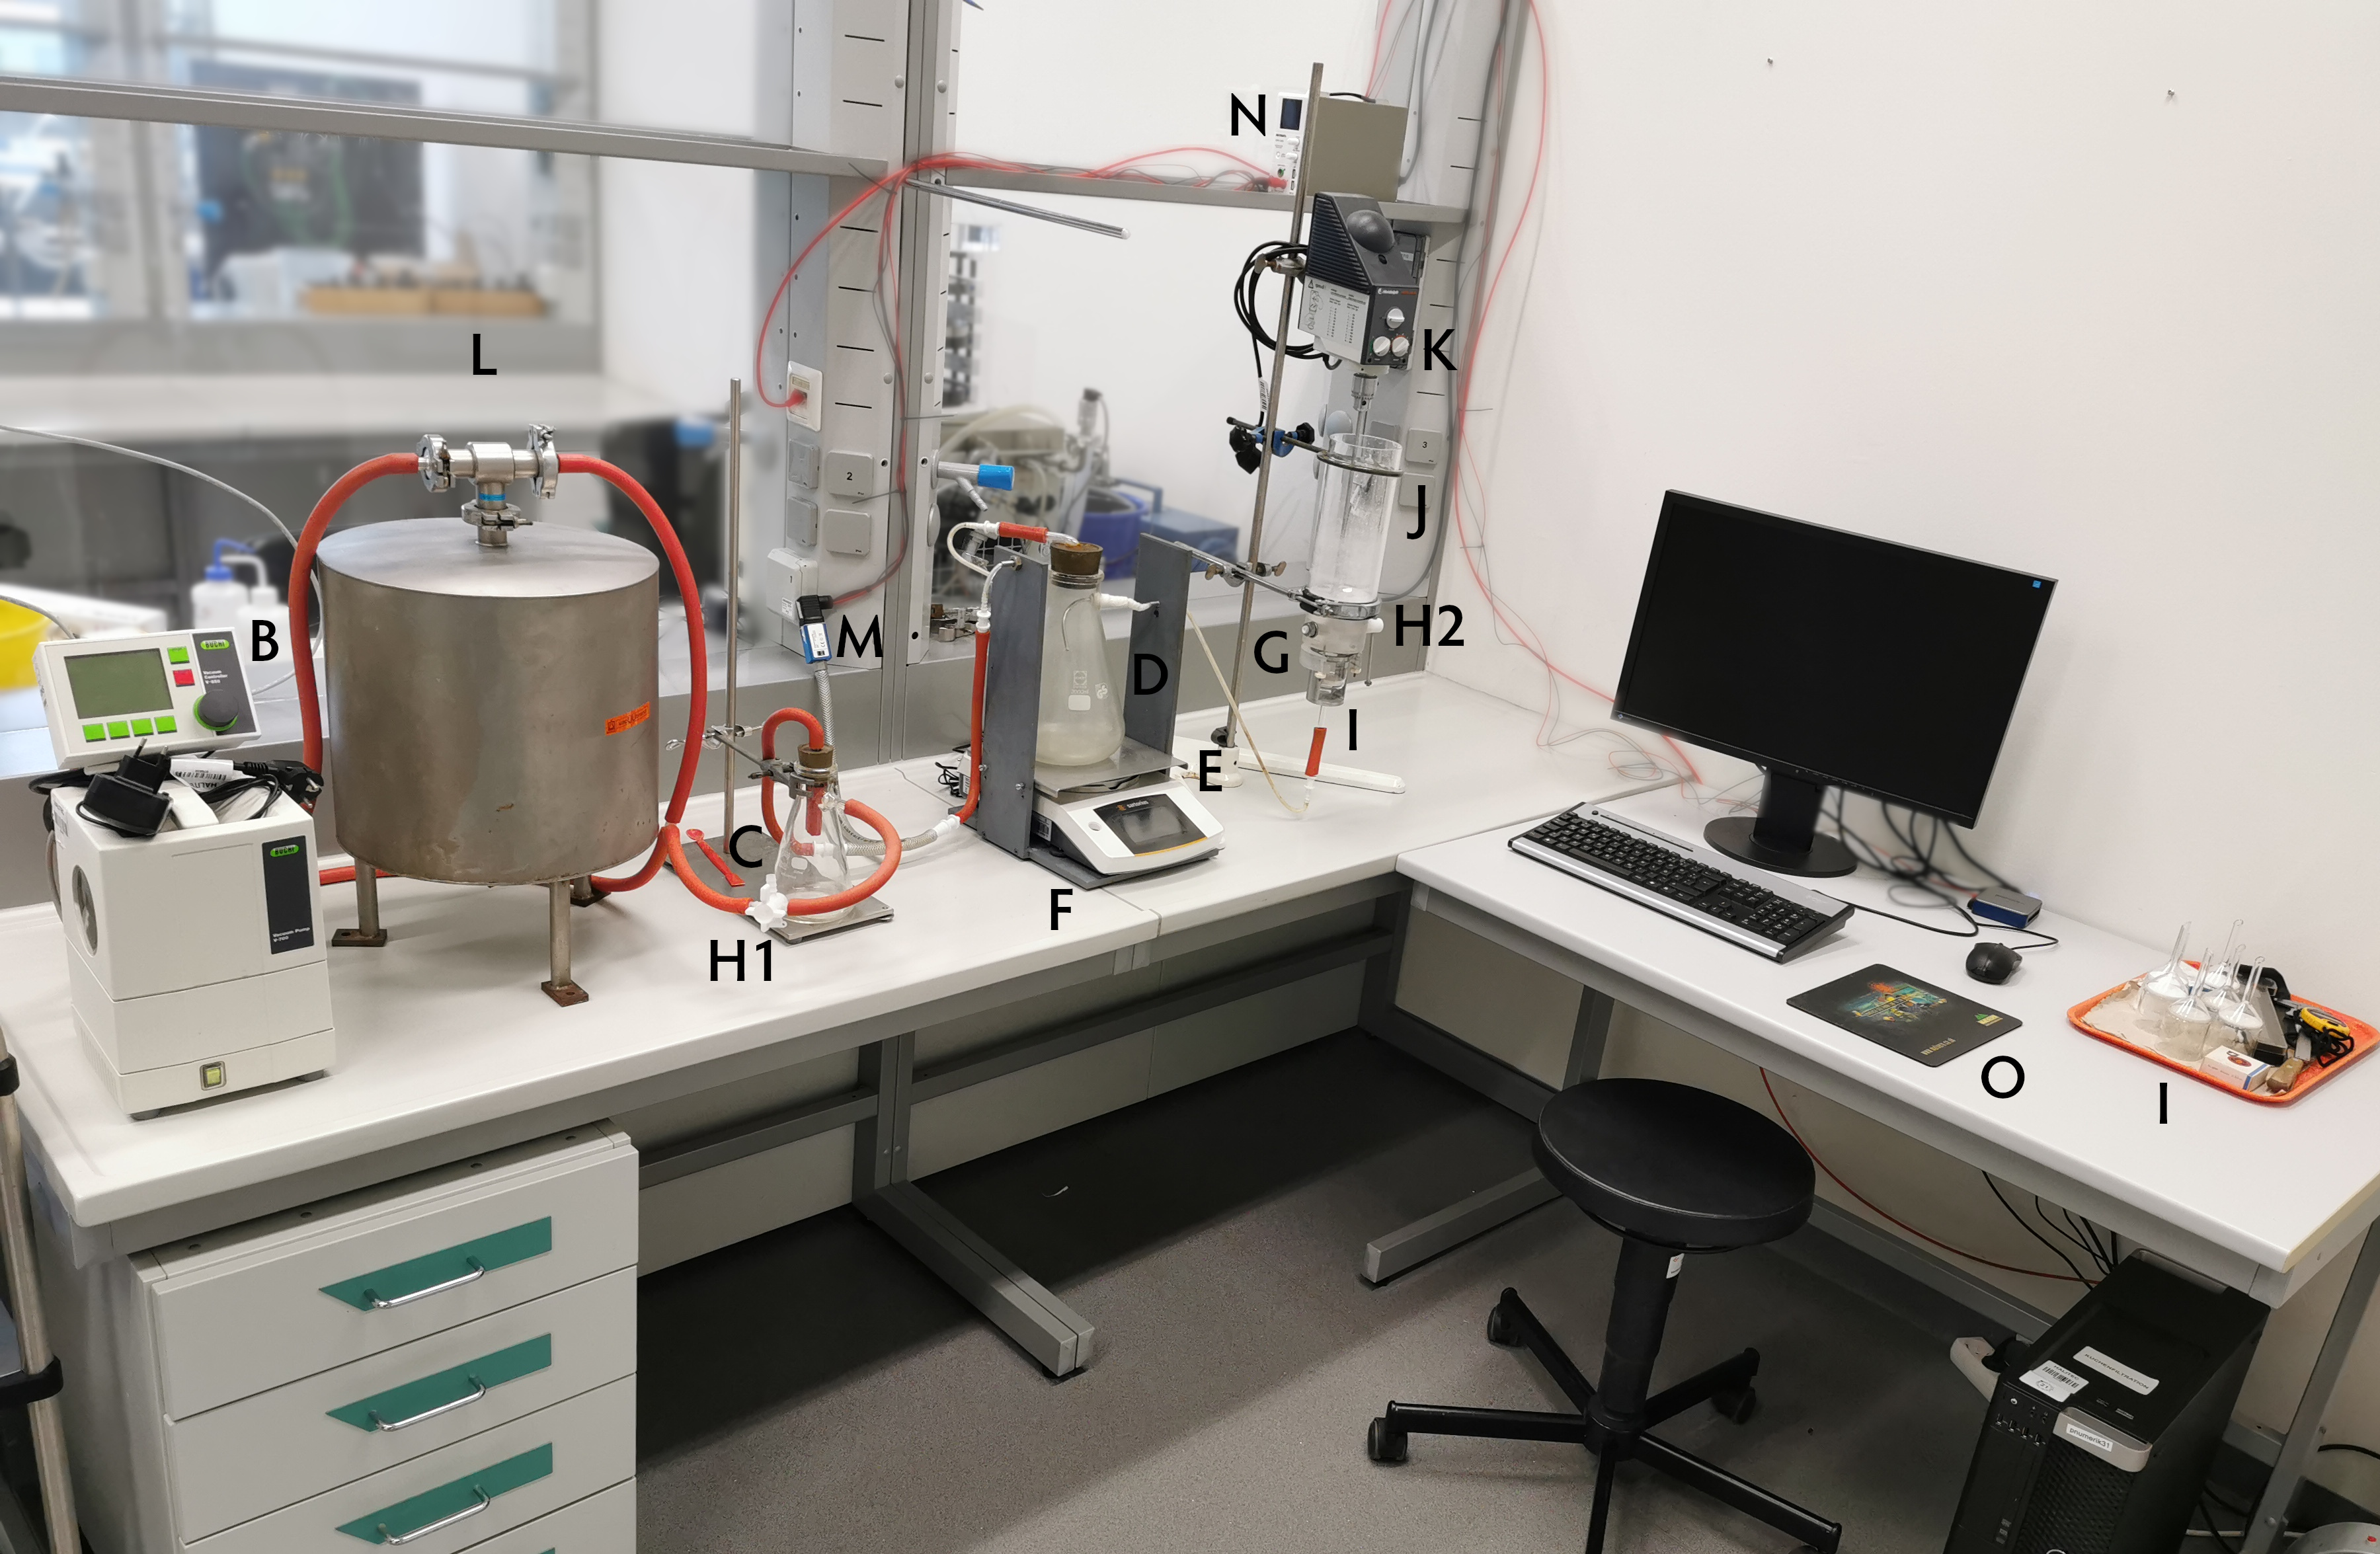
\includegraphics[width=1\textwidth]
            {Bilder/HAW/filterkuchenversuchsanlage_upgrade.jpg} %{Bilder/LabVIEW_serialport/}
        }
    \phantomcaption
    \vspace{1em}
    \ContinuedFloat
%\captionsetup{position=bottom}
    \subfloat[Fließschema in Form einer schematischen Skizze der Filterkuchenversuchsanlage nach den Modifikationen][Fließschema in Form einer schematischen Skizze der Filterkuchenversuchsanlage nach den Modifikationen \cite{Kuchenfiltration_Geweke2020} \label{fig:schema_filterkuchenversuchsstand_upgrade}]{%
        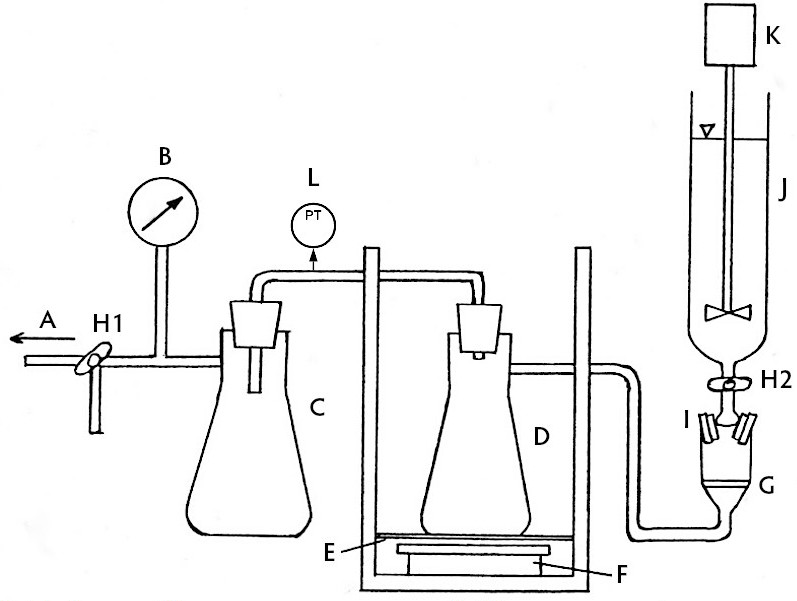
\includegraphics[width=0.65\textwidth]
        {Bilder/filterkuchversuch_schema_upgrade.jpg} %{Bilder/LabVIEW_serialport/}
    }
    \caption[]{Filterkuchenversuchsanlage nach dem Aufrüsten mit digitaler Sensorik }
    \label{fig:Filterkuchenversuchsanlage_bezeichnet_upgrade}
\end{figure}

\begin{table}[h!]
\centering
\caption{Bezeichnungen der Filterkuchenversuchsanlage}\label{tab:filterkuchenversuchsanlagenbezeichnungen}
\vspace{0.5em}
{\Hypatia \begin{tabular}{r l r l}
A & Verbindung zur Vacuumpumpe 				&  H2	& Absperrhahn	\\[0.1em]
B 	& Vacuummanometer 								& I	& Filternutsche 		\\[0.1em]  
C & Rezipient und Wasserabscheider \quad \quad	& J & Trübebehälter  \\[0.1em]
D	& Filtratauffangbehälter    							& K 	& Rührer 				\\[0.1em]	
E & Schutzplatte für Waage 							&  L & Pufferbehälter		\\[0.1em]
F 	& Waage mit digitaler Schnittstlelle 				& M & Drucksensor 		\\[0.1em]	
G & Kunststoffklemmvorrichtung									& N & Spannungsquelle \\[0.1em]	
 & --~\,Gummidichtung 									& O & HMI (Human-Machine-Interface)\\[0.1em]	
H1 &  	Dreiwegehahn									& 		& \\ 
\end{tabular}}
\end{table}



\newpage
\subsection{Wirbelschichtversuchsanlage}

Das verfahrenstechnische Labor der HAW-Hamburg Life Sciences besitzt eine Wirbelschichtversuchsanlage im Labormaßstab (siehe Abbildung \ref{fig:Wirbelschicht_mod0}). In der Abbildung \ref{fig:Wirbelschicht_konzept} ist eine Versuchsskizze des Versuchsstands dargestellt. Der gesamten Anlage ist ein Druckminderer vorgeschaltet ({\Hypatia A}). Um den Volumenstrom zu Steuern, befindet sich nach dem Druckminderer ein Handventil ({\Hypatia B}). Zur Detektion des Volumenstroms sind zwei Schwebekörperdurchflussmesser (SKDM) ({\Hypatia C}) in reihe nachgeschaltet, um einen Volumenstrom von bis zu 50~l/min Messen zu können. Mit dem SKDM auf der rechten Seite kann der Messbereich von von 0,185~bis~5~l/min gemessen werden. Mit dem SKDM auf der linken Seite sind Volumenströme 1,86~bis~50~l/min messbar. Vor dem Anströmboden muss ein Druck gemessen werden, dafür befindet sich am Boden des Fluidisierapparats ({\Hypatia E}) ein kleiner Flansch, mit dem der Druck relativ zur Umgebung mittels U-Rohr Manometer ({\Hypatia D}) gemessen werden kann. Der Fluidisierapparat besteht aus einer Plexiglassäule und dem Boden, in dem ein Gewebefilter eingespannt ist. Da Partikel mit dem Volumenstrom ausgetragen werden können, befindet sich über dem Fluidisierapparat eine Absaugung ({\Hypatia F}).

Bei diesem Versuch sind im Verlauf der Versuchsdurchführung die folgenden Parameter zu erfassen:

\begin{enumerate}[label = \textbullet, itemsep = -.1em]
\item \textbf{diskret}
	\begin{enumerate}[label = --, itemsep = -.1em]
		\item Festbettbetthöhe $h_{\mathrm{fb}}$
		\item Festbettporösität $\varepsilon_{\mathrm{fb}}$
		\item Schüttgutmasse $m_{\mathrm{Schüttgut}}$
		\item Partikeldichte $\rho_{\mathrm{fs}}$
		\item Sauterdurchmesser
	\end{enumerate}  	
	
\item \textbf{kontinuierlich}
	\begin{enumerate}[label = --, itemsep = -.1em]
		\item $\dot{V}_{\mathrm{Luft}}$ 
		\item $\Delta p (t)$ 
	\end{enumerate} 
	
\item \textbf{kontinuierlich/diskret}
	\begin{enumerate}[label = --, itemsep = -.1em]
		\item Wirbelschichthöhe $h_{\mathrm{ws}} = f(p)$
		\item Wirbelschichtporösität $\varepsilon_{\mathrm{ws}}= f(p)$ 
	\end{enumerate} 
	
\end{enumerate} 

\begin{figure}[p!] % Wirbelschichtversuchsanlage der HAW Hamburg der Fakultät Life Sciences
%\captionsetup{position=top}
\centering
     \subfloat[]
     [Wirbelschichtversuchsanlage vor den Modifikationen \label{fig:Wirbelschicht_mod0}]{%
       \hspace{0em}
       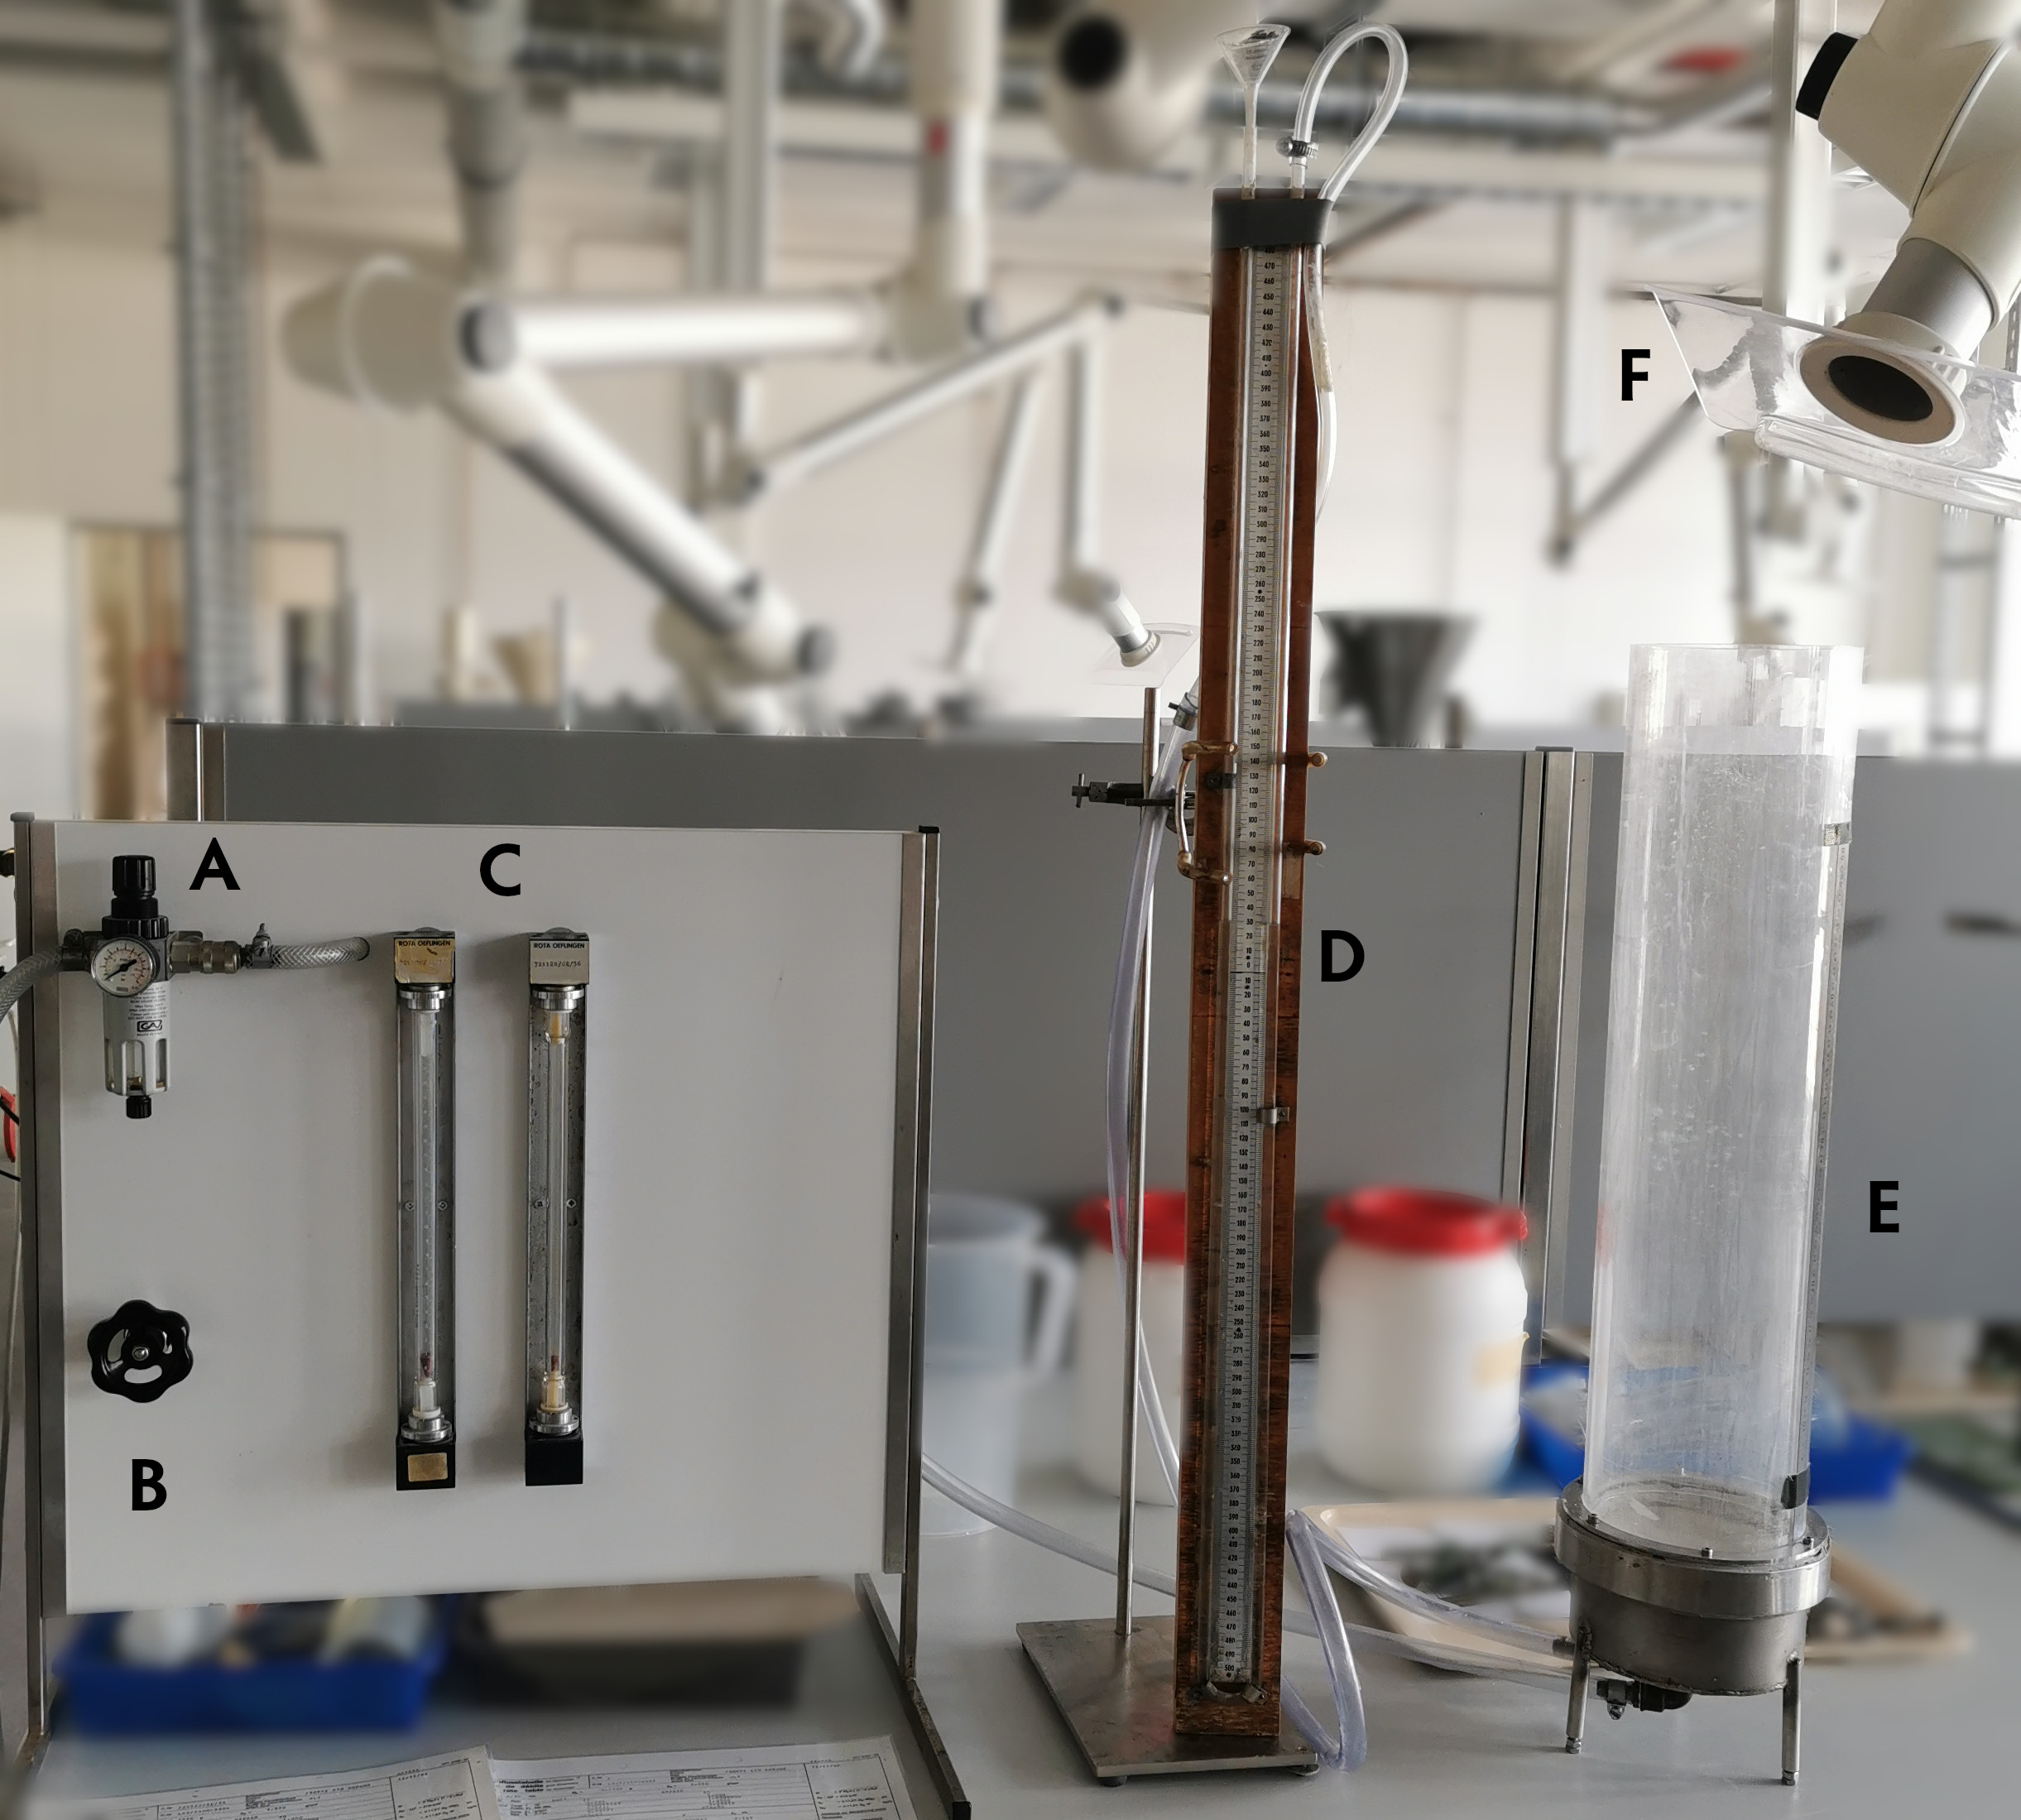
\includegraphics[width=0.8\textwidth]
       {Bilder/HAW/Wirbelschicht.jpg} %{Bilder/LabVIEW_serialport/}
     }
\phantomcaption
\vspace{1em}
\ContinuedFloat
%\captionsetup{position=bottom}
	\subfloat[][Schematische Skizze des Wirbelschichtversuchs vor den Modifikationen \label{fig:Wirbelschicht_konzept}]{%
    	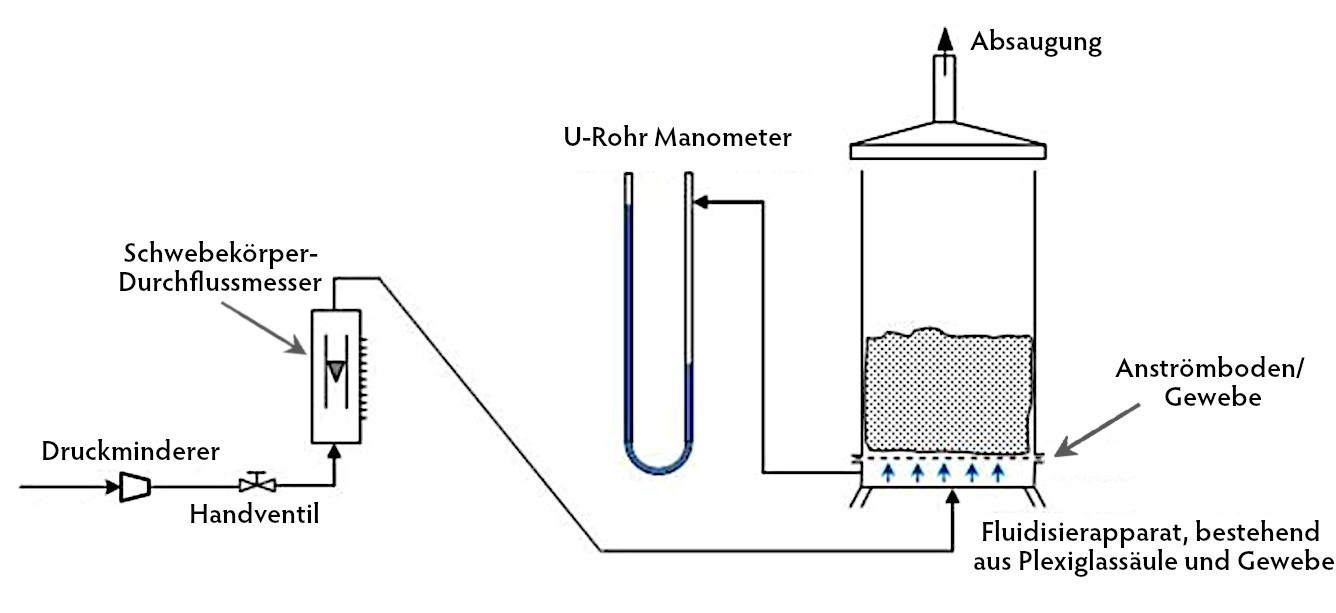
\includegraphics[width=1\textwidth]
        {Bilder/HAW/Wirbelschicht_konzept.jpg} %{Bilder/LabVIEW_serialport/}
       	}
\caption[Wirbelschichtversuchsanlage der HAW Hamburg der Fakultät Life Sciences, vor den Modifiktationen]{Wirbelschichtversuchsanlage der HAW Hamburg der Fakultät Life Sciences, vor den Modifiktationen}
\label{fig:Wirbelschicht}
\end{figure}


\newpage




Es ist hinreichend, die Wirbelschichthöhe und die daraus resultierende Porösität diskret zu erfassen. Im Rahmen dieser Arbeit wird die diskrete, manuelle Erfassung gewählt. Im Anhang befindet sich ein Diagramme für den SKDM der Messspanne von 0,185~bis~5~l/min (Abbildung \ref{fig:kleiner_skdm}) und ein Diagramm für den SKDM der Messspanne von 1,86~bis~50~l/min (siehe Abbildung \ref{fig:grosser_skdm}). Beide Diagramme enthalten Kennlinien der SKDM zzgl. jeweils zwei Approximationsfunktionen. Des Weiteren befindet sich eine Manometerkennlinie, siehe Abbildung \ref{fig:manometer_kennlinie}.\\


\subsubsection{Sensorauswahl}

Im Betrieb der Anlage sind die kontinuierlichen Parameter Volumenstrom $\dot{V}$ und Druck $p$ messtechnisch zu erfassen. Die zu erfassenen Druckdifferenzen bei diesem Versuchsstand sind ebenfalls gering, daher wird ein piezoresistiver Relativdrucksensor des Unternehmens B+B Thermo-Technik GmbH des Typs DRTR-AL-10V-RV1 gewählt. Die Messspanne dieses Sensors ist von -1~-~1~bar. Die Spanne des analogen Ausgangssignals ist von 0~-~10~V. Die Technischen Daten sind der Tabelle \ref{fig:BTTG2021} im Anhang zu entnehmen. \\

Gemäß Abschnitt \ref{sec:digi_durchfluss} sind diverse Durchflussensoren geeignet, um den Luftvolumenstrom zu erfassen. Differenzdrucksensoren sind für kleine Messbereiche nicht geeignet. Gemäß der Randbedingung des Versuchs, sind die folgenden Drucksensoren potentiell möglich.

\begin{itemize}
\item Vortexsensor
\item Drallsensor
\item Coriolissenor
\item thermischer Massendurchflussensor
\end{itemize}  

Da vor einer Kostenanalyse der Sensoren eine Anschaffung eines thermischen Massendurchflussensor des Typs VA-525 des Unternehmens CS Instruments GmbH \& Co. KG mit einer Messspanne von 0,02~-~50~l/min erfolgt ist, wird ein Vergleich der Randbedingungen und des finanziellen Aufwands im Rahmen dieser Arbeit nicht erfolgen. Das Kalibrierzertifikat des Durchflusssensors ist dem Anhang zu entnehmen (siehe Abbildung \ref{fig:va-525_kalib}). \newpage


\subsubsection{Elektrotechnik der Wirbelschichtversuchsanlage}
\label{sec:schaltung}
Die Sensorik ist elektrotechnisch zu verschalten, die genutzten Komponenten sind:

\begin{itemize}
\item als Spannungsquelle ein Transformator des Typs Voltcraft TOPS-3205   
\begin{itemize}
\item Conrad Electronic AG
\end{itemize}

\item ein Strom- Spannungswandler des Typs WAA 7-0541 
\begin{itemize}
\item Friedrich Lütze GmbH \& Co. KG
\end{itemize}

\item ein Drucksensor des Typs DRTR-AL-10V-RV1
\begin{itemize}
\item B+B Thermo-Technik GmbH
\end{itemize}

\item ein thermischer Massendurchflusssensor des Typs VA-525
\begin{itemize}
\item CS Instruments GmbH \& Co. KG
\end{itemize}

\item eine DAQ Messkarte (\textit{engl. data acquisition}) des Typs USB-6001 
\begin{itemize}
\item National Instruments (NI)
\end{itemize}
\end{itemize}

In der Abbildung \ref{fig:wirbelelektrotechnik} ist ein Schema der elektrotechnischen Verschaltung dargestellt. Der Volumenstromsensor generiert analoge Messwertsignale der Spanne 4~bis~20~mA. Die DAQ Messkarte kann analoge  Signale der Spanne 0~bis~10~V in ein digitales Signal umwandeln, daher ist zwischen dem Durchflussensor und dem DAQ ein Strom- Spannungswandler zu implementieren. Der Stromspannungswandler benötigt eine Spannungsquelle (Klemmen 1 und \textcolor{brown}{6}). Die analogen Signale des Volumenstromsensors (\textcolor{brown}{1}) und (3) werden am Stromspannungswandler an (2) und (\textcolor{black!50}{3}) angeklemmt. Die umgewandelten Signale treten aus den Klemmen (\textcolor{red}{4}) und (5) des Wandler aus. \textbf{Dieses Signal ist an einem DAQ nun differenziell zu verschalten}. Das \,{\Menlo minus} (-) Signal wird an der Messkarte demnach nicht über \,{\Menlo Null} (\textit{engl. Ground}), sondern an \,{\Menlo minus} angeklemmt. \\

Der Drucksensor generiert analoge Messsignale der Spanne 0~bis~10~V. Die Ausgänge des Sensors (2) und (\textcolor{red}{3}) sind mit \,{\Menlo Null} und \,{\Menlo plus} (+) zu verschalten. Es ist anzumerken, dass die Slots im DAQ willkürlich so gewählt wurden. Sollten die Slots gewechselt werden, dann muss es im Blockdiagramm des Hauptprogramms angepasst werden.\\


\begin{figure}[t!] %[htbp!] 
\centering
\vspace{-7em}
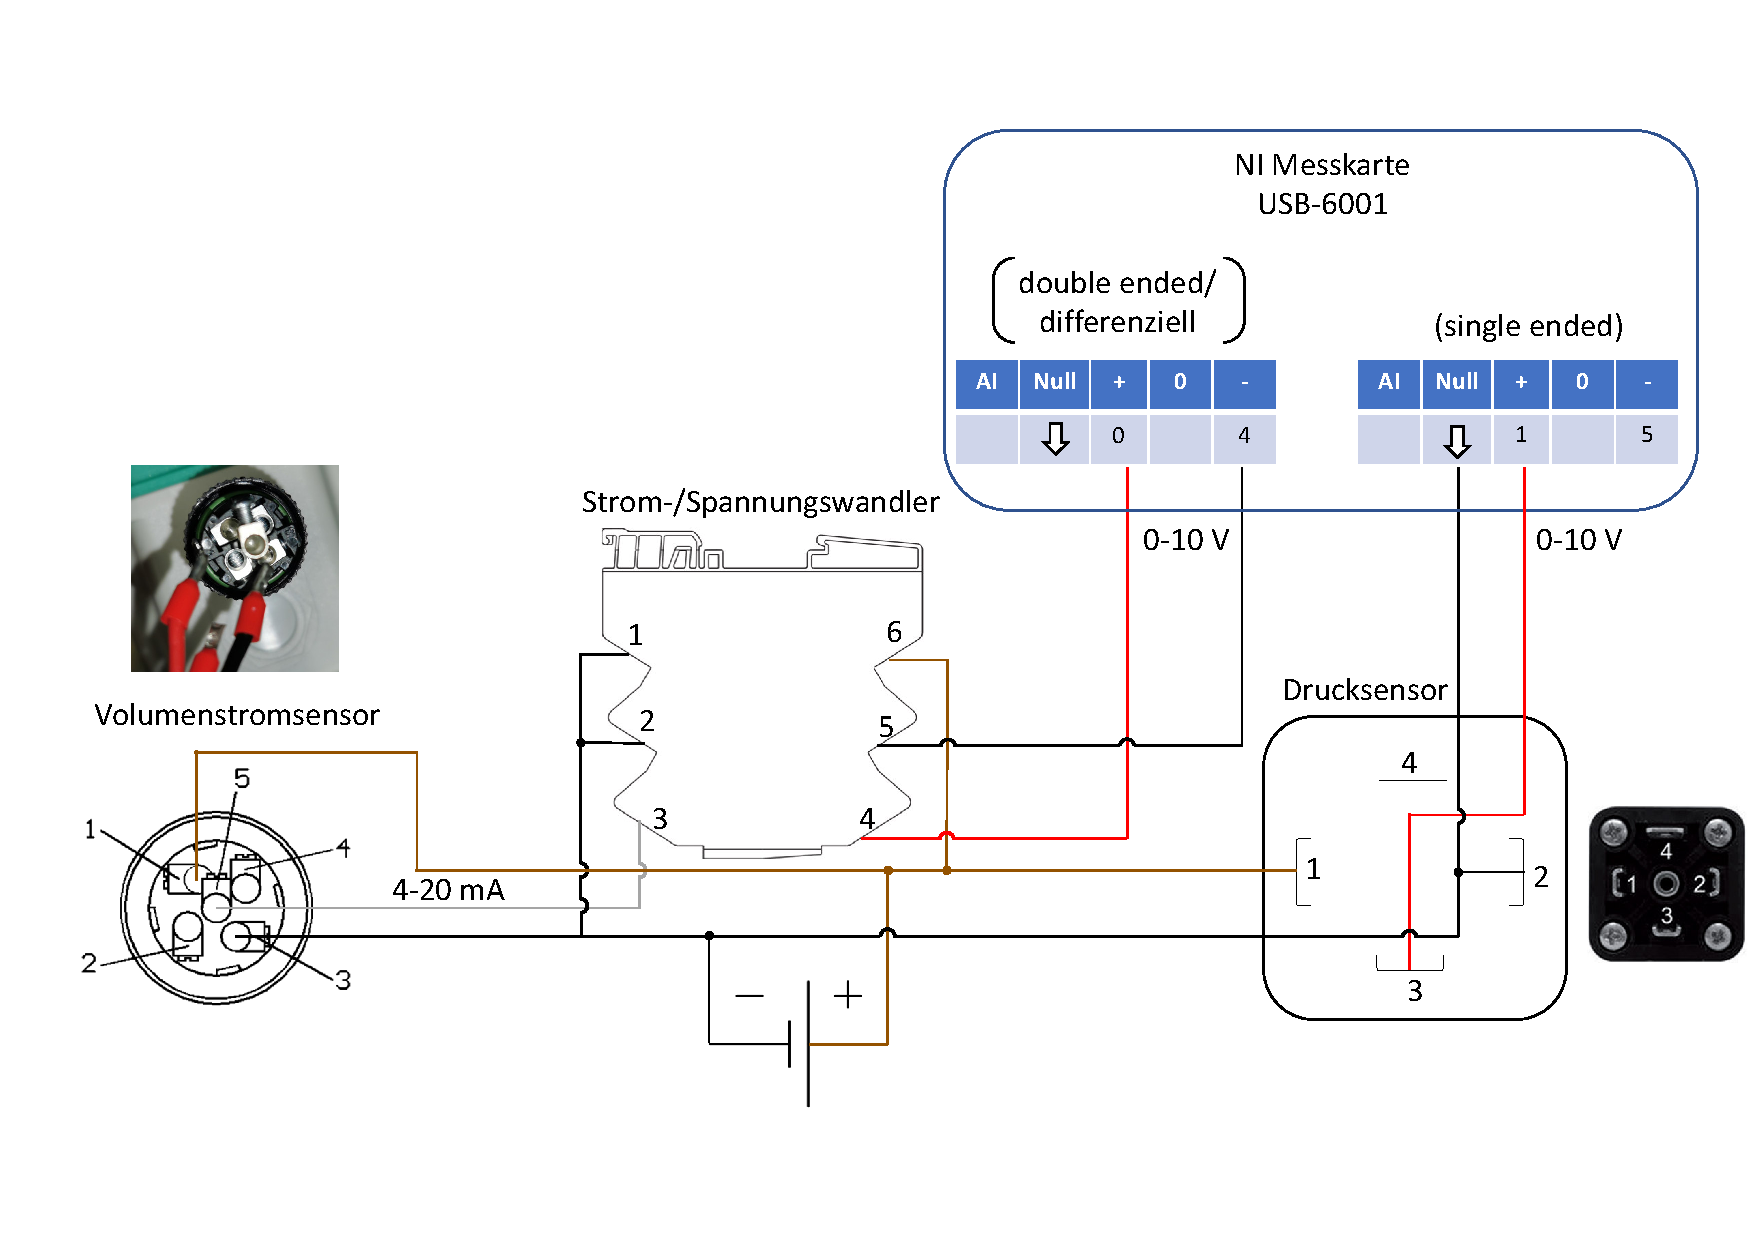
\includegraphics[width=1.02\textwidth]{Bilder/Wirbelschicht_Messtechnik.pdf}
\vspace{-4.5em}
 \caption[]{Elektrotechnische Verschaltung der Komponenten der Wirbelschichtversuchsanlage}\label{fig:wirbelelektrotechnik}
\end{figure}

\subsubsection{Wirbelschichtversuchsanlage nach den Modifikationen}

In der Abbildung \ref{fig:Wirbelschicht_upgrade} ist die Wirbelschichtversuchsanlage nach der Implementation des Druck und Volumenstromsensors zu erkennen. In der Abbildung \ref{fig:Wirbelschicht_konzept_modifiziert} ist das Fließschema der aufgerüsteten Wirbelschichtversuchsanlage abgebildet. Der Tabelle \ref{tab:bezeichnungstabelle_nach_den Modifikationen} sind die Bezeichnungen der Komponenten, der Wirbelschichtanalge nach den Modifikationen, zu entnehmen. Dem Druckminderer ({\Hypatia A}) ist das Handventil ({\Hypatia B}), zur manuellen Volumenstromsteuerung, nachgeschaltet. Nach den SKDM ({\Hypatia C}) ist der Volumenstromsensor ({\Hypatia D}) des Typs VA-525 nachgeschaltet. Nach dem Volumenstromsensor wurde ein Drucksensor ({\Hypatia E}) des Typs DRTR-AL-10V-RV1, wie auch der Volumenstromsensor, als diversitäre Redundanz implementiert. Der Drucksensor, wie auch das Manometer ({\Hypatia F}), misst den Druck vor dem Anströmboden. Über dem Fluidisertopf ({\Hypatia H}) ist eine Absaugung ({\Hypatia I}) positioniert. Wie der Abbildung  \ref{fig:Wirbelschicht_upgrade} zu entnehmen, ist es möglich eine weitere Absaugung  über dem HMI ({\Hypatia L}) zu positionieren. Des Weiteren sind weitere messtechnische Komponenten hinzugekommen. Als DAQ Messkarte wird ein Gerät des Unternehmens National Instruments des Typs USB-6001 ({\Hypatia K}) verwendet. Der Strom-/Spannungswandler ({\Hypatia G}) ist an der Trennwand befestigt. Als Spannungsversorgung für den Volumenstromsensor ({\Hypatia D}), dem Drucksensor ({\Hypatia E}), dem Strom-/Spannungswandler ({\Hypatia G}) und dem DAQ ({\Hypatia K}), wird ein Transformator ({\Hypatia \,J}) des Typs TOPS-3205 von Voltcraft verwendet.\\



\begin{table}[h!]
\caption{Bezeichnungen der Wirbelschichtversuchsanlage nach den Modifikationen} \label{tab:bezeichnungstabelle_nach_den Modifikationen}
\begin{center}
{\Hypatia \begin{tabular}{rl r l}
A & Druckminderer 						& H & Fluidisiertopf  \\[0.1em]
B & Handventil 	 							& &  --~\, Plexiglassäule\\[0.1em]
C & Schwebekörperdurchflussmesser \quad \quad 		& & -- ~\,Gewebefilter als Anströmboden  \\[0.1em]
D & thermischer Durchflusssensor 	&  I & Absaugungen \\[0.1em]
E & piezoresistiver Drucksensor	 	& J & Spannungsquelle \\[0.1em]
F & U-Rohr Manometer 					&	K & NI DAQ USB-6001 \\[0.1em]
G & Strom-/Spannungswandler	 	&  L  & HMI (Human-Machine-Interface)\\[0.1em]				
\end{tabular}}
\end{center}
\end{table}

\begin{figure}[t!] % Wirbelschichtversuchsanlage nach den Modifikationen
% \captionsetup{position=top}
    \centering
        \subfloat[Wirbelschichtversuchsanlage nach den Modifikationen]
        [Wirbelschichtversuchsanlage nach den Modifikationen \label{fig:Wirbelschicht_upgrade}]{%
            \hspace{0em}
            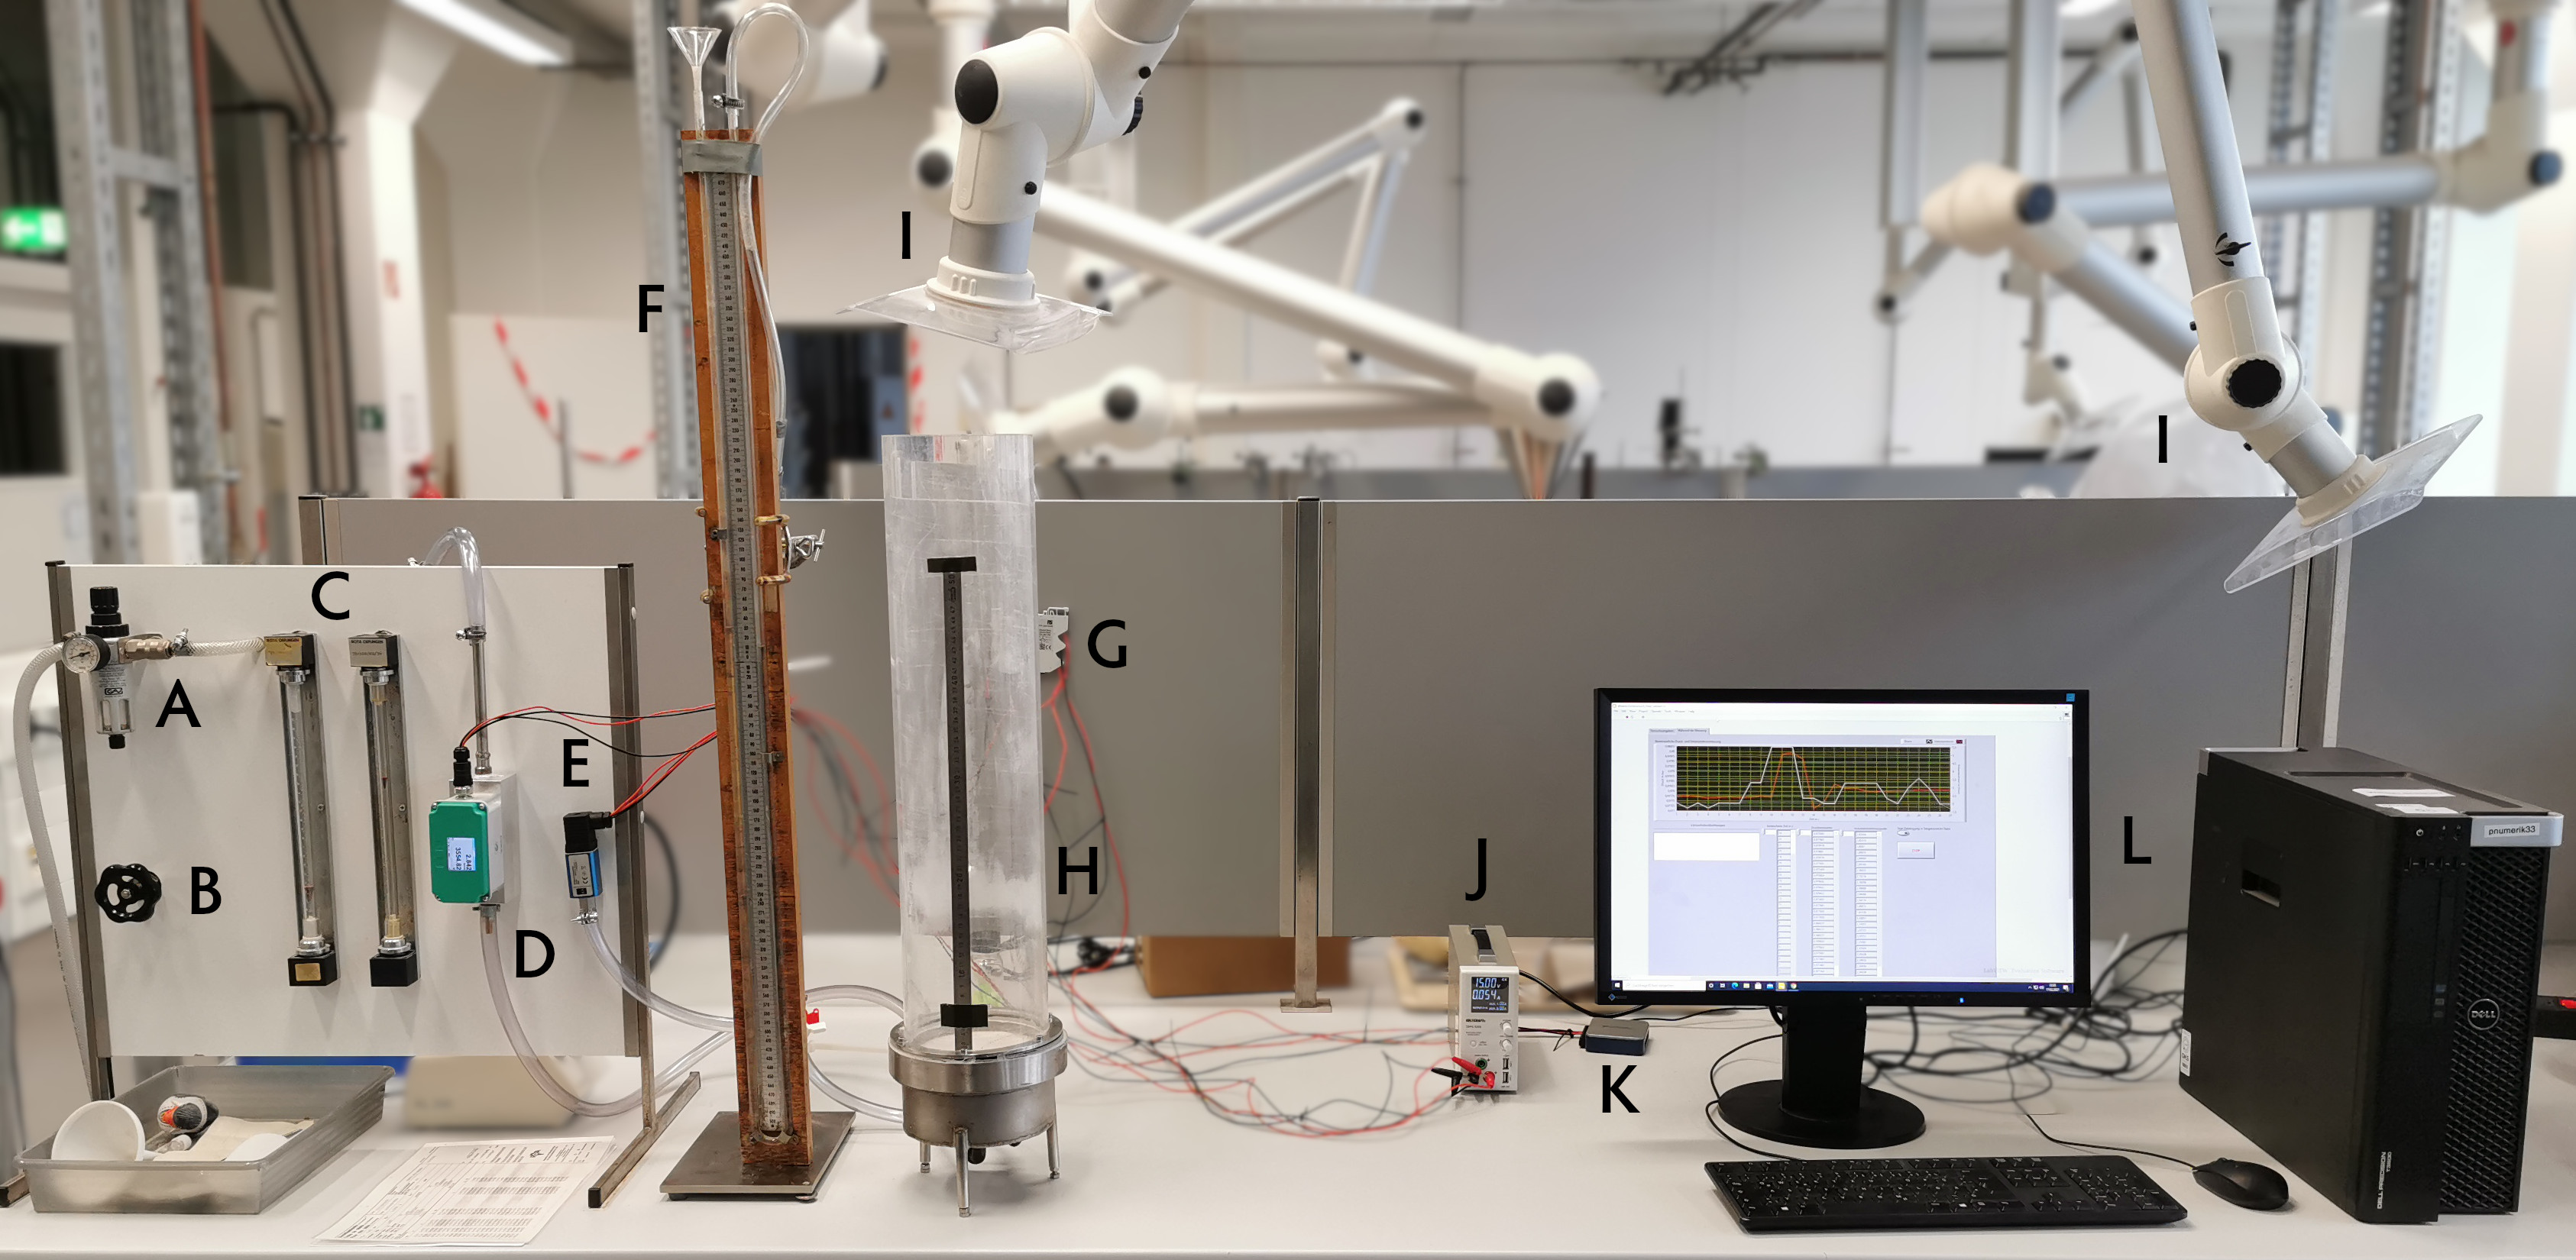
\includegraphics[width=1.05\textwidth]
            {Bilder/HAW/Wirbelschicht_upgrade.jpg} %{Bilder/LabVIEW_serialport/}
        }
    \phantomcaption
    \vspace{1em}
    \ContinuedFloat
% \captionsetup{position=bottom}
    \subfloat[][Fließschema in Form einer schematischen Skizze der Wirbelschichtversuchsanlage nach den Modifikationen \label{fig:Wirbelschicht_konzept_modifiziert}]{%
        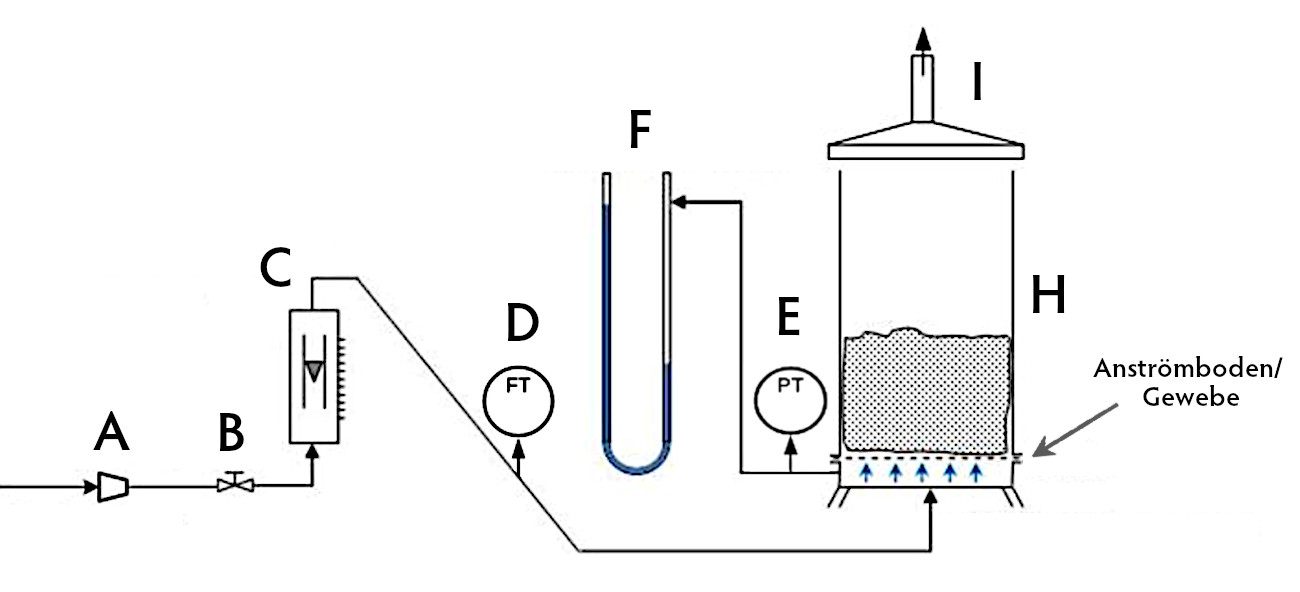
\includegraphics[width=0.8\textwidth]
        {Bilder/HAW/Wirbelschicht_konzept_modifiziert.jpg} %{Bilder/LabVIEW_serialport/}
    }
    \caption[]{Wirbelschichtversuchsanlage nach dem Aufrüsten mit digitaler Sensorik}
    \label{}
\end{figure}


\subsubsection{Workflow der Wirbelschichtanlage}

In diesem Abschnitt wird der neue Workflow der Wirbelschichtanlage beschrieben. Die Datalog-Datei wird derzeit ebenfalls in dem Datalogordner auf dem Desktop gespeichert.

\begin{enumerate}
\item \textbf{{\Hypatia Starten des HMI}}
	\begin{enumerate}[label = \Roman*, itemsep = -.1em]
		\item Inbetriebnahme der Spannungsquelle
			\begin{enumerate}[label = \roman*, itemsep = -.1em]
			\item Hauptschalter auf der Rückseite betätigen
			\item Spannungshöhe zwischen 15 und 24 V einstellen
			\item On-button auf der Vorderseite betätigen $\Rightarrow$ Spannung stellt sich auf den gewählen Betrag ein
			\end{enumerate}	
			
	\item DAQ ist mit einem beliebigen USB Slot des HMI Towers zu verbinden.
	\item Starten der LabVIEW Applikation {\Menlo Wirbelschichtversuch\_V01DL.vi}
	\item Datalognamen eingeben: WS\_{\Menlo GruppenID.txt}
	
		\begin{enumerate}[label = -, itemsep = -.1em]
		\item Der Dateiname kann über den Versuchstag identisch bleiben, die Daten werden an das Dateiende angehängt
		\end{enumerate}
	\item Versuchseingaben tätigen
	\item Start des Programms: Das $\Rightarrow$ Icon oben links 
	
\end{enumerate}
\item \textbf{{\Hypatia Praktische Versuchsdurchführung }}
\begin{itemize}
\item Druckleitung öffnen
\item Handventil zur manuellen Steuerung des Volumenstroms nutzen
\end{itemize}
\end{enumerate}

\subsubsection{Fazit}

Der Versuchsstand wurde mit geeigneter Sensorik aufgerüstet, um die kontinuierlichen Parameter, Druck $p$ und Volumenstrom $\dot{V}$, zu erfassen. Die Signale des Drucksensors sind von 0~bis~10~V und die des thermischen Massendurchflusssensors sind von 4~bis~20~mA. Eine digitale Erfassung der Festbett- bzw. Wirbelschichthöhe ist denkbar. Bei bedarf könnten bspw. geeignete optische, akustische, mechanische Entfernungsmesser, im Rahmen einer studentischen Projektarbeit, recherchiert und umgesetzt werden. Des Weiteren könnte die Steuerung des Volumenstroms, derzeit per Handventil, durch eine digitale Steuerung ersetzt werden. Der derzeitige Volumenstromsensor (VA-525) könnte entfernt und für andere Versuchsaufbauten verwendet werden.
\pagebreak


%%Schnittstellenkonfiguration_und_Signalverarbeitung_von_Messeinrichtungen,
%%Fazit,
%%Tools
%}





\begin{document} 

\begin{titlepage}
	\centering



	\begin{flushright}
		\vspace{-30em}
	
\includegraphics[width=0.55\textwidth, cfbox=CornflowerBlue!50	 2pt 0.25pt,
	 cfbox=NavyBlue!70	 3pt 0.75pt]{Bilder/HAW-Logo.png}
	\end{flushright}\par
	%\vspace{0,5cm}
%	{\scshape\LARGE HAW Hamburg \par}
\vspace{-.25em}
	\vspace{1cm}
	{\scshape\Large Masterthesis\par}
	\vspace{1.5cm}
	{\huge\bfseries Entwicklung eines Konzeptes zur Digitalisierung des Labors der
mechanischen Verfahrenstechnik der HAW, inklusive einer ersten
Teilumsetzung \par}
	\vspace{1.5cm}
	{\Large\itshape B. Sc. Daniel Ludwig Matr.: 2241272\par}
	\vfill
	\par
	\vspace{0.55cm}
	\vspace{1em}
	\begin{tabbing}
	\hspace{20pt}\=\hspace{80pt}\=\hspace{200pt}\=\kill
	\> Erstprüfer: \> Prof. Dr. Enno Stöver \\
	\> Zweitprüfer: \> Prof. Dr. Martin Geweke \\
	\end{tabbing}
	\vfill

% Bottom of the page
	{\large 28. Februar 2021\par}
\end{titlepage}
\pagebreak


%\thispagestyle{empty}
\tableofcontents
%\thispagestyle{empty}
\pagebreak


\section*{Veröffentlichungserklärung}

\manualmark \markboth{Veröffentlichungserklärung}{Veröffentlichungs- und Eidesstattlich Erklärung} 

Die vorgelegte Masterthesis mit dem Titel „Entwicklung eines Konzeptes zur Digitalisierung des Labors der
mechanischen Verfahrenstechnik der HAW, inklusive einer ersten
Teilumsetzung“ kann der Öffentlichkeit zugänglich gemacht werden.

Die Vervielfältigung und die Veröffentlichung der Masterthesis  ist grundsätzlich erlaubt.






\vspace{50pt}
\noindent\rule{5cm}{.4pt}\hfill\rule{5cm}{.4pt}\par
\noindent Datum, Ort \hfill Unterschrift

\vspace{30pt}
\noindent\rule{5cm}{.4pt}\hfill\rule{5cm}{.4pt}\par
\noindent Datum, Ort \hfill Unterschrift

\vspace{30pt}
\noindent\rule{5cm}{.4pt}\hfill\rule{5cm}{.4pt}\par
\noindent Datum, Ort \hfill Unterschrift

\vspace{30pt}




\section*{Eidesstattliche Erklärung}

Ich versichere, dass ich vorliegende Arbeit ohne fremde Hilfe selbstständig verfasst und nur die angegebenen Hilfsmittel benutzt habe. Wörtlich oder dem Sinn nach, aus anderen Werken entnommene Stellen sind unter Angabe der Quelle kenntlich gemacht. 




\vspace{50pt}
\noindent\rule{5cm}{.4pt}\hfill\rule{5cm}{.4pt}\par
\noindent Datum, Ort \hfill Unterschrift
\section*{Danksagung}

\thispagestyle{empty}

Ich möchte mich herzlich bei allen bedanken, die mich bei der Erreichung meines akademischen Ziels unterstützt haben. Allen voran selbstverständlich meine geliebte Mutter, die mir in Momenten, in denen ich aufgrund nicht offensichtlicher technischer Probleme fast verzweifelt bin oder in den Zeiten in denen ich nicht wusste wie ich neues, jedoch notwendiges neues Wissen erschließen kann, mich motiviert oder aber gezwungen hat an Tagen an denen ich 12-14 Stunden am Projekt gearbeitet habe Feierabend zu machen, naja.. bis auf die letzte Woche, hahaha. Auch mein bester Freund {\Hypatia Muhammend}, aka. {\Hypatia Mo}, war ein unheimlich wichtiger Beistand, ich Danke dir besonders!\\

Ich bedanke mich aus ganzem Herzen bei meinen Teamkollegen {\Hypatia M. Hannappel} und {\Hypatia S. Wittkowski} und den Professoren {\Hypatia C. Frank, M. Geweke, M. Hölling, A. Sievers, E. Stöver,}  die mich und meine unkonventionelle, energetische Art und Weise sowie Humor... \glqq  ertragen\grqq{}... haben. Die Welt kann ein grauer Ort sein und unsere Zeit auf Erden ist definitiv begrenzt, wenn nicht ich das weiß, wer dann. Aus diesem Grunde muss man jede Minute nutzen und zugleich genießen. Die beste Art dies zu tun ist meines Erachtens NUR durch Humor und durch die Wertschätzung jeden Moments und den Menschen in deinem Orbit, die auch nur das Beste für einen wollen.\\

Auf technischer Ebene gilt mein außerordentlicher Dank Prof. \,{\Menlo C.Frank}. Ich weiß nicht wo ich ohne Sie in Bezug auf die elektrotechnische sowie programmiertechnische Hilfe bei meinen Herausforderung wäre. Sie haben es mir ermöglicht, nach äußerst unangenehmen Startschwierigkeiten, ein Fuß in die mir noch unbekannte Welt der seriellen Schnittstellen Programmierung mit Python sowie LabVIEW zu setzen.\\

Sie alle haben mir geholfen, als mir mein Privatleben meine Arbeit erschwert hat.\\

VIELEN DANK!!!
\vspace{3em}

%\includegraphics[width=0.3\textwidth]{Bilder/DL.png}

\pagebreak
\chead{\headmark}
\automark[subsection]{section}

\addsec{Abkürzungsverzeichnis}
%\thispagestyle{empty}
%\addcontentsline{toc}{section}{Abkürzungsverzeichnis}

%Seitenzähler reset mit große römische Ziffern
%%_____________________________________________________________________
\pagenumbering{Roman}
%%_____________________________________________________________________


%\usepackage{acronym}

%\begin{acronym} 
%
%%\ac{abktag}   abkürzung wird eingeführt
%%\acs{abktag} Abkürzung wird nicht eingeführt
%%\acl{abktag} gibt die ausgeschriebene Form aus
%
%\acro{KI}[KI]{künstliche Intelligenz} 
%\acro{mvt}[mvt]{mechanische Verfahrenstechnik}
%
%\end{acronym}

% Wörter untrennbar machen:
% \mbox{Untrennbar}

\begin{large}
\begin{tabbing}
\hspace{90pt}\=\hspace{200pt}\=\kill
AI \> artificial intelligence \\
ANSI \> American National Standards Institute \\
ASCII \> American Standard Code for Information Interchange \\
Bd \> Baudrate \\
BD \> Blockdiagramm \\
BD \> Blockdiagramm \\
BuB \> Bedinung und Beobachtung \\ 
Com \> Serieller Anschluss unter Windows \\
CTS \> Clear to Send \\
DAQ \> data acquisition, Datenakquisition \\
DBMS \> Datenbank Management Systemen \\
DEE \> Datenendeinrichtung \\
DÜE \> Datenübertragungseinrichtung \\
EIA \> Electronic Industrial Alliance \\
ELN \> Electronic Laboratory Notebook \\
ERP \> Enterprise Resource Planning \\
FP \> Front Panel \\
FP \> Front Panel \\
GND \> Signal Ground \\
HMI \> Human-Machine-Interface \\
ICS \> Industrial Control System (deutsch Industrielle Kontrollsysteme) \\
IMS \> Informationsmanagementsysteme \\
IoT \> Internet of Things \\
ISA \> International Society of Automation \\
ISO \> International Organization for Standardization \\
KI \> künstliche Intelligenz \\
LIMS \> Labor Management Informations Systeme  \\
MES \> Manufacturing Excecution System\\
MESA \> Manufacturing Enterprise Solutions Association \\
MOM \> Manufacturing Operations Management\\
MVT \> mechanische Verfahrenstechnik \\
PERA \> Purdue Enterprise Reference Architecture \\
rM \> rechte Maustaste \\
RS-232 \> Recommended Standard oder Radio Section 232 \\
RTS \> Request to Send \\
RxD \> Receive Data \\
SETSVI \> Simple Elapsed Time Sub VI \\ 
SKDM \> Schwebekörperdurchflussmesser \\
SQL \> Structured Query Language \\
SSVI \> Serial Sub VI \\
TxD \> Transmit Data \\
USB \> Universal Serial Bus \\
VI \> Virtuelles Instrument \\
VT \> Verfahrenstechnik \\
WBF \> World Batch Forum\\
WSN \> Wireless Sensor Network \\
XML \> Extensible Markup Language \\
XSD \> [XML] Schema Definition \\




\end{tabbing} 
\end{large}


\pagebreak

\addsec{Symbolverzeichnis}
%\thispagestyle{empty}


\vspace{0.5em} 
\begin{large}
\begin{tabbing}
\hspace{90pt}\=\hspace{300pt}\=\kill

\textbf{Symbol} \> \textbf{Bezeichnung} \> \textbf{Einheit} \\[0.3em] 
$A$ \> Anströmfläche \> $\mathrm{m^2}$ \\
$ \vec{a}$ \> Beschleunigung \> $\mathrm{m/s^2}$\\
Bd \> Baudrate \> Byte/s  \\
$c_p$ \> Wärmekapazität \> $\mathrm{kJ / kg \cdot K}$\\
$c_w$ \> Widerstandsbeiwert \> - \\
$d$ \> Durchmesser \> $\mathrm{mm^{2}}$ \\
$\varepsilon$ \> Porösität \> - \\
$\eta$ \> dynamische Viskosität \> $\mathrm{Pa s}$ \\
$\mathit{Eu}$ \> Eulergleichung \\
$F$ \> Kraft \> $\mathrm{N}$ \\
$ \vec{F}$ \> Kraftvector \> $\mathrm{kg \cdot m/s^2}$ \\
$F$ \> Kraft \> $\mathrm{N}$ \\
$g$ \> Gravitationskonstante \>  $\mathrm{m/s^2}$\\
$I$ \> Stromstärke \>$ \mathrm{A}$ \\
$k$ \> Dehnungsempfindlichkeit \> - \\
$m$ \> Masse \> $\mathrm{kg}$ \\
$\nu$  \> Querkontraktionszahl (Poisson-Konstante) \> - \\
$P, p$ \> Druck \> $\mathrm{N/m^2}$ \\
$\psi$ \> Dehnung \> - \\
$\pi_{l,t}$ \> longitudinale/transversale Piezokonstante \> $\mathrm{Pa^{−1}}$ \\
$R$ \> elektrischer Widerstand \> $\Omega$ \\
Re \> Reynoldszahl \> - \\
$\rho$ \> Dichte \> $\mathrm{kg / m^3}$ \\
$\rho_{el}$ \> spezifischer elektrischer Widerstand \> $\Omega~ \mathrm{ \cdot~ m}$ \\
$S$ \> Surface \> $\mathrm{mm^2}$ \\
$s$ \> Filterkuchendicke \\
$\sigma_{l,t}$ \> longi./transv. mechanische Spannungskomponente \> $\mathrm{Pa}$ \\
$T$ \> Temperatur \> $\mathrm{K}$ \\
$U$ \> elektrische Spannung \> $\mathrm{V}$ \\
$\dot{V}$ \> Volumenstrom \> $\mathrm{m^2/s}$ \\
$v$ \> Geschwindigkeit, Leerrohrgeschwindigkeit \> $\mathrm{m/s}$ \\
$w$ \> charakteristische Geschwindigkeit \> $\mathrm{m/s}$ \\
$x$ \> Feinheitsmerkmal \> $\mathrm{mm}$\\


\end{tabbing} 
\end{large}

\newpage
\addsec{Indexverzeichnis}
%\thispagestyle{empty}


\vspace{0.5em} 
\begin{large}
\begin{tabbing}
\hspace{90pt}\=\hspace{200pt}\=\kill

\textbf{Index} \> \textbf{Bezeichnung} \\[0.3em] 
$\mathrm{32}$ \> Sauter(-durchmesser) \\
$\mathrm{A}$ \> Auftrieb \\
$\mathrm{a}$ \> Anström(-fläche) \\
$\mathrm{Br}$ \> Wheatstone Brücke \\
$\mathrm{c}$ \> Coriolis \\
$\mathrm{el}$ \> elektrisch \\
$\mathrm{f}$ \> Fluid \\
$\mathrm{fb}$ \> Festbett \\
$\mathrm{FM}$ \> Filtermittel \\
$\mathrm{fs}$ \> Feststoff \\
$\mathrm{G}$ \> Gravitation \\
$\mathrm{h}$ \> hydraulisch \\
$\mathrm{irr}$ \> irreversibel \\
$\mathrm{K}$ \> Filterkuchen \\
$\mathrm{konst}$ \> konstant \\
$\mathrm{L}$ \> Länge \\
$\mathrm{l}$ \> longitudinal \\
$\mathrm{m}$ \> Massen(-konzentration) \\
$\mathrm{mf}$ \> minimal Fluidisation \\
$\mathrm{Q}$ \> Querkontraktion \\
$\mathrm{s}$ \> Sink(-geschwindigkeit) \\
$\mathrm{t}$ \> transversal  \\
$\mathrm{V}$ \> Volumen \\
${\mathrm{vs}}$ \> Volumen(-konzentration) \\
$\mathrm{W, w}$ \> Widerstand \\
$\mathrm{ws}$ \> Wirbelschicht \\
$\mathrm{x}$ \> Feinheitsmerkmal \\


\end{tabbing} 
\end{large}
\pagebreak


\addsec{Glossar englischer Begriffe}


\vspace{0.5em} 
\begin{large}
\begin{tabbing}
\hspace{220pt} \=\hspace{200pt}\=\kill

\textbf{Englisch} \> \textbf{Deutsch} \\[0.3em] 
\raggedright AI \> künstliche Intelligenz \\
classification \> Klassifizieren \\
DAQ \> Datenakquisition \\
digital Twin \> digitaler Zwilling \\
dryfreezer \> Gefriertrockner \\
dustfiltration \> Staubabscheidung \\
fixed-bed \> Festbett \\
fluidization  \> Fludisierung \\
high pressure homogenizer \> Hochdruckhomogenisator \\
laser diffraction device \> Laserbeugerpartikelanalysator \\
machien learning \> maschinelles Lernen \\
particle bed, fixed-bed filtration \> Festbett-/ Kuchenfiltration \\
unit operation \> verfahrenstechnische Grundoperation \\
principal \> Auftraggeber $\Rightarrow$ Dozenten \\
rollcrusher \> Walzenbrecher \\
sieveing \> Sieben \\
standard operating procedures (SOP) \> Handlungsanweisung, Versuchsanweisung \\
supervisor \> Schichtleiter $\Rightarrow$ wissenschaftlicher Mitarbeiter \\
tensil tester \> Zugversuchapparatur \\
\end{tabbing} 
\end{large}

\pagebreak
\addsec{Tools}

 Alle Tools die im Verlauf des Projekts eingesetzt wurden sind in der folgenden Liste aufgelistet:


\begin{itemize}
\item Hardware
	\begin{itemize}
	\item Smartphone P30+ (privat) für die Fotodokumentation
	\item MacBook Pro 2011 (privat)
	\item Windows 10 Desktop PC (privat)
	\item Windows 10 Desktop PC
	\end{itemize}

\item Software
	\begin{itemize}
	\item Powerpoint für Präsentation, Grafikerstellung (z.B. elektrisches Schaltschema, Datenbank) und Bildmanipulationen.
	\item PDF24 
		\begin{itemize}	
		\item zum beschneiden der PDF Ränder
		\item Zum "Drucken" von Dateien in ein PDF, anstelle eines Papiers
		\end{itemize}
	\item Tabellenkalkulationsprogramm: Excel
	\item Bildmanipulation: GIMP 
	\item Textsatz: \LaTeX zur Anfertigung des Dokuments
		\begin{itemize}
		\item[-] Fonts (XeLaTeX notwendig, um die Fonts nutzen zu können)
			\begin{itemize}			
			\item[1] Arno Pro
			\item[{\Hypatia 2}] {\Hypatia Hypatia Sans}
			\item[{\Menlo 3}] {\Menlo Menlo (Python font)}
			\end{itemize}
		\item[-] Bibliotheksmanagement: JabRef 
		\item Für Formeln im Hauptdokument wurden die folgenden Normen beachtet:
		\begin{itemize}
		\item DIN 1338 Formelschreibweise und Formelsatz
		\item DIN 1304 Formelzeichen
		\item DIN 1301 Einheitennamen, Einheitenzeichen
		\item DIN 1313 Größen 
		\end{itemize}		
		\end{itemize}
	\item LabVIEW 2019 auf den HMI`s an der HAW Life Sciences	
	\item LabVIEW 2020 auf dem MacBook pro und dem privatem PC
	\item LabVIEW 2021 auf den HMI`s an der HAW Life Sciences
	\item Anaconda als Python Distribution
		\begin{itemize}
		\item Spyder als Python Editor
		\end{itemize}
\end{itemize}
\end{itemize}


%\section*{Abstract}
\pagestyle{scrheadings}
%Seitenzähler reset mit arabischen Ziffern
%%_____________________________________________________________________
%\pagenumbering{arabic}
%
% oder
%
%\setcounter{page}{1}
\markboth{Abstract}{Zusammenfassung/Abstract}


\begin{abstract}
Im Verlauf des Projekts wurden Konzepte zur Digitalisierung des verfahrenstechnischen Labors erstellt. Es sind zwei Konzepte erstellt worden, die aufeinander aufbauen. Das erste Konzept mit dem Titel \glqq Konzept 3.0\grqq{} beschreibt die Generierung von Messwertdaten mittels Sensoren und die softwaretechnische Verarbeitung und Archivierung. Das zweite Konzept, mit dem Titel \glqq Konzept 4.0\grqq{} beschreibt die zukünftige, potentielle Implementierung weitere Applikationen im Rahmen von Big Data. Da das zweite Konzept Datenbankmanagementsysteme im Zentrum hat, ist ein Datenbankkonzept, angelehnt an den ISA-S95 and B2MML, erstellt und dieses anschließend auf ein relationales Datenbankkonzept transferiert worden. Abschließend wurden zwei Versuchsstände, die Wirbelschichtversuchsanlage und die Filterkuchenversuchsanlage, mit digitaler Sensorik ausgestattet und Programme in LabVIEW geschrieben, die die Datenströme beider Versuchsstände verarbeiten können und Tabstoppgetrennte \,{\Menlo *.txt}-Dateien generieren.
\end{abstract}


\vspace{2em}


\selectlanguage{english}


\begin{abstract}
In the course of the project, concepts for digitizing the process engineering laboratory were created. Two concepts have been created. The second one build on top of the first one. The first concept, entitled Concept 3.0, describes the generation of measured value data by means of sensors and the software processing and storage. The second concept, titled Concept 4.0, describes the future, potential implementation of further applications in the context of Big Data. Since the second concept has database management systems at its core, a database concept, based on ISA-S95 and B2MML, has been created and then transferred to a relational database concept. Finally two test rigs, the fluidization bed test rig and the filtration (fixed-bed) test rig, have been equipped with digital sensors. Programs have been written in LabVIEW that can process the data streams of both test rigs and generate tab-stop separated \,{\Menlo *.txt} files.
\end{abstract}

\selectlanguage{ngerman}
\pagebreak

\automark[subsection]{section}
\pagenumbering{arabic}
\section{Einleitung}

%Ende des Jahres 2019 hat sich eine Herausforderung angebahnt, mit der die gesamte Menschheit nicht gerechnet hat. Das folge Jahr 2020 wurde maßgeblich von der Herausforderung, die Bewältigung der Covid-19 Pandemie geprägt. Die globale Marktwirtschaft, Infrastrukturen und vieles mehr wurden auf die Probe gestellt. Systeme die sich über Jahrzehnte etabliert und bewährt haben wurden ins wanken gebracht. Systeme wie unter anderem das Bildungssystem. Dieser Umstand hat neben der bereits fortschreitenden Digitalisierung, sei es im Privatsektor als auch in der Industrie als weiterer Treiber fungiert, die Digitalisierungsgeschwindigkeit zu erhöhen. Im Jahr 2011 wurde für die digitale Transformation in der Industrie der Name Industrie 4.0 in Umlauf gebracht.\\

Die Digitalisierung in der Wirtschaft hat im Jahre 2020 Dimensionen erreicht, dass Forscher mittels \glqq Supercomputern\grqq{} und \textit{\textbf{k}ünstlicher \textbf{I}ntelligenz} (KI) beispielsweise chemische Verbindungen für die Reifenherstellung oder Enzymformulierung errechnen, mit der die Ethanolproduktion optimiert werden kann \cite{lab40}. Mittels \textit{Digitaler Zwilling}, im englischen \textit{digital Twin}, können Produkte, Produktionsabläufe oder ein gesamter Prozess, durch die Kopplung von Produktions- und Produkt Twin, abgebildet und somit optimiert werden. Mittels Digital Twins lassen sich sogenannte Soft-Sensoren integrieren (angewandte numerische Simulation). In Produktionsprozessabschnitten, in denen die Bedingungen es nicht erlauben einen realen Langzeitsensor zu implementieren, können, mittels Digital Twins, Sensoren in Simulationssoftware generiert werden, die mit einem Prozess synchronisiert sind, um Totzeiten zu verringern oder zu eliminieren, bis schlechte Produktionsbedingungen detektiert werden können. Dadurch kann die Effizienz eines Prozesses signifikant gesteigert werden \cite{digitwin_prozessmodellierung}. \\ 

Abhängig vom Kontinent, Staat, Region und Branche wird der digitale Wandel anders wahrgenommen. Eine Einteilung nach Kondratjew ist nicht Eindeutig, dennoch erfüllt der digitale Wandel gemäß \cite{digitale_trans_kondratjew} alle Kriterien, um den Platz des 6. Kondratjew-Zyklus einzunehmen. Im Privatsektor nimmt die Zahl an \glqq smarten\grqq{} Geräten stetig zu. Das ein Smartphone mit einem Smart TV autonom kommuniziert ist bereits gelebter Alltag. Auch in der Industrie kommunizieren Sensoren, Geräte, Maschinen, Aggregate bereits autonom untereinander, aber auch mit \textbf{E}nterprise \textbf{R}esource \textbf{P}lanning (ERP)-, \textbf{M}anufacturing \textbf{E}xcecution \textbf{S}ystemen (MES) oder \textit{\textbf{M}anufacturing \textbf{O}perations \textbf{M}anagement} (MOM) und ähnlichem. Smarte Sensoren sind im Stande, bei autonomer Erkennung einer Erhöhung der Standardabweichung sich selbst zu kalibrieren \cite{smarte_sensoren}.\\

Es lässt sich erahnen, dass sich die Datenmengen pro Zeiteinheit, Prozess o.ä. die nächsten Jahre stetig erhöhen wird. Nun sind Konzepte gefragt, wie sich die \textbf{\glqq relevanten\grqq{}} Daten intelligent archivieren lassen, um sie in Echtzeit oder zu einem späteren Zeitpunkt verhältnismäßig einfach verarbeiten und auswerten zu können, um beispielsweise Produktionsprozesse zu optimieren. \\

Damit zukünftige Absolventen der HAW diesen Anforderungen schneller gerecht werden können, ist das erste Ziel dieser Arbeit, den Status quo des verfahrenstechnischen Labors zu erfassen, um die nächsten Schritte einzuleiten, damit der Stand der Technik in der Industrie noch besser approximiert werden kann.

%Die Zielsetzung dieser Arbeit ist nun, ein ganzheitliches Digitalisierungskonzept für das  Verfahrenstechnische Labor an der HAW- Hamburg Life Science, Standort Bergedorf, zu konzipieren, um Studierende einerseits optimal auf das operative Geschäft in der privat Wirtschaft vorzubereiten und andererseits das operative Geschäft, in Bezug auf Labor Untersuchungen, Datenverwaltungsschemas

\subsection{Ist-Analyse des Verfahrenstechnik Labors}

In der Verfahrenstechnik gibt es für die unterschiedlichsten verfahrenstechnischen Operationen (Unit Operations), wie z.B. das Trennen von Stoffgemischen oder das Zerkleinern von Partikeln, verschiedene Versuchsstände. Um sich einen Überblick über das \textbf{v}erfahrens\textbf{t}echnische (VT) Labor zu machen, kann das Labor auf mindestens drei unterschiedliche Weisen betrachtet werden. 

\begin{enumerate}[leftmargin = 1.2em]
\item Das VT-Labor kann in die \textbf{Unit Operations}, mit den Versuchsständen und den jeweiligen Komponenten wie Apparate, Messtechnik und Datenverarbeitung, unterteilt werden. Diese Sichtweise eignet sich besonders, um sich einen Überblick zu verschaffen.

\item Betrachtet man das VT-Labor unter dem Aspekt der \textbf{anfallenden Daten} (siehe Tabelle \ref{tab:Versuchsparameter} im Anhang), die bei den Versuchsständen generiert werden, dann kann das VT-Labor in diskrete und kontinuierlich anfallende Daten unterteilt werden. Folglich sind im Rahmen einer Datenverarbeitung mindestens zwei Lösungsansätze notwendig. 

\item Eine differenzierte Betrachtung der anfallenden Daten führt zur nächsten Klassifizierung, die Einteilung nach  \textbf{Messaufgabe}. Verfahrenstechnische Messaufgaben könnten die folgenden sein:


\begin{enumerate}[label = \textbullet , itemsep = -0.1em]
	\item Volumenstrom-/Massenstrommessung (kontinuierlich)
	\item Temperaturmessung (kontinuierlich/diskret)
	\item Wiegen (kontinuierlich/diskret)
	\item Druckmessung (kontinuierlich/diskret)
	\item Konzentrationsmessung (kontinuierlich/diskret)
		\begin{enumerate}[label = - , itemsep = -0.25em]
			\item Luftfeuchtebestimmung (diskret/kontinuierlich)
			\item Feuchtebestimmung von Feststoffen (diskret)
			\item pH-Wert Messung (kontinuierlich/diskret)
			\item Gaskonzentrationsmessung (kontinuierlich)
		\end{enumerate}
\end{enumerate}
\end{enumerate}

\begin{table}[hp!] % Mechanische Unit Operations, deren Versuchsstände und Messtechnische Einrichtungen
\caption{Mechanische Unit Operations, deren Versuchsstände und messtechnische \\Einrichtungen}
\centering \vspace{5pt}
{\fontsize{11}{13,2}
\begin{NiceTabular}{Wc{2,5cm}Wc{2cm}rl}[hvlines, 
code-before = \rectanglecolor{blue!13}{19-1}{31-4}, 
code-before = \rectanglecolor{red!12}{6-2}{8-4}]
\Block{1-2}{\textbf{Unit Operations}} &						&  \textbf{Versuchsstände} & \textbf{digitale Schnittstelle} \\
\hline
\Block{7-1}{ Trennen}	& \Block{1-1}{Klassieren} & Sichten				 & keine \\

								&  \Block{3-1}{Filtration}	& \hatchcell[gray!50] Kuchenfiltration	& keine\\
								&									& Blaine 										& keine \\
								&									& Staubabscheidung						& \textcolor{OliveGreen}{\textbf{USB}} \\
								& \Block{3-1}{thermisch} & Gefriertrocknen 							&  \textcolor{OliveGreen}{\textbf{USB}} \\
								& 									& Trocknungsofen 							&  \textcolor{OliveGreen}{\textbf{USB, LAN}} \\
								&									& Vakuumtrockner 							& keine \\								
\Block{1-2}{Fluidisieren} &								& \hatchcell[gray!50] Wirbelschicht & keine \\
\Block{6-2}{ Partikelzerkleinerung} &					& Backenbrecher & keine \\
								& 									&	Planetenkugelmühle 	&  \textcolor{OliveGreen}{\textbf{RS-232, RS-485}} \\
								&									& Prallmühle					& keine \\
								&									& Walzenmühle			 	& keine \\
								&									& Schneidmühle		 		& keine \\
								&									& Hochdruckhomogenisator 	& keine \\
\Block{3-2}{ Mischen} 	%&									&	Feststoffdispergierer	& keine	\\	
								&									& Intensivmischer	& \textcolor{OliveGreen}{\textbf{USB}} \\
								&									& Conchiermaschine	& keine \\
								&									& Rührversuch 	& \textcolor{OliveGreen}{\textbf{RS-232}} \\	
\hline \Block{11-1}{} & \Block{6-1}{MVT}			& Zugversuch    & 	 \textcolor{OliveGreen}{\textbf{RS-232}} \\
								&									& Siebturmanalyse 				& keine \\
								& 									& Luftstrahlsiebung &\textcolor{OliveGreen}{\textbf{RS-232, USB}} \\
								&									& Scherzelle 	& \textcolor{OliveGreen}{\textbf{RS-232}} \\
								&									& Stampfdichte 	& keine \\
								&									& Laserbeugungs-Partikelgrößenanalyse 	& \textcolor{OliveGreen}{\textbf{USB}} \\								
\Block{3-2}{Analyseeinrichtungen}								&									& Waagen 		& \textcolor{OliveGreen}{\textbf{USB}} \\
\Block{6-2}{}				&									& IR-Waagen 	& \textcolor{OliveGreen}{\textbf{RS-232}} \\
								&									& Refractometer	& \textcolor{OliveGreen}{\textbf{RS-232}} \\
								&									& Fluiddichtemesser 	& \textcolor{OliveGreen}{\textbf{RS-232}} \\
								&									& Gaspyknometer 	& \textcolor{OliveGreen}{\textbf{RS-232}} \\
								&									& Mikroskope 	& \textcolor{OliveGreen}{\textbf{USB}} \\		
								&									& Viskosimeter &	\textcolor{OliveGreen}{\textbf{USB}} \\	

\end{NiceTabular}
}
\label{tab:unitoperations}
\end{table}

\label{sec:bilanz_des_projekts}

\begin{table}[p!] % Grad der Digitalisierung
\caption{\glqq Grad der Digitalisierung\grqq{} der MVT Geräte und Anlagen} \label{tab:grad_der_digitalisierung}
\begin{center}
\begin{NiceTabular}{r|c|c|c|c}%[hvlines-except-corners=NW]
MVT Versuchsstände 			& 	\makecell{Sensorik\\ zweckmäßig} & \makecell{Sensorik\\ vorhanden} &  \makecell{\glqq effektive\grqq \\Schnittstelle}	& \makecell{\textit{priorisierte} \\Einrichtungen}  	 \\ \hline 
Sichten 								&						&	 			&  									&\\[0.2em]
Kuchenfiltration 					&		$\circ$		& 			&									 	& \textcolor{red}{\xmark}\\[0.2em]
Blaine								&						&			& 										&			\\[0.2em]
Staubabscheidung 				&		$\circ$		& \cmark			& \cmark							&  \cmark \\[0.2em]
Wirbelschicht 					&		$\circ$		&				&										& \textcolor{red}{\xmark}	 \\[0.2em]
Backenbrecher 					&						& 	 		& 										&\\[0.2em]
Planetenkugelmühle 			&		$\circ$		& \cmark	& 	 \xmark									&\\[0.2em]
Prallmühle 						&						&			& 										&\\[0.2em]
Walzenmühle						&						&	 		& 		&\\[0.2em]
Schneidmühle 					&						&  		& &\\[0.2em]
Hochdruckhomogenisator 	&						& 			& &\\[0.2em]
Intensivmischer 					&						& \cmark	& \xmark& \\[0.2em]
Conchiermaschine 				&						&			& & \\[0.2em]
Rührversuch 						&		$\circ$		&	\cmark		& \cmark	&   \cmark \\[0.2em]
\hline \hline
Summe aller~ \cmark ~oder~ $\circ$		&			5			& 4 					& 2    & 2 \\
Summe 	aller~ \xmark ~oder~ \textcolor{red}{\xmark}			&						&  	& 2    & 2\\[0.25em]
\makecell{prozentualer Anteil, relativ zu allen \\
\textcolor{black!60}{Einrichtungen} | \textbf{Spalteneinträgen}}	&	\textcolor{black!50}{36~\%}				&	\textcolor{black!50}{29 \%} 	 & \textbf{50~ \%} &\textbf{ 50 \%}\\[0.2em]

\Block{1-5}{} 						&			& 						& & \\[0.2em]
MVT Analyseeinrichtungen	&  \makecell{Sensorik\\ zweckmäßig}	&	\makecell{Sensorik\\ vorhanden} 	& \makecell{\glqq effektive\grqq \\Schnittstelle} & \makecell{ \textit{priorisierte }\\Einrichtungen} \\ \hline 
Zugversuch 						&	$\circ$	& \cmark 	& 	\cmark	&		\\[0.2em]
{Siebturmanalyse}\textsubscript{zzgl. digital Waage}				&	$\circ$	& \cmark 			& 		\xmark			&	\textcolor{red}{\xmark}	\\[0.2em]
Luftstrahlsiebung				& 	$\circ$	& \cmark 			& \cmark 		& \cmark \\[0.2em]
Scherzelle 							&	$\circ$	& \cmark 	&  \xmark 	& \textcolor{red}{\xmark}\\[0.2em]
Stampfdichte 					&		&  			&   									&\\[0.2em]
\makecell[r]{Laserbeugungs-\\
Partikelgrößenanalyse}					& 	$\circ$	& \cmark 			&  \cmark 							& \cmark\\[0.2em]
\hline \hline
Summe aller~ \cmark ~oder~ $\circ$							&	5	& 4 					& 2	&	2		\\
Summe 	aller~ \xmark ~oder~ \textcolor{red}{\xmark}	&		&  					& 2	&		2	\\[0.25em]
\makecell{prozentualer Anteil, relativ zu allen \\
\textcolor{black!60}{Einrichtungen} | \textbf{Spalteneinträgen}} 			& \textcolor{black!50}{83~\%}	&	\textcolor{black!50}{83 \%} 		& \textbf{60 \%} 						& \textbf{50~\%}	\\[0.2em]
\end{NiceTabular}
\end{center}
\end{table}


Die Ausgangssituation des \textbf{m}echanischem Teils, des \textbf{v}erfahrens\textbf{t}echnischen Labors (MVT-Labor), wurde in einer Excel-Datei dokumentiert (siehe Anhang: Ist-Analyse-VT-Labor.xlsx). In der Tabelle \ref{tab:unitoperations} sind die Versuchsstände der MVT; drei Versuchsstände der Unit Operation Trennen, der thermischen Verfahrenstechnik (\textcolor{red!85}{hellrot eingefärbt}), die häufig Ihre Anwendung in der MVT finden sowie einige Analyseeinrichtungen (\textcolor{blue!65}{hellblau eingefärbt}); aufgelistet. Das Ziel der Ist-Analyse war es, den \glqq Grad der Digitalisierung\grqq{} zu Beginn des Projekts zu eruieren. Mit \glqq Grad der Digitalisierung\grqq{} ist gemeint, wie viele Versuchsstände digitale Messtechnik verwenden, mit denen Daten, zwecks Weiterverarbeitung, generiert werden können. \textbf{Messtechnikkomponenten mit einer digitalen Schnittstelle werden im Verlauf dieser Arbeit nur Sensoren genannt}. Die Zellen in der Tabelle \ref{tab:unitoperations}, bei denen ein Upgrade auf Sensoren sinnhaft wäre, werden \textcolor{black!70}{grau schraffiert} eingefärbt.\\


Der Tabelle \ref{tab:unitoperations} kann entnommen werden, dass 11 der 15 MVT Versuchsstände keine Sensoren besitzen. Einige Analyseeinrichtungen werden i. d. R. nur im Rahmen der MVT genutzt und sind in der Tabelle \ref{tab:unitoperations} mit MVT markiert. Alle weiteren messtechnischen Einrichtungen werden, neben der MVT, auch in der chemischen und thermischen Verfahrenstechnik genutzt. Ein Upgrade mit Sensoren ist bei dem Wirbelschicht- und dem Filterkuchenversuchsstand sinnhaft, daher sind diese zwei Versuchsstände in der Tabelle  \textcolor{black!70}{grau schraffiert}.  \\

\begin{wraptable}{r}{0.37\textwidth} \vspace{-2.2em}
\caption{Schnittstellenverteilung \\ im MVT-Labor}
\label{tab:mvt_labor_digi}
\centering
\begin{tabular}{r|l}
Schnittstelle & Anzahl \\\toprule
RS-232 (DB-9) & 15 \\
RS-232 (DB-25) & 5 \\ \arrayrulecolor{black!25}\hline
USB & 7 \\ \hline
LAN & 3\\ \hline
RS-485 (DB-9) & 1 \\
\end{tabular}
\end{wraptable}


In der Tabelle \ref{tab:mvt_labor_digi} ist die Schnittstellenverteilung der Versuchsstände im MVT Labor dargestellt. Der Tabelle ist zu entnehmen, dass 20 (15 DB-9 und 25 DB-25 Stecker, siehe Abbildung \ref{db9_male} in Abschnitt \ref{sec:verbinder}) Geräte die RS-232 Schnittstelle besitzen, sieben Geräte haben eine USB Schnittstelle, drei Geräte haben eine LAN Schnittstelle und ein Gerät hat eine RS-485 Schnittstelle. In der Tabelle \ref{tab:grad_der_digitalisierung} sind die Versuchsstände und Analyseeinrichtungen der MVT aufgelistet. Neben der Spalte mit den Versuchsständen- und Analyseeinrichtungen gibt es vier weitere Spalten: 

\begin{enumerate}[leftmargin = 1.2em, label = \textbullet , itemsep = 0.1em]
\item Sensorik zweckmäßig
	\begin{enumerate}[leftmargin = 1.2em, label = - , itemsep = -0.25em]
		\item Versuchsstände und Analyseeinrichtungen, bei denen Sensoren Zweckmäßig sind, sind in dieser Spalte mit einem Kreis ($\circ$) markiert. Der prozentuale \textcolor{black!60}{Anteil}, der jeweils letzten Zeile, ist relativ zu allen Versuchsständen bzw. Analyseeinrichtungen.
	\end{enumerate}
	
\item Sensorik vorhanden
	\begin{enumerate}[leftmargin = 1.2em, label = - , itemsep = -0.25em]
		\item In dieser Spalte haben alle Versuchsstände und Analyseeinrichtungen einen Haken, die bereits über Sensorik verfügen. Der prozentuale \textcolor{black!60}{Anteil}, der jeweils letzten Zeile, ist relativ zu allen Versuchsständen bzw. Analyseeinrichtungen.
	\end{enumerate}
	
\item \glqq effektive\grqq Schnittstelle
	\begin{enumerate}[leftmargin = 1.2em, label = - , itemsep = -0.25em]
		\item In dieser Spalte haben die Versuchsstände und Analyseeinrichtungen, die eine digitale Schnittstelle besitzen und auch bei den Versuchen verwendet werden, einen Haken. Der prozentuale \textbf{Anteil}, der jeweils letzten Zeile, ist relativ zu allen Spalteneinträgen.
	\end{enumerate}
	
\item priorisierte Einrichtungen
 	\begin{enumerate}[leftmargin = 1.2em, label = - , itemsep = -0.25em]
		\item Versuchsstände und Analyseeinrichtungen die in dieser Spalte aufgeführt sind, haben für die Präsenzveranstaltung eine hohe
		Bedeutung \textbf{und} sollten, wenn nicht bereits vorhanden, unverzüglich eine Signalverarbeitungsapplikation erhalten oder mit Sensoren ausgestattet werden. Die roten \textcolor{red}{Kreuze} betonen die
		\textit{Wichtigkeit} der Versuchsstände, die noch nicht auf dem Stand der \textit{anerkannten Regeln der Technik} sind. Der prozentuale \textbf{Anteil}, der jeweils letzten Zeile, ist relativ zu allen Spalteneinträgen.
	\end{enumerate}
	
\end{enumerate}

\vspace{2em}


\subsection{Digitale Transformation}

An dieser Stelle bietet es sich an die Bedeutung der Schlagwortkombination \glqq digitale Transformation\grqq{} kurz zu erläutern. Soll ein Unternehmen oder dergleichen digital transformiert werden, dann ist nicht von einem Projekt die Rede. Die digitale Transformation ist ein Prozess, welche lediglich mit einem Projekt initiiert wird. Solch ein Projekt kann, wie im Rahmen dieses Projekts mit dem erstellen eines Digitalisierungskonzepts, dem Aufrüsten von Versuchsanlagen im Labormaßstab mit Sensoren beginnen, doch darf mit der Beendigung des Projekts nicht als abgeschlossen betrachtet werden! Im akademischen Rahmen sind die Haupttreiber (\textit{engl. enabler}) digitale Technologien, wie die Ermöglichung von Infrastrukturen/Vernetzungen oder Anwendungen. Doch auch Akteure wie der Staat, Unternehmen, die Wissenschaft (Forschung und Lehre) und Gemeinschaften können eine digitale Transformation triggern. In Anlehnung an \cite{digitale_transformation}, tragen die Stufen der digitalen Transformation im akademischen Rahmen folgende Label: 

\begin{enumerate}[label = \textbullet , itemsep = 0.1em]
\item Digitale Transformation
\begin{enumerate}[label = - , itemsep = -0.25em]
\item Weiterentwicklung der Lehre, des Mindsets der Dozenten sowie Studierenden 
\item des \textbf{Kunden}erlebnisses -> die Kompetenzen, welche \textbf{Absolventen} in die \textbf{\mbox{Unternehmen}} einbringen werden,
\item der Geschäftsmodelle, in Analogie der akademischen Modelle, (die Vision des \glqq Lernraums digitale Unformtechnik\grqq{} von Prof. Dr. E. Stöver, siehe Abschnitt \ref{sec:digitalerlernraum} Absatz 7, nach dem Paragraph \textit{künstliche Intelligenz})
\end{enumerate}

\item Digitale Nutzung
\begin{enumerate}[label = - , itemsep = -0.25em]
\item Anwendung der digitalen Tools von den Dozenten sowie Studierenden und somit zugleich Generierung von praktischen Erfahrungen der Studierenden, im Rahmen der digitaler Dokumentation und Datenverarbeitung,
\end{enumerate}

\item Digitale Kompetenz
\begin{enumerate}[label = - , itemsep = -0.25em]
\item Einfacher Einstieg im Umgang mit neuen Technologien
\end{enumerate}
\end{enumerate}

Um die digitale Transformation erfolgreich einzuleiten, ist zielgerichtetes Handeln erforderlich. Wie \textit{sollte} die digitale Infrastruktur aussehen? Wie sieht das operative Geschäft im Unternehmen heute, in naher Zukunft sowie visionär betrachtet aus und wie kann das als Hochschule approximiert werden? Was für Kompetenzen \textit{sollte} der Hochschulabsolvent von morgen in ein Unternehmen einbringen können? Wer sind die Stakeholder in der Hochschule und wie können diese abgeholt werden? Das Stichwort an der Stelle ist \textbf{Change~Management}. Wie ist die Organisation anzupassen, um den Ansprüchen gerecht zu werden? \\

Diese Fragen sollten im akademischen Rahmen beantwortet werden, um einen erfolgreichen Start gewährleisten zu können. In der folgenden Auflistung, nach \cite{digitale_transformation}, sind einige Hilfestellungen, um die oben genannten Fragen präziser stellen zu können (\textcolor{black!50}{grau markierte Punkte} spielen im akademischen Rahmen eine eher untergeordnete Rolle):


\begin{flushleft}
\begin{tabularx}{1,1\textwidth}{XX}
\begin{enumerate}[label = \textbullet , itemsep = 0.1em, leftmargin = 0.5em]
\vspace{-1,5em}
\item Digitale Infrasturktur
\begin{enumerate}[label = - , itemsep = -0.25em]
\item Datenintegration, 
\item erweiterte Analysen, 
\item Datenschutz, 
\item Datensicherheit, …
\end{enumerate}

\item Kunde
\begin{enumerate}[label = - , itemsep = -0.25em]
\item Unternehmen, 
\item Kundenverständnis, 
\item \textcolor{black!60}{Customer Experience Management, …}
\end{enumerate} 

\item Transformationsmanagement 
\begin{enumerate}[label = - , itemsep = -0.25em]
\item Digitale Strategie, 
\item Change Management, …
\end{enumerate}

\end{enumerate}
& 

\vspace{-1,5em}
\begin{enumerate}[label = \textbullet , itemsep = 0.1em, leftmargin = 0.5em]
\item Operatives Geschäft
\begin{enumerate}[label = - , itemsep = -0.25em]
\item Integrierte IT, 
\item \textcolor{black!50}{Digitale Wertschöpfungskette,} 
\item \textcolor{black!50}{Digitale Produktion, …}
\end{enumerate} 

\item Organisation 
\begin{enumerate}[label = - , itemsep = -0.25em]
\item Agilität, 
\item Arbeitsplatz der Zukunft, 
\item Digitales Denken \& Handeln, …
\end{enumerate} 

\item \textcolor{black!50}{Wertversprechen}
\begin{enumerate}[label = - , itemsep = -0.25em]
\item \textcolor{black!50}{Smarte Produkte, }
\item \textcolor{black!50}{Individualisierung, }
\item \textcolor{black!50}{Digitale Ökosysteme, …} \vspace{-1,5em}
\end{enumerate}  

\end{enumerate}
\end{tabularx}
\end{flushleft}


Neben dem Change Management, sind oftmals ein fehlendes Bewusstsein, eine nicht vorhandene Dringlichkeit und die fehlende Vision der Entscheider, in Bezug auf die Notwendigkeit einer digitalen Transformation, wesentliche Herausforderungen. Des Weiteren haben wir derzeit das Zeitalter der digitalen Vernetzung. Im Privatsektor sind es Phänomene wie \textit{Social Media} oder \glqq smarte Geräte\grqq{}, die autonom kommunizieren. In der Industrie sind es Sensoren, Prozessketten, Softwarelösungen (ERP, MES, uvm...), aber auch entlang der \textbf{gesamten} Wertschöpfungskette, d.h. vom Forstwirt bis zum Toilettenpapierverkauf im Einzelhandel findet oder besser sollte eine Vernetzung bzw. Kommunikation stattfinden (Stichwort \textit{Bullwhip Effekt}). Aus der Sicht der Hochschule könnte es \textbf{mehr} Kommunikation zwischen den Fakultäten sowie \textbf{mehr} Kommunikation und interdisziplinäre Projekte zwischen den Departements einer Hochschule, aber auch zwischen verschiedenen Hochschulen und Universitäten, als auch mit Unternehmen (Stichwort ist z.B. die Vision des stellvertretendem Departementleiters Prof. Dr. E. Stöver, dem digitalen Lernraum am Berliner Tor) sein.\\


\subsection{Motivation und Zielsetzung}

In der Industrie ist der Einsatz (digitaler) Sensoren, der Anlagensteuerung mittels \textit{\textbf{P}rocess \textbf{L}ogic \textbf{C}ontrollern} (PLC, unter Siemens SPS), als auch der Einsatz von Datenbanken \textit{anerkannter Stand der Technik}. Die Dokumentation mittels digitaler Medien ist im operativem Geschehen von Unternehmen, aber auch in der Forschung und Entwicklung bereits Stand der Technik. Durch die strukturierte Archivierung in Datenbanken ist eine präzise Abfrage möglich, wodurch die Daten von verschiedensten Softwarelösungen wie Simulationssoftware, \textit{Machine Learning} Applikationen, \textit{Virtual} oder \textit{Augmented Reality}, CAD, uvm. abgegriffen werden können \cite{lab40, bigdata}.\\

Mit dem Schlagwort Industrie 4.0 assoziiert man die monetäre Nutzung der genannten Softwarelösungen, aber auch die Vernetzung von Applikationen, Sensoren und Prozessketten sowie die multimedialen Dokumentationsmöglichkeiten.\\

Im Gegensatz zu den Datenbanken, werden die Daten in sogenannten \textit{Data Lake's} unstrukturiert abgelegt. In Data Lakes können die unterschiedlichsten Datentypen (Textdateien , Audios, Grafiken, Bilder etc.) archiviert werden. Es ist demnach mit der Verwendung einer Cloud (OneDrive, Dropbox etc.) im Privatbereich vergleichbar \cite{bigdata}. Um die folgenden Generation von Studenten optimal auf das operative Geschäft vorbereiten zu können, ist es notwendig, neben den Einsatz von Sensoren, digitale Medien für die Protokollierung einzuführen sowie Applikationen im Rahmen von Big Data inkrementell zu implementieren.\\

Im Rahmen dieses Projekts soll ein Konzept entworfen werden, dass die digitale Transformation des mechanischen Verfahrenstechnik Labors im Fokus hat. Das Konzept soll neben dem mechanischen Verfahrenstechnik Labor unter anderem auch auf das chemische und thermische Verfahrenstechnik Labor anwendbar sein. Bei der Digitalisierung soll der Grad der Automatisierung der Laborversuche minimal sein, um den Lerneffekt für die Studierenden zu erhalten, den man durch die praktische Durchführung der Versuche erhält. Zu Beginn ist zu eruieren, wie viele Laborversuche digital Messwerte bereitstellen und welche Schnittstellen zur Verfügung stehen. Bei Bedarf soll alternative Messtechnik oder ganz Versuchsanlagen recherchiert und diskutiert werden. Es ist eine Lösung zu eruieren, die digitalen Rohdaten zu archivieren, um sie zu einem beliebigen Zeitpunkt verwenden zu können. Abschließend soll das ganzheitliche Digitalisierungskonzept zum Teil umgesetzt und validiert werden. Folgend sind die Ziele des Projekts noch einmal aufgelistet.

\begin{itemize}
\item Erstellung eines Digitalisierungskonzept für das Verfahrenstechnik (VT) Labor
\item Erstellung einer Ist-Analyse des mechanischen Verfahrenstechnik Labors
\item Die Akquise und Speicherung digitaler Daten (Signalverarbeitung)
\item im Bedarfsfall digitale Messtechnik eruieren
\item Validierung des Konzepts, durch Teilumsetzung anhand einer ausgewählten Versuchsanlage
\end{itemize}
\section{Stand der Technik}

In diesem Abschnitt wird der Stand der Technik in den Bereichen Messtechnik, ausgewählter verfahrenstechnischer Prozesse, digitale Schnittstellen und Signalverarbeitung sowie Datenverwaltung, in Bezug auf die \textit{digitale Transformation} des VT-Labors, erläutert. 

%\subsection{Messtechnik}

In diesem Abschnitt werden ausgewählte analoge und digitale Druck- und Volumenstrommesstechniken erläutert, die in Laboren anwendung finden.

\subsubsection{Gas Durchflussmessung}

Den Durchfluss eines Mediums in einer geschlossenen Rohrleitung lässt sich mit verschiedenen Messprinzipien bestimmen. Zu den Volumendurchflussmessungen gehören z.B. die:

\begin{itemize}
\item Ultraschalldurchflussmessung
\item Wirkdruckverfahren
\item Schwebekörperdurchflussmesser
\end{itemize}

und zu den Massendurchflussmessprinzipien zählen z.B. die:

\begin{itemize}
\item thermische Massendurchflussmessung
\item Coriolis Durchflussmessung
\item Mikromechanische Flusssensormessung
\end{itemize}

%\paragraph{Volumendurchflussmessung}

%\subparagraph{Wirkdruckverfahren}

%\subparagraph{Ultraschalldurchflussmessung}

\paragraph{Massendurchflussmessung}

Mittels der 

\subparagraph{Coriolis}

Massendurchflussmesser mini CORI-FLOW™ series

\subparagraph{thermische Massendurchflussmessung}

Die Durchflussmessung von Gasen ist mittels thermischen Massendurchflussmesser möglich. Zur Messung des Massendurchflusses wird die Wärmeleitfähigkeit von Fluiden genutzt. Der prinzipielle Aufbau so eines Sensors ist in Abbildung \ref{MFC} dargestellt.

\bild{0.5}
{MFC.png}
{0em}
{Prinzip eines thermischen Massendurchflussensors}
{Prinzip eines thermischen Massendurchflussensors}
{MFC}

 Im inneren des Durchflussmessers sind zwei Temperatursensoren verbaut. Ein Sensor befindet sich nicht direkt im Strömungskanal (in einem Sackloch) und misst die Veränderung der Umgebungstemperatur $T_U$, als auch die Wärmeübertragung des Fluids als Referenz. Der zweite Sensor wird beheizt. Die Temperaturdifferenz $\Delta T$ wird konstant gehalten. Je höher die Fließgeschwindigkeit des Mediums, desto mehr Energie muss dem zweiten Sensor zugeführt werden, um die Temperaturdifferenz konstant zu halten.  Der Massenstrom $\dot{m}$ ist dem Wärmestrom $\dot{Q}$ proportional. Es gilt folgender Zusammenhang zwischen Massen- und Wärmestrom:

\begin{align}
\dot{Q}=\dot{m} \cdot c_p \cdot  \Delta T
\end{align}

Der Massenstrom ist der zugeführten Energie in Form von Strom $I^2$ proportional. Der zweite Sensor hat einen Temperaturabhängigen Widerstand $R(T)$. 

\begin{align}
\dot{m}=\dfrac{R(T) \cdot I^2}{c_p \cdot \Delta T}
\end{align}

Beide Sensoren sind zu einer Wheatstone'schen Messbrücke verschaltet, $\sqrt{\dot{m}}$ ist der Ausgangsspannung $\Delta U_Br$ proportional .

\subsubsection{Druckmessung}


\subsection{Messtechnik}

In diesem Abschnitt werden ausgewählte digitale Druck- und Volumenstrommesstechniken aufgezeigt, die in Laboren Anwendung finden. 

\subsubsection{Digitale Durchflussmesstechnik für Gase}
\label{sec:digi_durchfluss}

Zum messen von Durchflüssen oder Mengen gibt es eine Vielzahl von Verfahren. In der Abbildung \ref{fig:durchfluss_messverfahren} ist eine Übersicht der verschiedenen Messverfahren abgebildet. Nicht alle Messverfahren der Abbildung \ref{fig:durchfluss_messverfahren} sind dafür geeignet, um Volumen- oder Massenströme von Gasen zu messen. Auf die Messprinzipien aller Sensoren dieses Abschnitts wird im Rahmen dieser Arbeit nicht eingegangen. Für tiefgreifende Informationen wird auf Fachliteratur, wie z.B. \cite{Stiess2008, Tränkler2015, Wiegleb2016, SensorTechnologien} verwiesen. Messprinzipien, die für die Messung von Luft geeignet sind und in Sensoren ihre Anwendung finden, sind die folgenden: 

\begin{figure}[h!]
\vspace{-1em}
\centering
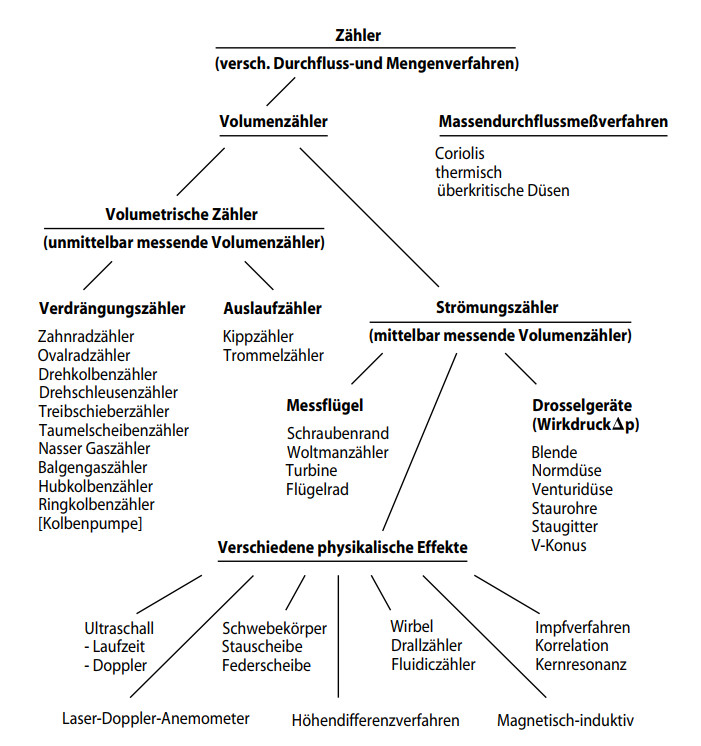
\includegraphics[width=0.75\textwidth]{Bilder/versch_Durchflussmess-Mengenverfahren.jpg}
\caption{Übersicht verschiedener Durchfluss- und Mengenmessverfahren \cite[S. 794]{SensorTechnologien}}
\label{fig:durchfluss_messverfahren} 
\end{figure}




\begin{itemize}
\singlespacing
\item \glqq Kraft auf Körper\grqq{} Durchflussmessung (Volumenstrom, non-digital)
\item Differenzdruckverfahren (Volumenstrom)
\begin{itemize}
\item Lochblende
\item Venturi-Rohr
\end{itemize}
\item Vortexdurchflußmessung (Volumenstrom, für Gase nur in Kombination mit Dichtemessung Massenstrom)
\item thermische Massendurchflussmessung (Massenstrom)
\item Coriolis Durchflussmessung (Massenstrom)
\end{itemize}

\paragraph*{Kraft auf Körper Durchflussmessung} Da ein Versuchsstand im Rahmen dieser Arbeit, zu Beginn des Projekts, einen (\textit{analog}) \textbf{S}chwebe\textbf{k}örper\textbf{d}urchfluss\textbf{m}esser (SKDM; siehe Abbildung \ref{fig:mech_durchflussmesser}) besitzt und eine diversitäre Redundanz, mittels \textit{digitalem} Sensor, erfolgen soll, wird das Wirkprinzip dieses rein analogen Messverfahrens erläutert. Gemäß \cite[S. 827 ff.]{Tränkler2015} wird dieses Messverfahren \glqq Kraft auf Körper genannt\grqq. Ein \textit{Festkörper} wird in einer konischen Rohrleitung angeströmt und wird angehoben oder ausgelenkt, im Falle eines \textbf{Federscheibendurchflussmessers}, bei hinreichend großer Anströmgeschwindigkeit. Eine äquivalente Lösung, ist dass installieren eines  konischen Schwebekörper in eine Blendenöffnung. Sobald sich ein Kräftegleichgewicht einstellt, verharrt der Festkörper in der Position. Die geometrischen Formen der Festkörper können z.B. ein Konus (SKDM) oder eine Scheibe (Federscheibendurchflussmessers) sein \cite[S. 827]{Tränkler2015}. Der abzulesende Volumenstrom ist somit unter anderem eine Funktion des durchströmten Querschnitts $A$. Das physikalische Wirkprinzip ist ein Kräftegleichgewicht. Wenn sich die Gravitationskraft $F_\mathrm{G}$, abzüglich der Auftriebskraft $F_\mathrm{A}$ eines Partikels oder Festkörpers, mit der Widerstandskraft $F_\mathrm{W}$ im Gleich\-gewicht befindet (siehe Gleichung \ref{eq:gleichgewicht}), dann befindet sich die Strömung in einem stationärem Zustand. Für ein frei bewegliches Festkörperpartikel, welches sich im Gravitationsfeld befindet und vertikal von unten angeströmt wird (z.B. SKDM), gilt Gleichung \ref{eq:gleichgewicht} \cite[S. 105 ff.]{Stiess2008}.

\begin{align}
\label{eq:gleichgewicht}
F_\mathrm{G} - F_\mathrm{A} = F_\mathrm{W}
\end{align}

Die Widerstandskraft $F_\mathrm{W}$ eines Festkörpers in einer Strömung lautet:

\begin{align}
\vec{F}_\mathrm{W} = c_\mathrm{w} (\mathrm{Re}_x) \cdot A \cdot \rho_\mathrm{f} \cdot \frac{\vec{v} \cdot \vert v\vert}{2}
\end{align}

Der $c_\mathrm{w}$ Wert gibt den Widerstand eines Partikels in einer Strömung an. Er ist abhängig von der Form sowie Größe eines Partikels (Index $x$) und ist eine Funktion der Reynoldszahl.\\

\paragraph*{Differenzdruckbasierte Sensoren} Differenzdruckbasierte Sensoren sind robust, bieten eine hohe Prozesssicherheit und sind kostengünstig. Sie
eignen sich besonders für große Durchflussmengen. Dieses Verfahren wird auch Wirkdruckverfahren genannt. Die Nutzung einer \textbf{Lochblende} hat den Vorteil, dass ein großer Messbereich, durch Wechsel bzw. Variation der Lochblende, genauer Durchflussöffnung, realisierbar ist. Für den Betrieb eines differenzdruckbasierten Sensors mittels Lochblende ist zu beachten, dass durch die Drosselung  und die dadurch auftretende Dissipation von Energie, hohe Betriebskosten entstehen können.
\textbf{Venturi-Rohre} haben eine bessere Energiebilanz gegenüber Lochblenden. Des Weiteren weisen Venturi-Rohre gegenüber Lochblenden weniger Verschleiß  auf und sind demnach weniger Wartungsintensiv \cite[S. 823 ff.]{Tränkler2015}.


\paragraph*{Sensoren auf Basis der Corioliskraft} Um den Massenstom von Fluiden zu ermitteln, kann sich die, aus dem zweiten newtonschen Axiom hergeleitete, Corioliskraft zu nutze gemacht werden. Die Corioliskraft ist, wie die Zentrifugalkraft, eine Scheinkraft. Die Corioliskraft ($ \vec{F}_c=f(\vec{a}_\mathrm{c}$)\,), zur Bestimmung des Massendurchflusses, ist proportional zur Masse des durchströmten Messrohrs ($\vec{F}_\mathrm{c}=m \cdot \vec{a}_\mathrm{c}$), in der Abbildung \ref{fig:coriolisod} und \ref{fig:coriolisd} ist es das U-Rohr. Das Messrohr wird elektromagnetisch in Schwingung gesetzt. Wird das Messrohr durchströmt, tritt der Coriolis-Effekt auf und das Messrohr oszilliert um die y-Achse (siehe Abbildung \ref{fig:coriolisd}). Für tiefgreifendes Wissen zum Wirkprinzip des Sensors muss auf Fachliteratur verwiesen werden \cite[S. 268 ff.]{SensorTechnologien}.

\begin{figure}[p!] 
\centering
%\hspace{0em}
%\captionsetup{position=top}

     \subfloat[][Schwebekörperdurchflussmesser~(\texttt{links}) \newline Federscheibendurchflussmesser~(\texttt{rechts})\label{fig:mech_durchflussmesser}]{%
       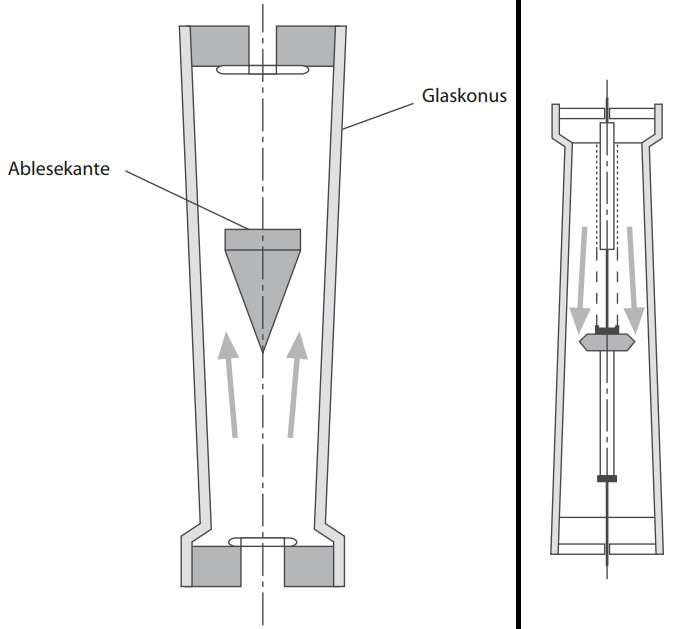
\includegraphics[width=0.40\textwidth]
       {Bilder/mechanische_durchflussmesser.jpg} %{Bilder/LabVIEW_serialport/}
     }%\hspace{-1.5pt}%
     \hfill     
    \subfloat[][Wirkdruckdrosselgeräte Übersicht nach DIN\label{fig:Wirkdruckverfahren}]{%
       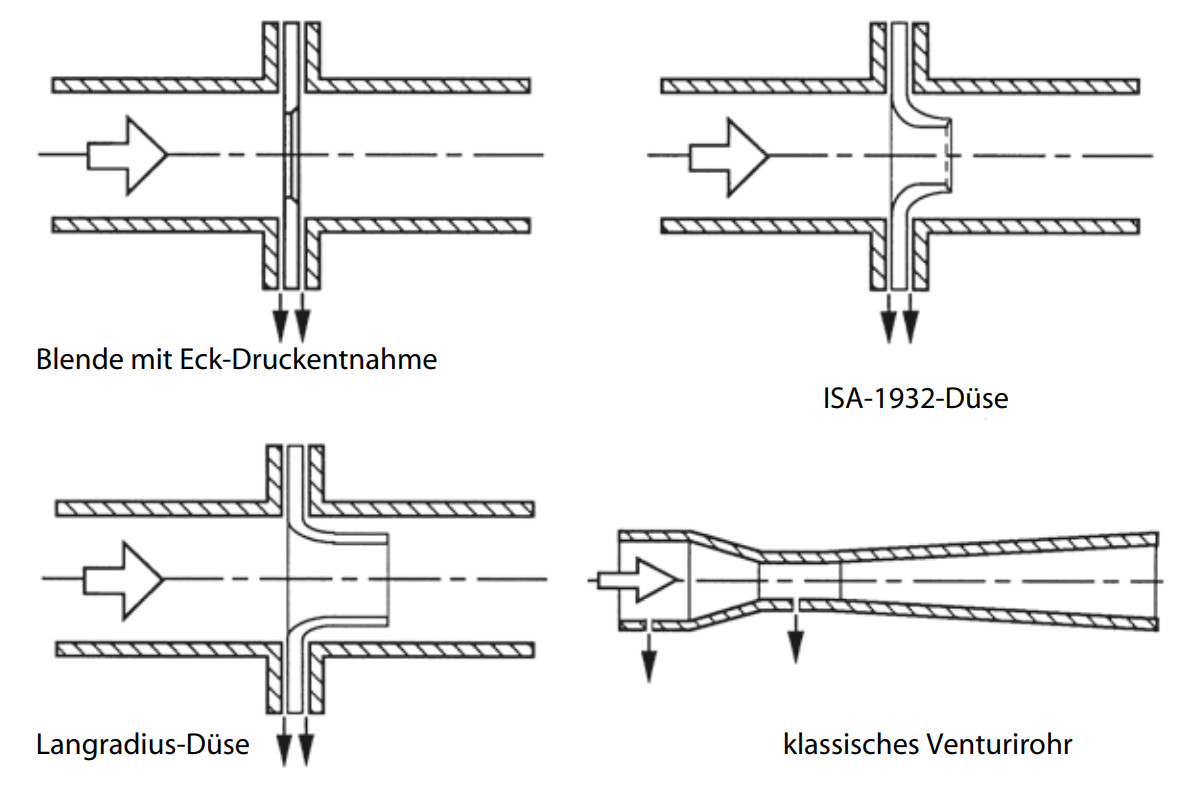
\includegraphics[width=0.45\textwidth]
      {Bilder/Wirkdruckverfahren.jpg}
     }\phantomcaption
%\vspace{-.81em}
\ContinuedFloat

     \subfloat[][angeregter Coriolissensor ohne Durchsatz\label{fig:coriolisod}]{%
       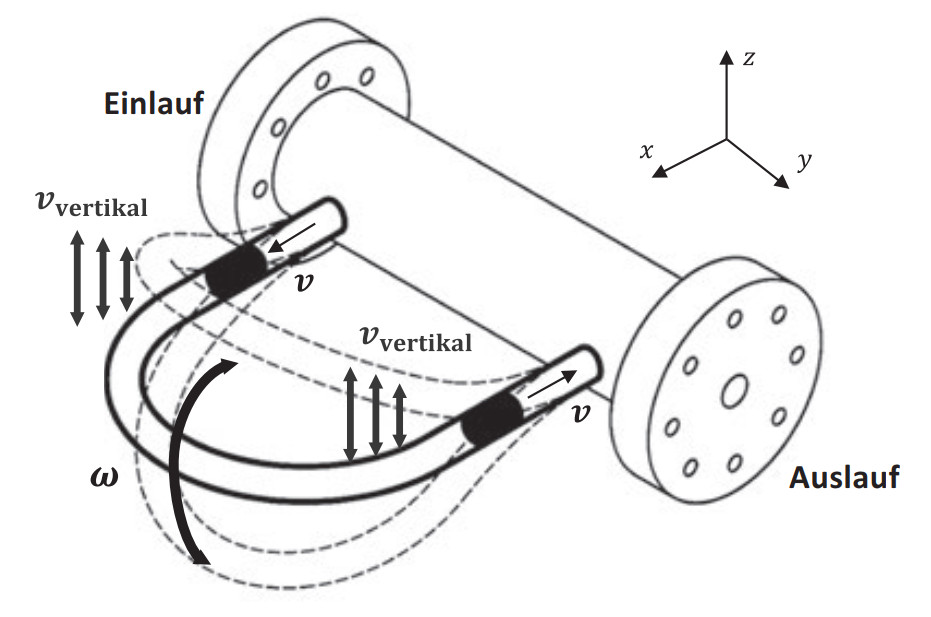
\includegraphics[width=0.45\textwidth]
       {Bilder/coriolis_leer.jpg} %{Bilder/LabVIEW_serialport/}
     }%\hspace{-1.5pt}%
     \hfill     
    \subfloat[][angeregter Coriolissensor mit Durchsatz\label{fig:coriolisd}]{%
       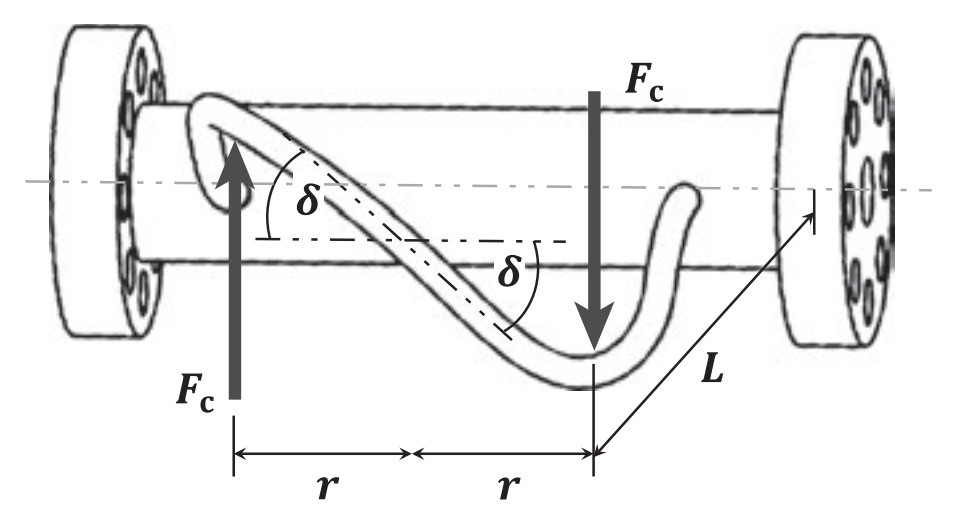
\includegraphics[width=0.45\textwidth]
      {Bilder/coriolis_durchsatz.jpg}
     }\phantomcaption
%\vspace{-.81em}
\ContinuedFloat
\captionsetup{position=bottom}
\subfloat[position=top][Vortexsensor\label{fig:vortexsensor}]{%
       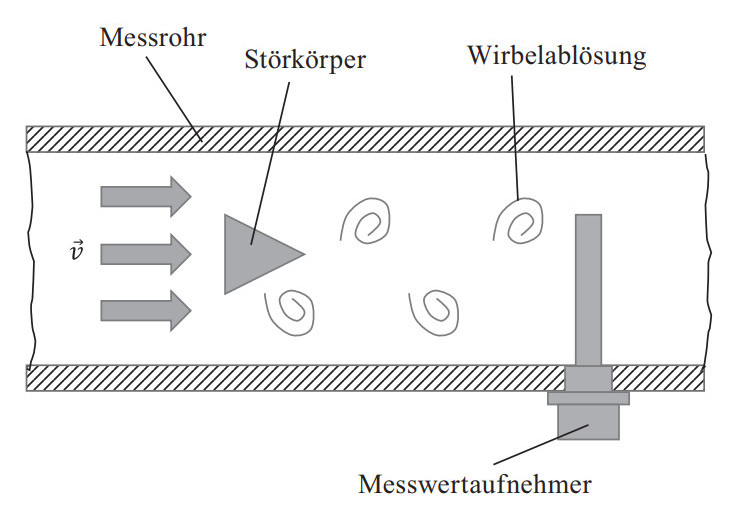
\includegraphics[width=0.45\textwidth]
       {Bilder/vortexsensor.jpg}
     }%\hspace{-1.6pt}%
     \hfill     
    \subfloat[position=top][Drallsensor \label{fig:drallsensor}]{%
       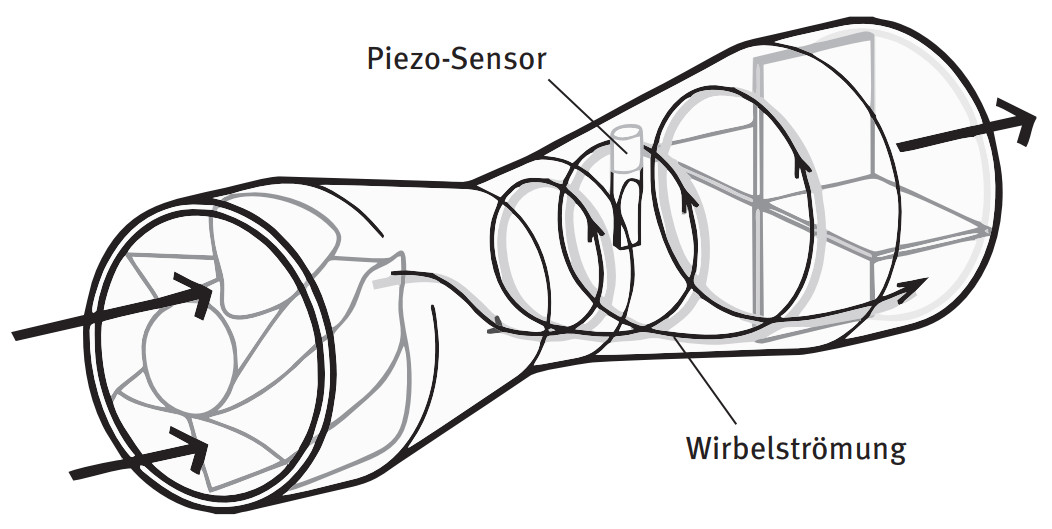
\includegraphics[width=0.45\textwidth]
      {Bilder/drallsensor.jpg} %{Bilder/LabVIEW_serialport/}
     }    
\caption[Übersicht einiger Sensoren, die für die Messung von Gasdurchflüssen geeignet ist]
{Übersicht einiger Sensoren, die für die Messung von Gasdurchflüssen geeignet ist:
(a) Mechanische Durchflusssensoren
(b) Wirkdruckverfahren \cite[S. 826]{Tränkler2015},
(c, d) Coriolisensor \cite[S. 270]{SensorTechnologien}
(e, f) Vortex- sowie Drallsensor}
\label{fig:Sensorübersicht}
   \end{figure} 

\paragraph*{Vortexdurchflusssensoren} Die industrielle Nutzung von Vortexdurchflußsensoren (Wirbelsensoren, siehe Abbildung \ref{fig:vortexsensor}) begann in den 1960er-Jahren.  Das physikalische Grundprinzip ist die Kármánsche Wirbelstraße. Das Wirkprinzip beruht auf der Anregung eines Störkörpers, wie eines Drahtes, in einer Strömung. Die Schwingfrequenz ist proportional zur Anströmgeschwindigkeit und antiproportional zur Dicke des Drahtes. Die Ursache der Schwingung ist die Wirbelablösung hinter einem Strömungswiderstand. Die Geometrie des Störkörpers beeinflusst die Wirbelbildung und somit die Schwingung maßgeblich. Bei der Durchflussbestimmung von Gasen ist eine Sensornahe Bestimmung der Dichte erforderlich, da durch die Kompressibilität von Gasen, Dichtedifferenzen auftreten können, die sich maßgeblich auf die gemessene Durchsatzmenge auswirken. Für Gase ist der Vortexsensor, durch die Kombination mit einer Dichtemessung, somit nur als Massendurchflusssensor geeignet. Eine Weiterentwicklung des Vortexdurchflussensors ist der Drallsensor (siehe Abbildung \ref{fig:drallsensor}). Durch den induzierten Drall kann die Einlaufstrecke signifikant verkürzt werden \cite[S. 294 ff.]{SensorTechnologien}.




\paragraph{Thermischer Massendurchflusssensor}

Die Durchflussmessung von Gasen ist mittels thermischen Massendurchflussmesser möglich. Zur Messung des Massendurchflusses wird die Wärmeleitfähigkeit des zu messenden Fluids genutzt. Der prinzipielle Aufbau so eines Sensors ist in Abbildung \ref{MFC} dargestellt.

\bild{0.45}
{MFC.jpg}
{0em}
{Prinzip eines thermischen Massendurchflussensors}
{Prinzip eines thermischen Massendurchflussensors \cite[S. 656]{Wiegleb2016}}
{MFC}

Auf das Messprinzip dieses Sensors wird genauer eingegangen, da er im Rahmen dieses Projekts und in den folgenden Praxisveranstaltungen verwendet wird. Im Inneren des Durchflussmessers sind zwei Temperatursensoren verbaut. Ein Sensor befindet sich nicht direkt im Strömungskanal (in einem Sackloch) und misst die Veränderung der Umgebungstemperatur $T_\mathrm{U}$, als auch die Wärmeübertragung des Fluids als Referenz. Der zweite Sensor wird beheizt. Die Temperaturdifferenz $\Delta T$ wird konstant gehalten. Je höher die Fließgeschwindigkeit des Mediums, desto mehr Energie muss dem zweiten Sensor zugeführt werden, um die Temperaturdifferenz konstant zu halten.  Der Massenstrom $\dot{m}$ ist dem Wärmestrom $\dot{Q}$ proportional. Es gilt folgender Zusammenhang zwischen Massen- und Wärmestrom:

\begin{align}
\dot{Q}=\dot{m} \cdot c_\mathrm{p} \cdot  \Delta T
\end{align}

Der Massenstrom ist der zugeführten Energie in Form von Strom $I^2$ proportional. Der zweite Sensor hat einen temperaturabhängigen Widerstand $R(T)$. 

\begin{align}
\dot{m}=\dfrac{R(T) \cdot I^2}{c_\mathrm{p} \cdot \Delta T}
\end{align}

Beide Sensoren sind zu einer Wheatstone'schen Messbrücke verschaltet, $\sqrt{\dot{m}}$ ist der Ausgangsspannung $\Delta U_{\mathrm{Br}}$ proportional \cite[S. 656]{Wiegleb2016}.

\vspace{2em} 

\subsubsection{Druckmessung}

In der Industrie ist die Bestimmung von Drücken eine fundamentale Messoperation. Bis in die sechziger Jahren wurde der Druck in der Industrie mittels mechanischen Manometern bestimmt. Diese Technologie wurde daraufhin von den sog. Druckaufnehmern, mittels \textbf{D}ehnungs\textbf{m}ess\textbf{s}treifen (DMS) des Werkstoffs Metall oder Drucksensoren, unter der Verwendung von Halbmetallen, abgelöst.  

\paragraph*{Dehnungsresistive Sensoren}

Drucksensoren mittels DMS sind sog. \textit{dehnungsresistive} Drucksensoren. Dehnungsresistive Sensoren nutzen elektrisch Leitende Werkstoffe bzw. Metalle. Das Messprinzip beruht auf der Änderung des elektrischen Widerstandes $R$, eines elektrisch leitenden Werkstoffs, als Folge einer mechanischen Verformung. Es existieren drei Drucksensortechnologien auf Metallbasis.

\begin{enumerate}[label = \textbullet , itemsep = -0.1em]
\item \textcolor{black!60}{DMS aus Draht} 
\item Metallfolien-DMS
\item Dünnfilm-DMS
\end{enumerate}

In den Jahren von 1938 bis zum Ende der 50er Jahre bestand der DMS aus einem Draht, der mäanderförmig auf einen Dehnkörper aufgebracht wurde. Der Draht wurde von Metallfolien und später Dünnfilm-DMS \textcolor{black!60}{abgelöst} \cite[S. 434]{Tränkler2015}. Zur Erläuterung des physikalischen Wirkprinzips wird als Modell ein zylinderförmiger Körper genutzt. 

%\begin{figure}[h!]
%\centering
%\includegraphics[0.9\textwidth]{Bilder/drahtmodell.jpg}
%\caption{Drahtmodell zur Herleitung des Wirkprinzips}
%\label{fig:drahtmodell} 
%\end{figure}

\subparagraph*{Zylindermodell} Ein zylinderförmiger, elektrisch leitender Werkstoff, charakterisiert durch die Ausgangslänge $l_\mathrm{0}$, Ausgangsquerschnitt $A_\mathrm{0}$ und dem spezifischem elektrischem Widerstand $\rho_{\mathrm{el}}$, hat einen elektrischen Widerstand R gemäß folgender Gleichung \cite[S. 4 ff.]{Wolff2016}:

\begin{align}
\label{eq:zyl_wiederstand}
R=\rho_{\mathrm{el}} \cdot \frac{l_\mathrm{0}}{A_\mathrm{0}}
\end{align}

Von diesem Modell ausgehend wird die relative Widerstandsänderung $\Delta R / R$, durch die Bildung des totalen Differenzials, berechnet. Die Lösung der Differenzialgleichung, gemäß \cite[S. 7 ff.]{Wolff2016} (siehe Anhang Gleichung (\ref{eq:totaldif_dms}), unter der Definition einiger Randbedingungen, führt zur Gleichung (\ref{eq:delta}). 
%
%
%\begin{align}  
%\label{eq:totaldif_dms}
%	dR &=\frac{\partial R}{\partial \rho_{el}} \: d\rho_{el}+\frac{\partial R}{\partial l_0} \: dl_0+\frac{\partial R}{\partial A} \: dA \\[1em]
%		&= \frac{l_0}{A} ~ d\rho_{el} + \frac{\rho_{el}}{A} \: dl_0 - \frac{\rho_{el} \cdot l_0}{A^2} \: dA \\[1em]
%		&= R \cdot ( \frac{d\rho}{\rho} + \frac{dl_0}{l_0} - \frac{dA}{A} )
%\end{align}
%
%
%Ersetzt man das Infinitisimal $d$ durch eine eine größere Schrittweite $\Delta$, unter der Bedingung dass $\Delta \rho \ll \rho,\, \Delta l_0 \ll l_0, \Delta A \ll A$, dann erhält man Gleichung \ref{eq:delta}. 

\begin{align}
\label{eq:delta}
\frac{\Delta R}{R} = \frac{\Delta \rho_{\mathrm{el}}}{\rho_{\mathrm{el}}} + \frac{\Delta l}{l_\mathrm{0}} - \frac{\Delta A}{A_\mathrm{0}}
\end{align}

Die geometrische Verformung wird durch die beiden letzten Terme repräsentiert. Die Längendehnung $\psi_\mathrm{L}$ ersetzt $\Delta l / l_\mathrm{0}$ und der Term $\Delta A/A_\mathrm{0}$ wird durch die \textit{Querkontraktion}, Gleichung (\ref{eq:querkontraktion}), mit der \textit{Querkontraktionszahl} $\nu$ ($-\psi_\mathrm{L} / \psi_\mathrm{Q}$), auch Poisson-Konstante genannt, beschrieben. Die mathematische Umformung des Terms  $\Delta A/A_\mathrm{0}$ , unter Anwendung von Gleichung (\ref{eq:querkontraktion}), führt zur Gleichung (\ref{eq:querkontraktion_A}) .

%\begin{equation}
 \begin{align}
 \psi_\mathrm{Q} &= \frac{\Delta D}{D_\mathrm{0}} = - \nu \cdot \psi_\mathrm{L} \label{eq:querkontraktion} \\[1em] 
\frac{\Delta A}{A_\mathrm{0}} &=2\psi_\mathrm{Q} = -\, 2 \cdot \nu \cdot \psi_\mathrm{L}  \label{eq:querkontraktion_A}
\end{align}
%\end{equation}

Durch Einsetzen der Gleichung (\ref{eq:querkontraktion_A}) und der mechanischen Dehnung $\psi_\mathrm{L}$ in die Gleichung (\ref{eq:delta}) erhält man:

\begin{align}
\label{eq:wiederstand_substi}
\frac{\Delta R}{R} =\frac{\Delta \rho_{\mathrm{el}}}{\rho_{\mathrm{el}}} + (1+2\nu) \cdot \psi_\mathrm{L}
\end{align}

Der Term $\Delta \rho_{\mathrm{el}} / \rho_{\mathrm{el}}$ \, ist der sog. \textit{piezoresistive Anteil} $\bigl($präzisiert in Abschnitt \textbf{Halbleiter Drucksensoren}, Gleichung (\ref{eq:piezoeffekt})$\bigr)$, der bei metallischen Leitern \textcolor{black!70}{vernachlässigbar} ist, jedoch bei Halbleitern einen signifikanten Einfluss hat. Wird nun die sog. \textit{Dehnungsempfindlichkeit}  (\textit{engl. gauge-factor}) $k$ eingeführt, erhält man folgende Gleichung (für DMS auf Metallbasis wird der Term \textcolor{black!70}{$\Delta \rho_{\mathrm{el}} / \rho_{\mathrm{el}}$} als 0 angenommen):

\begin{align}
\label{eq:metall_dms}
\frac{\Delta R}{R} &= \underbrace{ \left(1+2\nu \textcolor{black!60}{~+~\frac{\Delta \rho_{\mathrm{el}}}{\rho_{\mathrm{el}}}} \cdot {\psi_\mathrm{L}}^{-1} \right) }_{\substack{=k}} \cdot \: \psi_\mathrm{L} 
\end{align}

Im allg. ist die Dehnungsempfindlichkeit $k$ nicht konstant, da sie eine Funktion der mechanischen Verformung eines elektrisch leitenden Werkstoffs ist. Für metallische Leiter liegt der Wert von $k$ zwischen 2 und 6 und kann bei vielen DMS als eine Konstante angenommen werden. Bei Halbleiter-DMS kann der $k$ Faktor 50 mal größer sein und weist dadurch, aufgrund der Abhängigkeit von der Dehnung, eine signifikante Nichtlinearität auf. Eine Wheatstone-Brücke wandelt die Widerstandsänderung $\Delta R$ in eine proportionale Spannungsänderung um \cite[S. 434 ff.]{Tränkler2015}. \\

\subparagraph*{Quadermodell} Der Draht als DMS wurde in den 50er Jahren von den Metallfolien-DMS; mit den Dimensionen Länge $L$, Breite $b$, Höhe $h$; ersetzt, dessen elektrischer Widerstand sich wie folgt berechnet: 

\label{sec:quader}

\begin{align}
R &= \rho_{\mathrm{el}}~\frac{L}{b \cdot h}  
\label{eq:r_quader} \\[1em] 
\breve{R} (\psi_\mathrm{L} ) &= \rho_{\mathrm{el}}  (\psi_\mathrm{L})~\frac{L (1+\psi_\mathrm{L})}{b \cdot h(1- \nu \cdot \psi_\mathrm{L})^2}
\label{eq:spez_quader_exakt}
\end{align}

Auf die Herleitung des exakten elektrischen Widerstands $\breve{R}$ der Gleichung  \ref{eq:spez_quader_exakt} wird im Rahmen dieser Arbeit verzichtet. Mechanische Dehnungen $\psi_\mathrm{L}$ in Längsrichtung sind im technisch relevanten Bereich kleiner 0,1 \%. Für diese Dehnungen kann der nichtlineare Term vernachlässigt werden. Für die Linearisierung des spez. elektrischen Widerstands eines Quaders, wird das totale Differenzial des elektrischen Widerstands (Gleichung \ref{eq:r_quader}) gebildet. Die Lösung ist Gleichung \ref{eq:spez_quader_diff} \cite[S. 42 f.]{Nolten2013}. 

\begin{align}
\frac{\Delta R}{R} &= \frac{\Delta \rho_{\mathrm{el}}}{\rho_{\mathrm{el}}} \underbrace{- \frac{\Delta b}{b} - \frac{\Delta h}{h}}_{\substack{=-2 \, \nu \, \psi_\mathrm{L}}} +  \underbrace{\frac{\Delta L}{L}}_{\substack{=\psi_\mathrm{L}}}
\label{eq:spez_quader_diff} \\[1em] 
&=\underbrace{\frac{\Delta \rho_{\mathrm{el}}}{\rho_{\mathrm{el}}} + (1+2\nu)}_{\substack{=k}} \cdot \psi_\mathrm{L} 
\end{align}
% 


Wie zu Beginn dieses Abschnitts erwähnt, existieren neben den DMS aus Metallfolie, ebenfalls Dünnfilm-DMS. Durch die Dünnfilmtechnologie können, gegenüber den Metallfolien-DMS, kleinere Messbereiche erschlossen werden. Der Fertigungsaufwand von Dünnfilm-DMS ist signifikant höher \cite[S.~444~ff.]{Tränkler2015}. Für genauere Information muss an Fachliteratur verwiesen werden.

\paragraph{Halbleiter Drucksensoren} 

Neben den metallischen Drucksensoren, existieren Drucksensoren aus Halbleitern. Es existieren die folgenden zwei Drucksensortechnologien auf Halbleiterbasis:

\begin{enumerate}[label = \textbullet , itemsep = -0.1em]
\item piezoresistive Drucksensoren
\item kapazitive Drucksensoren
\end{enumerate}

Eine Tabelle mit den Kenndaten von \textit{piezoresistiver} und \textit{kapazitiver} Drucksensoren befindet sich im Anhang in der Tabelle \ref{tab:piezo_kapa}.\\

Wie im vorherigen Abschnitt erwähnt, ist die Dehnungsempfindlichkeit $k$ bei Halbleitern nicht als eine Konstante anzunehmen. Der \textit{piezoresistive Anteil} $\Delta \rho_{\mathrm{el}}/\rho_{\mathrm{el}}$ ist eine Funktion der longitudinalen (Index $\mathrm{l}$) und transversalen (Index $t$) mech. Spannungszuständen $\sigma_{\mathrm{l,t}}$ und den \textit{Piezokonstanten} $\pi_{\mathrm{l,t}}$ eines elektrisch leitenden Feststoffs, gemäß Gleichung (\ref{eq:piezoeffekt}):

\begin{align}
\label{eq:piezoeffekt}
\frac{\Delta \rho_{\mathrm{el}}}{\rho_{\mathrm{el}}} = \sigma_{\mathrm{l}} \cdot \pi_\mathrm{l} +\sigma_{\mathrm{t}} \cdot \pi_\mathrm{t}
\end{align}




\newpage 
\subsection{Verfahrenstechnischer Prozess: Durchströmung von Schüttungen}
\label{sec:filterkuchen}
Für die Durchströmung poröser Schichten existieren zwei unterschiedliche Ansätze.

\begin{itemize}
\item Das Modell des hydraulischen Durchmessers.
\item Das Modell der Einzelkornumströmung. 
\end{itemize}

Eine Partikelschicht wird auch Schüttung oder Festbett genannt. Aus dem Modell des hydraulischen Durchmessers wurden diverse empirische Gleichungen abgeleitet, die sich maßgeblich von Ihrem Gültigkeitsbereich unterscheiden. Mit den empirischen Gleichungen werden  strömungsmechanische Effekte nicht mit abgebildet, die in dem Modell der Einzelkornumströmung implementiert sind. Für viele Anwendungen reicht die Approximation, durch Nutzung einer empirischen Gleichung aus. Bei der Auswahl einer empirischen Gleichung sind die Gültigkeitsbereiche und Randbedingungen zu beachten. \\

Gleichungen zur Beschreibung von Schüttungsdurchströmungen geben den Zusammenhang aus folgenden Variablen an \cite[S. 144]{Stiess2008}:

\begin{itemize}
\item eine charakteristische Durchströmungsgeschwindigkeit $w$, bspw. die mittlere Leerrohrgeschwindigkeit ($\bar{v}=\dot{V}/A_\mathrm{a}$)
\item eine Druckdifferenz $\Delta p$
\item Fluideigenschaften, wie die Fluiddichte  $\rho_\mathrm{f}$ und Viskosität  $\eta$
\item und Schichtbeschreibende Geometrien, wie:
	\begin{itemize}
	\item Feinheitsmerkmal $x$ der Partikel, oftmals der Sauterdurchmesser $d_{32}$
	\item die Porösität $\varepsilon$
	\item die Schichthöhe $\Delta L$
	\item der Anströmboden oder die Anströmfläche $A_\mathrm{a}$
	\item ... 
	\end{itemize}
\end{itemize}

Ein Dimensionsanalyter Ansatz zur Eruierung von Durchströmungsgleichungen führt, unter der Anwendung des Buckingham'schen \mbox{$\Pi$-Theorems}, zu den folgenden dimensionslosen Kennzahlen:

\begin{align}
\Pi_1	&\equiv \frac{\Delta p}{\rho \cdot w^2} = \mathrm{Eu} & &\mathrm{(Eulerzahl)} \label{eq:eulerpi}\\[1em]
\Pi_2	&\equiv \frac{w \cdot x \cdot \rho}{\eta} = \mathrm{Re}& &\mathrm{(Reynoldszahl)} \\[1em]
\Pi_3	&\equiv \frac{\Delta L}{x}																& &\mathrm{(Längensimplex)} \\[1em]
\Pi_4	&\equiv \varepsilon = \frac{V_\mathrm{H}}{V} = \frac{1-V_{\mathrm{fs}}}{V} & &\mathrm{(Porösität)} \label{eq:porösität}
\end{align}

Die \textit{Porösität} $\varepsilon$ ist das Verhältnis von Hohlraumvolumen $V_\mathrm{H}$ zu Gesamtvolumen $V$ und kann gemäß Gleichung (\ref{eq:porösität}) berechnet werden. Der Feststoff oder Partikel wird im folgenden mit $\mathrm{fs}$ indiziert  \cite[S. 146]{Stiess2008}. \\

Zur Beschreibung von Partikeln nutzt man Feinheitsmerkmale. Der Sauterdurchmesser $d_{32}$ wird in vielen Gleichungen zur Beschreibung von Partikeln verwendet. Der mittlere Sauterdurchmesser $\bar{d}_{32}$ einer Schüttung kann sich, \textbf{für Partikel die keine hohe Porösität (signifikant hohe Partikeloberfläche) aufweisen}, gemäß Gleichung (\ref{eq:sauter2}) aus einer Partikelgrößenverteilung berechnen lassen. Das Volumen des i-ten Partikelgrößenintervalls ist mit $V_i$ gekennzeichnet \cite[S. 1426 ff.]{vdiwaermeatlas2019}. \vspace{0.8em}

\begin{equation}
\label{eq:sauter2}
\bar{d}_{32}=\Biggl[\sum_{i=1}^N~\Biggl(\frac{V_i}{V} \cdot \frac{1}{d_{32_i}}\Biggr) \Biggr]^{-1}
\end{equation}

\vspace{0.8em} Der \textit{hydraulische Durchmesser} $d_\mathrm{h}$ steht mit dem Sauterdurchmesser $d_{32}$ und der \textit{spezifischen Oberfläche} $S_\mathrm{V}$ im folgendem Zusammenhang \cite[S. 144]{Stiess2008}. \vspace{-0.5em}

\begin{align}
d_\mathrm{h} &= 4 \cdot \frac{\varepsilon}{1-\varepsilon} \cdot \frac{1}{S_\mathrm{V}} \\[1em]
d_\mathrm{h} &= \frac{2}{3} \cdot \frac{\varepsilon}{1-\varepsilon}\cdot d_{32}
\end{align}

Der \textit{hydraulische Durchmesser} $d_\mathrm{h}$, ist der mittlere Porendurchmesser einer Schüttung. Das Modell approximiert die Porösität einer Schüttung durch parallele Kanäle, die nicht miteinander in Wechselwirkung stehen \cite[S. 1426 ff.]{vdiwaermeatlas2019}.\\

\subsubsection{Darcygleichung}
\label{sec:darcygleichung}

Neben der Dimensionslosenkennzahl $\varepsilon$, ist die Einführung der Reynoldszahl Re zielführend. Die Reynoldszahl ist das Verhältnis der Trägheitskraft zur Reibungskraft einer Strömung und ist für die Umströmung von Partikeln eines Feinheitsmerkmals $x$ wie folgt definiert.

\begin{equation}
\label{eq:partikel_re}
\mathrm{Re}_x = \frac{\bar{w} \cdot \bar{x} \cdot \rho_\mathrm{f}}{\eta}
\end{equation}

\vspace{0.5em}Als charakteristische Geschwindigkeit wird die Leerrohrgeschwindigkeit $v$ gewählt.\\



In der Strömungslehre, für die Umströmung von \textbf{Einzelpartikeln}, wird zwischen drei Strömungszuständen unterschieden, die in der Realität fließend ineinander übergehen. Bei der Durchströmung von Schüttungen wird zwischen zwei Strömungszuständen. gemäß Abbildung \ref{fig:schuettungsdurchströmung}; zähe Durchströmung (I) und zäh-\textit{turbulente} Durchströmung (II); nach Stieß unterschieden \cite[S. 146]{Stiess2008}. In der Abbildung \ref{fig:schuettungsdurchströmung} ist die Widerstandsfunktion $f(\mathrm{Re, \varepsilon}$) gegen Re aufgetragen. 

\begin{figure}[h!] %[htbp!] 
\centering
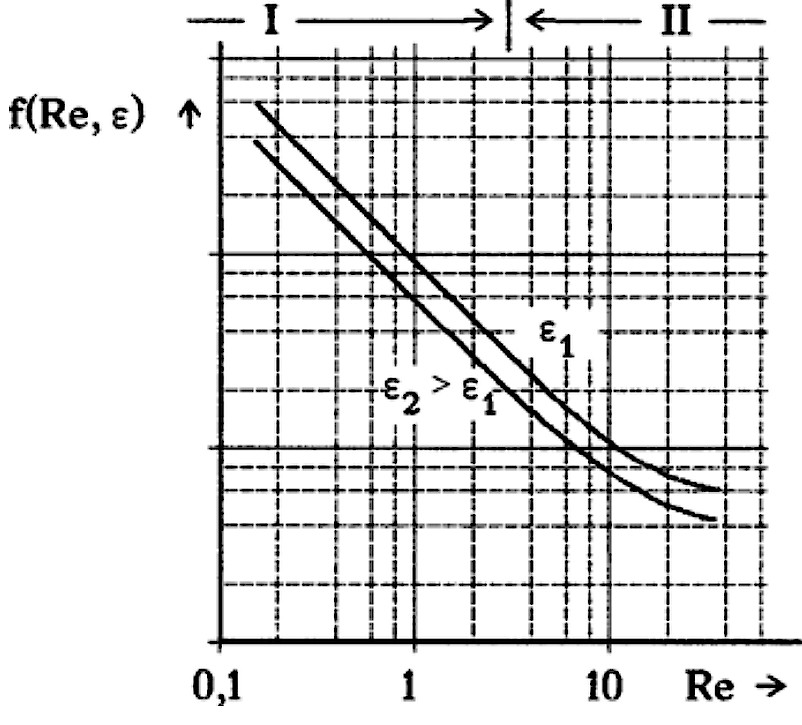
\includegraphics[width=0.4\textwidth]{Bilder/f_von_Re_epsilon.jpg}
\vspace{0em}
 \caption[]{Widerstandsfunktion für die Durchströmung von Schüttgütern, gemäß \cite[S. 146]{Stiess2008}}\label{fig:schuettungsdurchströmung}
\end{figure}

Die Widerstandsfunktion kann gemäß folgender Gleichung berechnet werden: \vspace{-0.3em}

\begin{equation}
\label{eq:widerstandsf_re}
f(\mathrm{Re}_x,\varepsilon)=\frac{\mathrm{Konstante}\,(\varepsilon)}{\mathrm{Re}_x}
\end{equation}

\vspace{0.3em} Die \glqq Konstante\grqq{}, zur Berechnung der Widerstandsfunktion, muss von der Porösität der Schüttung abhängen. Gemäß Abbildung \ref{fig:schuettungsdurchströmung} ist der Grenzwert, zwischen denen die Strömung unterschieden wird, eine Reynoldszahl des Betrags von ca. 3.\\

Die Darcygleichung ist für die Berechnung von strömungsinduzierten Druckverlusten $\Delta p$, zäh durchströmter Schüttungen (I) anwendbar. Unter der Annahme, dass das \mbox{$\Pi$-Theorem} mit den Lösungen $\bigl($Gleichung ($\ref{eq:eulerpi}-\ref{eq:porösität}$)$\bigr)$ nach der Eulerzahl auflösbar ist, das Schüttungen \textit{homogen} sind und \textit{Isotropie} innerhalb der Schüttung vorliegt, gilt Gleichung \cite[S. 145]{Stiess2008}: 

\begin{equation}
\label{eq:euler_pi}
Eu = \frac{\Delta L}{d} \cdot f(\mathrm{Re}_x,\varepsilon)
\end{equation}

\vspace{0.5em} Werden die Gleichungen (\ref{eq:widerstandsf_re}) und (\ref{eq:partikel_re}) in die Eulergleichung (\ref{eq:euler_pi}) engesetzt, erhält man \vspace{0.5em}

\begin{equation}
\label{eq:druck_laenge_darcy}
\frac{\Delta p}{\Delta L} = \frac{\mathrm{Konstante} \, (\varepsilon)}{\bar{x}^2} \cdot 	\eta \cdot \bar{v} .
\end{equation}

\vspace{0.5em} Die Schichteigenschaften werden in der Durchlässigkeit $B$ wie folgt zusammengefasst: \vspace{0.5em}

\begin{equation}
\label{eq:B}
B \equiv \frac{\bar{x}^2}{\mathrm{Konstante}\,(\varepsilon)}
\end{equation}

\vspace{0.3em} Die Durchlässigkeit $B$ muss für jede Schüttung empirisch ermittelt werden und wird in [$m^2$] angegeben. Die Durchlässigkeit charakterisiert die Porenquerschnitte \cite[S. 147]{Stiess2008}. Dadurch vereinfacht sich Gleichung (\ref{eq:druck_laenge_darcy}) zu folgender Gleichung: \vspace{0.5em}

\begin{equation}
\label{eq:druck_laenge_darcy_B}
\frac{\Delta p}{\Delta L} = \frac{\eta \cdot \bar{v} }{B}
\end{equation}


\newpage
\subsubsection{Ableitung der Filtergleichung aus der Darcygleichung}

Um eine Filtergleichung für den Betriebszustand einer konstanten, irreversiblen Druckdifferenz $\Delta p_{\mathrm{irr}}$ zu erhalten, muss die Ableitung gemäß \cite[S.100 ff.]{Stiess2013_verfahrensmechanik_band2} mit folgenden Annahmen erfolgen:


\begin{enumerate}
\item Die Massenkonzentration $c_\mathrm{m}$ bzw. die Volumenkonzentration $c_{\mathrm{vs}}$ der Suspension  bleibt zeitlich und örtlich Konstant,
\item Das gewonnene Filtrat ist Feststofffrei,
\item Der FIlterkuchen weist eine homogene Isotrope Struktur auf,
\item Filterkuchen sowie Filtermittel werden zäh Durchströmt (I).
\end{enumerate}

Das folgende mathematische Modell, zur Ableitung der Filtergleichung, liegt der Abbildung \ref{fig:filtergleichungsmodell} zugrunde.

\begin{figure}[h!] %[htbp!] 
\begin{center}
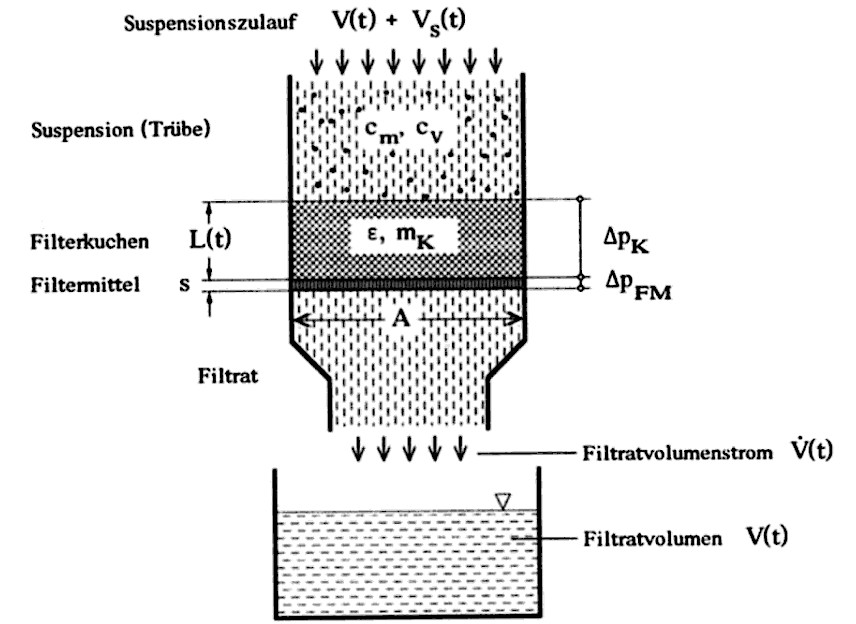
\includegraphics[width=0.7\textwidth]{Bilder/HAW/filterkuchenmodell.jpg}
\end{center}
\vspace{0em}
 \caption[Filterkuchenmodell zur Ableitung der Filtergleichung]{Filterkuchenmodell zur Ableitung der Filtergleichung, gemäß \cite[S.100 ff.]{Stiess2013_verfahrensmechanik_band2}}\label{fig:filtergleichungsmodell}
\end{figure}


Der gesamte irreversible (irr.) Druckverlust $\Delta p_{\mathrm{irr}}$ ist eine Summe aus filterkucheninduziertem $\Delta p_{\mathrm{K}}$ und filtermittelinduziertem  $\Delta p_{\mathrm{FM}}$ Druckverlust.

\begin{equation}
\label{eq:irr_druckverlust}
\Delta p_{\mathrm{irr}} = \Delta p_{\mathrm{K}} + \Delta p_{\mathrm{FM}}
\end{equation}

Der Druckverlust des Filtermittels, mit der Filtermitteldicke $s$ und der Filtermitteldurchlässigkeit $B_{\mathrm{FM}}$, kann gemäß Gleichung (\ref{eq:druck_laenge_darcy_B}) wie folgt berechnet werden:

\begin{equation}
\label{eq:filtermitteldpdt}
\Delta p_{\mathrm{FM}} = \frac{\eta  \cdot s}{B_{\mathrm{FM}}}  \cdot  \frac{\dot{V}}{A}
\end{equation}

\vspace{0.4em} Der Volumenstrom ist im Verlauf der Filtration zeitlich nicht konstant, daher ist das Volumen $V$ über die Zeit zu differenzieren: \vspace{-0.1em}

\begin{equation}
\label{eq:filtermitteldpdt}
\Delta p_{\mathrm{FM}}(t) = \frac{\eta   \cdot s}{B_{\mathrm{FM}} \cdot A}  \cdot  \frac{ \mathrm{d}\, V}{\mathrm{d}\, t}
\end{equation}

\vspace{0.6em} Analog ist zur Berechnung des Druckverlustes durch den Filterkuchen, mit der zeitlich anwachsende Filterkuchendicke  $L(t)$ und dessen Durchlässigkeitskonstante $B_{\mathrm{FM}}$ (unter der Annahme von \textit{Isotropie} und \textit{Homogenität}), folgender Ansatz zu wählen: \vspace{-0.1em}

\begin{equation}
\label{eq:filterkuchendpdt}
\Delta p_{K}(t) = \frac{\eta   \cdot L(t)}{B_{\mathrm{K}} \cdot A}  \cdot  \frac{ \mathrm{d}\, V}{\mathrm{d}\, t}
\end{equation}

\vspace{0.4em} Summiert man Gleichung (\ref{eq:filtermitteldpdt}) und Gleichung (\ref{eq:filterkuchendpdt}) erhält man Gleichung (\ref{eq:irr_druckverlust_dpdt}).

\begin{equation}
\label{eq:irr_druckverlust_dpdt}
\Delta p_{\mathrm{irr}}(t) =  \frac{\eta}{A} \cdot \Biggl[ \frac{L(t)}{B_\mathrm{K}}+\frac{s}{B_{\mathrm{FM}}} \Biggr] \cdot  \frac{ \mathrm{d}\, V}{\mathrm{d}\, t}
\end{equation}

\vspace{0.6em} Durch die Einführung des Filtermittelwiderstandes $\beta=s/B_{\mathrm{FM}}$ und des spezifischen Filterkuchenwiderstands $\alpha_\mathrm{V}= 1/B_\mathrm{K}$ vereinfacht sich Gleichung (\ref{eq:irr_druckverlust_dpdt}) zu: \vspace{0.1em}

\begin{equation}
\label{eq:irr_alpha_beta_dpdt}
\Delta p_{\mathrm{irr}}(t) =  \frac{\eta}{A} \cdot \Bigl[ \alpha_\mathrm{V} \cdot L(t) + \beta \Bigr] \cdot  \frac{ \mathrm{d}\, V}{\mathrm{d}\, t}
\end{equation}

\vspace{0.6em} Unter der Voraussetzung (1) sowie (3), dass das Kuchenvolumen $V_\mathrm{K}$ und das Filtratvolumen $V$ in einer direkt proportionalen Beziehung zueinander stehen ($V_\mathrm{K} \sim V$), kann die Proportionalitätskonstante $\kappa$ eingeführt werden.
\vspace{0.1em}

\begin{equation}
\label{eq:kappa}
L(t)=\frac{V_\mathrm{K}(t)}{A}=\kappa \cdot \frac{V(t)}{A}
\end{equation}

\vspace{0.4em} Ein weiterer Vorteil der Einführung der Proportionalitätskonstante $\kappa$, ist die Substitution der schwierig zu messenden Filterkuchendicke $L(t)$, durch das Filtratvolumen $V(t)$, die sich präzise bestimmen lässt. Setzt man Gleichung (\ref{eq:kappa}) in Gleichung (\ref{eq:irr_alpha_beta_dpdt}) ein, dann erhält man eine leicht auswertbare Gleichung folgender Form:

\begin{equation}
\label{eq:irr_alpha_beta_kappa_dpdt}
\Delta p_{\mathrm{irr}}(t) =  \frac{\eta}{A} \cdot \Bigl[ \frac{\alpha_V \cdot \kappa}{A} \cdot V(t) + \beta \Bigr] \cdot  \frac{ \mathrm{d}\, V}{\mathrm{d}\, t}
\end{equation}



\vspace{2em} 

\subsubsection{Ableitung der Filtergleichung für die Betriebsweise mit einer konstanten Druckdifferenz}

Filtrationen kann man durch unterschiedliche Betriebsweisen realisieren. In der folgenden Auflistung sind die möglichen Varianten aufgelistet:

\begin{enumerate}[label=\Roman*]
\item \quad Isobar -- $\Delta p = \mathrm{konstant}$,
\item \quad Isochor -- $\Delta V = \mathrm{konstant}$,
\item \quad Polytrop --  $\Delta p$ und $\Delta V$ variabel.
\end{enumerate}

Für die isobare Filtration, mit einer konstanten Druckdifferenz $\Delta p_{\mathrm{konst,irr}}$ gilt der nun folgende Ansatz.

\vspace{0.4em} Durch Trennung der Variablen der Gleichung (\ref{eq:irr_alpha_beta_kappa_dpdt}), erhält man Gleichung (\ref{eq:irr_alpha_beta_kappa_trennung_dpdt}) wodurch man durch Integration Gleichung (\ref{eq:irr_alpha_beta_kappa_integration_dpdt}) erhält.

\begin{align}
\mathrm{d}\,t &=  \frac{1}{\Delta p_{\mathrm{konst,irr}}} \cdot \Bigl[ \frac{\eta \cdot \alpha_\mathrm{V} \cdot \kappa}{A^2} \cdot V(t) + \frac{\beta \cdot \eta}{A} \Bigr] \cdot \mathrm{d}\, V \label{eq:irr_alpha_beta_kappa_trennung_dpdt}\\[1.2em]
t &= \frac{\eta \cdot\alpha_\mathrm{V} \cdot \kappa}{A^2 \cdot 2 \cdot \Delta p_{\mathrm{konst,irr}}} \cdot V^2(t) + \frac{\eta \cdot \beta}{A \cdot \Delta p_{\mathrm{konst,irr}}} \cdot V(t) \label{eq:irr_alpha_beta_kappa_integration_dpdt}
\end{align}

\vspace{0.4em}Löst man Gleichung \ref{eq:irr_alpha_beta_kappa_integration_dpdt} nach $V(t)$ auf, erhält man Gleichung (\ref{eq:filtergleichung_V}), wodurch die zeitlich zunehmende Filtratmenge berechnet wird. Die grafische Darstellung einer Filterkurve ist der Abbildung \ref{fig:filterkurve} zu entnehmen.

\begin{equation}
\label{eq:filtergleichung_V}
V(t)= \sqrt{
\Bigl( \frac{\beta \cdot A}{\alpha_V \cdot \kappa} \Bigr)^2
+ \frac{2 \cdot A^2 \cdot \Delta p_{\mathrm{konst,irr}}}{\eta \cdot \alpha_\mathrm{V} \cdot \kappa} \cdot t
} -\frac{\beta \cdot A}{\alpha_\mathrm{V} \cdot \kappa}
\end{equation}


\begin{figure}[h!] %[htbp!] 
\centering
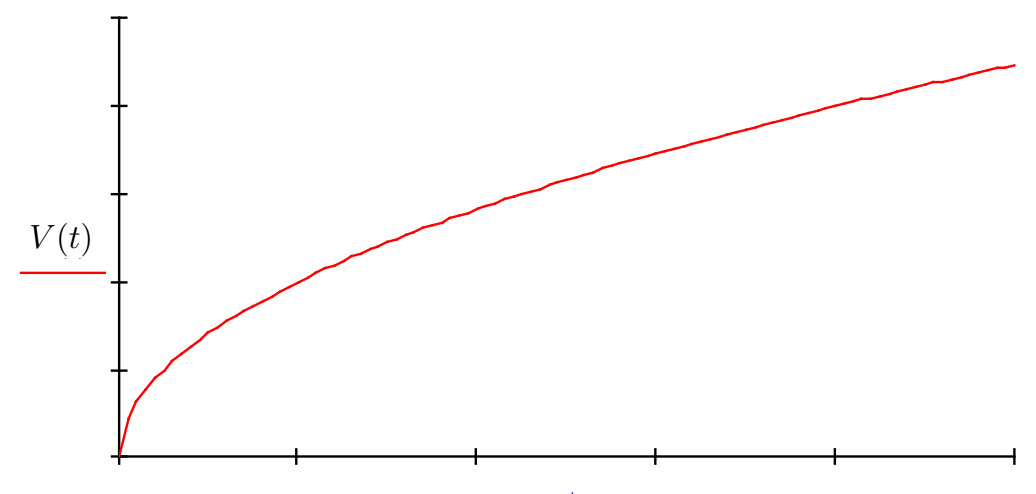
\includegraphics[width=0.7\textwidth]{Bilder/Filterkurve.jpg}
\vspace{0em}
 \caption[]{Filterkurve bei isobarer Betriebsweise \cite[S. 8]{Kuchenfiltration_Geweke2020}}\label{fig:filterkurve}
\end{figure}


Eine weitere Lösung ist die Linearisierung der Gleichung \ref{eq:irr_alpha_beta_kappa_integration_dpdt}, durch Division durch das Volumen als Funktion der Zeit $V(t)$. Die grafische Darstellung der Gleichung (\ref{eq:irr_alpha_beta_kappa_integration_linearisiert_dpdt}) ist der Abbildung \ref{fig:filtergerade_isobarebetriebsweise} zu entnehmen.

\begin{equation}
\label{eq:irr_alpha_beta_kappa_integration_linearisiert_dpdt}
\frac{t}{V(t)} = \underbrace{\frac{\eta \cdot\alpha_\mathrm{V} \cdot \kappa}{A^2 \cdot 2 \cdot \Delta p_{\mathrm{konst,irr}}}
\cdot V(t)}_{\substack{a_1}}  +  \underbrace{\frac{\eta \cdot \beta}{A \cdot \Delta p_{\mathrm{konst,irr}}}}_{\substack{a_0}}
\end{equation}

\begin{figure}[h!] %[htbp!] 
\centering
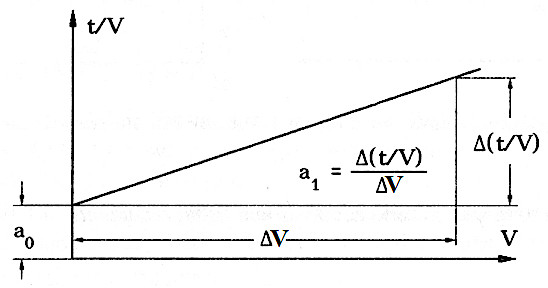
\includegraphics[width=0.7\textwidth]{Bilder/filtergerade.jpg}
\vspace{0em}
 \caption[Filtergerade für die isobare Betriebsweise]{Filtergerade für die isobare Betriebsweise \cite[S.102 ff.]{Stiess2013_verfahrensmechanik_band2}}\label{fig:filtergerade_isobarebetriebsweise}
\end{figure}

%\vspace{0.2em} 

\newpage
Die Ableitungen der Darcy-Gleichung für die isochore (II) oder polytrope (III) Betriebsweise werden im Rahmen dieser Arbeit nicht erläutert.




\paragraph*{Anmerkung}

Neben der Darcy-Gleichung existieren noch weitere empirische Gleichungen, zur Beschreibung von Schüttungen. Die, neben der Darcy-Gleichung, häufig genutzten empirischen Gleichungen werden nachfolgend aufgelistet \cite[S. 148 ff.]{Stiess2008}\cite[S. 1426 f.]{vdiwaermeatlas2019}:

\begin{itemize}
	\item zäh durchströmte Schüttung
	\begin{itemize}
		\item Carman-Kozeny-Gleichung (höherer Detailgrad)
	\end{itemize}
	\item zäh \textit{turbulent} durchströmte Schüttung 
	\begin{itemize}
		\item Ergun-Gleichung
		\item Brauer-Gleichung
	\end{itemize}
\end{itemize}

Das Model der Einzelpartikelumströmung nach \textit{Molerus} kann bspw. dem VDI-Wärmeatlas entnommen werden \cite[S. 1427 ff.]{vdiwaermeatlas2019}.



\newpage
\subsection{Verfahrenstechnischer Prozess: Gas-Feststoff Wirbelschicht}

Das Wirbelschichtverfahren ist eine verfahrenstechnische Grundoperation (\textit{engl. Unit Operation}). Dieses Verfahren wird im Sprachgebrauch der Wirbelschichttechnik auch Fluidisierung (\textit{engl. fluidization}) genannt. Die Fluidisierung wird für verschiedene Zwecke eingesetzt, wie z.B. zum Fördern, Mischen, Agglomerieren \cite{Ding2010}, Trocknen, Rösten, aber auch in der Reaktortechnik, wie zum Verbrennen von Schüttgütern \cite{Reuter2011}. Das Partikelbett (\textit{engl. fixed-bed}) liegt in einem Wirbelschichtapparat auf Anströmböden $A_\mathrm{a}$. Im Labormaßstab entspricht das einem Filtergewebe.

\subsubsection{Festbett-/Wirbelschichtparameter}

Ein Schüttgutpartikelbett, welches keine Anströmung durch ein Fluid erfährt oder keinen fluidähnliches Verhalten hat, wird als Festbett (\textit{engl. fixed-bed}) bezeichnet. Es kennzeichnet sich durch folgende Parameter aus \cite[S. 1561 ff.]{vdiwaermeatlas2019}:

\begin{itemize}
\item das Schüttguttvolumen $V_{\mathrm{fb}}$ 
\item der Masse $m_{\mathrm{fs}}$ 
\item die Dichte der Partikel $\rho_{\mathrm{fs}}$  
\item der Festbettporösität $\varepsilon_{\mathrm{fb}}$, der Partikelgrößenverteilung; die dem Feinheitsmerkmal der Partikel, dem sog. Sauterdurchmesser $d_{32}$ ($d_{32}=6/S_\mathrm{V}$) inhärent ist
\item und der apparatabhängigen Anströmfläche $A_\mathrm{a}$ 
\item Die mittlere Leerrohrgeschwindigkeit $\bar{v}$ 
\end{itemize}

In der Wirbelschichttechnik verwendet man die \textbf{Leerrohrgeschwindigkeit}. Die Leerrohrgeschwindigkeit $\bar{v}$ ist auf die leere Wirbelschichtquerschnittsfläche $A_\mathrm{a}$ bezogene Fluidgeschwindigkeit. 

Des Weiteren werden für die vollständige Berechnung der Wirbelschicht weitere dimensionslose Kennzahlen benötigt, auf die im Rahmen dieser Arbeit nicht weiter eingegangen wird. Nähere Informationen können bspw. dem VDI-Wärmeatlas entnommen werden \cite[S. 1561 ff.]{vdiwaermeatlas2019}.

\subsubsection{Klassifizierung von Schüttgütern nach Geldart}

Nicht alle Schüttgüter sind für Wirbelschichten gleichermaßen geeignet. Geldart hat eine Klassifizierung durchgeführt (siehe Abbildung \ref{fig:geldart}). Im sog. Geldart-Diagramm ist auf der Ordinate die Dichtedifferenz zwischen Fluid und Partikel dargestellt. Auf der Abzisse ist der mittlere Partikeldurchmesser $\bar{d}_{32}$ (gemäß Grafik $d_\mathrm{p}$) aufgetragen. In der Abbildungen sind vier Cluster (C, A, B, D), zwei breite und ein schmaler Übergangsbereich zu erkennen. Das Verhalten der Schüttgüttypen in einer Wirbelschicht unterscheidet sich z.T. signifikant \cite[S. 1566]{vdiwaermeatlas2019}.

\paragraph{Gruppe C} Schüttgüter die nach Klasse C klassifiziert werden, haben kleine mittlere Partikeldurchmesser und weisen größere Haftkräfte auf, als die durch die Strömung induzierte Kraft. Es bilden sich Kanäle aus. Eine Ausbildung einer Wirbelschicht ist nur durch apparative Hilfsmittel oder der Zusatz durch Fließmittel möglich \cite[S. 1566]{vdiwaermeatlas2019}.

\paragraph{Gruppe A} Oberhalb der Lockerungsgeschwindigkeit bildet sich eine homogene WIrbelschicht aus. Wird die Leerrohrgeschwindigkeit weiter erhöht Bilden sich Blasen aus, die sich beim emporsteigen zusammenschließen (Koaleszenz). Die Blasenaufstiegsgeschwindigkeit ist höher als die des Zwischenraumgas und die Blasengröße ist ab erreichen einer bestimmten Betthöhe begrenzt. Wird die Anströmung unterbrochen, kollabiert das Partikelbett langsam \cite[S. 1566]{vdiwaermeatlas2019}. 

\paragraph{Gruppe B}
Unmittelbar nach Überschreiten der Lockerungsgeschwindigkeit bilden sich Blasen aus.  Die Blasenaufstiegsgeschwindigkeit ist höher als die des Zwischenraumgas. Die Blasengröße ist nicht begrenzt. Die Bettausdehnung ist geringer als die der Schüttgüter der Gruppe A. Wird die Anströmung unterbrochen kollabiert das Bett schlagartig \cite[S. 1566]{vdiwaermeatlas2019}. 

\paragraph{Gruppe D}
Die Partikel dieser Gruppe sind groß und weisen eine große Dichte auf. Die Blasen haben eine geringere Aufstiegsgeschwindigkeiten als die des Zwischenraumgases. Nutzt man keinen breiten Anströmboden sondern nur eine Zentrale Bohrung, dann bildet sich bei hinreichend großer Anströmgeschwindigkeit eine Strahlschicht aus \cite[S. 1566]{vdiwaermeatlas2019}.  

\begin{figure}[h!] %[htbp!] 
\centering
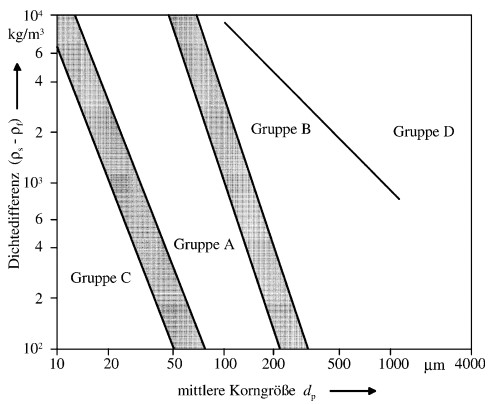
\includegraphics[width=0.6\textwidth]{Bilder/Geldart.jpg}
\vspace{0em}
 \caption[Klassifizierung von Schüttgütern nach Geldart]
 {Klassifizierung von Schüttgütern nach Geldart \cite[S. 1566 ff.]{vdiwaermeatlas2019}}\label{fig:geldart}
\end{figure}


 \pagebreak

 
\subsubsection{Wirbelschichtzustände eines für die Fluidisierung optimalen Schüttguts}

Um die Funktionsweise der Wirbelschicht zu verstehen, werden vier Zustände der Wirbelschicht; anhand eines für die sog. \textit{Fluidisierung} optimalen Schüttguts (Klassifizierung nach Geldart A), gemäß der Abbildung  \ref{fig:wirbelschichtzustände}; beschrieben. In der Abbildung \ref{fig:wirbelschichtzustände} sind Wirbelschichtzustände als Funktion der Anströmgeschwindigkeit schematisch dargestellt \cite[S. 1561 f.]{vdiwaermeatlas2019}.\\

\textbf{Abbildung \ref{fig:wirbelschichtzustände}\texttt{a}} zeigt ein Schüttgutfestbett, welches mit einem $\dot{V}$ Volumenstrom beaufschlagt wird, welcher kleiner ist als der minimale Fluidisiervolumenstrom $\dot{V}_{\mathrm{mf}}$. Die Mehrheit der Partikel befindet sich in Kontakt.\\

Sobald die Anströmgeschwindigkeit der minimalen Fluidisiergeschwindigkeit entspricht, ist der sog. Lockerungspunkt erreicht (\textbf{Abbildung \ref{fig:wirbelschichtzustände}\texttt{b}}). Das Schüttgut nimmt fluidähnliches Verhalten an. Das gesamte, nun Fluidbettbett ist in einer homogenen Bewegung. Es liegt der Zustand der Minimalfluidisation vor.\\


\begin{figure}[t!] %[htbp!] 
\centering
\includegraphics[width=0.85\textwidth]{Bilder/wirbelschichtzustände.jpg}
\vspace{0em}
 \caption[Wirbelschichtzustände als Funktion der Anströmgeschwindigkeit]
 {Wirbelschichtzustände als Funktion der Anströmgeschwindigkeit \cite[S. 1562]{vdiwaermeatlas2019} }\label{fig:wirbelschichtzustände}
\end{figure}



Wird die Strömungsgeschwindigkeit weiter erhöht tritt eine Blasenbildung auf. Welche Form der Blasenbildung entsteht ist unter anderem abhängig von der Geometrie des Apparates (vgl. \textbf{Abbildungen \ref{fig:wirbelschichtzustände}\texttt{c}} und \textbf{\ref{fig:wirbelschichtzustände}\texttt{d}}). Beim Aufsteigen der vereinzelten Gasblasen verschmelzen diese. Dieser Vorgang wird Koaleszenz genannt.\\

Ist die Anströmgeschwindigkeit viel größer als die minimale Fluidisiergeschwindigkeit und erreicht bzw. übersteigt die Sinkgeschwindigkeit der Partikel (Einzelkornsinkgeschwindigkeit), dann bricht die Blasenbildung auf und der Feststoff wird ausgetragen (siehe \textbf{Abbildung \ref{fig:wirbelschichtzustände}\texttt{e}}). Wie in der \textbf{Abbildung} \ref{fig:wirbelschichtzustände}\texttt{e} zu erkennen, bilden sich Feststoffsträhnen, dadurch ist die Aufrechterhaltung der Wirbelschicht möglich. Wenn das Ziel der Wirbelschicht nicht der Partikelförderung entspricht, dann ist eine Rückführung der Partikel, bspw. durch einen nachgeschalteten Zyklon, gemäß \textbf{Abbildung} \ref{fig:wirbelschichtzustände}\texttt{e} zu realisieren.\\

\paragraph{Anmerkung}
Schüttgüter der Geldartklassifizierung C und D benötigen andere apparative Lösungen. Es wird auf Fachliteratur wie bspw. den VDI-Wärmeatlas hingewiesen.\\


\subsubsection{Druckverlust beim Betrieb einer Wirbelschicht}

Die Wirbelschicht wird dadurch ausgezeichnet, dass sich das Partikelbett in einem definierten Volumenstromintervall wie ein Fluid verhält. Das Partikelbett hat in dem Intervall zwischen der \textbf{Lockerungsgeschwindigkeit} $\bar{v}_{\mathrm{mf}}$ und der Partikelaustragsgeschwindigkeit fluidähnliche Eigenschaften. Die Partikelaustragsgeschwindigkeit kann mit der \textbf{Einzelkornsinkgeschwindigkeit} $\bar{w}_{\mathrm{fs}}$ abgeschätzt werden. Das Leerrohrgeschwindigkeitsintervall der Fluidisierung ist somit  $[\bar{v}_{\mathrm{mf}};\bar{v}_{\mathrm{fs}}]$ \cite[S. 1562 ff.]{vdiwaermeatlas2019}. \\

\begin{figure}[b!] %[htbp!] 
\centering
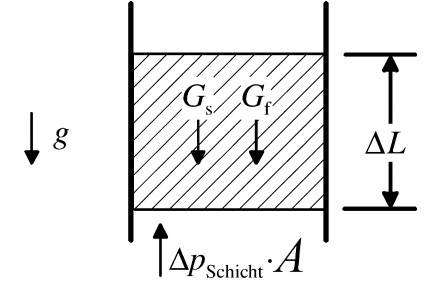
\includegraphics[width=0.5\textwidth]{Bilder/wirbelschicht_kraefte.jpg}
\vspace{0em}
 \caption[]{Wirbelschichtkräfftegleichgewicht an einem Wirbelschichtelement der Länge $\Delta L$ und Anströmfläche $A$, angelehnt an \cite[S. 1562]{vdiwaermeatlas2019}}\label{fig:wirbelschicht_kraefte}
\end{figure}

Der Wirbelschicht liegt ein Kräftegleichgewicht zugrunde. Im stationären Zustand befinden sich die Partikel in der Schwebe. In der Abbildung \ref{fig:wirbelschicht_kraefte} ist das Kräftegleichgewicht eines Wirbelschichtelements skizziert. Das Kräftegleichgewicht eines Wirbelschichtelements der Länge $\Delta L$ und der Anströmfläche $A_\mathrm{a}$ lässt sich wie folgt berechnen.

\begin{equation}
\label{eq:kraefte_ggw_ws}
\Delta P_{\mathrm{Schicht}} \cdot A_\mathrm{a} = G_{\mathrm{fs}} + G_{\mathrm{f}}
\end{equation}

Das Feststoffgewicht $G_{\mathrm{fs}}$ ergibt sich für eine Schicht mit der Feststoffdichte $\rho_{\mathrm{fs}}$ durch

 \begin{equation}
 \label{eq:feststoffgewicht}
G_{\mathrm{fs}}=\rho_{\mathrm{fs}}~(1-\varepsilon)~g~A_{\mathrm{a}}~\Delta L
 \end{equation}

und das Gewicht des Fluids, mit der Fluiddichte $\rho_\mathrm{f}$ durch 

 \begin{equation}
  \label{eq:fluidgewicht}
G_{\mathrm{f}}=\rho_{\mathrm{f}}~\varepsilon~g~A_{\mathrm{a}}~\Delta L.
 \end{equation}
 
Der Druckabfall einer Schicht berechnet sich mit den Gleichungen \ref{eq:feststoffgewicht} und  \ref{eq:fluidgewicht} aus Gleichung \ref{eq:kraefte_ggw_ws} wie folgt:
 
\begin{equation}
\label{eq:druckabfall_schicht}
\Delta P_{\mathrm{Schicht}} = \underbrace{ (\rho_{\mathrm{fs}}-\rho_\mathrm{f})(1-\varepsilon)~g~\Delta L}_{\substack{=\Delta p_{\mathrm{irr}}}} +\underbrace{\rho_\mathrm{f}~g~\Delta L}_{\substack{=\Delta p_{\mathrm{reversibel}}}}
\end{equation}

\vspace{0.8em} Der erste Term repräsentiert den irreversiblen Anteil des Druckabfalls. Um die Partikel in der Schwebe zu halten wird Energie benötigt, die sich anhand des ersten Terms berechnen lässt. Der irreversible Anteil des Druckabfalls setzt sich aus der Gewichtskraft pro Fläche (Gleichung \ref{eq:feststoffgewichtskraft}), abzüglich der volumenstrominduzierten Auftriebskraft pro Fläche  (Gleichung \ref{eq:partikelauftriebskraft}) zusammen \cite[S. 1562 ff.]{vdiwaermeatlas2019}.

 \begin{align}
p_{\mathrm{fs}} &= \rho_{\mathrm{fs}}~(1-\varepsilon)~g~\Delta L \label{eq:feststoffgewichtskraft} \\
p_{\mathrm{f}} &= -\rho_{\mathrm{f}}~(1-\varepsilon)~g~\Delta L \label{eq:partikelauftriebskraft}
 \end{align}

Der zweite Term der Gleichung (\ref{eq:druckabfall_schicht}) repräsentiert die potentielle Energie des geförderten Fluids, der Höhe $\Delta L$. Diese \mbox{Energie} kann im Falle einer Flüssig-Feststoffwirbelschicht, bspw. durch die Nutzung einer Turbine, zurückgewonnen werden \cite[S. 1562 ff.]{vdiwaermeatlas2019}. \\

Die Leerrohrgeschwindigkeit der Minimalfluidisation $v_{\mathrm{mf}}$, auch Lockerungsgeschwindigkeit genannt, kann empirisch ermittelt werden. Wird der dimensionslose Druck gegen die Leerrohrgeschwindigkeit aufgetragen, ist die Lockerungsgeschwindigkeit mit dem erreichen des dimensionslosen Drucks mit dem Betrag von 1 erreicht (siehe Abbildung \ref{fig:lockerungsgeschwindigkeit}). Ab dem Überschreiten der Leerrohrgeschwindigkeit ist der Druckverlust, relativ zur Umgebung $\Delta p$ ebenfalls konstant, dazu wird eine doppelt logarithmische Auftragung empfohlen. Simultan zum Anstieg der Leerrohrgeschwindigkeit, ab der Lockerungsgeschwindigkeit $v_{\mathrm{mf}}$, ist eine Expansion der Wirbelschicht messbar. Die Druckkonstanz ab dem Lockerungspunkt ist damit zu erklären, dass die erhöhte Energiezufur für die Expansion der Wirbelschicht genutzt wird. Ab einer bestimmten Expansion schließen sich Hohlräume zusammen und es kommt zur Blassenbildung (siehe Abbildung \ref{fig:wirbelschichtzustände}). Dieser Effekt liegt der Koalesenz zugrunde.

\begin{figure}[t!] %[htbp!] 
\centering
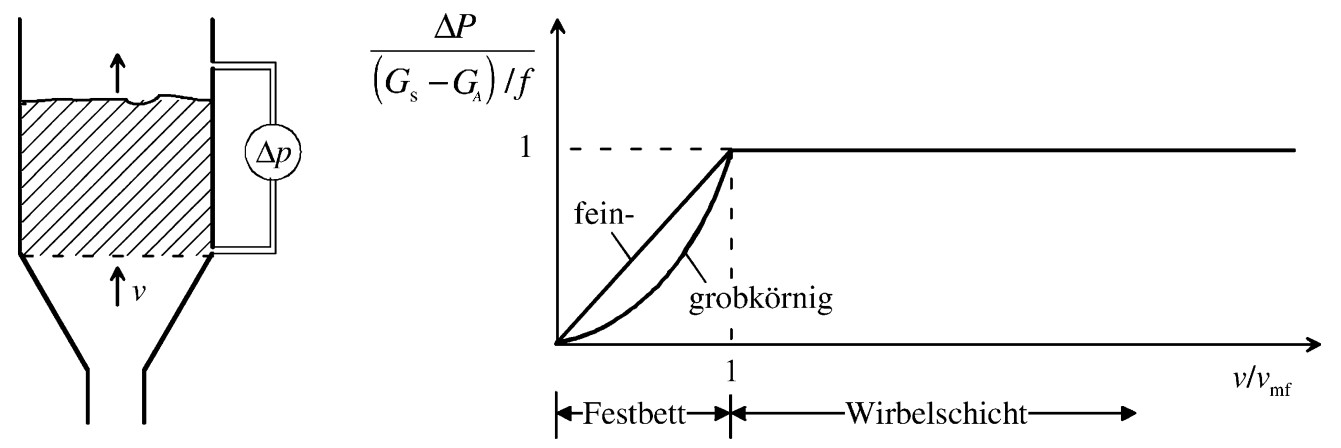
\includegraphics[width=1\textwidth]{Bilder/Lockerungspunkt.jpg}
\vspace{0em}
 \caption[Konstantz des dimensionslosen Drucks, ab dem überschreiten der Lockerungsgeschwindigkeit]{Konstantz des dimensionslosen Drucks, ab dem überschreiten der Lockerungsgeschwindigkeit $v_{\mathrm{mf}}$, in Anlehnung an  \cite[S. 1563]{vdiwaermeatlas2019}}\label{fig:lockerungsgeschwindigkeit}
\end{figure}

\subsubsection{Anmerkung}
 Für tiefgreifendes Wissen zur Berechnung von Wirbelschichten wird auf Fachliteratur, wie dem VDI Wärmeatlas \cite[S. 1561 ff.]{vdiwaermeatlas2019}, verwiesen.





\newpage
\subsection{Signalverarbeitung}

In diesem Abschnitt werden die Grundlagen der Signalverarbeitung erläutert. Im ersten Abschnitt werden nochmals die Grundlagen der Rechnerkommunikation erläutert, gefolgt von dem Unterschied zwischen analogen und digitalen Signalen. Es werden einige Kabelgebundene Schnittstellen, aber auch Schnittstellen die via Funk funktionieren, erläutert.\\


\subsubsection{Vom Bit bis zur \glqq vom Menschen lesbaren\grqq{} Alphanumeric}

Sobald man von digitalen Daten spricht, ist von Bit encodierten, binären Daten die Rede. PC's sind in der Lage, diese Form der Signale direkt zu verarbeiten. In der Abbildung \ref{binary_data_sizes} sind verschiedene Datengrößen binärer Daten aufgezeigt. In der Abbildung variiert die Spanne der Datengrößenlänge von einem Bit bis zu einem Wort bestehend aus 16-Bit. Binäre digitale Daten sind diskret. Ein Bit hat zwei mögliche Zustände, an oder aus, die durch die binären Werte 0 oder 1 sowie den booleschen Ausdrücken \,{\Menlo true} oder \,{\Menlo false} repräsentiert werden können. Die Anzahl, wie viele Bit ein Zeichen (\textit{engl. character}) repräsentiert, kann sich unterscheiden. Häufig wird ein Byte bestehend aus 7 oder 8-{\Menlo Bit} verwendet. In der Abbildung \ref{binary_data_sizes} ist eine ByteLänge von 8-{\Menlo Bit}, häufig auch Oktett genannt, dargestellt. Ein Byte, welches aus 8-Bit besteht, hat 256 mögliche Zustände. Die Hälfte eines (8-Bit) Byte wird\, Nibble genannt \cite[S. 3]{hughes2010real}. Sind Signale ASCII encodiert, beträgt die Byte Länge 7 Bit. Der ASCII Zeichensatz beinhaltet somit 128 (0 - 127) Zeichen. ASCII-Tabellen können alle Zeichen der 7-Bit ASCII Codierung sowie die Zuordnung der dezimalen und hexadezimalen Werte entnommen werden. \\

\bildp{h}{0.6}
{binary_data_sizes.png}
{0em}
{Binary data sizes }
{Binary Data Sizes \cite[S. 3]{hughes2010real} }
{binary_data_sizes}


\paragraph*{Hexadezimal} Zeichen können neben der binärer und der dezimalen Darstellung auch Hexadezimal dargestellt werden. Die Hexadezimale Skala geht von 0 bis 9 gefolgt von A bis F. Die Skala hat somit eine dezimale Ziffernlänge von 16. Ein Nibble kann somit durch eine hexadezimale Ziffer dargestellt werden.\\


\subsubsection{Analoge und digitale Signale}

Möchte man Signale verarbeiten, dann ist zwischen zwei Signaltypen zu unterscheiden. Die reale Welt lässt sich durch ein Kontinuum von Zuständen beschreiben. Elektrische Messgeräte erfassen diese Zustände und erzeugen bspw. eine Spannung. Bei einer kontinuierlichen Messung würden bei einer definierten Frequenz, Signale in Form von Spannung generiert werden. Als Beispiel werfen wir einen Blick auf das Messen einer Temperatur. Bei diesem Beispiel nehmen wir einmal an, dass wir einen Temperaturfühler verwenden, der eine Messgenauigkeit von \SI{0.0001}{\degreeCelsius} besitzt. Bei der Messung der Temperatur von Wasser könnte man eine Gleitkommazahl (floating point number oder kurz float) von \SI{19,2334}{\degreeCelsius} angezeigt bekommen. Bis zur zweiten Messung könnte ein Temperaturausgleich zwischen Umgebung und dem Wasser erfolgt sein, was zu einem anderen Temperaturmesswert von bspw. \SI{12,240}{\degreeCelsius} führen könnte. Analoge Signale sind ein Kontinuum von Signalen. \\

\noindent PC's sind in der Lage digitale Signale sequenziell zu verarbeiten. Ein digitales Signale repräsentiert ein physikalisches Signal, Strom oder Spannung. In der Abbildung \ref{analog_digital_data_input} sind typische Methoden abgebildet, wie Daten eines Messobjekts akquiriert und an einen PC übermittelt werden. Oben im Bild sind vier Schalter zu erkennen, die einen Stromkreis schließen können. Diese Form der Signalübertragung wird diskret genannt. Auf dem Bild sind alle Schalter geöffnet, daher wäre pro Leiter ein binär Wert von 0 zu erwarten. In der Mitte der Abbildung ist ein Bit-serieller Datenstrom, anhand der Rechteckfunktion und den binär Werten, zu erkennen. Im unteren Teil der Abbildung ist ein analoges Signal zu erkennen, welches mittels eines analog zu digital Wandlers die Signale in eines von einem PC interpretierbares Signal wandelt. Die umgewandelten Daten werden mittels paralleler Schnittstelle an einen PC sendet.  

\bild{0.65}
{analog_digital_data_input.png}
{0em}
{Digital and analog data inputs \cite{hughes2010real}}
{Digital and analog data inputs \cite{hughes2010real}}
{analog_digital_data_input}



\subsubsection{Schnittstellen}

Messgeräte verfügen über Schnittstellen, über die Daten- und Steuersignale an andere Komponenten oder einen Messgerätebus erfolgen. An einen Messgerätebus werden Messgeräte (Slaves) und Rechner (Master) angeschlossen. Die Datenübertragung ist entweder Bit- oder Byte-seriell. Der Anschluss eines Messgeräts an einen PC kann über zwei Methoden erfolgen. Messgeräte können über analog Signalausgänge verfügen. Diese Signale müssen in einem analog/digital Wandler in ein digitales Signal gewandelt werden. Das Messgerät kann einen integrierten analog/digital Wandler und digitale Schnittstelle verfügen, über die Signale direkt an einen PC gesendet werden können. Die zwei Methoden können der Abbildung \ref{anschluss} entnommen werden \cite[S. 479]{Busch2015}. Diese analogen Signale müssen mittels einer Messkarte in ein digitales Signal umgewandelt werden, die im Anschluss in einem PC in einer Software weiter verarbeitet werden können. Im folgendem werden zwei Kabelgebundene (USB, RS-232) und zwei Kabellose (Bluetooth und W-LAN) Schnittstellen erläutert.

\bild{1}
{signalverarbeitung_hardware.jpg}
{0em}
{Digitale Schnittstelle oder über Messkarte}
{Anschluss eines Messgerätes an den PC, angelehnt an \cite[S. 479]{Busch2015}) 	\\  \textbf{oben} mit Messkarte, \\ \textbf{unten} mit digitaler Schnittstelle}
{anschluss}

\subsubsection{Verbinder}
\label{sec:verbinder}

Um eine Kommunikation zwischen den Geräten zu ermöglichen, bedarf es physikalischer Schnittstellen. Im Laborumfeld werden die USB Schnittstelle und die DB-9 Schnittstelle besonders häufig angetroffen. In der Abbildung \ref{db9_male} ist ein männlicher DB-9 Stecker abgebildet.

\bild{.5}
{db9_male-female.jpg}
{0em}
{DB-9 pin and socket numbering}
{DB-9 pin and socket numbering \cite{db9-male-female}}
{db9_male}



\subsubsection{Bitserielle Datenübertragung}

Es gibt verschiedene Möglichkeiten Signale, bzw. Daten zu übertragen. Eine Möglichkeit ist die serielle Datenübertragung. Eine genauere Bezeichnung wäre\, Bit-serielle Datenübertragung, denn genau genommen gibt es eine Reihe von\, Bit-seriellen Datenübertragungssystemen, unter anderem jedoch auch die\, Byte-serielle Datenübertragung. \\

\bild{0.6}
{serielle_datenuebertragung.png}
{-0.5em}
{Synchronous serial data communication}
{Synchronous serial data communication \cite[S. 52]{hughes2010real}}
{seriallio}

Des Weiteren gibt es zwei Formen der seriellen Datenübertragung, die synchrone und die asynchrone Datenübertragung. In Abbildung \ref{seriallio} ist eine synchrone Datenübertragung dargestellt. An dem Ausgang \textit{Clock Out} ist zu erkennen, dass das Gerät A den Takt und somit die Austauschrate der Schnittstelle vorgibt.Daten sind nur zum Zeitpunkt der fallenden Flanke des Taktsignals valide. Es ist zu erkennen, dass der Takt stets die Mitte der Bit Position trifft, um mögliche Fehler vorzubeugen. Die \glqq reale\grqq{} Rechteckfunktion ist eine Superposition von Funktion verschiedener Frequenzen, was dazu führt, dass bei aufsteigender Flanke und beim fallen der Flanke ein Einschwingen der Funktion stattfindet, bis sich ein konstanter Wert einstellt (siehe Abbildung \ref{squarefunction}). In der Praxis wird eine asynchrone Bit-serielle Datenübertragung häufiger genutzt. Eine fehlerfreie Kommunikation soll die sogenannte Datenflußsteuerung (\textit{engl. flow control}) übernehmen. Bei asynchroner Datenübertragung existiert somit kein Taktsignal. Bei einer asynchroner Datenübertragung kann der Bit Datenstrom neben der \glqq gewünschten\grqq{} Infromationen, z.B. von einer Messung, noch Datenflußsignale enthalten. Datenflußsignale können physikalische Signale sein. Diese Form der Flußsteuerung nennt sich \textit{Hardware-Handshake}. Eine andere Möglichkeit der Datenflußsteuerung ist der sog. \textit{Software-Handshake}. Die Datenflußsignale sind {\Menlo Startbit}, {\Menlo Stopbit} und {\Menlo Paritätsbit}, die ein Zeichen (\textit{engl. Character}) von einem anderen Zeichen abgrenzt. Zeichen können Buchstaben, Zahlen, Vorzeichen etc. sein, die binär versendet werden (0 oder 1) und beispielsweise ASCII encodiert sind.

\bild{0.65}
{square_waves.png}
{0em}
{Ideal versus real square waves}
{Ideal versus real square waves \cite[S. 5]{hughes2010real}}
{squarefunction}


\subsubsection{RS-232}

Die RS-232 Schnittstelle wurde in den 1960 Jahren von der Electronic Industrial Alliance (EIA) standardisiert. Jedes zu übertragende Zeichen (Zahl, Buchstabe, Sonderzeichen) wird zwischen 5 und 9 Bit codiert, wobei 7 und 8 Bit am gebräuchlichsten sind. Die Trennung von benachbarten Zeichen werden mit \textit{Start-} und \textit{Stopbit} realisiert. Die Übertragungsrate kann zwischen 0,3 Bd und 115,2 kBd betragen. Die Entfernung, die erzielt werden kann, ist stark vom verwendetem Kabel und der Übertragungsgeschwindigkeit abhängig. Es sind Entfernungen bis zu einem Kilometer realisierbar. Die Übertragungsgeschwindigkeit wird Baudrate genannt. Ein Bd entspricht 1 Zeichen pro Sekunde. Ein \textit{Symbol/Character} kann aus einem oder mehreren Bits besteht. Die Übertragungsrate ist somit im Vergleich zu anderen Schnittstellen mit, im Normalfall von einem Bit pro Zeichen, der Übertragungsgeschwindigkeit von 0,3 bis 115,2 kbit/s verhältnismäßig gering, reicht aber für die meisten Messtechnischen Anwendungen aus. Für die Kommunikation mittels RS-232 benötigt man eine sog. Flusssteuerung (engl. \textit{flow control}). Der Sender und der Empfänger müssen sich gegenseitig mitteilen, ob sie sende- oder empfangsbereit sind, um Datenverluste zu vermeiden. Die Signale, die man dafür benötigt, werden~ {\Menlo Handshake-Signale}~genannt. Der {\Menlo Handshake} lässt sich mit physischen Signalen über Steuerleitungen ({\Menlo Hardware-Handshake}) oder über digitale Signale (\textit{Software-Handshake}) realisieren. Die Software-Handshake Signale werden über die TxD Signalleitungen versendet. Für den \textit{Software-Handshake} ist die XON/XOFF und für den \textit{Hardware Handshake} die Datenflußsteuerung mittels CTS/RTS eine gängige Methode \cite[S. 480 f.]{Busch2015}. \\

RS-232 beschreibt Spannungspegel und Timing zwischen der Datenübertragungseinrichtung (DÜE) und Datenendeinrichtung (DEE). Nicht Bestandteil des Standards ist das eigentliche Übertragungsprotokoll, wie die Signale kodiert sind (z.B. ASCII), Fehlererkennung usw.. Solche Parameter müssen zwischen der Datenübertragungseinrichtung und der Datenendeinrichtung ausgehandelt werden \cite{wasistrs232}.



Üblicherweise werden für die Übertragung 9-Polige D-Sub Kabel verwendet, aber RS-232 ist nicht an diese Kabel und Stecker Kombination gebunden. In der AbbildungAbbildung \ref{db9_male} sind alle Signale und die Definition der Signale der DB-9 Schnittstelle aufgelistet. Bei der Verwendung eines Software-Handshake sind nur 3 Signalleitungen notwendig, da die Steuersignale über die Datenleitungen gesendet wird. Für den Datentransfer mittels 9-Poligen D-Sub Kabel (siehe Abbildung \ref{db9_male}), sind somit lediglich die Pins 2 (RxD), 3 (TxD) und 5 (GND) notwendig. Bei der Verwendung eines Hardware-Handshakes werden die Datenleitungen über die Pins 7 (RTS) und 8 (CTS) notwendig \cite{db9}. RS-232 ist eine Volt-basierte Schnittstelle. Der logische Wert wahr ({\Menlo true}) ist dem negativen Volt-Level zugeordnet und der logische Wert falsch ({\Menlo false}) ist dem positiven Volt-Level zugeordnet. Die Spanne der Volt-Spannung ist in RS-232 von +/- 3 V bis +/- 25 V spezifiziert.

\subsubsection{RS-485}

RS-485 ist eine Weiterentwicklung des RS-232 Standards. RS-485 ist ein Bus System, welche bis zu 32 Datensender und Empfänger verbinden kann und wird in der Prozessmess- und Prozessleittechnik angewandt. Es sind Übertragungsgeschwindigkeiten von bis zu 35\,MBit/s mit der Verwendung eines 10 Meter Kabels und 100~KBit/s mit einer Kabellänge von 1200 Meter möglich. Die RS-485 Schnittstelle verfügt über 2 Signalkabel. Die Polarität der beiden Kabel ist gegensätzlich (vergleiche Abbildung \ref{RS-485}). Beide Leitungen können Signale in beide Richtungen senden, jedoch nicht zur gleichen Zeit. Der Signalabgriff ist somit differentiell. Das Signal wird somit nicht gegen Null gemessen, sondern zwischen den zwei Leitern gegensätzlicher Polarität. In Abbildung \ref{RS-485} ist eine 8-Bit asynchrone Datenübertragung via RS-485 zu erkennen. Am Anfang und dem Ende der 8-Bit befindet sich ein Start- und ein Stopbit \cite[S. 222 f.]{hughes2010real}.

\begin{figure}[h!]
\centering
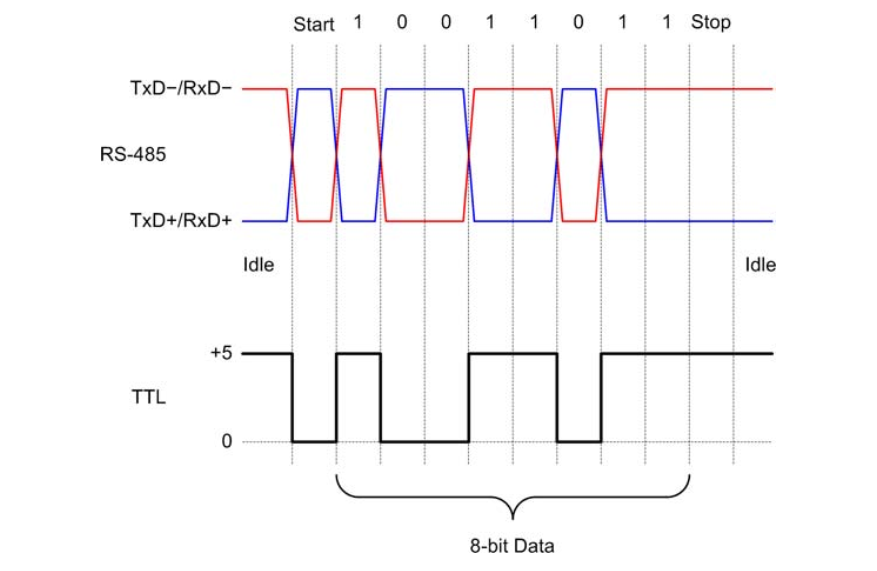
\includegraphics[width=0.7\textwidth]{Bilder/RS-485.png}
\caption{RS-485 signal levels \cite[S. 226]{hughes2010real}}
\label{RS-485} 
\end{figure}

%\bild{1}
%{RS-485.png}
%{0em}
%{RS-485 signal levels}
%{RS-485 signal levels \cite[S. 226]{hughes2010real}}
%{RS-485}

\subsubsection{USB}

Die überbrückbare Länge via USB liegt unter 5 m und liegt somit weit unter der Entfernung, die mit RS-232 möglich sind. USB wurde zwecks Schaffung einer einheitlichen Schnittstelle für alle Arten von PC's Laptops von INTEL entwickelt. USB-Kabel haben vier Leitungen, zwei für die \textit{Bit-serielle} bidirektionale Datenübertragung, eine Leitung für die +5V Versorgungsspannung und eine für das Massepotenzial. An einen USB-Anschluss eines PC's lassen sich theoretisch bis zu 128 Geräte anschließen, da die angeschlossenen Messgeräte durch den USB-Controller im PC mit einer 7-Bit-Adresse adressiert werden. Daraus folgen $2^7=128$ mögliche Messgeräte. Praktisch sind es 127, da die Adresse \glqq Null \grqq \, (000 0000) für die Geräte-Identifizierung genutzt wird. USB verfügt über zwei Eigenschaften, dem \glqq Hot-Plugging\grqq \, und dem \glqq Plug-and-Play\grqq . Dank dem Hot-Plugging ist es vor dem Verbinden eines Geräts mit dem PC nicht notwendig diesen auszuschalten. Dank Plug-and-Play konfiguriert sich die Verbindung selbst. USB 1.0 hat eine Übertragungsgeschwindigkeit von 1,5 bzw. 12 MBit/s, USB 2.0 bis zu 480 MBit/s und USB 3.0 hat eine Highspeedübertragungsrate von 5 GBit/s. Es ist je nach verwendetem Geräte möglich, diese an einer USB-Schnittstelle zu betreiben, die eine geringere Übertragungsrate besitzen als die USB-Schnittstelle des PC's.

\subsubsection{Bluetooth}
\label{sec:bluetooth}

Bluetooth ist eine kabellose Datenübertragungsmethode via Funk. Der Frequenzbereich ist zwischen 2,402 bis 2,480 GHz. Die Übertragungsdistanz beträgt ca. 10 m mit einer Übertragungsgeschwindigkeit von 2,1 MBit/s für die Spezifikation \textit{Bluetooth 2.0 + EDR} (Enhanced Data Rate) \cite[S. 481 f.]{Busch2015}.
Bluetooth 2.0 + EDR ist 2004 auf dem Markt erschienen. Bluetooth 4.2 Smart ist 2014 mit Einführungen von wichtigen Funktionen für das Internet der Dinge (IoT) erschienen. Bluetooth 5 (2017) ist die aktuellste Version und hat IoT im Fokus. Bluetooth 5 unterstützt Übertragungsraten von 2 MBit/s und einer Reichweite von maximal 250 m \cite{bt5}.\\

Drahtlose IoT- Lösungen nehmen in der produzierenden Industrie an Bedeutung zu. Da kabellose Netzwerke beim Aufbau von neuen Fertigungslinien flexibler sind als kabelgebundene Netzwerke, ist Bluetooth im Rahmen von Industrie 4.0 eine bedeutende Schnittstelle. Bluetooth Mesh Networking wurde unter anderem für industrielle drahtlose Sensornetzwerke konzipiert (WSN). Mit diesem Standard ist es möglich viele Geräte und Sensoren in einem Bluetoothnetzwerk kommunizieren zu lassen. Jedes Gerät wird \glqq Knoten\grqq \, genannt \cite{bti40}.

\paragraph*{Sicherheit: Mesh-Vernetzung per Bluetooth \cite{bti40}}

Die Netzwerksicherheit bei produzierenden Betrieben ist nicht verhandelbar. Die Sicherheit bei der Verwendung von Bluetooth, soll durch die sog. Mesh-Vernetzung gewährleistet werden. Die Informationssicherheit soll durch ein Schichtenmodell erreicht weden, dass auf voneinander getrennten Sicherheitsschlüssel basiert:

\paragraph*{Netzwerkschlüssel (NetKeys)} gelten für alle Nachrichten im Netzwerk, damit die Knoten sicher miteinander kommunizieren.

\paragraph*{Anwendungsschlüssel (AppKeys)} schützen Nachrichten zu bestimmten Anwendungen wie Klimaanlage, Beleuchtung oder physische Sicherheit.

\paragraph*{Geräteschlüssel (DevKey)} ermöglichen das Einrichten und Konfigurieren eines Knotens, um neue Geräte zum Netzwerk hinzuzufügen.

\subsubsection*{WLAN}

WLAN ermöglicht die Datenübertragung via Funk, ermöglicht jedoch eine signifikant höhere Übertragungsgeschwindigkeit und Übertagungsreichweite als Bluetooth. Mit der technischen Lösung 802.11 ist eine Gruppe von Standards für Funknetzwerke des Institute of Electrical and Electronics Engineers (IEEE) entwickelt worden. 

\subsubsection{Verarbeitung digitaler Signale in Labview}

Jeff Kodosky et al. hat in Zusammenarbeit mit der University of Texas die Programmiersprache G und die dazugehörige Enwicklungsumgebung LabVIEW entwickelt. 

LabVIEW stellt zum umsetzen spezieller Anwendung spezifische Werkzeuge und Modelle bereit. Das Ziel war es ein Tool zu entwickeln, wodurch Menschen mit unterschiedlichem know-how im Programmieren befähigt werden maßgeschneiderte Programme grafisch generieren zu können, da sich im Laborumfeld Versuchsaufbauten und somit auch Messungsaufgaben und Prozessabläufe schnell ändern. Diese Programme nennen sich \textit{Virtual Instruments} (VI) und emulieren physische Instrumente. Diese Programmiersprache setzt sich aus zwei Programmiermethoden zusammen, dem strukturorientiertem Programmieren und der datenstromorientierten Programmierung  \cite{kodosky}. Zu den strukturorientierten textbasierten Programmiersprachen gehören unter anderem \textit{C++, Java} und {\Menlo Python}. Programmiersprachen, die strukturorientiert arbeiten, befolgen auf der untersten Funktionsebene folgende drei Kontrollstrukturen \cite{structured}:

\begin{enumerate}
\singlespacing
\item Sequenzielle Abarbeitung von Programmanweisungen
\item Verzweigung innerhalb Programmabschnitte (if/when/else)
\item Iterationen/Schleifen
\end{enumerate} 

\bildp{h!}{0.8}
{blockdiagramm_frontpanel.png}
{-1em}
{Beispiel für ein Blockdiagramm und das zugehörige Frontpanel}
{Beispiel für ein Blockdiagramm und das zugehörige Frontpanel \cite{blockdiagramm_frontpanel}}
{blockdiagramm_frontpanel}

Viele Messobjekte generieren kontinuierliche Datenströme. Die datenstromorientierte Programmiermethode ist bei dieser Art von Messobjekt die Methode der Wahl, daher liegt der Programmiersprache G im wesentlichen das Datenflusskonzept zugrunde. G ist eine effiziente Programmiersprache, die die Kommunikation mit den Geräten, die Visualisierung von Daten und deren Analyse ermöglicht. Mittels LabVIEW lassen sich Programme grafisch mittels drag and drop entwickeln. LabVIEW Programme setzen sich aus interaktiven Front Panels und dem Programm in Form von Blockdiagrammen zusammen \cite{kodosky}. Das Front Panel ist die Programmoberfläche des Programms, womit das Programm angewendet wird. In Abbildung \ref{blockdiagramm_frontpanel} sind Frontpanel und Blockdiagramm eines einfachen Programms dargestellt.

%\subsection{Datenverwaltung}

Für Für die Verwaltung von Daten bieten sich Datenbank Management Systemen (DBMS) an. DBMS, die in Laboren angewendet werden nennen sich Labor Informations Management Systeme (LIMS). In vielen Fällen werden LIMS in Kombination mit Elektronischen Labor Notebooks (ELN) verwendet. LIMS sind Datenbanksysteme, die Daten bzw. Datensätze verschiedener Routineinstanzen (z.B. Waren/Probeneingang, Prüfungsdurchführende Labormitarbeiter etc.) relational verknüpfen. Die LIMS verwalten in Laboren sämtliche Daten entlang der Laborroutinen, vom Proben Eingang, bis hin zur Qualitätsfreigabe. Die ELN Applikationen dienen dem Laborpersonal, um beispielsweise Erkenntnisse aus Versuchsreihen zu dokumentieren. ELN Systeme können in LIMS integriert werden, um redundante Dateneingaben zu reduzieren oder um sie zu eliminieren. Des Weiteren existieren neben dem relationalen Datenbanktyp noch weitere Datenbanktypen. \\

\subsubsection{PERA}

Das Purdue Enterprise Reference Architecture (PERA) Modell beschreibt Automatisierungsnetze und unterteilt diese in fünf Ebenen, bzw. \glqq Level\grqq{} (siehe  Abbildung \ref{pera_modell}. Die oberen zwei Hierarchieebenen sind in vielen Unternehmen von den Ebenen 3 bis 0 aus sicherheitstechnischen Gründen physisch voneinander getrennt. Die oberen zwei Ebenen werden IT-Ebene und die unteren vier sind der Industrial Control Systems (ICS; deutsch: industrielle Steuerungssysteme, Automatisierungssysteme) Ebene zugeordnet \cite{ics_kompendium}.

\begin{figure}
\begin{center}
\caption{PERA Model \, \cite{pera_modell}}
\vspace{1em}
\begin{tikzpicture}[
	scale=0.75,
	start chain=1 going below, 
	start chain=2 going right,
	node distance=1mm,
	desc/.style={
		scale=0.75,
		on chain=2,
		rectangle,
		rounded corners,
		draw=black, 
		very thick,
		text centered,
		text width=8cm,
		minimum height=12mm,
		fill=blue!30
		},
	it/.style={
		fill=blue!10
	},
	level/.style={
		scale=0.75,
		on chain=1,
		minimum height=12mm,
		text width=2cm,
		text centered
	},
	every node/.style={font=\sffamily}
]

% Levels
\node [level] (Level 5) {Level 5};
\node [level] (Level 4) {Level 4};
\node [level] (Level 3) {Level 3};
\node [level] (Level 2) {Level 2};
\node [level] (Level 1.5) { };
\node [level] (Level 1) {Level 1};
\node [level] (Level 0) {Level 0};

% Descriptions
\chainin (Level 5); % Start right of Level 5
% IT levels
\node [desc, it] (Archives) {Archives/File Servers};
\node [desc, it, continue chain=going below] (ERP) {ERP/Finance/Messaging};
% ICS levels
\node [desc] (Operations) {Operations Management/Historians};
\node [desc] (Supervisory) {Supervisory Controls};
\node [desc, text width=3.5cm, xshift=2.25cm] (PLC) {PLC/RTU IP Communication};
%\node [desc, text width=3.5cm, xshift=-4.5cm] (SIS) {Safety Instrumented Systems};
\node [desc, xshift=-2.25cm] (SIS) {Safety Instrumented Systems};
\node [desc] (IO) {I/O from Sensors};

\end{tikzpicture}
\label{pera_modell}
\end{center}
\end{figure}


\paragraph{Level 4} Es ist zu erkennen, dass das Level 4 dem Enterprise Level entspricht. Softwarelösungen dieser Ebene werden Enterprise Ressource Planning (ERP) Systeme genannt. Der Enterprise Ebene sind beispielsweise Systeme der Buchhaltung und der Personalabteilung zugeordnet. Zwischen dem Level 4 und dem Level 3 befindet sich die Schnittstelle zum Anlagennetz.

\paragraph{Level 3} Das operative Management ist dem Level 3 zugeordnet. Auf diesem Level findet die Betriebsführung, wie z.B. die Produktionsplanung, Produktversand etc. statt.

\paragraph{Level 2} Dem Level 2 ist die spezifische Prozessführung (Supervisory Control) zugeordnet. Ein Absturz von Systemen diesen Levels haben keinen Einfluss auf die Produktion, da die Datenverarbeitung diesen Levels nicht in Echtzeit verläuft. Die Level 2, 1 und 0 unterscheiden sich z.T. gravierend, je nach betrachtetem Unternehmen.

\paragraph{Level 1} Level 1 ist das Basic Control. Daten und Signale sind auf dieser Ebene in Echtzeit. Die Ausführung und Steuerung physischer Prozesse geschieht auf dieser Ebene. Anlagen werden hier gesteuert und über Sensoren geregelt.

\paragraph{Level 0} Level 0 ist die sogenannte Feldebene. Anlagen und Sensoren sind dieser Ebene zugeordnet.



\subsubsection{ISA-S95}

Unternehmen sind sozio-ökonimische Systeme. Um global Wettbewerbsfähig zu bleiben ist Flexibilität und das anwenden effizientere Methoden als Unternehmen aus Billiglohnländern ein muss. Um das zu gewährleisten, ist ein System notwendig, welches die gesamte Wertschöpfungskette abbilden kann. Ein effizienter Datenfluss zwischen verschiedenen Unternehmenssystemen wie ERP oder MES ermöglicht der ISA-95 Standard. ISA-S95 definiert Terminologie und einheitliche Modelle, um die Kommunikation zwischen sämtlicher Kontroll- und Unternehmenssystemen zu verbessern. Die Aktivitäten innerhalb eines Unternehmens werden nach dem PERA Modell unterteilt. Die Level 0,1 und 2 decken damit die Aktivitäten der Produktion ab.

Ein Unternehmen kann man hierarchisch unterteilen. Die International Society of Automation, kurz ISA hat 1995 einen Standard etabliert der Terminology und ein Model für den effizienten Datenaustausch zwischen Systemen verschiedener Hierarchiestufen ermöglicht. Der Name des Standards ist ISA-S95. Der ISA-S95 Standard bedient sich der Purdue Enterprise Reference Architecture (PERA). 

ISA-S95 besteht aus fünf Parts. Der erste Part besteht aus Terminologie und Model für e

Um eine effiziente Unternehmensführung zu gewährleisten werden Tools verwendet. Unternehmen nutzen eine Vielzahl von Software Lösungen und Systemen. 

\subsubsection{Datenbanken}

\paragraph{XML}




\newpage
\subsection{Datenverwaltung}

Die analogen Signale, die von einem Messobjekt akquiriert (\textit{engl. acquisition}), in digitale Signale umgewandelt und in der Signalverarbeitung aufbereitet werden, sollen in den meistens Fällen weiterverwendet werden. Die Verwendung dieser Daten kann je nach Anwendungsfeld in Echtzeit oder zu einem beliebigen Zeitpunkt erfolgen. Der Zeitpunkt der Wiederverwendung ist bei der Wahl der Technologie zur Verwaltung der Daten zu beachten. Welche Art von Daten gespeichert werden sollen determiniert ebenfalls die Wahl der Lösung. Sollen z.B. nur Zahlen oder Strings abgespeichert werden oder ist auch die Speicherung von Audio, Bild oder Videos erwünscht oder in Betracht zu ziehen. Des Weiteren unterscheiden sich Softwarelösungen darin, ob die Daten von einem Anwender oder von einer Software "autonom" abgerufen und verwendet werden sollen \cite[S. 2 ff.]{sqlnosql}. \\

In diesem Abschnitt werden Informationsmanagementsysteme, das PERA Modell zur Strukturierung von Automatisierungsnetzen, welches Teil des ISA-95 \textcolor{blue}{\underline{S}}tandards ist sowie ISA-\textcolor{blue}{\underline{S}}95 erläutert.

% bieten sich Datenbank Management Systemen (DBMS) an. DBMS, die in Laboren angewendet werden nennen sich Labor Informations Management Systeme (LIMS). In vielen Fällen werden LIMS in Kombination mit Elektronischen Labor Notebooks (ELN) verwendet. LIMS sind Datenbanksysteme, die Daten bzw. Datensätze verschiedener Routineinstanzen (z.B. Waren/Probeneingang, Prüfungsdurchführende Labormitarbeiter etc.) relational verknüpfen. Die LIMS verwalten in Laboren sämtliche Daten entlang der Laborroutinen, vom Proben Eingang, bis hin zur Qualitätsfreigabe. Die ELN Applikationen dienen dem Laborpersonal, um beispielsweise Erkenntnisse aus Versuchsreihen zu dokumentieren. ELN Systeme können in LIMS integriert werden, um redundante Dateneingaben zu reduzieren oder um sie zu eliminieren. Des Weiteren existieren neben dem relationalen Datenbanktyp noch weitere Datenbanktypen. \\

\subsubsection{Informationsmanagementsysteme}
\label{sec:Informationsmanagementsysteme}

Für strukturierte, leicht abrufbare Daten bieten sich Informationsmanagementsysteme (IMS) an. Im Rahmen großer Datenmengen in der Privatwirtschaft ist der Begriff Datawarehouse zu nennen, darauf wird im Rahmen dieser Arbeit nicht weiter eingegangen. IMS können verschiedenste Informationen miteinander Verknüpfen. Die automatisierte Erhebung von Kennzahlen ist damit einfach zu erreichen. Des Weiteren wird eine schnelle Verfügbarkeit der Informationen (die sich im IMS befinden) für Anwender und Software durch gut programmierbare Abfragen (\textit{engl. Querys}) ermöglicht. Der Nachteil besteht darin, dass die Daten, die das IMS erhebt bzw. dem IMS zugeführt werden sollen im Vorwege definiert werden müssen. Folglich kann daraus ein Daten bzw. Informationsverlust entstehen \cite[S. 2 ff.]{sqlnosql}. Die Daten und Informationen die heute noch als unwichtig gelten, können morgen eine signifikante Relevanz in Bezug auf die Wettbewerbsfähigkeit eines Unternehmens haben \cite{bigdata}. IMS müssen von Administratoren (Spezialisten) instand gehalten werden, wodurch Kosten entstehen. Nutzt man einen Dienstleister, fallen i.d.R nur gut kalkulierbare Fixkosten an.  Wird sich für ein betriebsinternes IMS entschieden, entstehen Fixkosten und variable Kosten (sobald Updates oder Modifikationen oder der gleichen an der IMS Struktur anfallen). Der Trend von Unternehmen in Bezug auf IMS geht weg von betriebsinterner Datenverwaltung in Richtung der Nutzung von Dienstleistern wie Amazon und co.. Vor- und Nachteile von Informationsmanagementsystemen können der Tabelle \ref{tab:vor_nach_ims} entnommen werden.

\begin{table}[h!]
\caption{Vor- und Nachteile von Informationsmanagementsystemen \cite[S. 2 ff.]{sqlnosql}}\label{tab:vor_nach_ims}
\begin{center}
\begin{tabular}{l|l}
Vorteile & Nachteile\\ \toprule
\makecell[l]{\textbullet \, schnelle Verfügbarkeit von Information\\ \hspace{0,19cm} für Software und Anwender  } &  \makecell[l]{\textbullet \,  potentieller Informationsverlust von \\ \hspace{0,19cm} vermeintlich unwichtigen Daten}\\ 
\textbullet \,  Kennzahlengenerierung & \textbullet \,  Wartungs-/Instandhaltungskosten \\
\textbullet \,  Informationsverknüpfung   &  \\
\end{tabular}
\end{center}
\end{table}

Informationen sind in vielen Branchen entscheidend für die Konkurrenzfähigkeit eines Unternehmens. Informationen können sich aus Daten destillieren lassen und sind in dem derzeitigen digitalem Zeitalter von großer Bedeutung. Neben den konventionellen Produktionsfaktoren, Arbeit, Boden und Kapital könnten Informationen bzw. Wissen somit hinzugezählt werden. Produktionsfaktoren sind Wirtschaftsgüter die genutzt werden, um Leistungen erbringen zu können. Produktionsfaktoren sind Ressourcen die geplant, gesteuert, überwacht und kontrolliert werden müssen. Wird sich dafür entschieden Wissen bzw. Daten als einen Produktionsfaktor zu betrachten, wird das Datenmanagement zur Führungsaufgabe. 
Die Entscheidung Informationen als Produktionsfaktor anzuerkennen wirkt sich wie folgt aus \cite[S. 2 f. ]{sqlnosql}:\pagebreak

\noindent \begin{itemize}[leftmargin=*,labelsep=-\mylen]
\item \textbf{Entscheidungsgrundlage:} Für viele Entscheidungen dienen Daten als Grundlage, somit sind sie für alle Organisationsfunktionen von Bedeutung. 
\item \textbf{Qualitätsanspruch:} Verfügbarkeit, Korrektheit und Vollständigkeit sind maßgeblich für die Qualität der Daten. 
\item \textbf{Investitionsbedarf:} Die Speicherung, Verwaltung, und ggf. Aufbereitung von Daten erzeugen Kosten und erfordern demnach Kapital.
\item \textbf{Integrationsgrad:} Der Integrationsgrad der Daten bestimmt die Verknüpfbarkeit von Informationen zwischen den Aufgabengebieten und -träger jeder Organisation.
\end{itemize}

In der Abbildung \ref{fig:Informationssystem} ist das Schema eines Informationsmanagementsystems dargestellt, welches mit einem Kommunikationsnetz bzw. mit dem Internet verbunden ist. Informationssysteme können eine Wissensbank, Methodenbank und/oder Datenbank enthalten. Auf die Methoden- und Wissensbank wird im Rahmen dieser Arbeit nicht weiter eingegangen \cite[S. 2 f. ]{sqlnosql}.

\begin{figure}[h!] %[htbp!] 
\centering
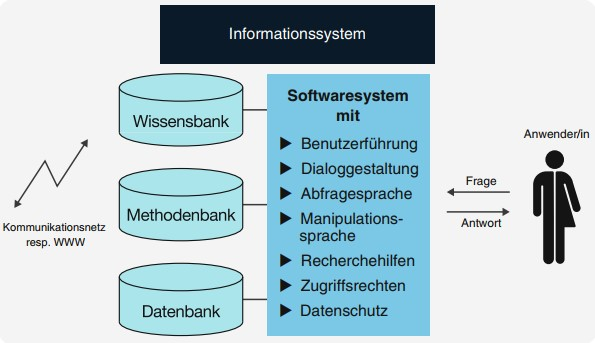
\includegraphics[width=0.7\textwidth]{Bilder/Informationssystem.jpg}
 \vspace{0em}
 \caption[Informationssystem]{Architektur und Komponenten eines Informationssystems  \cite[S. 3]{sqlnosql}}\label{fig:Informationssystem}
\end{figure}

\paragraph*{Datenbankmanagementsysteme}
Ein Datenbanksystem (\textit{engl. database management system}, DBMS) dient der Speicherung und Abfrage von Daten und besteht aus einer Speicher- und Verwaltungskomponente. Die Speicherungskomponente umfasst alle Daten, welche in einer organisierten Form abgespeichert werden sowie deren Beschreibung. Um die Daten und Informationen verändern und auswerten zu können bedarf es einer Abfrage- und Manipulationssprache, die die Verwaltungskomponente darstellt. Die Zugriff- und Bearbeitungsrechte werden ebenfalls von der Verwaltungskomponente verwaltet. In der Praxis kommen häufig SQL-Datenbanken (\textit{Structured Query Language}) zum Einsatz. Sind Datenbestände heterogener Natur und müssen in Echtzeit verarbeitet werden, dann sind SQL-Datenbanken ungeeignet. Für solche Anwendungsfälle bieten sich Lösung im Rahmen von Big Data oder Hybridlösungen an. Datenverwaltungslösungen im Rahmen von Big Data sind No-SQL Datenbanken (not only SQL-Datenbanken) \cite[S. 2 f.]{sqlnosql}.

\paragraph{SQL-Datenbanken}

SQL-Datenbanken sammeln Daten bzw. Informationen in Tabellen. Diese Tabellen können miteinander in Beziehung stehen. Aus diesem Grunde werden SQL-Datenbanken auch relationale Datenbanken genannt. In der Abbildung \ref{fig:tabellengeruest} ist eine Tabelle abgebildet, die den Namen MITARBEITER trägt. Tabellen bestehen aus Schlüsselmerkmalen und Attributen. Schlüsselmerkmale dienen der \textbf{eindeutigen} Identifikation. Ein Merkmal oder Attribut ordnet jedem Eintrag einer Tabelle einen bestimmten Datenwert aus einem vordefinierten Wertebereich (\textit{engl. domain}) zu. Somit kann jeder Mitarbeiter, der eindeutig mit der Mitarbeiter ID identifiziert werden kann, mit Namen und Ort eingetragen und in der Tabelle gefunden werden. Als Schlüsselmerkmal bietet sich demnach die Mitarbeiter ID (\emph{M\#}) an. Die minimale Schlüsselkombination wird in diesem Beispiel durch den \textbf{Identifikationsschlüssel} \emph{M\#} repräsentiert. Schlüsselkombinationen haben einen \textbf{Minimalitätsanspruch}. In diesem Fall darf kein Schlüssel oder Kombination gestrichen werden, ohne dass die eindeutige Identifikation verloren geht. Ein Schlüssel ist mit den Forderungen der \textbf{Minimalität} und \textbf{Eindeutigkeit} vollständig charakterisiert. Datenwerte dürfen mehrfach vorkommen, siehe Abbildung \ref{fig:auspraegungen}. Eine komplette Zeile einer Tabelle wird Datensatz bzw. Tupel genannt und beschreibt ein Objekt in einer Tabelle (ID, Name, Adresse usw.) \cite[S. 3 ff.]{sqlnosql}.\\

Die Anzahl an Spalten und Zeilen ist unbegrenzt. Die Benennung von Tabellen und Merkmalen sowie der Identifikationsschlüssel bzw. Schlüsselkombination muss eindeutig sein. Mathematisch ist eine Relation R, die diesen Anforderung erfüllt, eine Teilmenge aus dem kartesischen Produkt von Wertebereichen $\mathrm{R} \subseteq \mathrm{D}_1\cdot \mathrm{D}_2\cdot...\,\mathrm{D_n}$ mit $\mathrm{D_i}$ als Wertbereich des i-ten Merkmals \cite[S. 3 ff.]{sqlnosql}.



\begin{figure}[h!] % Relationsmodell
\centering
%\hspace{0em}
\captionsetup{position=bottom}
     \subfloat[][Tabellengerüst\label{fig:tabellengeruest}]{%
       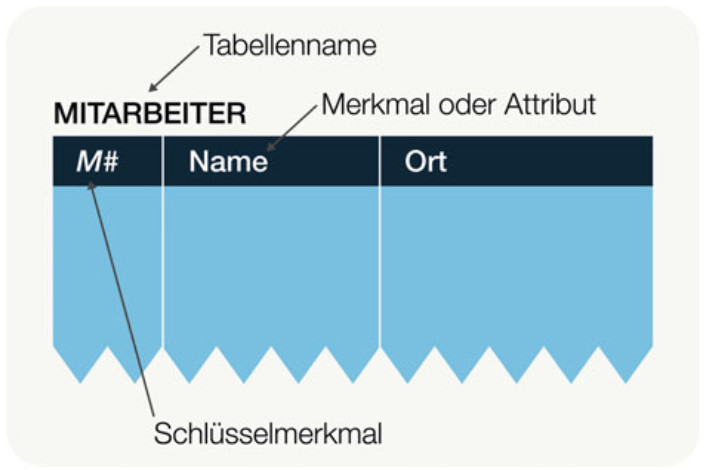
\includegraphics[width=0.40\textwidth,]
       {Bilder/relationstabelle.jpg} %{Bilder/LabVIEW_serialport/}
     }
\hspace{1,5em}%
%\hfill     
    \subfloat[][Ausprägungen\label{fig:auspraegungen}]{%
       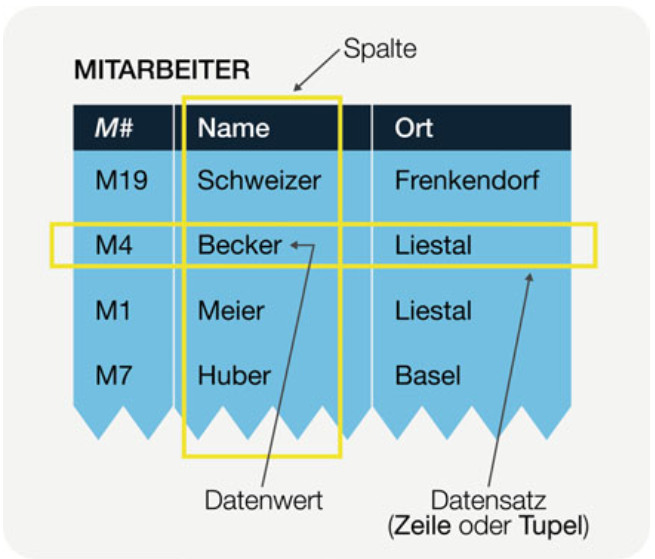
\includegraphics[width=0.40\textwidth]
      {Bilder/relationstabelle_gefuellt.jpg}
      }
\caption[Relationenmodell: Tabellengerüst und Ausprägung einer SQL-Tabelle]{Relationenmodell: Tabellengerüst und Ausprägung einer am Beispiel einer \mbox{MITARBEITER Tabelle}}
\label{fig:relationenmodell}
   \end{figure} 

Ein Tupel r ist demnach ($\mathrm{r} = \mathrm{d}_1 ,\, \mathrm{d}_2 ,...,\,\mathrm{d_n}$). Tupelredundanzen sind aufgrund des Teilmengenbegriffs nicht erlaubt, d.h. $\mathrm{R}=\{\mathrm{r}_1 , \, \mathrm{r}_2 , \, ... , \,\mathrm{r_n}\}$

\footnotesize \singlespacing
\noindent \textbf{Anmerkung:} Beim programmieren sind Tupel unveränderbare, schreibgeschützte Arrays!
\normalsize \onehalfspacing

\subparagraph*{Strukturierte Abfragesprache SQL}

\textit{SQL} (\textit{Structured Query Language}) ist eine \textit{deskriptive} von ANSI und ISO genormte Abfrage- und Manipulationssprache für Tabellen. In der Abbildung \ref{fig:sql} ist ein Beispiel einer Abfrage. unter der Tabelle MITARBEITER ist die Abfrage in natürlicher Sprache (<<Selektiere den ... wohnen>>) zu sehen. Das Resultat der Abfrage sollen alle Namen/Personen die den Wohnort Liestal angegeben haben sein. Die Formulierung einer Abfrage genügt dem Schema SELECT-FROM-WHERE. Eine Formulierung in SQL sieht wie auf Abbildung \ref{fig:sql} zu erkennen folgt aus \cite[S. 6 ff.]{sqlnosql}:

\begin{table}[h!]
\centering
\begin{tabular}{r|l}
SELECT & Name \\
FROM & MITARBEITER \\
WHERE & Ort = 'Liestal' \\
\end{tabular}
\end{table}

\begin{figure}[] %SQL 
\centering
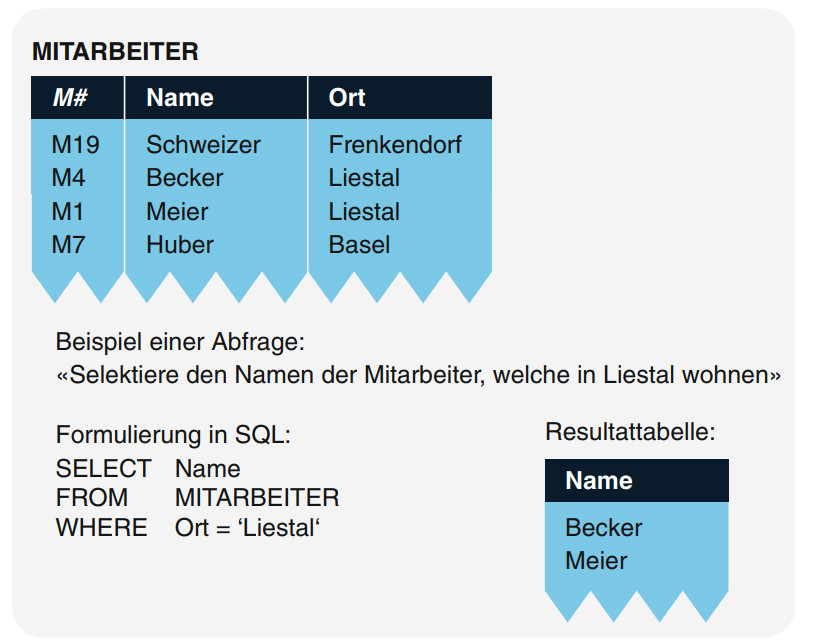
\includegraphics[width=0.6\textwidth]{Bilder/SQL.jpg}
\vspace{0em}
 \caption[]{Formulierung einer SQL Abfrage}\label{fig:sql} %\ref{}
\end{figure}

Für tiefgreifendes Wissen bezüglich SQL-Datenbanken muss auf Fachliteratur wie \cite{sqlnosql} verwiesen werden.

\paragraph{Big Data}

Datenbestände die mit den herkömmlichen technischen Lösungen (SQL-Datenbanken) aufgrund vom sehr hohem Datenvolumen, einer heterogenität von Daten und der Notwendigkeit diese in Echtzeit bei einer hinreichender Geschwindigkeit zu verarbeiten nicht mehr zu handhaben sind, werden unter dem Begriff von \textit{Big Data} zusammengefasst. Der Begriff \textit{Big Data} ist nicht klar definiert. Datenspezialisten wie die Gartner Group definiert Big Data in ihrem \emph{\glqq Information Technology Glossary\grqq{}}mit dem Vorhandensein von mindestens drei \texttt{V}'s \cite[S. 11]{sqlnosql}:\\

\glqq \textbf{Big data} is high-\texttt{v}olume, high-\texttt{v}elocity and/or high-\texttt{v}ariety information assets that demand cost-effective, innovative forms of information processing that enable enhanced insight, decision making, and process automation.\grqq, \cite{BigData}. \\

Wie bereits in Kapitel \ref{sec:Informationsmanagementsysteme} erläutert sind Informationen entscheidend für die Konkurrenzfähigkeit von Unternehmen in vielen Branchen. Die Gartner Group bezeichnet Informationen sogar als \textit{Vermögenswert} oder \textit{Informationskapital} (\textit{engl. information asset}).

Eine Präzisierung der drei \texttt{V}'s laut\cite{sqlnosql} ist folgende: 

\begin{itemize}[leftmargin=*,labelsep=-\mylen]
\item \textbf{Velocity}: Datenströme sollen in Echtzeit analysiert und ausgewertet werden können,
\item \textbf{Volume}: Umfangreiche Datenbestände bis zum Zettabytebereich (1 Zettabyte $+10^{12}$ GB),
\item \textbf{Variety}: Strukturierte, semi-strukturierte und unstrukturierte Multimedia-Daten (Texte, Bilder, Grafiken, Audio Videos) sollen gespeichert werden können.
\end{itemize}

Zuletzt bleibt noch die Information als \texttt{V}ermögenswert (\textit{engl. \texttt{v}alue}) und die Aussagekraft bzw. Wahrhaftigkeit (\textit{engl. \texttt{v}eracity}) der Daten bzw. Auswertungsergebnisse. Da die Daten im Rahmen von \textit{Big Data} heterogener Natur in Art und Präzision sind, müssen spezielle Algorithmen für hinreichende Ergebnisse angewendet werden.  


\subsubsection{PERA-ICS Modell}

Die \textbf{P}urdue \textbf{E}nterprise \textbf{R}eference \textbf{A}rchitecture (PERA) wurde Anfang 1990 entworfen, um Automatisierungsnetze zu beschreiben und zu unterteilen. Des Weiteren dient es unter anderem dazu, den Schutz von industriellen Steuerungs- und Automatisierungsnetze, vor Hackern, zu gewährleisten. Klassisch wird das ICS-Modell (\textbf{I}ndustrial \textbf{C}ontrol \textbf{S}ystem) in fünf Ebenen (\textit{engl. Level}; siehe Abbildung~\ref{pera_modell}) unterteilt. Die oberen zwei Hierarchieebenen sind, gemäß PERA-ICS, von Level 3 bis \textcolor{black!60}{Level 0}, aus sicherheitstechnischen Gründen, physisch voneinander getrennt \cite[S. 15 ff.]{ics_kompendium}. Auf die Funktionen und Komponenten, wie z.B. HMI/BuB (\textbf{H}uman-\textbf{M}achine-\textbf{I}nterface = \textbf{B}edienung \textbf{u}nd \textbf{B}eobachtung), \textit{\textbf{M}anufacturing \textbf{E}xecution \textbf{S}ystem} (MES) oder \textit{\textbf{M}anufacturing \textbf{O}perations \textbf{M}anagement} (MOM) und \textit{\textbf{E}nterprise \textbf{R}essource \textbf{P}laning} (ERP) Systeme usw., die auf den Leveln vorhanden sind, wird im Rahmen dieser Arbeit nicht eingegangen.

\begin{figure} % PERA Model
\begin{center}
\begin{tikzpicture}[
	scale=0.75,
	start chain=1 going below, 
	start chain=2 going right,
	node distance=1mm,
	desc/.style={
		scale=0.85,
		on chain=2,
		rectangle,
		rounded corners,
		draw=black, 
		very thick,
		text centered,
		text width=12cm,
		minimum height=12mm,
		fill=blue!30
		},
	it/.style={
		fill=blue!10
	},
	level/.style={
		scale=0.85,
		on chain=1,
		minimum height=12mm,
		text width=2cm,
		text centered
	},
	every node/.style={font=\sffamily}
]

% Levels
\node [level] (Level 5) {Level 5};
\node [level] (Level 4) {Level 4};
\node [level] (Level 3) {Level 3};
\node [level] (Level 2) {Level 2};
\node [level] (Level 1.5) { };
\node [level] (Level 1) {Level 1};
\node [level] (Level 0) {\textcolor{black!60}{Level 0}};

% Descriptions
\chainin (Level 5); % Start right of Level 5
% IT levels
\node [desc, it] (Archives) {Produktionsführung: ERP, Finanzen uvm.};
\node [desc, it, continue chain=going below] (ERP) {Betriebssführung: MES, Engineering/Planung uvm.};
% ICS levels
\node [desc] (Operations) {Einrichtung zur Prozessführung};
\node [desc] (Supervisory) {Realtime Prozessführung};
\node [desc, text width=3.5cm, xshift=4.25cm] (PLC) {Kommunikation z.B. via RS-232};
%\node [desc, text width=3.5cm, xshift=-4.5cm] (SIS) {Safety Instrumented Systems};
\node [desc, xshift=-4.25cm] (SIS) {Prozessführung im Feld};
\node [desc] (IO) {Materieller Produktionsprozess};
\end{tikzpicture}

\vspace{0,5em}
\caption[]
{ICS-PERA Model, angelehnt an der Grafik des Bundesamtes für Sicherheit in der Informationstechnik des ICS-Kompendiums (vgl. Abbildung \ref{fig:Hierarchische_Gliederung_gem_ICS} im Anhang ; \cite[S. 18]{ics_kompendium})}
\label{pera_modell}
\end{center}
\end{figure}

\paragraph*{\textcolor{black!60}{Level 0}} Gemäß des ICS-Kompendiums des Bundesamtes für Sicherheit in der Informationstechnik, befindet sich vor dem Level 1 der \textbf{materielle Produktionsprozess} \cite[S. 18]{ics_kompendium}. In dem ICS-Kompendium ist es nicht gelabelt, doch in vielen anderen Quellen wird dieses mit \textcolor{black!60}{Level 0} deklariert.

\paragraph*{Level 1} Level 1 ist die \textbf{Prozessführung im Feld} (\textit{engl. Basic Control}). Daten und Signale werden auf dieser Ebene in Realtime generiert und erfasst. Die Ausführung der Steuer- und Regelung physischer Prozesse geschieht auf dieser Ebene. Als Beispiele, für die Infrastruktur dieser Ebene , können Remote I/O (ggf. mit Signalvorverarbeitung, dann spricht man von RTU), Interface-Bausteine zur Signalkonditionierung, Switches bei Verwendung von Feldbus Lösungen genannt werden \cite[S. 18]{ics_kompendium}.

\paragraph*{Level 2} Komponenten der \textbf{Realtime Signalverarbeitung}, im Sinne der Darstellung der automatisierten Funktionen sind dem Level 2 zugeordnet. Beispiele können Zustände der Komponenten der Feldebene sein. Als Beispiele können Füllstände, Motoren (an/aus; Leistungsabnahme), Ventilstellungen uvm. genannt werden.  Stellvertretend für die Kommunikation zwischen diesem und Level 1 ist die \textbf{RS-232}-Schnittstelle aufgelistet \cite[S. 19]{ics_kompendium}.

\paragraph*{Level 3} \textbf{Einrichtungen zur Prozessführung} (\textit{engl. Supervisory Control}) sind dem Level 3 zugeordnet. Diese Einrichtungen sind für die Prozessführung notwendig, jedoch werden keine Daten in Echtzeit verarbeitet. Als Beispiele können \textit{HMI/BUB}, produktbezogene Engineering- und Wartungsstationen, Messwert- und Prozessdatenarchivserver genannt werden. Diese Komponenten sind wichtig, jedoch in Bezug auf das Zeitverhalten oder die Verfügbarkeit unkritischer als Komponenten der Level 1 und 2. Softwareupdates von Komponenten die dieser Ebene zugeordnet sind, werden restriktiv behandelt, da diese die Schnittstelle für die Komponenten der Level 1 und 2 sind, dessen Verfügbarkeit in Realtime zwingend erforderlich ist \cite[S. 19 f.]{ics_kompendium}.

\paragraph*{Level 4} Es ist zu erkennen, dass das 4. Level der \textbf{Betriebsführung} entspricht. Betriebsführung wird oftmals auch \textbf{operatives Management} genannt.  Level 4 sind Funktionen und Komponenten wie, MES oder MOM, Engineering/Planung und lokale Office IT, zuzuordnen \cite[S. 20]{ics_kompendium}.

\paragraph*{Level 5} Hinter Level 5 verbirgt sich die \textbf{Produktionsführung}, mit Funktionen wie ERP Anbindung (interagiert oftmals mit MES Systeme (Level 4) via XML/B2MML, siehe Abschnitt \ref{sec:isa_95}, Inter-/Intranet Zugang, Remote Access Einrichtungen (zur Fernwartung) \cite[S. 20 f.]{ics_kompendium}.


\subsubsection{ISA-S95} 
\label{sec:isa_95}

Unternehmen sind sozio-ökonimische Systeme. Um global wettbewerbsfähig zu bleiben, ist Flexibilität und das Anwenden effizienterer Methoden, als Unternehmen aus \glqq Billiglohnländern\grqq, ein muss. Um die Wettbewerbsfähigkeit zu gewährleisten, ist ein System notwendig, welches die gesamte Wertschöpfungskette abbilden kann.  Ein Austausch von Daten, bspw. zwischen der Supply Chain und der Produktion wird dadurch ermöglicht. \\

Unternehmen können hierarchisch, nach Level, unterteilt werden. Die \textbf{I}nternational \textbf{S}ociety of \textbf{A}utomation, kurz ISA, hat 1995 einen \texttt{S}tandard etabliert, der Terminologie und abstrakte Modelle für den effizienten Datenaustausch zwischen Systemen verschiedener Hierarchiestufen ermöglicht. Ein effizienter Datenfluss zwischen verschiedenen Unternehmenssystemen, wie ERP (Level 5) oder MES (Level 4), wird durch den ISA-95 \texttt{S}tandard ermöglicht. ISA-\textcolor{blue}{S}95 definiert Terminologie und einheitliche Modelle, um die Kommunikation zwischen sämtlichen Kontroll- und Unternehmenssystemen zu verbessern. Die Aktivitäten innerhalb eines Unternehmens werden nach dem PERA-ICS Modell unterteilt. Die Level \textcolor{black!60}{0},\,1 und 2 decken damit die Aktivitäten der Produktion ab. \textbf{Demnach enthält der Standard alles, was Unternehmen benötigen, um sich ihr \underline{MES} entwickeln zu können} \cite{processisa95}. \\

ISA-\textcolor{blue}{S}95 definiert keine Datentypen. Die Definition, in welcher Form Daten für die Datenkommunikation vorzuliegen haben, übernimmt B2MML - \textbf{B}usiness \textbf{To} \textbf{M}anufacturing \textbf{M}arkup \textbf{L}anguage. In \textbf{X}ML-\textbf{S}chema \textbf{D}efiniton (XSD) wird die Datenstruktur festgelgelegt \cite{processisa95}. Die XSD-Dateien dienen somit als Referenz, zur Validierung der XML-Dateien, mit denen im Unternehmen operiert wird und können sich demnach, je nach Unternehmen und Unternehmensfunktion, unterscheiden. Auf der Seite des ISA-\textcolor{blue}{S}95 gibt es diverse B2MML XML-Schemata frei zum downloaden \cite{isa_s95}. Auf XML wird im Rahmen dieser Arbeit nicht weiter eingegangen. ISA-\textcolor{blue}{S}95 besteht aus den folgenden fünf Parts. 

\paragraph*{Part 1} Der erste Part, \glqq Models and Terminology (veröffentlicht 2000)\grqq{}, kann als Leitfaden dienen, um Schnittstellen zwischen Prozess- und Produktions-/ Leitsystemen zu definieren \cite{isa_s95}.

\paragraph*{Part 2} In Part zwei, \glqq  Object Model Attributes (veröffentlicht 2001)\grqq , werden in Kombination mit Part 1 die Inhalte der Schnittstellen zwischen den Steuerungsfunktionen in der Produktion und der Unternehmensführung definiert \cite{isa_s95}.

%ANSI / ISA-95.00.02-2001, Enterprise-Control-Systemintegration Teil 2: Objektmodellattribute bestehen aus Attributen für jedes in Teil 1 definierte Objekt. Die Objekte und Attribute von Teil 2 können für den Informationsaustausch zwischen verwendet werden verschiedene Systeme, aber diese Objekte und Attribute können auch als Grundlage für relationale Datenbanken verwendet werden. ANSI / ISA-95 - https://de.qaz.wiki/wiki/ANSI/ISA-95 

%https://de.qaz.wiki/wiki/ANSI/ISA-95

\paragraph*{Part 3} Der dritte Part, \glqq Models of Manufacturing Operations\grqq , konzentriert sich auf die Produktions- und MES Ebene (Level 4). Der Fokus liegt auf den Aktivitäten und Funktionen von Produktion, Wartung, Lagerhaltung und Qualitätskontrolle \cite{isa_s95}.

\paragraph*{Part 4} \glqq Object Models and Attributes of Manufacturing Operations Management\grqq{} dient als Basis für das Design und die Implementierung von Schnittstellenstandards \cite{isa_s95}.

\paragraph*{Part 5} Part 5, \glqq Business to manufacturing transactions\grqq , nutzt die abstrakten Modelle aus Part 1 sowie 2 und definiert Transaktionsmodelle für den Informations-/Datenaustausch \cite{isa_s95}.

\subsubsection{B2MML}

Das \textbf{W}orld \textbf{B}atch \textbf{F}orum (WBF) hat, in Bezug auf ISA-\texttt{S}95, die \textbf{B}usiness \textbf{To} \textbf{M}anufacturing \textbf{M}arkup \textbf{L}anguage (B2MML) etabliert. WBF ist ein Teil der \textbf{M}anufacturing \textbf{E}nterprise \textbf{S}olutions \textbf{A}ssociation (MESA). ISA-\texttt{S}95 gibt die Terminologie und die abstrakten Modelle vor und das WBF hat mit B2MML einen Datentyp bereit gestellt. B2MML und XML sind textbasierte Formate und lassen sich somit von Menschen lesen (vgl. Ausschnitt der ProcessSegment XSD in der Abbildung \ref{fig:processsegment} im Anhang). B2MML ist eine abgewandelte Form des ursprünglichen XML Formats. Für Batch und kontinuierliche Prozesse hat das WBF neben dem B2MML ebenfalls BatchML etabliert. Um die Datenstruktur besser zu verstehen, wird ein fiktiver (siehe Abbildung \ref{fig:fiktiver_prozess}), jedoch plausibler Prozess und die Prozesssegment XSD (siehe Abbildung \ref{fig:processsegment_visu}), in visualisierter Form, des \textit{Methods Artikel} \cite{ISA-S95_sharing_data} verwendet. Im Rahmen dieser Erläuterung, soll diese Prozesskette einen Wirbelschichtreaktionsprozess darstellen.

\begin{figure}[h!] %[htbp!] 
\centering
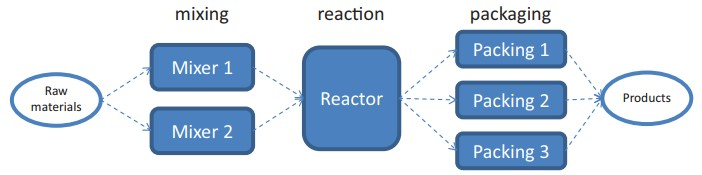
\includegraphics[width=0.8\textwidth]{Bilder/fiktiver_artikel.jpg}
\vspace{0em}
 \caption[]{Fiktiver Prozess des Artikels \cite[S. 3]{ISA-S95_sharing_data}}\label{fig:fiktiver_prozess}
\end{figure}

In der Abbildung \ref{fig:fiktiver_prozess} ist eine Schema einer Prozesskette eines Batchprozess; vom Rohmaterial, bis zum fertigen Produkt; abgebildet. Die verfahrenstechnischen Schritte sind das homogenisieren mittels Mixer (zwei verfügbar), der Reaktor, in dem die chemische Reaktion stattfindet und die Verpackung, wofür drei Packstationen oder Abfüllungen zur Verfügung stehen. In der Abbildung \ref{fig:processsegment_visu} ist das Datenformat der Prozesssegment XSD, in visualisierter Form, dargestellt. Es ist eine hierarchische Struktur zu erkennen. Der Hierarchieursprung wird \textbf{Wurzelelement} genannt und ist in dieser XSD Visualisierung \textit{ProcessSegmentInformation}. Jede B2MML oder BatchML Datei hat einen identischen Aufbau. \textit{ProcessSegmentInformation} ID (1) könnte z.B. \glqq Wirbelschichtrreaktionsprozess\grqq{} heißen. Demnach gäbe es drei \textit{ProcessSegment} ID's (2); für \glqq mixing\grqq, \glqq reaction\grqq, \glqq packaging\grqq. Da sich Equipment des gleichen Typs, z.B. Mixer, in ihrer Funktion unterscheiden können, empfiehlt es sich ggf. \textit{EquipmentClassID's} (3) zu vergeben. Des Weiteren können Abhangigkeiten (\textit{engl. Dependency}) zwischen den \textit{ProcessSegments} existieren, die unter dem Reiter \textit{SegmentDependency} (4 - 6) genau definiert werden können. 

\begin{figure}[h!] %[htbp!] 
\begin{flushleft}
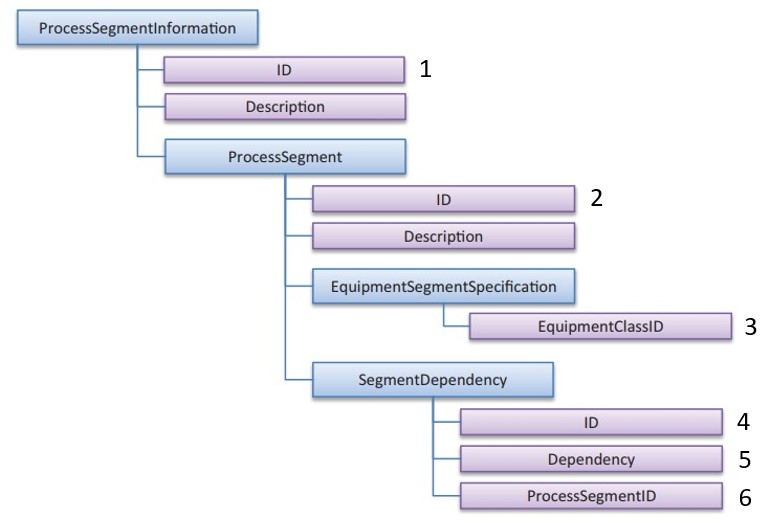
\includegraphics[width=1\textwidth]{Bilder/processsegment_visu.jpg}
\vspace{0em}
 \caption[]{Prozesssegment Informationen \cite{ISA-S95_sharing_data}}\label{fig:processsegment_visu}
\end{flushleft}
\end{figure}
In der folgenden Liste ist ein Teil der vordefinierten, der auf der MESA frei erhältlichen XSD-Files, nach Erstellung eines Accounts, aufgelistet \cite{B2MML}:

\begin{enumerate}[label = \textbullet , itemsep = -0.2em]
\item ProcessSegmentInformation (B2MML-V0600-ProcessSegment.xsd)
\item EquipmentInformation (B2MML-V0600-Equipment.xsd)
\item MaterialInformation (B2MML-V0600-Material.xsd)
\item PersonnelInformation (B2MML-V0600-Personnel.xsd)
\item OperationsCapability (B2MML-V0600-OperationsCapability.xsd)
\item OperationsDefinitionInformation (B2MML-V0600-OperationsDefinition.xsd)
\item OperationsSchedule (B2MML-V0600-OperationsSchedule.xsd)
\item OperationsResponse (B2MML-V0600-OperationsPerformance.xsd)
\item BatchML-V0600-BatchInformation.xsd
\item BatchML-V0600-BatchProductionRecord.xsd
\item BatchML-V0600-GeneralRecipe.xsd
\end{enumerate}
 


\section{Konzeptentwicklung für die Labordigitalisierung}
\label{sec:konzeptentwicklung}

In diesem Abschnitt werden die Konzepte erläutert, die im Verlauf des Projekts erarbeitet werden. Es werden zwei Konzepte entwickelt, die auf das gesamte verfahrenstechnische Labor angewendet werden können. Die Konzepte schließen sich nicht gegenseitig aus, sondern bauen aufeinander auf. Als erstes wird das Konzept erläutert, welches auf die Verwendung einer Datenbank verzichtet. 
Als zweites wird ein Konzept erläutert, in dessen Zentrum sich eine Datenbank befindet. Die Datenübertragungswege sind durchnummeriert. Des Weiteren gibt es pro vorgestelltem Entwurf alternative Datenübertragungswege oder Lösungen die jedoch nicht betrachtet werden. \\

Es wurden \textbf{Anforderungen} für die Konzeptionierung definiert, die nachfolgend aufgelistet sind: 


\begin{enumerate}[leftmargin = 1.2em, label = \textbullet , itemsep = 0.1em]
\item Das Konzept soll für das verfahrenstechnische Labor allgemeingültig sein.
\item Die \glqq digitalen Kompetenzen\grqq{} der Studierenden sollen maximiert werden, ohne die fachlichen Kompetenzen signifikant zu reduzieren, durch 
\item ein Minimum an Automatisierung.

	\begin{enumerate}[leftmargin = 1.2em, label = -- , itemsep = 0.1em]
	\item Unter Automatisierung kann z.B.  die Manipulation von Daten, wie die Detektion von Ausreißer und dessen Entfernung, genaue Leitfäden in der Handhabung, die keine Fehler mehr zulassen o.ä., verstanden werden.
\end{enumerate}
	
\item Der monetäre Aufwand soll minimal sein.
\item Möglichkeiten der Datenerfassung/Signalverarbeitung sollen eruiert werden. 
\item Die inkrementelle Implementation von Applikationen im Rahmen von Industrie 4.0 und Big Data (KI, Digital Twin etc.) soll tendenziell möglich sein.
\item Cloud Computing soll in Betracht gezogen werden.

	\begin{enumerate}[leftmargin = 1.2em, label = -- , itemsep = 0.1em]
	\item Erster Schritt der Umsetzung: Speicherung der Rohdaten auf der HAW Cloud
	\item Zweiter Schritt der Umsetzung: Cloudnutzung, gemäß des Impulsvortrags zum Digitalisierungsfond $\Rightarrow$ Amazon, Google, Microsoft Azure
	\end{enumerate}
	
\item Die gesamte Protokollierung der Studierenden soll in Zukunft digital sein.
\end{enumerate}


\subsection{Konzeptentwurf 3.0 (ohne Datenbank)}

In der Abbildung \ref{digitalisierungskonzept_ohne_db} ist ein Digitalisierungsentwurf ohne die Verwendung einer Datenbank dargestellt. Die Feldebene auf der linken Seite der Abbildung und die Softwareebene sind durch eine \textcolor{orange}{Strich-Doppelpunkt Linie} voneinander getrennt. Der Feldebene sind Feldgerätedaten und Daten, die manuell eingegeben werden müssen, zugeordnet. Die Datenerfassung und das Schreiben von Messwertdaten in CSV-Dateien, die Auswertung und die Protokollierung sind der Softwareebene zugeordnet. CSV-Dateien sind Textdateien, die in ein Tabellenkalkulationsprogramm importiert werden können, deren Spalten durch ein frei wählbares Trennzeichen getrennt sind. In den folgenden sechs Absätzen werden die Elemente der Feld- und Softwareebene erläutert.\\

\bild{1.0}
{digitalisierungskonzept_ohne_db.png}
{0em}
{Digitalisierungsentwurf ohne Datenbank}
{Digitalisierungsentwurf ohne Datenbank}
{digitalisierungskonzept_ohne_db}

\paragraph*{Feldgerätedaten} Die Feldgerätedaten, wie z.B. welche Anlage, Maschine, Messeinrichtung und deren Messwertdaten sind der Feldebene zugeordnet. Auch die Signale oder Daten, die von einem Gerät erfasst werden, sind der Feldgeräteebene zugeordnet.

\paragraph*{Manueller Dateninput} Dem manuellen Dateninput sind alle Daten zugeordnet, die  dokumentiert werden müssen. Unter den zu dokumentierenden Daten können Versuchsparameter wie die Partikeldichte, die Schüttgutmasse etc. sein. Organisatorische Daten sind ebenfalls zu dokumentieren und können bspw. die Gruppen ID, Anwesenheitsinfomationen o.ä. sein.

\paragraph*{Datenerfassung} Für die Datenerfassung, auch Datenakquisition (DAQ~, \textit{engl. data acquisition}) bieten sich Lösungen mit einer grafischen Benutzeroberfläche (\textit{engl. graphic user interface, GUI}) an. Die Datenerfassung kann mittels einer grafischen Programmiersprache wie z.B. LabVIEW realisiert werden oder mit einer textbasierten Programmiersprache wie bspw. Python \cite{low-cost_daq}. Des Weiteren ist eine Datenerfassungssoftware der Gerätehersteller ebenfalls denkbar, (z.B. Laserbeugung-Partikelgrößenanalyse). Datenmanipulationen während der Datenerfassungen müssen dokumentiert und nachvollzogen werden können.

\paragraph*{Messwert-Datalogging} Die diskreten oder kontinuierlichen Daten von Messeinrichtungen können in eine Datei geschrieben werden. Prinzipiell sind zwei Datenformate möglich, das schreiben der Daten im ASCII-Format oder binär. Das entscheidende Auswahlkriterium ist der Speicherbedarf (vgl. Abbildung \ref{fig:speicherbedarf_vergleich} im Anhang  \cite[S. 44]{speicherbedarf_vergleich_binär-ascii}). Eine etablierte Dateiform für Messungsdaten ist die Speicherung in Text-Dateien, genannt CSV-Datei. CSV steht für comma separated value. Die Spalteneinträge sind durch ein Spaltentrennzeichen (engl. \textit{delimiter}) getrennt. Als Spaltentrennzeichen kann neben dem Komma ein beliebiges Zeichen gewählt werden. Die Lösung des Dataloggings in CSV-Dateien hat einen geringen Speicherbedarf (z.B. im vgl. zu Excels *.xlsx-Dateien), da nur \glqq Nutzdaten\grqq{} sowie delimiter, jedoch keine Formatierungsinformation oder der Gleichen vorhanden sind \cite[S. 319]{HandbuchfuerLabview}.

\paragraph*{Auswertung} Die Auswertung kann je nach Vorgabe mit entsprechenden Softwarelösungen (Excel, Matlab, Python etc.) realisiert werden. Die Rohdaten (\textit{engl. raw data}) aus den CSV-Dateien können bspw. in Excel importiert und weiter verarbeitet werden.

\paragraph*{Protokollierung} Das Digitalisierungskonzept welches ohne die Nutzung einer Datenbank auskommt, nutzt zur Datenarchivierung und Protokollierung ein sog. Elektronisches Labor Notebook (ELN), auch Labor Journal genannt. In ELN's können Eingabemasken für diskrete Daten (Versuchsparameter, organisatorische Informationen...) generiert werden. Des Weiteren lassen sich gängige Dateiformate per drag and drop zur Dokumentation in ein ELN importieren \cite[S.44 f.]{ELN_laborjournal}.\\

Die durch die Sensoren erfassten Messwerte werden, z.B. über eine RS-232 Schnittstelle, an die Datenerfassungssoftware übertragen (1). Als Datenerfassungssoftware könnte beispielsweise LabVIEW genutzt werden. Die Versuchssinformationen, Zeitreihendaten und Beobachtung während der Versuche können in der Datenerfassungssoftware aufgenommen werden (2). Die erfassten Daten und ggf. Beobachtungen, werden in eine Textdatei (CSV) geschrieben (3). Im englischen Sprachgebrauch wird ein Punkt als Dezimaltrennzeichen verwendet, woraus die Verwendung des Kommas als delimiter keinem Konflikt gegenübersteht. Im deutschsprachigem Raum ist das Komma jedoch nicht als delimiter zum empfehlen \cite[Vorwort]{HandbuchfuerLabview}. Als delimiter für die Spalten in der Textdatei bietet sich das \texttt{Tabualtor} Zeichen an. Es ist gefordert, dass die generierten CSV-Dateien schreibgeschützt sein sollen. Eine Speicherung der Rohdaten soll auf die HAW Cloud erfolgen. Die Rohdaten der Versuche können für die Auswertung bspw. in Excel importiert (4) und sollen dem Protokoll als Anlage angehängt werden (5). Alle zweckmäßigen Datenmanipulationen, die auf den Pfaden 3 bis 6 durchgeführt werden, müssen bekannt und nachvollziehbar dokumentiert werden. Zweckmäßige Datenmanipulationen könnten Glättungsoperationen der Daten, wie der gleitender Mittelwert, die Entfernung von Ausreißern, das Logarithmieren etc. sein.

\subsection{Konzeptentwurf 4.0 (mit Datenbank und Softwarevernetzungsmöglichkeiten)}

In der Abbildung \ref{digitalisierungskonzept_mit_db} ist eine Erweiterung des zuvor dargestellten Konzepts dargestellt. Im Zentrum dieses Entwurfs steht die Verwendung einer \textcolor{OliveGreen}{Datenbank}. Der Softwareebene wurden bei diesem Konzept drei Elemente hinzugefügt. Nachfolgend werden die drei Elemente erläutert.

\bild{1}
{digitalisierungskonzept_mit_db.png}
{0em}
{Digitalisierungsentwurf mit Datenbank}
{Digitalisierungsentwurf mit Datenbank}
{digitalisierungskonzept_mit_db}



\paragraph*{Datenbank} Es könnte eine lokale oder eine cloudbasierte Datenbank zum Einsatz kommen. Auf dem Mark gibt es Dienstleister, die cloudbasierte Lösungen anbieten. Deren Geschäftsmodelle werden X-as-a-Service gennant. Das X dient als Platzhalter für Plattform, Database, Infrastructure, Software etc. \cite{cloudcomputing_insider}. Die Vorteile und Nachteile von Plattform- oder Database-as-a-Service sind in der Tabelle \ref{xaas} aufgelistet \cite{cloudcomputing, dbmserklaert, cloudcomputing_insider}, werden im Rahmen dieser Arbeit jedoch nicht näher erläutert. 

\begin{table}[t]
\caption{Vor- und Nachteile der Nutzung von Database- oder Plattform-as-a-Service, gemäß der Quellen \cite{cloudcomputing, dbmserklaert, cloudcomputing_insider}} \label{xaas}
\begin{center}
\begin{tabularx}{1\textwidth}{X|X}
Vorteile & Nachteile \\ \toprule
+ \,Kostenersparnis & - \,Abhängigkeit vom Dienstleister\\
\quad \textbullet \,Desaster Recovery Maßnahmen & \quad \textbullet \,Unzureichende Kapazitäten \\
\quad \textbullet \,Updates, Wartung, Instandhaltung & \quad \textbullet \,Insolvenz \\
\quad \textbullet \,Infrastruktur 									& \quad \textbullet \,Kundenservice \\
\quad \textbullet \,Software 										&  - \,Datenschutz \\
\quad \textbullet \,Personalkosten 	& \quad \textbullet \,Servicestandort oft nicht in EU/Dt.  \\
+ \,Infrastuktur 												& - \,Datensicherheit (Datenverlust) \\
\quad \textbullet \,Rechenleistung								& - \,eigene IT-Kompetenz \\
\quad \textbullet \,Speichekapazität							& - \,Infrastuktur \\
\quad \textbullet \,Netzwerkkapazität 						& \quad \textbullet \,Latenzzeiten \\
+ \,Anpassbar- und Skalierbarkeit 				& \quad \textbullet  \,lokale Ausfälle \\
+ \,Gut kalkulierbare Fixkosten 					& \quad \textbullet  \,lokale Strom- oder Netzwerk Ausfälle\\
+ \,Sicherheit in Bezug.. 								& \\
\quad \textbullet \,auf Mitarbeiter 								& \\
\quad \textbullet \,Dezentralität  & \\
\quad \enspace $\cdot$  Schutz vor lokale Hackerangriffe & \\
\quad \enspace $\cdot$  social hacking Prävention & \\
+ \, Portfoliosoftware Kompatibilität & \\
\end{tabularx}
\end{center}
\end{table}

\paragraph*{Digital Twin} Es existieren verschiedene Formen des sog. \glqq digitalen Zwillings\grqq{} (\textit{engl. Digital Twins}). Mittels \textit{Digital Twins} können Produkte, Produktionsabläufe oder ein gesamter Prozess, durch die Kopplung von Produktions- und Produkt Twin, abgebildet und somit optimiert werden. Mittels Digital Twins lassen sich sogenannte Soft-Sensoren integrieren (angewandte numerische Simulation). In Produktionsprozessabschnitten, in denen die Bedingungen es nicht erlauben einen realen Langzeitsensor zu implementieren, können, mittels Digital Twins, Sensoren in Simulationssoftware generiert werden, die mit einem Prozess synchronisiert sind, um Totzeiten zu verringern oder zu eliminieren, bis schlechte Produktionsbedingungen detektiert werden können. Dadurch kann die Effizienz eines Prozesses signifikant gesteigert werden kann. Für die Simulation mittels Digital Twins werden Prozess-, Rohstoff- und geometrische Daten benötigt. Die Form der Randbedingungen können vielfältig sein und unterscheiden sich je nach Simulationsobjekt. Randbedingungen könnten Parameter der Umgebung betreffend, materialabhängige Parameter oder Parameter, die der Wertschöpfungskette zugehörig sind, sein. Als Beispiel für Parameter der Wertschöpfungskette kann ein tendenziell auftretender Rohstoffengpass durch Lieferverzug seitens des Zulieferers genannt werden \cite{digitwin_prozessmodellierung}. Weitere Informationen ist weiterführenden Fachliteratur zu entnehmen. \\


\paragraph*{Künstliche Intelligenz} Ein Teilgebiet der Informatik ist das Themengebiet der \glqq künstlichen Intelligenz\grqq{} (KI, \textit{engl. artificial intelligence, AI}). Teilgebiete der Künstlichen Intelligenz sind das \textit{Machine Learning} (ergänzung im Anhang), \textit{Robotik}, sog. \textit{Expertensysteme}, Mustererkennung, die Verarbeitung natürlicher Sprache oder maschinelles Übersetzen (deepl.com) \cite{infos_teilgebiete_ai}. 

Die potenziellen Fähigkeiten von KI Applikationen sind das Lernen, Planen und Problemlösen. Die Ansätze sind jedoch humanzetriert, zur Unterstützung der Menschen, bei ihren Tätigkeiten. Präzisiert bedeutet das \cite[S. 5]{techszenario_i40}:

\begin{center}
\begin{tabularx}{1\textwidth}{p{0,45\textwidth}|X}
\hspace{0,5em} \textbullet \,Wissenserwerb & \hspace{0,5em} \textbullet \,kognitives Erfassen und Automatisieren\\
& \hspace{1em} logischer Schlussfolgerungen\\[4pt]
\hspace{0,5em} \textbullet \,Maschinenlernen & \hspace{0,5em} \textbullet \,Planung und Ausführung industrieller \\
& \hspace{1em} Automatisierungsprozesse \\[4pt]
\hspace{0,5em} \textbullet \,Bild- und Spracherkennung &\hspace{0,5em} \textbullet \,Mustererkennung \\
\end{tabularx}
\end{center}




%Einige Algorithmen müssen angelernt werden (\textit{engl. \textbf{supervised} or \textbf{semi-supervised}}), z.B. das vom Google-Brain-Team entwickelte open-source Modell, Tensor Flow \cite{tensorflow_framework}. Andere werden nicht angelernt und generieren Ihren Algorithmus autonom (\textit{engl. \textbf{unsupervised}}; vgl. \ref{fig:supervised_machinelearning} im Anhang). \textbf{Supervised Learning}  (vgl. Abbildung \ref{fig:supervised_machinelearning} im Anhang) bedeutet, dass Datensätze vorgegeben werden und zugleich deren Lösung bzw. Klassifizierungen. Anhand des dadurch generierten Algorithmus werden unbekannte Datensätze klassifiziert. Je nach verwendetem Algorithmus können Klassifizierungen binär wie Spam, nicht Spam; Mann, Frau oder Multi-Class-Klassifizierungen, wie z.B. Porsche, Mercedes, VW, .... sein. \textbf{Semi-Supervised Learning} Algorithmen verändern ihren angelernt Algorithmen, bzw. können Ihren Algorithmus, anhand der unvalidierten Daten, die sie nach dem anlernen erhalten, optimieren. KI Algorithmen benötigen große, Datenmengen. Einfache KI's benötigen zusätzlich strukturierte Daten, damit ist die Verfügbarkeit der Daten in Datenbanken gemeint. Die neusten, komplexen \cite{unstrukturierte_daten_ki} maschine learning Algorithmen können auch mit unstrukturierten Daten verwertbare Ergebnisse generieren, doch es gilt stets GIGO, \glqq garbage in, garbage out!\grqq{} Die Güte der Ergebnisse einer KI wird durch die Güte der Ausgangsdaten bestimmt, demnach ist die Wahrscheinlichkeit mit strukturierten Daten ein sinnvolles, aussagekräftiges Ergebnis zu erzielen wahrscheinlich höher.
%Es existiert noch eine vierte Kategorie, die \textbf{Reinforced Learning} Algorithmen. Diese Algorithmen unterscheiden sich von den unsupervised Algorithmen in der Art, dass sie mit einer Umgebung (\textit{engl. environment}) interagieren und dadurch lernen \cite[S. 15 f.]{machine_learning_kompakt}. Als Beispiele können Roboter oder KI in einem Spiel wie Schach, Go (die asiatische, komplexere Schachvariante), aber auch in Videospielen genannt werden \cite{reinforced_learning_go}.
%
%Zu den \textbf{Unsupervised Lerning} Algorithmen zählen z.B. die Regressionsanalyse oder die k-mean Clusteranalyse \cite[S. 114]{machine_learning_kompakt}. Um bei \textbf{supervised} oder \textbf{semi-supervised} verwertbare Ergebnisse zu erhalten, wird in vielen Anwendungsfällen eine \glqq große\grqq{} Datenbasis benötigt. Des Weiteren ist die Güte der Daten entscheidend für die Güte der Ergebnisse. Weniger komplexe KI Algorithmen benötigen strukturierte Daten, wofür sich Datenbankmanagementsysteme (DBMS) auszeichnen.\\

Der Entwurf aus dem vorherigen Abschnitt wird um die Verwendung einer Datenbank erweitert. Dadurch wird die Nutzung neuer Software  für die Erschließung neuer Prozesse, Prozessoptimierung und/oder Validierung ermöglicht. Die Feldgerätedaten werden, wie bei dem vorherigen Konzept, an eine Datenerfassungsoftware übertragen (\texttt{1}). Die diskreten und/oder kontinuierlichen Daten werden durch die Datenerfassungssoftware direkt in eine Datenbank geschrieben (\texttt{9}). Nach der Einrichtung einer Datenbank ist es theoretisch möglich auf das \textcolor{blue!50}{Messwert-Datalogging} in Form von CSV-Dateien zu verzichten (\texttt{3}), jedoch könnte eine redundante Datensicherung sinnhaft sein. Durch die Verwendung einer Datenbank ergeben sich neue Datenübertragungswege (\texttt{7} - \texttt{11}). Eine Software Schnittstelle wird API (application programming interface) genannt. Sollte, auf Basis dieser Arbeit, eine Machbarkeitsstudie dieses Konzepts erfolgen, dann ist die API Kompatibilität jeglicher potenziell erwünschter Software zu prüfen. Durch die Verwendung einer Datenbank ist es möglich Daten strukturiert zu archivieren (\texttt{7} - \texttt{11}) und mittels sog. Abfragen (\textit{Querys}) mit geringem Aufwand wieder abzurufen (\texttt{7}, \texttt{10}, \texttt{11}). Durch die Verwendung einer Datenbank kann die Nutzung von \glqq einfachen\grqq{} KI's (\texttt{10}) und Digital Twins ermöglicht (\texttt{11}) sowie die Ergebnisse der Berechnungen in der Auswertung diskutiert werden (\texttt{7}).\\

Dem Professor für Umformtechnik sowie stellvertretenden Leiter des Maschinenbau und Produktionstechnik Departments Dr. E. Stöver, bei einem zweistündigem offenem Dialog mit Prof. Dr. C Frank, Prof. Dr. K. Freudenthal, Prof. Dr. Geweke,  Dipl.-Ing. M. Hannappel, Prof. E. Stöver, Dipl.-Ing. S. Wittkowski nach einem Vortrag von mir, D. Ludwig, Beginn \texttt{9} Uhr, zum Ziel der digitalen Transformation des verfahrenstechnischem Labors, mit dem Schwerpunkt dieser Masterthesis, am \texttt{26.08.2020}, von \texttt{9} bis \texttt{12} Uhr, entnehmen, dass die Vision des Konzepts dieser Masterthesis \glqq in die richtige Richtung zeigt\grqq{}. Prof. Dr. Enno Stöver ist dabei, die Idee des \glqq Lernorts Digitale Umformtechnik\grqq{} umzusetzen. Dabei verfolgt er auch die Vision, dass Unternehmen und Studierende in eine Kooperation am Ort der Hochschule kommen. Dabei muss der Professor nicht der Initiator sein, sondern vielmehr der Ort als Treffpunkt die Kooperation auf niedrigem Level begünstigen. Die Vision von Prof. Dr. E. Stöver ist es, den \glqq digitalen Lernort Umformtechnik\grqq{} an der HAW, am Berliner Tor zu etablieren. Lean Runden der Studierenden sind gelebter Alltag und die Vision ist folgende, \label{sec:digitalerlernraum}

\begin{displayquote}
\glqq Der „Lernort Digitale Umformtechnik“ stellt einen physischen Raum und eine virtuelle Plattform für die Lehrenden und die Studierenden der HAW Hamburg, sowie Unternehmen der Metropolregion Hamburg zum Themenbereich Industrie 4.0 und Digitalisierung im Bereich der Umformtechnik dar. Anwendungsbezogene Lösungen werden hier ausprobiert und stehen zum gemeinsamen kompetenzorientierten, forschungsbasierten und digital unterstütztem Lernen bereit. Neue Lösungen werden gemeinsam im Zusammenspiel von Praxis und Lehre entwickelt \cite{digitale_umformtechnik}.\grqq{}
\end{displayquote}

Bei einer Begehung der mechanischen verfahrenstechnischen Einrichtung der TUHH mit Dr. S. Pietsch, am \texttt{14.09.2020}, ab \texttt{14} Uhr, hat sich herausgestellt, dass ein ganzheitliches Konzept, unter der Verwendung einer Datenbank, \textbf{im akademischen Rahmen} \glqq innovativ sein könnte\grqq{}. Die TUHH hat ein Digital Twin Konzept im Projektbacklog, welches innerhalb eines Zeitrahmens von ca. zwei Jahren umgesetzt, bzw. integriert werden soll. Die Implementation eines Datenbankmanagementsystems ist nicht angedacht. Eine Kooperation, mit gegenseitigem Nutzen, könnte möglich sein.\\

Im Verlauf einer ZOOM Präsentation meinerseits, am \texttt{26.10.2020} von \texttt{16:15} Uhr bis \texttt{17:45} Uhr, mit den Teilnehmern Prof. Dr. Geweke, Prof. Dr. Hölling, Prof. Dr. Sievers konnte ich von Prof. Sievers entnehmen, dass ein Vorteil des datenbankorientierten Konzepts, die vereinfachte  Investigationsmöglichkeit bei vermeintlich konstanten Betriebsparametern, jedoch unterschiedlichen Ergebnissen, ist. Daraus ließen sich schneller studentische Projekte ableiten.
Dem Professor der mech. Verfahrenstechnik M. Geweke, konnte ich im Verlauf dieses Meetings entnehmen, dass die Nutzung eines Datenbank orientierten Konzepts einen weiteren Nutzen hat. Die Covid-19 Situation hat Schwächen im konventionellen System aufgezeigt. Eine unstrukturierte, multimediale Archivierung hat einen großen Aufwand erzeugt, um alternative Lehrinhalte zum nicht durchführbarem Verfahrenstechnik sowie Lebensmitteltechnikpraktikum zu generieren.\\

S. Schwemm, B. Sc. Student der Verfahrenstechnik, hat mir in einem kurzem Interview seine Schwierigkeit mit dem daraus resultierenden, \glqq alternativem Lehrinhalt\grqq{} nahegelegt. Die Hypothese die man daraus schlussfolgern könnte ist die folgende, 

\begin{displayquote}
\glqq Die Energie der Professoren, die in die Suche von geeigneten, aufeinander abgestimmten Daten dissipiert ist, hätte und kann in Zukunft vermieden werden. Die somit verfügbare Energie der Professoren, kann zum Optimieren der Lehrinhalte genutzt werden. Zu vermuten, dass der Worst Case eingetroffen und überstanden ist sowie ähnliche Situationen \glqq unwahrscheinlich\grqq{} sind, wäre fahrlässig \grqq.
\end{displayquote}



%Des Weiteren konnte ich dem Prof. für Umformtechnik sowie stellvertretenden Leiter des Maschinenbau und Produktionstechnik Departments Dr. E. Stöver und zugleich erst Betreuer dieses Projekts entnehmen, dass die Vision dieses Konzepts \glqq in die richtige Richtung zeigt\grqq{}. Prof. Dr. E. Stöver ist dabei die Vision eines digitalen Lehrnorts an der HAW am Berliner Tor zu etablieren. Lean Runden der Studierenden sind gelebter Alltag und die Vision ist folgende, \label{sec:digitalerlernraum}





%\begin{displayquote}
%\glqq Studierende arbeiten autonom an Projekt mit Unternehmen aus den verschiedensten Branchen, wie z.B. der Luftfahrt, Automobilindustrie, Werkzeugbau uvm.. Prof. E. Stöver betritt den Lehrnraum am Berliner Tor, \glqq hat keine Ahnung\grqq{} woran Studierende mit Ingenieuren aus den Unternehmen arbeiten. Zwischen den Zeilen steht ein Paradigmenwechsel. Die flachen Hierarchien die bereits in modernen oder novellierten Unternehmen gelebt wird erhält Einzug im Studium. Unternehmen werden die Lehre Formen und nicht Professoren die \glqq 50 Jahre\grqq{} nicht mehr in der Industrie tätig waren. \grqq{}
%\end{displayquote}

\subsection{Fazit}

Das verfahrenstechnische Labor soll, zeitgemäß, digital transformiert werden. An der Stelle muss nochmals erwähnt werden, dass eine digitale Transformation ein Prozess und kein Projekt ist. Die beiden vorgestellten Konzepte schließen sich nicht gegenseitig aus. Das Konzept ohne Datenbank (DB) kann als Vorstufe des Konzept mit einer DB betrachtet werden. Das Konzept 3.0 ist eine Mindestanforderung für die digitale Transformation des verfahrenstechnischem Labors. Ein Ziel dieses Projekts ist es, Messwerte digital verfügbar zu machen und diese zu dokumentieren. Ein weiteres Ziel des Projekts ist es einen Wandel von der Versuchsdokumentation in Hardcopy, zu einer digitalen Dokumentation einzuleiten. Es ist anzumerken, dass dieses Konzept die \textbf{\emph{\underline{absolute Mindestanforderung}}} für den ersten Schritt in die digitale Transformation darstellt.\\

Im folgenden werden die Vorteile des Konzepts ohne eine Datenbank aufgelistet: 

\begin{itemize}
\singlespacing
\item Die Verfügbarkeit von digitalen Messwerten wird ermöglicht, 
\item Die Dokumentation der Versuchsrandbedingung, eingesetzte Rohstoffe etc. kann digital durchgeführt werden,
\item Die Verfügbarkeit der Versuchsdaten und Ergebnisse wird durch die Einführung eines elektronischen Labor Notebooks verbessert,
\item Versuchsbeobachtungen können direkt dem Zeitstempel zugeordnet werden.
\end{itemize}



%An dieser Stelle nun ein radikales dennoch wahres Beispiel aus meinem sechsten und siebten, Semester des erst Studiums, im Jahr 2017.
%
%\glqq Ich persönlich habe Vorlesungen, \textbf{\emph{\underline{mit Potential}}}, besuchen müssen, in denen \textbf{permanent} teilweise unlesbare Zeitungsartikel aus dem Jahr 19XX auf \textit{Over Head Projektoren} abgebildet wurden.\grqq{} Wie war das noch mit dem Stand der Technik? Das ist ebenfalls eine bis dato gelebte Mindestanforderung an der Hochschule! Eine harte, traurige, dennoch ware Tatsache!

Eine Mindestanforderung sollte jedoch kein Maßstab für eine Hochschule darstellen! Meines Erachtens nach unterliegt der Aufwand dem Nutzen der Konzeptrealisierung unter der Verwendung einer Datenbank im hohem Maße, aus den folgenden Gründen. 

Im akademischen Rahmen unterliegt der Aufwand, der Realisierung des zweiten Konzepts mit Datenbank, einen \textbf{großen} Mehrwert in Bezug auf das Verständnis und Lernerfolg der Studierenden. Die Datenbank könnte auch für den Laborbetrieb des Departments genutzt werden, wodurch sich möglicherweise organisatorische Vereinfachungen, wie z.B. Chemie- und Verfahrenstechniklagerverwaltung o.ä. realisieren lassen. Des Weiteren könnte die Datenbank für die verfahrenstechnische Forschung, Projekte im Rahmen der angewandten numerische Simulation uvm. genutzt werden.. Die \textbf{größte Hürde} für die Konzept 4.0 Realisierung könnte der \textbf{Changeprozess} sein.\\

In unserer agitierten Welt ist weder Platz für schwere Unternehmenstanker noch für träge Universitäten oder Hochschulen. In der Zeit der Globalisierung und digitalen Transformation ist Flexibilität und Vernetzung nicht nur eine hinreichende Forderung, sondern absolut notwendig. Unternehmen sollten sich Ihre Spitzenkräfte schaffen. Der Spruch, \glqq von der Berufsausbildung oder dem Studium braucht man am Ende des Tages maximal 15 \%\grqq , ist nicht tolerierbar sowie zu verantworten und doch ist es aus eigenen Erfahrungen Realität. Wie lange Überlebt ein Unternehmen welches 85 \% Ausschuss hat? Wenn durch diese Art des Paradigmenwechsels eine Ausschussreduktion auf bspw. 70 \% erfolgt, ist das ein immenser Fortschritt! 
In der Tabelle \ref{tab:konzept4.0} sind die Vor- und Nachteile des Konzepts 4.0 aufgelistet.

%\begin{table}[t]
%\caption{Vor- und Nachteile der Nutzung von Database- oder Plattform-as-a-Service \cite{cloudcomputing, dbmserklaert, cloudcomputing_insider}} \label{xaas}
%\begin{center}
%\begin{tabularx}{1\textwidth}{X|X}
%Vorteile & Nachteile \\ \toprule
%+ \,Stand der Technik in der Industrie	/ Zeitgemäß			& - \,notwendiges Know-How erforderlich \\
%+ \,Nutzbar für Tätigkeiten außerhalb vom VT1 und VT2 Praktikum	& -  \,Aufwand der Erstellung der Datenbank \\
%+ \,wenn Cloudservicenutzung, dann Port\-folio\-software Kompatibilität des Anbieters & - \,Einrichtung automatischer Einspeisung der Sensordaten in die Datenbank \\
%+ \,Image/Professionalität (u.a. auch Anmerkungen von Bachelorranten) & \\
%+ \,vllt. mehr Kooperationsprojekte mit Unternehmen und Universitäten & \\  
%+ \,Kompetenzsteigerung der Hochschule und Absolventen & \\
%+ \,interdisziplinäre Vernetzung/Projekte  (Industrie 4.0 $\equiv$ Vernetzung) &\\
%
%\end{tabularx}
%\end{center}
%\end{table}


%\begin{table}[t]
%\caption{Vor- und Nachteile der Nutzung von Database- oder Plattform-as-a-Service \cite{cloudcomputing, dbmserklaert, cloudcomputing_insider}} \label{xaas}
%\begin{center}
%\begin{tabular}{L{0,3em}L{16em}|L{0,3em}L{16em}}
%&Vorteile & &Nachteile \\ \toprule
%+ & Stand der Technik in der Industrie	/ Zeitgemäß			&-\,- & Changeprozesse \\
%+ & Nutzbar für Tätigkeiten außerhalb vom VT1 und VT2 Praktikum (Forschung, Organisatorisches wie Lagerverwaltung, angewandte numerische Simulation	uvm.) & -  &notwendiges Know-How erforderlich \\
%+ & wenn Cloudservicenutzung, dann Port\-folio\-software Kompatibilität des \mbox{Anbieters} & -  & Aufwand der Erstellung der Datenbank \\
%+ & Image/Professionalität (u.a. auch Anmerkungen von Bachelorranten) & - & Einrichtung automatischer Einspeisung der Sensordaten in die Datenbank\\
%+ & vllt. mehr Kooperationsprojekte mit Unternehmen und Universitäten & - & Kosten könnten entstehen\\  
%+ & Kompetenzsteigerung der Hochschule und Absolventen & \enspace \textbullet & Sponsoring da Hochschule (oder vllt. als Gegenleistung Projekte o.ä)\\
%+ & interdisziplinäre Vernetzung/Projekte  (Industrie 4.0 $\equiv$ Vernetzung) & \enspace \textbullet & geringe Datenmengen im vgl. zu Unternehmen \\
%+ & gute Investigationsmöglichkeiten bei Produktabweichung bei konstanten Parametern $\rightarrow$ Studentenprojekten & \enspace \textbullet & Wissenschaftlichermitarbeiter für die digitale Transformation \\
%\end{tabular}
%\end{center}
%\end{table}

\begin{table}[h!]
\caption{Vor- und Nachteile des Konzeptentwurfs 4.0} \label{tab:konzept4.0}
\begin{center}
\begin{tabularx}{1\textwidth}{X|X}
Vorteile & Nachteile \\ \toprule \vspace{-1,5em}
\begin{itemize}[leftmargin=*,labelsep=-\mylen]
\item[+] Stand der Technik in der Industrie	/ Zeitgemäß 
\item[+] Nutzbar für Tätigkeiten außerhalb vom VT1 und VT2 Praktikum (Forschung, Organisatorisches 
wie 
\item[+] Lagerverwaltung, angewandte numerische Simulation	uvm.)
\item[+] wenn Cloudservicenutzung, dann Port\-folio\-software Kompatibilität des \mbox{Anbieters}
\item[+] Image/Professionalität (u.a. auch Anmerkungen von Bachelorabsolventen Ende 2020)
\item[+] ggf. mehr Kooperationsprojekte mit Unternehmen und Universitäten
\item[+] Kompetenzsteigerung der Hochschule und Absolventen
\item[+] interdisziplinäre Vernetzung/Projekte  (Industrie 4.0 $\equiv$ Vernetzung)
\item[+] gute Investigationsmöglichkeiten bei Produktabweichung bei konstanten Parametern $\rightarrow$ Studentenprojekte
\end{itemize}

&
\vspace{-1,5em}
\begin{itemize}[leftmargin=*,labelsep=-\mylen]
\item[--] Changeprozesse
\item[-] notwendiges Know-How erforderlich
\item[-] Aufwand der Erstellung der Datenbank
\item[-] Einrichtung automatischer Einspeisung der Sensordaten in die Datenbank
\item[-] Kosten könnten entstehen
\begin{itemize}[leftmargin=*,labelsep=-\mylen] 
\item[\textbullet] möglicherweise Sponsoring/Kooperation (als Gegenleistung Projekte o.ä) da Hochschule 
\item[\textbullet] geringe Datenmengen im vgl. zu Unternehmen $\rightarrow$ möglicherweise keine oder geringe Kosten
\end{itemize}

\end{itemize}
\end{tabularx}
\end{center}
\end{table}

\pagebreak

%\subsubsection{Das Attentat}
%
%Ich habe während des Masters ein Lösungskonzept für das Unternehmen entworfen, bei dem ich meine Berufsausbildung absolviert habe. Ziel des Konzept ist eine bessere Qualitätskontrolle, Ausschussminimierung durch schenlle Datenkorrelation (Vereinfachung der Korrelation von Ausschuss und Produktionsparametern; es ist nicht trivial, weil lange Totzeiten vorhanden und nicht alle Prozessdaten verfügbar und einige Prozessschritte nicht automatisiert sind…Industrie 2.5 bzw. dritter Kondratjew-Zyklus lässt grüßen haha) Dieses Besteht im Kern aus der Anwendung einer Maschine Learning Lösung. Das notwendige Wissen dazu habe ich noch nicht, traue mir jedoch zu es mir aneignen zu können. \\
%
%In meinem Ausbildungsbetrieb würde ich \textbf{sehr} gut verdienen (als Facharbeiter habe ich bereits 2700 € Netto verdient; IG Chemie), doch es könnte ein Dead End, zuzüglich Unzufriedenheit sein und Geld ist bei weitem nicht alles. Es sind sehr steile Hierarchien in meinem alten Unternehmen, zudem haben die potentiellen, alt eingesessenen Vorgesetzten nicht die Kompetenzen, die man sich von vorgesetzten wünscht oder ein Visionäres Mindset, welches den Mangel an wünschenswerten Kompetenzen kompensieren würde. Der Job wäre nur ein Zwischenstopp und eine Zwangsmaßnahme, um meine ethischen Pflichten zu erfüllen (unten wird’s klar) und endlich mal paar Euros zu verdienen. Es gibt noch weitere Unternehmen in meinem Anschreiben Portfolio, doch…\\
% 
%Ich habe vor zu promovieren und möglicherweise könnte das Projekt der digitalen Transformation der Verfahrenstechnik an der HAW als Promotionsthema dienen. Wir alle könnten synergetisch von meiner Vision profitieren. Ich traue mir zu das Projekt, "digitale Transformation", zu der Zufriedenheit "aller (Changeprozesse lassen grüßen)" voranzutreiben, aufbauend auf dem Konzept welches Sie gelesen haben. Die sich daraus resultierenden Changeprozesse würde ich selbsterklärend auch übernehmen. Sie wissen ja bereits was für einen, ich nenne es mal, Exzentriker Sie sich ins Boot holen würden. Ich bin ein sehr guter Selbstmotivator und in Folge dessen bin ich eine Selbstständig arbeitende Persönlichkeit, was man definitiv für solch ein Projekt braucht. \\
% 
%Nietzsche sagte einst: „Wer ein Warum hat, kann fast jedes wie ertragen.“ \\
% 
%Das ist einer meiner zentralen Glaubenssätze, der mein inhärentes Wertesystem dominiert und dass von klein auf, bevor ich wusste dass es Nitzsche mal gegeben hat. Ich strebe stets nach Verbesserungen, in jeglichem Aspekt in meinem Leben und habe Lust irgendwas in digitaler Richtung zu machen. Für meine Visionären Ziele muss ich mir Kompetenzen der aufstrebenden Branche des Data Scientist, das Data Mining, Maschine Learning etc. aneignen (mein Warum), auch wenn es ein viel Arbeit und Anstrengung bedeutet (Wie). Teile dieser Kompetenzen könnte ich mir im Rahmen des Projekts synergetisch aneignen.\\
% 
%Ich habe selbstverständlich auch noch weitere private Anreize. Ich leben mit meiner kranken Mutter (66 jahre, 13\% Herzleistung ist nur die Spitze des Eisbergs) zusammen und kümmere mich nebenher auch noch um meinen unsympathischen Stiefvater (82 Jahre), der ebenfalls in Bergedorf wohnt. In diesem Sinne würde ich die Möglichkeit bekommen meinen Doktortitel, sofern dieses Projekt dazu geeignet ist, zu machen, meine moralischen/ethischen Pflichten zu erfüllen und Sie hätten jemanden mit hinreichender Qualifikation, der sich diesem Projekt annehmen würde. Ich könnte mit dem stellv. Departementsleiter für Maschinenbau und Produktionstechnik Prof. Enno Stöver vernetzt bleiben, da ich seine Hochschulvision als einzig wahre Lösung ansehe. Da Die TUHH nun bald mit dem Projekt des Digital Twins startet, wäre es vllt. möglich einen Doktorvater von dort zu organisieren, wodurch möglicherweise eine tiefgreifendere Kooperation zwischen der TUHH und HAW zu Stande kommt. \\
%
%Sie, Stefan und Marc hingegen könne sich noch mehr auf Ihre Berufung, dass Schmieden von Studenten, fokussieren.\\
% 
%Des Weiteren bietet mir dieses Projekt die Möglichkeit meine gewünschten Kompetenzen \textbf{synergetisch mit/zum guten Zweck, der Verbesserung der Lehre}, anzueignen. An dieser Stelle nun eine radikale dennoch wahre Anekdote aus meinem sechsten und siebten, Semester des erst Studiums, im Jahr 2017 (Ursprünglich war \textcolor{black!70}{der folgende Absatz} in der Thesis, doch viele kommen mit meiner, zugegeben, oftmals undiplomatischen Ehrlichkeit nicht zurecht, daher ist er nun hier..).\\
%
%\textcolor{black!70}{"Ich persönlich habe Vorlesungen, \textbf{mit Potential}, besuchen müssen, in denen permanent teilweise unlesbare Zeitungsartikel aus dem Jahr 19XX auf Over Head Projektoren abgebildet wurden." Wie war das noch mit dem Stand der Technik? Das ist ebenfalls eine bis dato gelebte Mindestanforderung an der Hochschule! Eine harte, traurige, dennoch wahre Tatsache!
%Durch die nicht hinreichende Mindestanforderung habe ich die Vorlesungen im Grunde nicht verstanden.}\\
%
%Durch die Arbeit an der HAW hätte ich zu diesen "besonderen" Zeiten möglicherweise weniger Menschenkontakt als in einem Betrieb und kann dadurch ein potentielles gesundheitliches/sterbe Risiko für meine geliebten Mitmenschen reduzieren, denn um mich mache ich mir in Bezug auf Covid keine sorgen (Sport, gesunde Ernährung, kaltes Abduschen etc.). Bei wieviel Wins sind wir nun?\\
% 
%Wie bin ich nun auf die ganze Kiste gekommen, haha. simultan zum Schreiben des Absatzes „Konzeptentwurf 4.0 (mit Datenbank)“, denn der Lösungsansatz für meinen Ausbildungsbetrieb hat seit dem ersten Mastersemester meine berufliche Vision dominiert. Nun, können Sie darüber kontemplieren und sich ggf. beraten, ob Sie diesen lateral denkenden „Chaoten“ ins Boot holen wollen.\\
% 
%Mit allerbesten Grüßen\\
% 
%Daniel Ludwig\\
%
%PS Bisschen Spaß muss sein, wie man dem Schriftstück entnehmen kann, sonst wird die Welt noch grauer als sie von Natur aus sein kann :)
%%\subsection{Datenstrukturentwurf einer relationalen Datenbank}

\subsection{Strukturkonzept einer relationalen Datenbank}

Im Rahmen dieser Projektarbeit wurde eine Datenstruktur für eine relationale Datenbank entworfen. Das Konzept wurde der\textit{ ISA-S95} Struktur nachempfunden. ISA-S95 gliedert Unternehmen hierarchisch auf. Eine Datenstruktur gibt ISA-S95 jedoch nicht vor. \textit{Abteilungen} und \textit{Rubriken} werden demnach hierarchisch aufgegliedert. Eine Rubrik könnte bspw. alle Informationen ({\Hypatia 100\_Informations}) sein, dazu später mehr. Die Unterteilung erfolgt demnach von einem \textit{Wurzelelement} (\textit{engl. rootelement}) in \textit{Abzweigungen} (\textit{engl. branchelements}) und \textit{Dokumentreferenzen} (\textit{engl. sheetelements}; siehe Abbildung \ref{fig:root_branch}). An der Bezeichnung \textit{Dokumentreferenzen} lässt sich erkennen, dass die strukturvorgabe Dokumentenbasiert erfolgt. Eine präzisierung erfolgt an anderer Stelle.

\begin{figure}[h!] %[htbp!] 
\centering
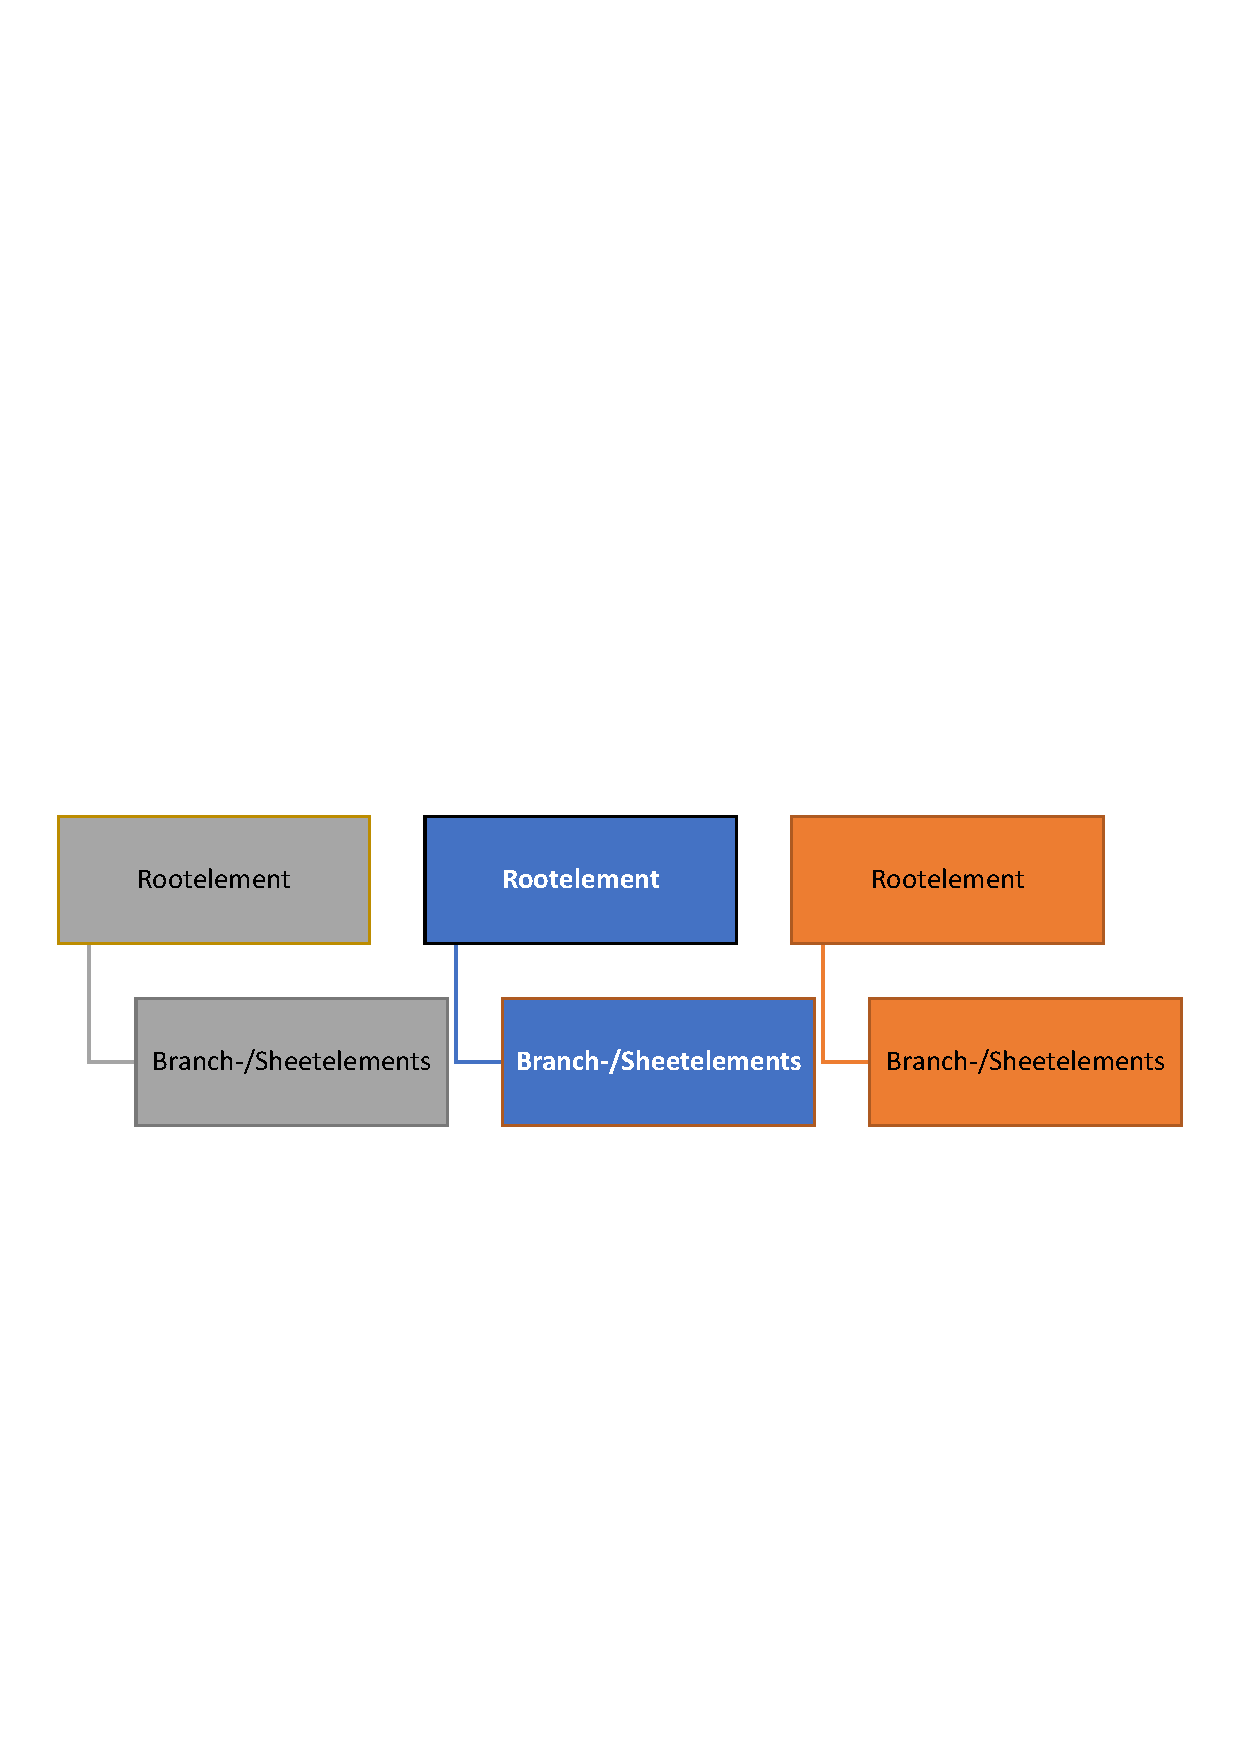
\includegraphics[width=0.8\textwidth]{Bilder/DB/Root_Branchelements.pdf}
\vspace{0em}
 \caption[Root-/Branchelements, gemäß ISA-S95]{Root-/Branchelements, gemäß ISA-S95}\label{fig:root_branch}
\end{figure}

\paragraph*{Anmerkung:} Die Grafiken dieses Abschnitts und denen im Anhang erheben keinen Anspruch auf \newline Vollständigkeit und Konsistenz. Die Erstellung der Grafiken wurden manuell in PowerPoint und keinem professionellem Tool erstellt, Tabellen und  Bezeichnungen haben demnach keine Referenzfunktion. Zur Darlegung der konzeptionellen Idee sollte die Güte der Qualität hinreichend sein.

Für die Verfahrenstechnik wurde im Rahmen dieses Projekts eine hierarchische Gliederung durchgeführt (siehe Abbildung \ref{fig:hierarchisch_vt}). Es wurden drei \textit{rootelements} definiert. Die unterschiedlichen Farben dienen im Verlauf dieses Abschnitts der visuellen Differenzierung der \textit{Rubriken}. 



\begin{figure}[h!] %[htbp!] 
\centering
%\vspace{-4em}
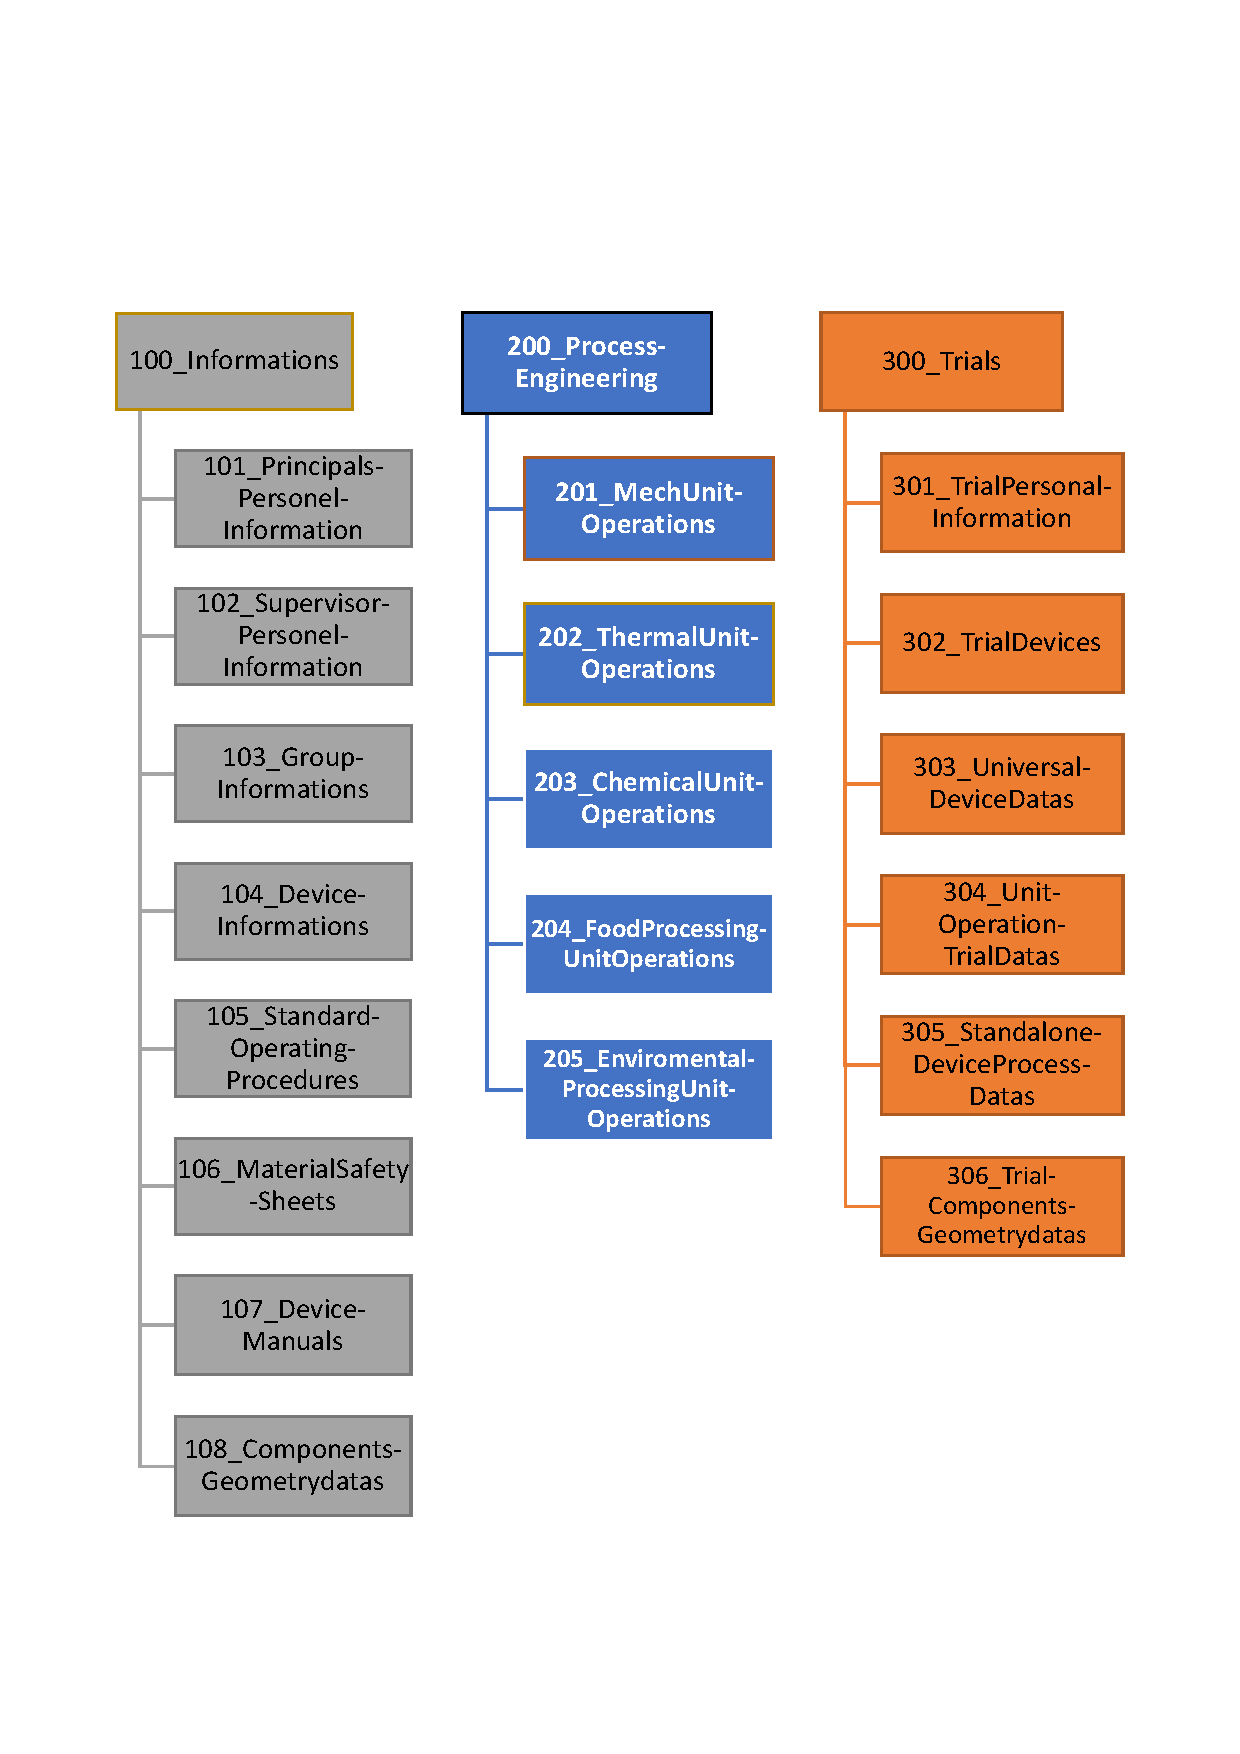
\includegraphics[width=.8\textwidth]{Bilder/DB/Labordatenstrukturdarstellung_im_ISA-95 Standard.pdf}
%\vspace{-4em}
 \caption[Labordatenstrukturdarstellung, angelehnt an ISA-S95]
 {Labordatenstrukturdarstellung, angelehnt an ISA-S95}\label{fig:hierarchisch_vt}
\end{figure}

\begin{itemize}
\item \textcolor{black!50}{{\Hypatia 100\_Informations}}
\item \textcolor{blue!90}{{\Hypatia 200\_ProcessEngineering}}
\item \textcolor{orange}{{\Hypatia 300\_Trials}}
\end{itemize}

Dem \textit{rootelement} {\Hypatia 100\_Informations} sind alle \textit{branch-} und \textit{sheetelements} untergeordnet, die allgemeine Informationen enthalten. Analog ist das für die definierten \textit{rootelemente} {\Hypatia 200\_ProcessEngineering} und {\Hypatia 300\_Trials} geschehen. In den sheetelements, die dem rootelement {\Hypatia 300\_Trials} untergeordnet sind, sind alle diskreten und kontinuierlichen Versuchsdaten und Parameter; wie bspw. Schüttgütspezifikationen, Druck und Volumenstrom sowie deren Kommentare am jeweiligen Zeitstempel, Geräte ID,  etc.; hinterlegt.
Allgemeine Informationen sind der Abbildung \ref{fig:hierarchisch_vt} zu entnehmen. Von dieser Grafik ist eine tabellarische Auflistung im Anhang vorhanden (siehe Tabelle \ref{tab:Labordatenstrukturdarstellung}).\\

An dieser Stelle wird exemplarisch die visualisierte \textit{Rubrik} {\Hypatia 100\_Informations} erläutert (siehe Abbildung~\ref{fig:100informations}). {\Hypatia 100\_Informations} \textbf{könnte} in allgemeine Informationen (\textit{engl. general informations}) und Laborinformationen (\textit{engl. laboratory informations}) unterteilt werden.  Zu den \textit{GeneralInformations} gehören unter anderem personelle Informationen ({\Hypatia 101 - 103}). Weitere Unterrubriken wurden nicht weiter aufgelistet. \textit{LaboratoryInformations} sind Informationen wie Versuchsanweisungen ({\Hypatia 105}), Sicherheitsdatenblätter ({\Hypatia 106}) etc. untergeordnet.\\



\begin{figure}[h!] %[htbp!] 
\centering
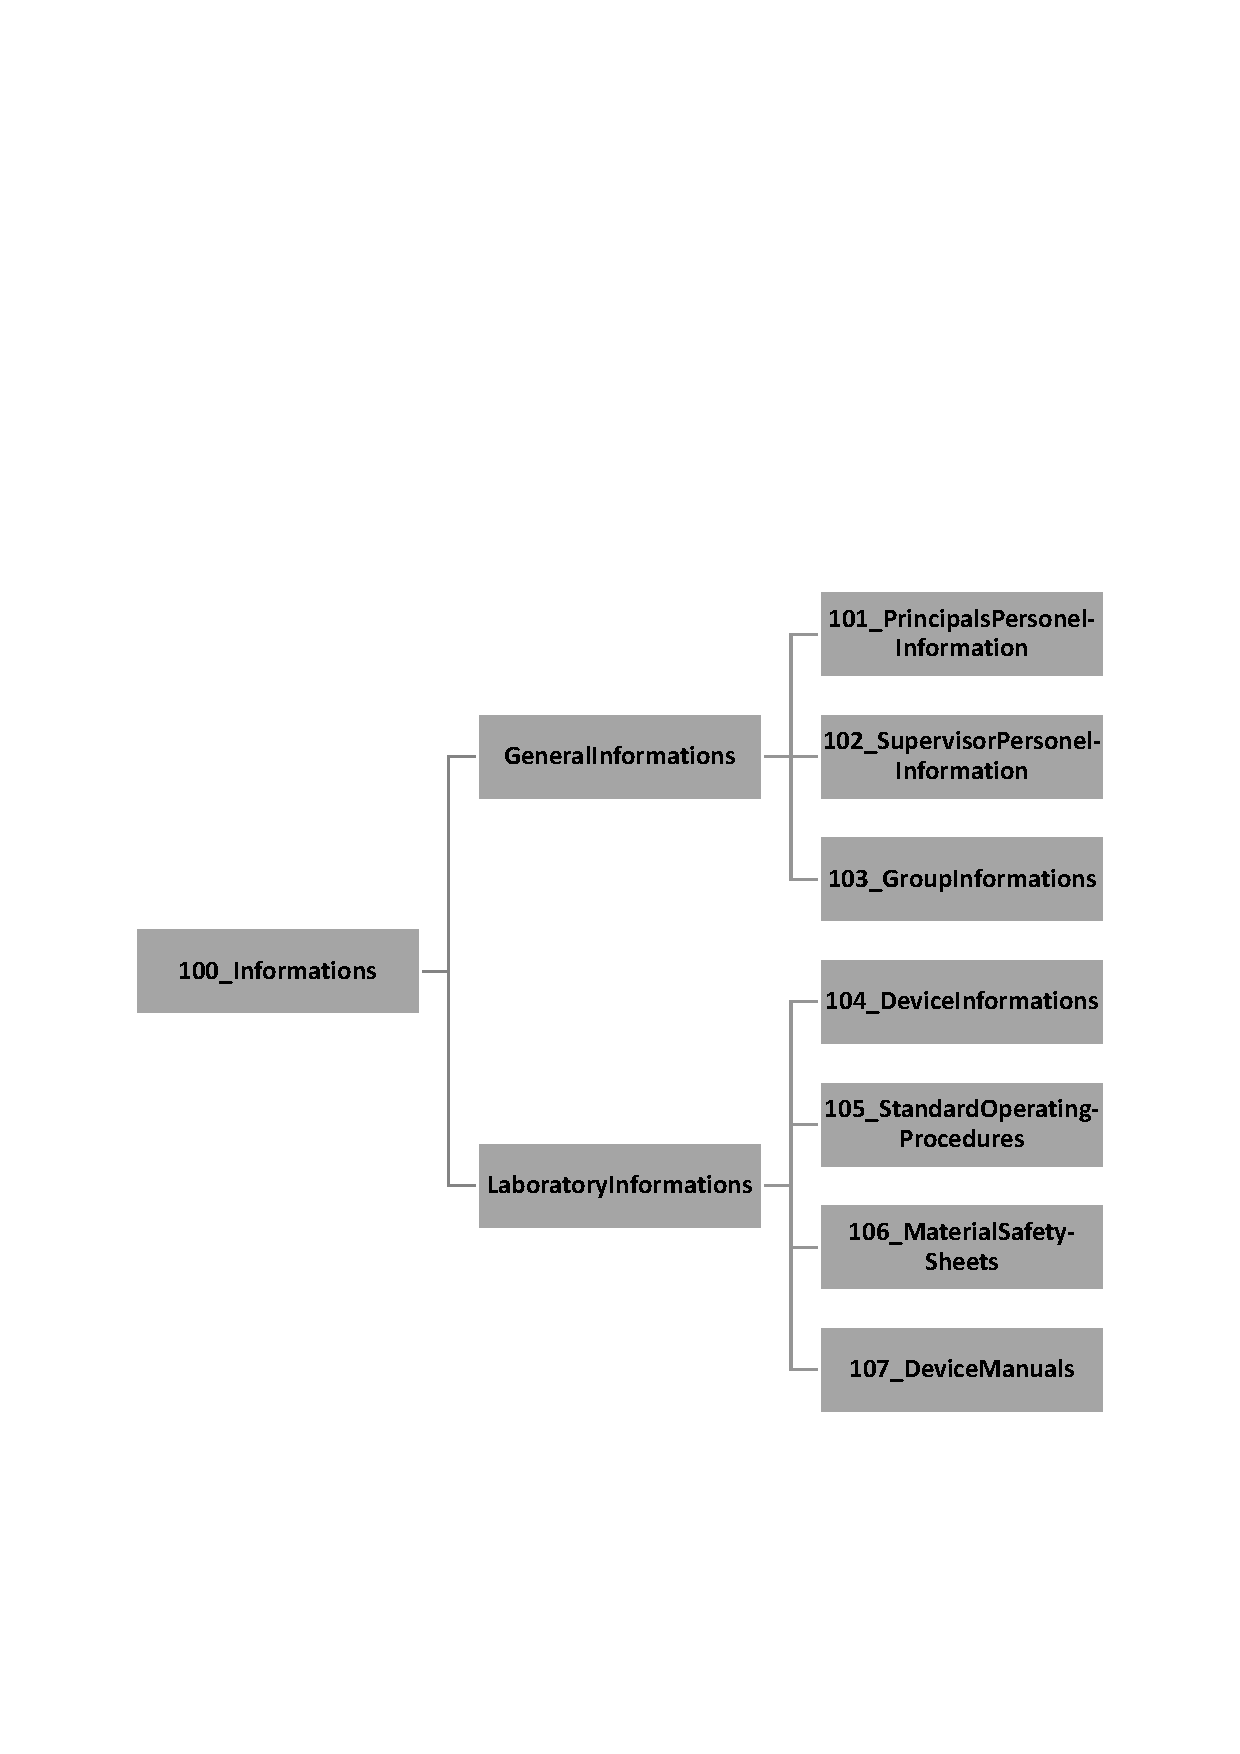
\includegraphics[width=0.9\textwidth]{Bilder/DB/ISA-S95_100_Informations.pdf}
\vspace{0em}
 \caption[100\_Informations, angelehnt an ISA-S95 und B2MML]
 {100\_Informations, angelehnt an ISA-S95}\label{fig:100informations}
\end{figure}

Den Abbildungen \ref{fig:200process} und \ref{fig:300trials} im Anhang kann die hierarchische Struktur der Rubriken 200\_ProcessEngineering und 300\_Trials entnommen werden.\\

Das \textit{Wold Batch Forum} hat eine Datenstruktur, mit dem Bezeichnung \textbf{B}usiness \textbf{To} \textbf{M}anufacturing \textbf{M}arkup \textbf{L}anguage (B2MML) entwickelt, auf der Basis von XML. XML-Dateien sind hierarchisch aufgegliedert. Jede XML- bzw. XSD-Datei (Dokument) besteht aus einem Wurzelelement (\textit{engl. rootelement}).  An dieser Stelle ist anzumerken, dass XML-Datenbanken dokumentbasiert funktionieren und hierarchische Strukturen aufweisen \cite{Verstehen2020}. Ein B2MML und BatchML Dokument (auf der Basis von XML) einer \textit{Rubrik} enthält demnach alle Informationen für eine bestimmte \textit{Rubrik}. B2MML bildet Geschäftsprozesse ab. Mit den B2MML und BatchML Vorlagen sind Unternehmen in der Lage ein individuelles Manufacturing Excecution System (MES) zu erstellen.\\

\begin{figure}[h!] %[htbp!] 
\centering
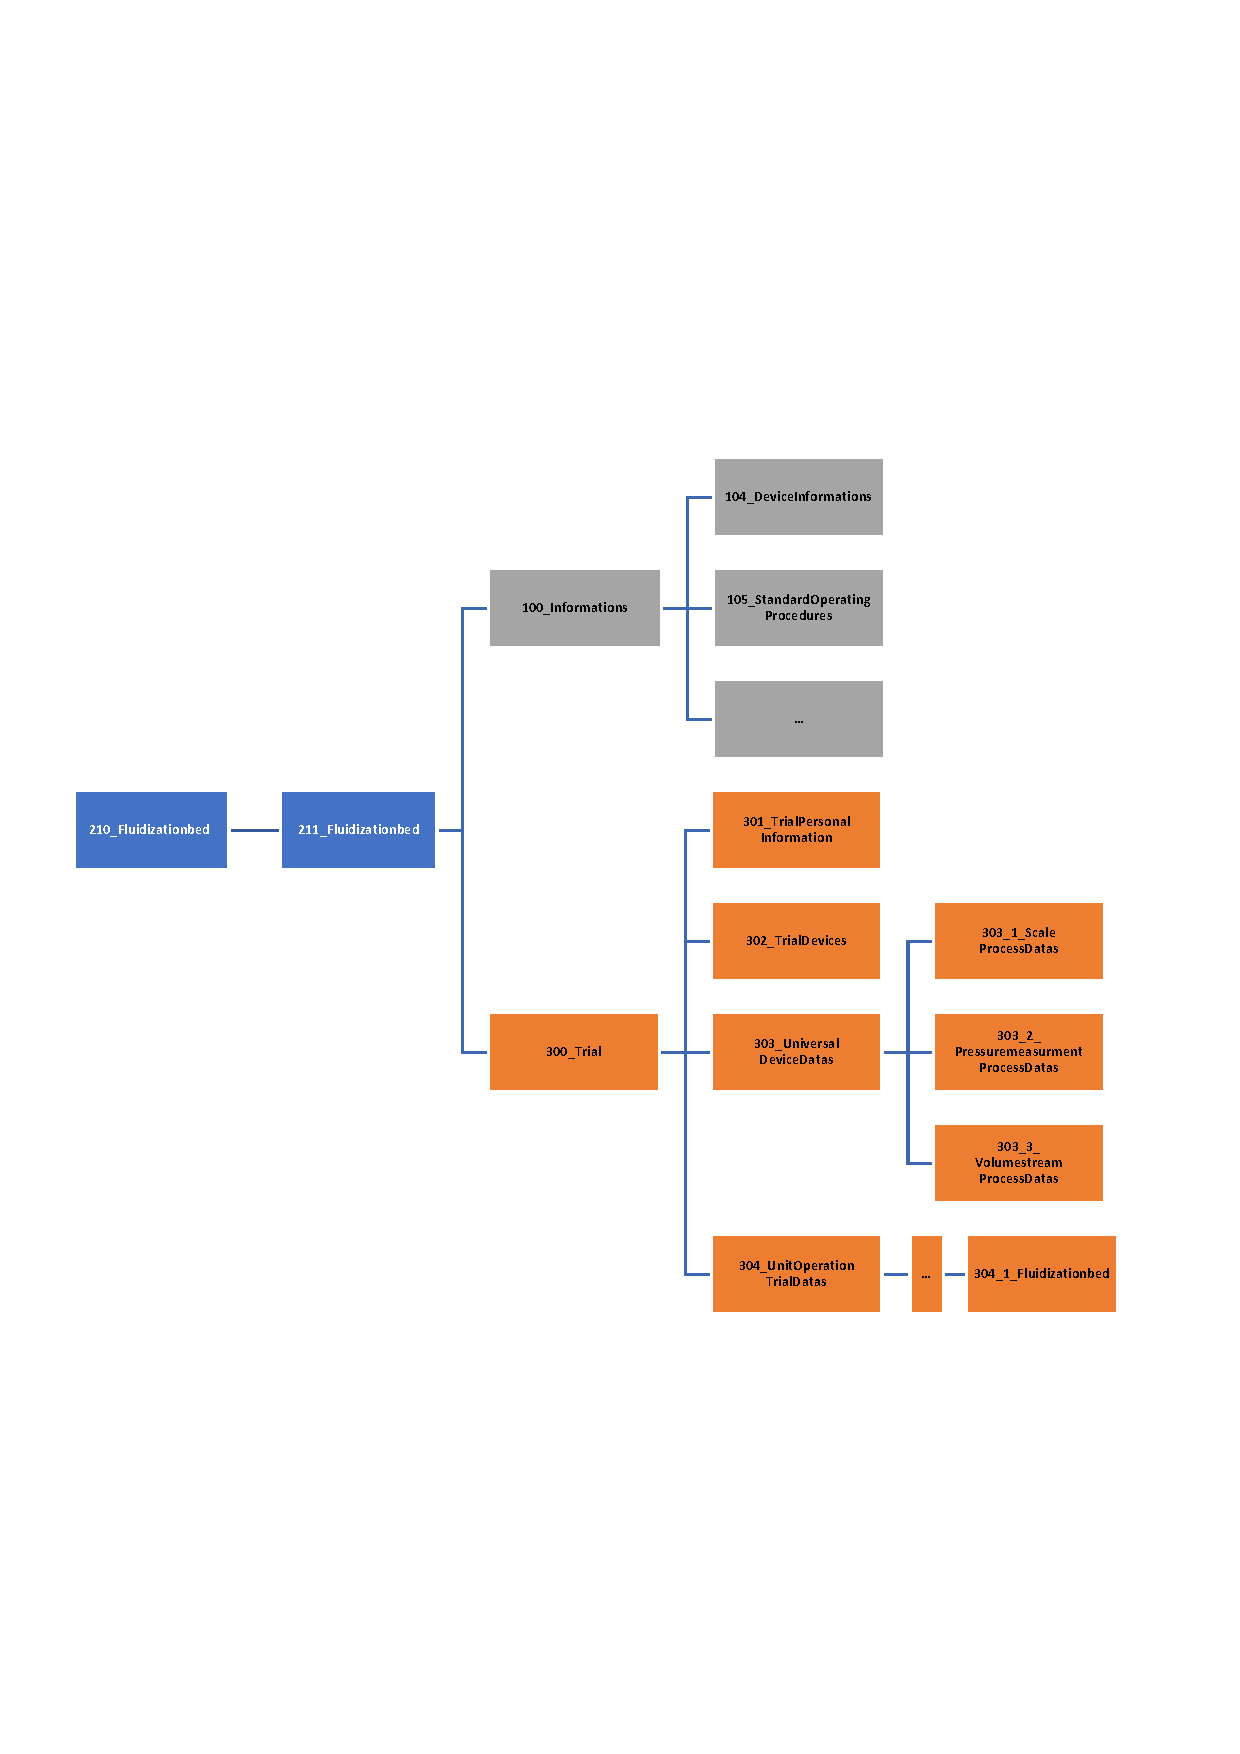
\includegraphics[width=1.05\textwidth]{Bilder/DB/wirbelschicht_hierarchisch_2.pdf}
\vspace{0em}
 \caption[Potentielle hierarchische Datenstruktur der Wirbelschicht (\textit{engl. fluidizationbed}) Unit Operation, angelehnt an ISA-S95 und B2MML]
 {Potentielle hierarchische Datenstruktur der Wirbelschicht (\textit{engl. fluidizationbed}) Unit Operation, angelehnt an ISA-S95 und B2MML}\label{fig:wirbelschicht hierarchisch}
\end{figure}

Wird das hierarchische Konzept auf das verfahrenstechnische Labor transferiert, dann könnte eine \textit{Rubrik} die Unit Operation Wirbelschicht (\textit{engl. fluidization bed}) sein. Die Struktur eines B2MML-Dokuments, zur Beschreibung eines \textbf{Wirbelschichtversuchsdurchlaufs}, könnte eine ähnliche Datenstruktur wie in Abbildung \ref{fig:wirbelschicht hierarchisch} dargestellt aufweisen. Daraus folgt, dass jeder Versuchstag bzw. Versuchsdurchlauf ein eigenes B2MML- bzw. XML-Dokument erhält. Gemäß Abbildung \ref{fig:wirbelschicht hierarchisch} würde die Unit Operation Wirbelschicht ({\Hypatia 210}) weitere \textit{branchelements} aufweisen, wie bspw. Wirbelschichttrocknen, Wirbelschichtagglomeration etc.. Das Labor der mechanischen Verfahrenstechnik der {\Hypatia HAW Life Sciences} hat nur eine Variation der Wirbelschicht, daher ist die erste und einzige Abzweigung ({\Hypatia 210}). An dieser Stelle kommen nun alle Elemente der obersten Hierarchiestufe ({\Hypatia 100, 300}). \textit{Branchelemente} der \textit{Rubrik} ({\Hypatia 100}) sollten jedoch nur Dokumentreferenzen sein, denn eine Redundanz dieser Daten hätte keinen Nutzen, sondern nur Aufwand zur Folge. Die nächste Hierarchieebene differenziert sich weiter auf und wird spezifischer. Auf der untersten eben wird es explizit. Im Rahmen dieses Beispiels würde die unterste Hierarchieebene die folgenden Elemente labeln:

\begin{enumerate}[resume, itemsep = -.1em, leftmargin=3.5em]	
\item[{\Hypatia 301}] Personenbezogenedaten des Versuchstags
\item[{\Hypatia 302}] Daten der notwendigen Geräte 
\item[{\Hypatia 303}] Erfasst alle zu erfassenen Daten. Darunter gehören diskrete sowie kontinuierliche \mbox{Daten}.
	\begin{enumerate}[ itemsep = -.1em]
	\item[{\Hypatia 303\_1}] Wiegedaten
	\item[{\Hypatia 303\_2}] Druckmessungsdaten
	\item[{\Hypatia 303\_3}] Volumenstommessungsdaten
	\end{enumerate}
	
\item[{\Hypatia 304}] Hier werden die prozessspezifischen Parameter dokumentiert
	\begin{enumerate}[ itemsep = -.1em]
	\item[{\Hypatia 304\_1}] In diesem Fall wären es die prozesspezifischen Parameter des Wirbelschichtversuchs an dem jeweiligen Versuchsstag
	\end{enumerate}
\end{enumerate}



Die Operation mit relationalen Datenbanken, auch SQL DB genannt, gestaltet sich in vielen Anwendungsfällen einfacher. Des Weiteren sind SQL DB am weitesten verbreitet und Programmschnittstellen sind in vielen Fällen für relationale Datenbanken (DB) ausgelegt. Transferiert man das hierarchische Konzept von ISA-S95 und B2MML auf eine SQL DB, dann bildet jedes einzelne Element eine eigenständige Tabelle ab. Eine dokumentenbasierte Datenbank würde beispielsweise eine ganze Unit Operation in einem Dokument zusammenfassen (vgl. Abbildung \ref{fig:wirbelschicht hierarchisch}). In einer SQL DB beschreiben demnach viele Tabellen eine Unit Operations bzw. einen Versuchsdurchlauf. Folglich ist der Aufwand der Tabellenerstellung möglicherweise höher, jedoch ist die Erstellung der abfragen via SQL einfach zu realisieren. Daher wird das ISA-S95, B2MML Konzept auf eine relationale Struktur transferiert (vgl. \ref{fig:sql_strukturentwurf}). Die Bezeichnungen in diesem Konzeptabschnitt wurden ins englische überführt.\\
 
In der Abbildung \ref{fig:sql_strukturentwurf} ist eine potentielle Datenstruktur für eine SQL Datenbank abgebildet. Es ist zu erkennen, dass Tabellen der unterschiedlichsten Rubriken; {\Hypatia 100\_Informations, 200\_ProcessEngineering, 300\_Trials}; in einer 1:N Beziehung zu einander stehen. Diese Struktur könnte den Wirbelschichtversuch hinreichend abbilden, denn:

\begin{enumerate}[ itemsep = -.1em, leftmargin=3.5em]
\item[{\Hypatia 100\_}] Informations stehen in relation mit der Unit Operation {\Hypatia 211\_Fluidizationbed}

	\begin{enumerate}[label = $\diamond$, itemsep = -.1em]
	\item Personelle Informationen werden erfasst.
	
		\begin{enumerate}[ itemsep = -.1em, leftmargin=2.5em]
		\item[{\Hypatia 101}] Auftraggeber (Professoren und Dozenten)
		\item[{\Hypatia 102}] Wissenschaftliche Mitarbeiter 
		\item[{\Hypatia 103}] Gruppeninformationen \\
		\end{enumerate}
		
	\item Allgemeine Informationen werden erfasst. Dateipfadreferenzen können hinterlegt werden. An dieser Stelle könnte eine dokumentenbasierte Datenbank Ihre Anwendung finden und die Archivierungsaufgabe besser lösen als eine SQL DB
	
		\begin{enumerate}[ itemsep = -.1em, leftmargin=2.5em]
		\item[{\Hypatia 104}] Geräteinformationen könnten sich auch Dokumentenbasiert abbilden lassen
		\item[{\Hypatia 105}] Versuchsanweisung (Standard Operating Procedures) 
		\item[{\Hypatia 106}] Materialdatenblätter
		\item[{\Hypatia 107}] Betriebsanweisungen von Geräten und Anlagen
		\item[{\Hypatia 108}] Geometrische Daten von Versuchsanlagen und Komponenten könnten Dokumentenbasiert möglicherweise effizienter archiviert werden. Eine Möglichkeit via SQL ist es für jedes Komponent eine Tabelle zu generieren. Dokumentenbasiert würde ein Bauteil ein Dokument erhalten und alle Komponenten enthalten.
		
	\end{enumerate}
	\end{enumerate}
\end{enumerate}
\pagebreak



\begin{enumerate}[resume, itemsep = -.1em, leftmargin=3.5em]	
\item[{\Hypatia 300\_}] Trials werden via diverser Tabellen erfasst
	\begin{enumerate}[ itemsep = -.1em]
	\item[{\Hypatia 300}] könnte organisatorische Daten die versuchstagbezogen sind, wie bspw. das Datum oder der wievielte Versuch (sollte eine Gruppe mal gescheitert sein), aber auch das Hochladedatum sowie eine Speicherortreferenz erfassen. Für die Speicherung der Protokolle könnte ebenfalls ein dokumentenbasierte DB Lösung zum Einsatz kommen.
	\item[{\Hypatia 301}] Personenbezogene Informationen pro Versuchstag werden erfasst
	\item[{\Hypatia 302}] könnte bei redundanten Apparaten, Geräten, Aggregaten relevant sein
	\item[{\Hypatia 303}] Erfasst alle zu erfassenen Daten. Darunter gehören diskrete so wie kontinuierliche \mbox{Daten}.
	
	\begin{enumerate}[ itemsep = -.1em]
	\item[{\Hypatia 303\_1}] Wiegedaten
	\item[{\Hypatia 303\_2}] Druckmessungsdaten
	\item[{\Hypatia 303\_3}] Volumenstommessungsdaten
	
		\begin{enumerate}[label=--, itemsep = -.5em]
		\item An der Stelle können diveser Kommentarfelder eingefügt werden, die einen Versuch beschreiben wie Subjektive Beobachtungen, die Wirbelschichthöhte und die Wirbelschichtporösität.
		\end{enumerate}
	\item[{\Hypatia 304\_1}] Hier werden die prozessspezifischen Parameter dokumentiert
	\end{enumerate}
		\end{enumerate}
\end{enumerate}

Im Anhang befindet sich eine Grafik, die verschiedene Abstraktionsebenen vermischt darstellt (siehe Abbildung \ref{fig:mixed_abstraction}). Auf der untersten Abstraktionsebene wären die expliziten Tabellen aufzufinden. Eine beispielhafte Zusammenstellung ist dem Anhang, der Abbildung \ref{fig:sql_explizit} zu entnehmen.


\begin{figure}[p!] %[htbp!] 
\centering
\vspace{-2em}
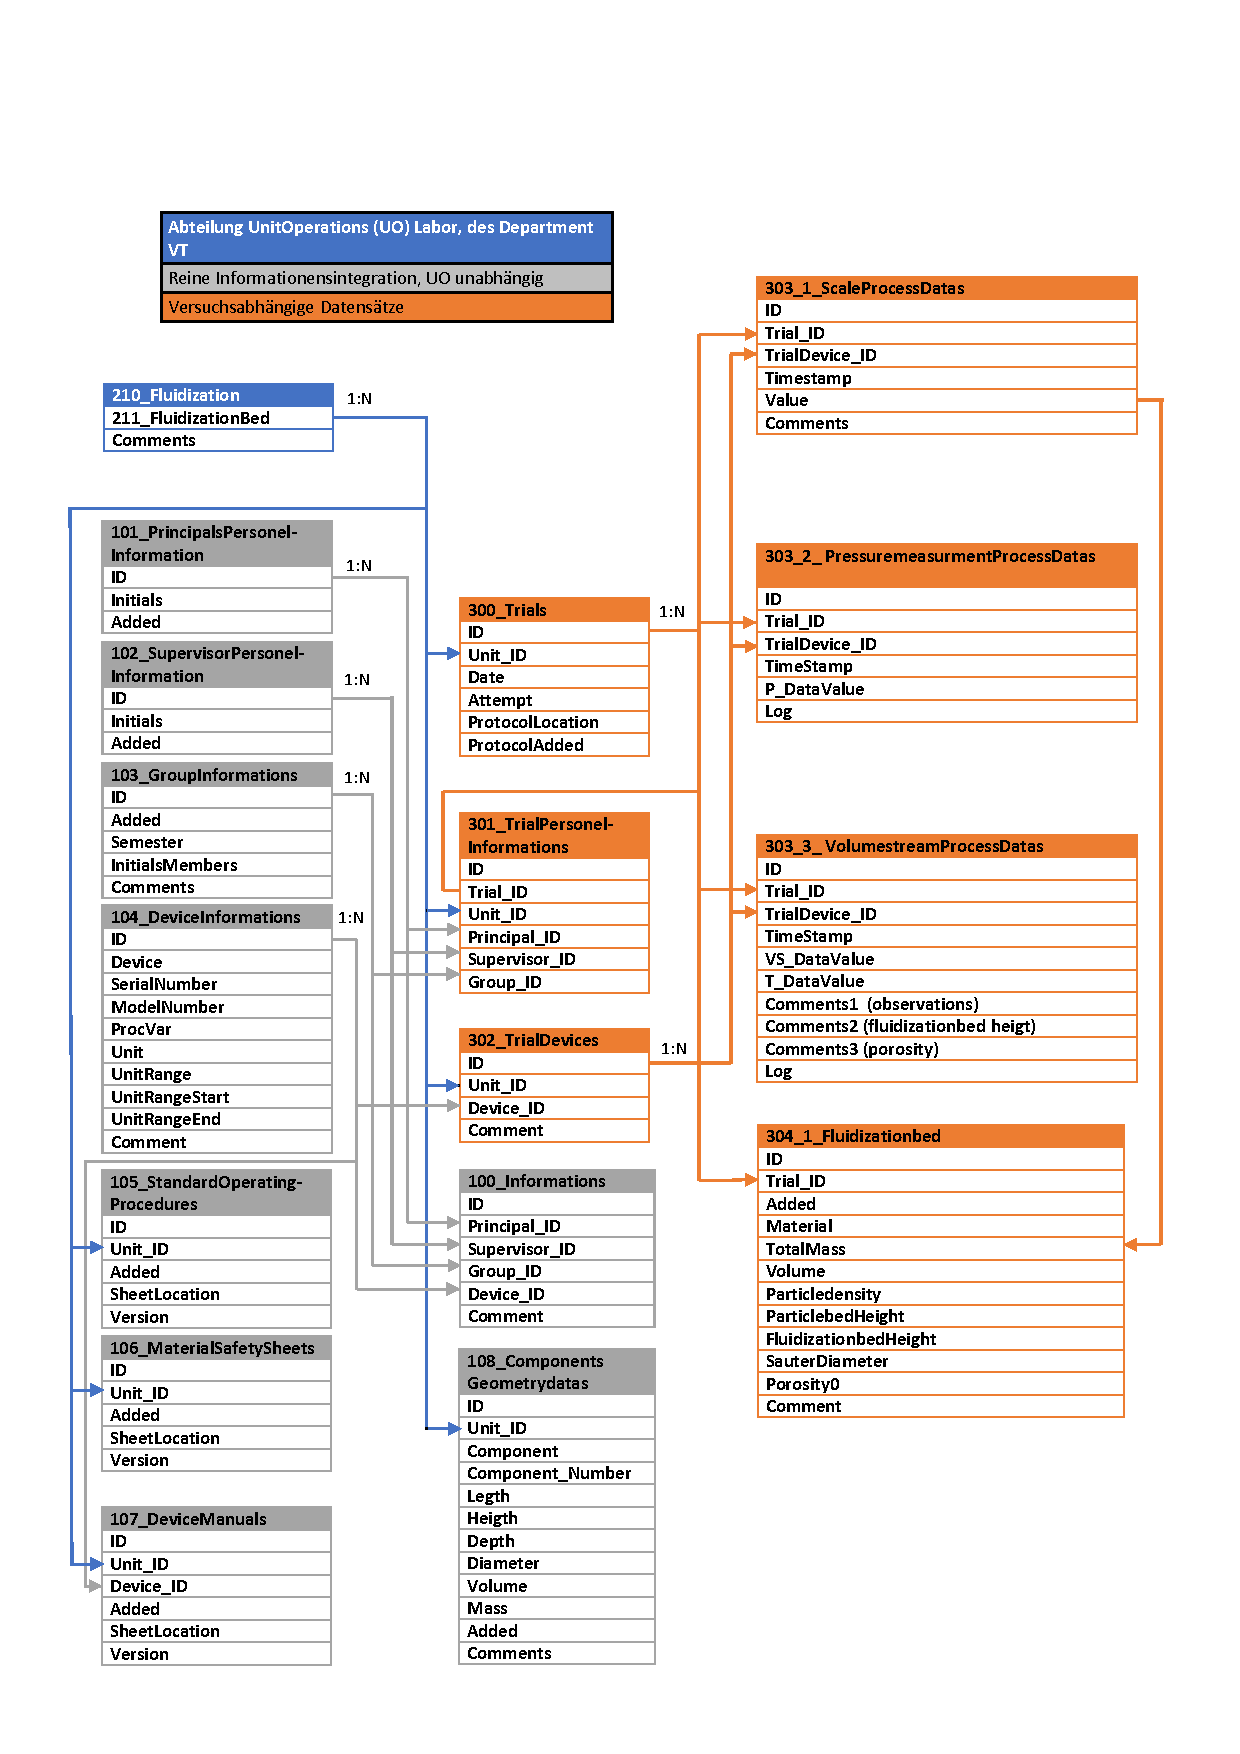
\includegraphics[width=1.02\textwidth]{Bilder/DB/wirbelschicht_sql.pdf}
\vspace{-2em}
 \caption[Datenstrukturentwurf einer relationalen Datenbank zur Beschreibung der Wirbelschicht Unit Operation, angelehnt an ISA-S95 und B2MML]
 {Datenstrukturentwurf einer relationalen Datenbank zur Beschreibung der Wirbelschicht Unit Operation, angelehnt an ISA-S95 und B2MML}\label{fig:sql_strukturentwurf}
\end{figure}

\subsubsection{Fazit}

Im Rahmen der Anwendungsfälle im Hochschulalltag könnten SQL Datenbanken den Anforderungen genügen. Das Know-How mit dieser standardisierten Datenbank Technologie ist auf andere Softwaretechnologien transferierbar. Es sollte auch möglich sein, die Erstellung einer Datenbank, im Rahmen studentischer Arbeiten, zu delegieren. Des Weiteren ist auch im Verlauf des \textit{Digitalisierungsprozess} eine Hybridlösung denkbar. 
\section{Signal- und Datenverarbeitung von Mess\-einrichtungen}

Datenerfassung oder auch Datenakquisition (\textit{engl. data acquisition}) wird häufig DAQ abgekürzt. In den folgenden Abschnitten wird die DAQ mittels
\begin{align*}
\mathrm{integrierter\,Messdatenerfassung\,}  &\textrm{via}\, \textbf{RS-232\,} \mathrm{Schnittstelle}, \\
\mathrm{analog\,Signalumwandlung\,mittels\,} \textbf{NI-USB\,6001\,} \mathrm{Messkarte\,} &\textrm{via}\, \textbf{USB\,}\mathrm{Schnittstelle}
\end{align*} 

unter der Verwendung von LabVIEW (2018, 2020 und 2021) erläutert. Für die Umsetzung wurden Anforderungen definiert, die wie folgt aufgelistet sind:

\begin{itemize}[leftmargin=*,labelsep=-\mylen]
\item Die Applikationen sollen eine graphische Oberfläche haben.
\item Der Aufwand für die Applikationsgenerierung soll minimal sein.
\item Die Applikationen sollen nur von ausgewählten Personal (\glqq leicht\grqq{}) anpassbar sein.
\item Die verwendete Software soll in der Lage sein, Daten der verschiedenste Versuchsstände und Geräte unterschiedlicher Hersteller abzubilden.
\item Es sollen Echtzeitgraphen generiert werden können.
\item Die verwendete Applikation soll kontinuierliche und diskrete Daten verarbeiten können.
\item Die Möglichkeit, die Daten in Zukunft direkt in eine Datenbank schreiben zu können, ist wünschenswert.
\end{itemize}


Es werden Module programmiert, mit denen kontinuierliche und diskrete Signalströme und Daten verarbeiten werden können. Somit ist es möglich, für alle Unit Operations Programme mittels LabVIEW zu schreiben. Diese diskreten Daten  können in einer separaten Datei oder als Header einer z.B. \,{\Menlo Tabulator} getrennten \glqq \,{\Menlo kontiMessungs.txt}\grqq{} Datei gespeichert werden. Man ist nicht daran gebunden als Spaltentrennzeichen (\textit{engl. delimiter}) \,{\Menlo Tabulator} zu verwenden, auch die Verwendung eines \,{\Menlo Komma} (\,{\Menlo *.csv} Datei), \,{\Menlo Semikolon} oder auch ein frei wählbares Trennzeichen ist möglich. Aufgrund der internationalen Konventionsunterschiede in Bezug auf das Dezimaltrennzeichen (ASCII \,{\Menlo '.'}, in Deutschland \,{\Menlo ','} etc.)  ist von der Verwendung eines \,{\Menlo Kommata} jedoch abzuraten.

\paragraph*{RS-232 zu USB Adapter} Wenn ein PC keine RS-232 Schnittstelle besitzt, kann ein RS-232 zu USB Adapter verwendet werden. Ein Mikroprozessor im Kabel emuliert eine RS-232 Schnittstelle. \\

\subsection{Serielle Schnittstellenkonfiguration und Signalverarbeitung von Messeinrichtungen}

In diesem Abschnitt werden virtuelle Instrumente (VI) zur Verarbeitung kontinuierlicher und diskreter Daten im ASCII Format (ASCII \,{\Menlo encoded}) programmiert, die über eine RS-232 Schnittstelle empfangen werden und die Daten verarbeitet. In der Abbildung \ref{fig:sensor_digitale_schnittstelle} ist zu erkennen, wie die hardwareseitige Datenverarbeitung im Falle eines Messgeräts mit integrierter digitaler Schnittstelle aussieht. Das Messobjekt, dass könnte bspw.. die gravimetrische Bestimmung eines Syntheseprodukts sein, wird messtechnisch mittels Sensor erfasst und transmittiert, dass im Messgerät bereits umgewandelte Signal, an einen Microcontroller (Arduino, RasPi ...), PC oder ähnliches.

\begin{figure}[h!] %[htbp!] 
\centering
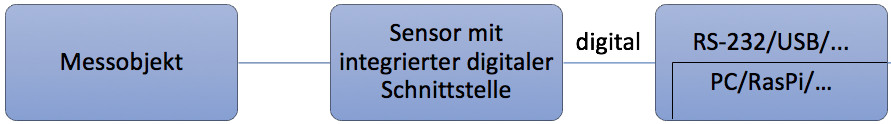
\includegraphics[width=0.9\textwidth]{Bilder/sensor_digitale_schnittstelle.jpg}
\vspace{0em}
 \caption[DAQ von Messeinrichtungen mit integrierter digitaler Schnittstelle]{DAQ von Messeinrichtungen mit integrierter digitaler Schnittstelle}\label{fig:sensor_digitale_schnittstelle}
\end{figure}

 Es werden die Schritte erklärt, wie man mit LabVIEW einen kontinuierlichen Datenstrom verarbeitet, der über eine RS-232 Schnittstelle empfangen wird. Es wird ein Windows 10 PC sowie ein Mac Book Pro und LabVIEW 2018 sowie LabVIEW 2020 verwendet, um die VI's zu programmieren und die Signale eines Messinstruments zu verarbeiten. Als Demonstrationsmesssystem wird eine Digitalwaage des Modells 440-47N des Herstellers KERN ausgelesen und die Daten interpretiert, die in eine Tabulator getrennten Text-Datei (\,{\Menlo *.txt}) geschrieben werden. Die Waage hat einen integrierten analog/digital Wandler und besitzt eine RS-232 Schnittstelle. Das Programm wird aus mehreren Sub VI's und dem Haupt VI bestehen. \\

%\begin{table}[h] % Serielle Konfigurationsparameter der Digitalwaage KERN 440-47N
%\caption{Sub VI's}
%\begin{center}
%\begin{tabular}{r|l}
%\onehalfspacing
%%\hline
%Serial Sub VI \hspace{6pt} & \hspace{6pt} Abbildung: \ref{step5} \\
%VTP Elapsed Time  \hspace{6pt} & \hspace{6pt} Abbildung: \ref{fig:vtp_elapsed_time}   \\
%Header Module \hspace{6pt} & \hspace{6pt} Abbildung: \ref{fig:modularer_header}  \\
%%\hspace{6pt} & \hspace{6pt}  \\
%
%%\hline
%\end{tabular}
%\end{center}
%\label{tab:subvis}
%\end{table}


\noindent In einem VI wird der Datenstrom, der von der Waage übermittelt wird, akquiriert. Das Sub VI wird folgend \,{\Menlo Serial Sub VI} oder in der Kurzform \textbf{\,{\Menlo SSVI}} genannt. Das \textbf{Haupt VI} wird die Daten, die es vom Sub VI erhält verarbeiten/interpretieren und in eine \,{\Menlo *.txt} Datei loggen. Des Weiteren soll das Haupt VI einen live plotter besitzen. Für einen modularen Header werden Sub VI's geschrieben, welcher Daten wie Gruppennummer, lokaler (des jeweiligen PC's) Datum- und Zeitstempel (modifizierbar), die VT Praktikums Nr. o.ä. enthält.\\

\noindent Um die korrekte Konfiguration Ihres Geräts vorzunehmen zu können, ist in dem Handbuch des Geräts nach folgenden Parametern zu schauen:

\begin{itemize} % RS-232 Parameter
\singlespacing
\item Zeichen Codierung, z.B. 7-\,{\Menlo Bit} 'ASCII'
\item \,{\Menlo Baudrate}
\item \,{\Menlo Paritätsbit}
\item \,{\Menlo Stopbit}
\item \,{\Menlo Flow Control}  (\textit{engl. dt. Flusssteuerung})
\end{itemize}

\noindent Die Digitalwaage sendet ihre digitalen Signale über eine RS-232 Schnittstelle, die 8-\,{\Menlo Bit} ASCII-encodiert sind. Um einen \textbf{kontinuierlichen Datenstrom} zu erhalten und somit \textbf{kontinuierlich} zu wiegen, wird in der Einstellung der Waage \glqq automatisches Senden\grqq{} eingestellt (das Gewicht soll gesendet werden, auch wenn der Wert nicht stabil ist). Die seriellen Konfigurationsparameter der Waage und des PC's bzw. des verarbeitenden Programms wie z.B. LabVIEW müssen identisch sein, um decodierbare Daten empfangen zu können. Diese Einstellungen sind über das Menü der Waage vorzunehmen. In der Tabelle \ref{tab:kern440} werden die verwendeten seriellen Konfigurationsparameter der Waage 440-47N des Herstellers Kern aufgelistet (Kurzschreibweise in  (\textit{engl. shorthand notation})).\\

\begin{table}[h] % Serielle Konfigurationsparameter der Digitalwaage Kern 440-47N
\caption{RS-232 Konfigurationsparameter der Digitalwaage Kern 440-47 N in shorthand \\ notation 8-N-1}
\begin{center}
\begin{tabular}{r|l}
\onehalfspacing
%\hline
\,{\Menlo Baudrate} in\,$\mathrm{s}^{-1}$ \hspace{6pt} & \hspace{6pt} \,{\Menlo 1200} \\
\,{\Menlo Byte}länge in \,{\Menlo Bit} \hspace{6pt} & \hspace{6pt} \textbf{\,{\Menlo 8}}  \\
\,{\Menlo Paritätsbit} \hspace{6pt} & \hspace{6pt} \,{\Menlo None (\textbf{N)}} \\
\,{\Menlo Stopbit} \hspace{6pt} & \hspace{6pt} \textbf{\,{\Menlo 1}} \\
\,{\Menlo Encoded} \hspace{6pt} & \hspace{6pt} ASCII \\
\,{\Menlo Flow-Control} \hspace{6pt} & \hspace{6pt} \,{\Menlo Software-Handshake} \\
%\hline
\end{tabular}
\end{center}
\label{tab:kern440}
\end{table}

\textbf{Anmerkung:} Für die Programmierung wurde eine Digitalwaage des Herstellers Kern des Typs 440-47 N gewählt. Das Programm wird auf andere Geräte übertragbar sein. Die einzige Anforderung ist, dass die RS-232 Parameter aufeinander abgestimmt werden.

\subsection{Serielle Schnittstelle im Betriebssystem finden und Debuggen} 

Die für den Benutzer sichtbare Benennung des RS-232 Ports unterscheidet sich zwischen den Betriebssystemen. Im Verlauf des Projekts wurde mit einem Unix (Mac Book Pro) und Windows 10 Betriebssystem gearbeitet. 

\paragraph*{Microsoft Windows} Bei der Verwendung eines Windows PC's wird der Port der seriellen Schnittstelle Com Port genannt und wird im Gerätemanager und in Programmen, wie z.B. in LabVIEW, \,{\Menlo COM 1-N} aufgelistet. 

\paragraph*{Mac Unix} Bei der Verwendung eines MACOS/Unix ist die serielle Schnittstelle im Terminal des Mac unter ~dev/tty.* und ~dev/cu.* zu finden und wird in LabVIEW \mbox{\,{\Menlo ASLR 1-N::INSTR}} genannt. \\

\noindent Um die richtigen Parameter zu identifizieren oder ob generell Signale, und wenn in welcher Form, empfangen werden kann mit einigen Tools ermittelt werden.

\paragraph{Tool zur Identifikation und Debuggen serieller Schnittstellen} Um herauszufinden ob die Konfigurationsparameter stimmen; ein Gerät Daten sendet, wie das Datenformat aussieht und ob die Daten korrekt übermittelt werden; kann man unter Windows das kostenlose Tool namens hTerm verwenden. Ein etwas weniger komfortables, jedoch vergleichbares open source Tool unter Mac oder Linux ist CoolTerm.\\

\subsection{Kontinuierliche Daten via RS-232 und LabVIEW verarbeiten}

Die grafische Programmiersprache G mit der Entwicklungsumgebung LabVIEW ist in der Lage Daten via RS-232 Schnittstelle zu akquirieren und zu interpretieren. Um eine serielle Schnittstelle in LabVIEW auslesen zu können, wird der \textbf{NI-VISA} Treiber benötigt. 

\footnotesize \singlespacing

 \noindent \textbf{Anmerkung:} Es werden unter MACOS einige Funktionen nicht unterstützt, wie unter anderem der LabVIEW Paketmanager und einige Pakete wie bspw. DAQmx für den Mac zu erhalten und zu implementieren hat \glqq Potentiall\grqq{}.

\normalsize \onehalfspacing


\subsubsection{Anpassung der LabVIEW-Einstellungen}
\label{sec:LabVIEW_Einstellungen}

Damit Texteingaben in Eingabefenstern (\textit{Control} Fenster) mit der Betätigung von Enter quittiert werden, ist in den LabVIEW Einstellungen folgender Haken zu setzen:

\begin{center}  % Tools > Options... > Category > Enviroment > End text entry ...
Tools > Options ... > Category > Enviroment > End text entry with Enter key [aktivieren]
\end{center} 

\noindent Wenn ein serieller Port geöffnet wird \textbf{ist es wichtig, dass bei dem Beenden des Programms der serielle Port geschlossen wird!} Wenn der Abbruch Button (\textit{engl. abort button}) von LabVIEW genutzt wird, wird der Port nicht geschlossen, daher soll das VI nur über den \textit{Stop Button} des Frontpanels geschlossen werden. Um den \textit{Abort Button} für das gerade verwendete VI (Programm) zu entfernen, gehen Sie bitte wie folgt vor:

\begin{center} % File > VI properties... > Window Apperance > Customize ...
File > VI properties > Window Apperance > Customize ... >  Show Abort button [deaktivieren]
\end{center} 

\input{Benötigte_LabVIEW_Objekte}
 
\subsubsection{Serielle Sub VI programmierung}

Zu Beginn wird ein VI oder wie auch nachfolgend \textit{Objekt} genannt programmiert (in LabVIEW auf englisch \textit{Function}). Dieses VI wird im folge Abschnitt in das Haupt VI als Sub VI mit dem Namen \textit{Serial Sub VI} integriert. Zu Beginn öffnet man ein neues leeres VI. Das \textit{Serial Sub VI}, im folgenden \textit{SSVI}, wird für die Konfiguration einer seriellen Schnittstelle verwendet. Die von LabVIEW verwendeten \textit{Objekte} können Sie den Tabellen \ref{tab:labviewserialobject} und \ref{tab:labviewserialobject2} entnehmen. In den Tabellen \ref{tab:labviewserialobject} und \ref{tab:labviewserialobject2} (die sich ebenfalls im Anhang befinden), sind alle Objekte aufgelistet die benötigt werden, um die \textit{VI's} zu programmieren. In den Tabellen \ref{tab:labviewserialobject} und \ref{tab:labviewserialobject2} wird das Blockdiagramm mit \textbf{BD}, das Front Panel mit \textbf{FP} und die rechte Maustaste mit \textbf{rM} abgekürzt. In den folgenden Programmierabbildungen sind die Funktion wie in den Tabellen \ref{tab:labviewserialobject} und \ref{tab:labviewserialobject2} nummeriert.\\

\paragraph{Erster Schritt: Serielle Objekte} Nach dem Erstellen eines neuen VI's fügt man alle Objekte ein, die man für den Datentransfer mit serieller Schnittstelle benötigt (4 - 9 in Tabelle \ref{tab:labviewserialobject}) (siehe Abbildung \ref{step1}). 

\bildp{h!}{1}
{LabVIEW_serialport/step_1_all_serial_functions_2.png}
{0em}
{Einfügen aller seriellen Funktionen}
{Einfügen aller seriellen Funktionen}
{step1}


\paragraph{Zweiter Schritt: Port Initialisierungs- und Abbruchskonfiguration} An dem Objekt \,{\Menlo Configure Port} sind Konstanten mit den Konfigurationswerten hinzuzufügen. An den Objekteingängen auf der linken Seite des Objekts, erstellt man Konstanten (rechte Maustaste/\,{\Menlo Create Constant} (11), siehe Abbildung \ref{step2}), die die seriellen Konfigurationsparameter enthalten (siehe Tabelle \ref{tab:kern440}). Um den Anwender dieses VI's den gesamten Kombinationsraum der Parameter zu Verfügung zu stellen, ist es auch möglich anstelle der Konstanten, \,{\Menlo Controls} zu verwenden. Anschließend zieht man eine \,{\Menlo Case-Structur} (2a) um das \,{\Menlo Configure Port} (zzgl. Konstanten) sowie das \,{\Menlo Flush Buffer} (9) Objekt und eine weitere \,{\Menlo Case-Structur} (2b) um das \,{\Menlo Close Port} Objekt. Wird die \,{\Menlo Case-Structure} (29) mittels eines Wahrheitswerts (\textit{boolean variable}, \,{\Menlo true}/\,{\Menlo false}) getriggert, wird somit der Port Konfiguriert und der I/O Buffer \textit{geflushed}. Die \,{\Menlo Case Structure} (2b), auf der rechten Seite wird mittels eines \,{\Menlo Stop Buttons} auf \,{\Menlo true} gestellt, um den Port mittels des \,{\Menlo Close} (8) Objekts zu schließen.\\

\noindent Den Stop \textit{Button} (14), die \textit{VISA ressource name} (13) zur Auswahl des Ports und den String \textit{Indicator} (12) (siehe Tabelle \ref{tab:labviewserialobject}, 12 - 14) fügt man z.B. über das Front Panel hinzu und positioniert die dazugehörigen Objekte, die automatisch im Blockdiagramm erscheinen, an der richtigen Positionen. Der \textit{Stop Button} wird mit dem \textit{Case Selektor} der zweiten \textit{Case-Structure} (2b) verbunden. Wird das Programm durch diesen \textit{Stop Button} beendet, wird somit der Port geschlossen. \textbf{Aufgrund dessen ist es wichtig, den VI Abbruch Button zu Deaktivieren: \emph{File > VI properties... > Window Apperance > Customize ... > [Markierung entfernen] Show Abort button}}. Ein \textit{Indicator} zum Anzeigen und zum weiterreichen des, durch das \textit{Read} Objekt (6) ausgelesenen Strings, wird an das \textit{Read} Objekt (6) angeschlossen. Die erste \textit{Case Structure} (2a) wird durch ein \textit{First Call?} (3) Objekt getriggert.\\

\begin{figure}[hp!]
\subfloat
	[Einfügen von Stop Button, Indicators und VISA resource]
	[Einfügen von Stop Button, Indicators und VISA resource \label{step2}]{
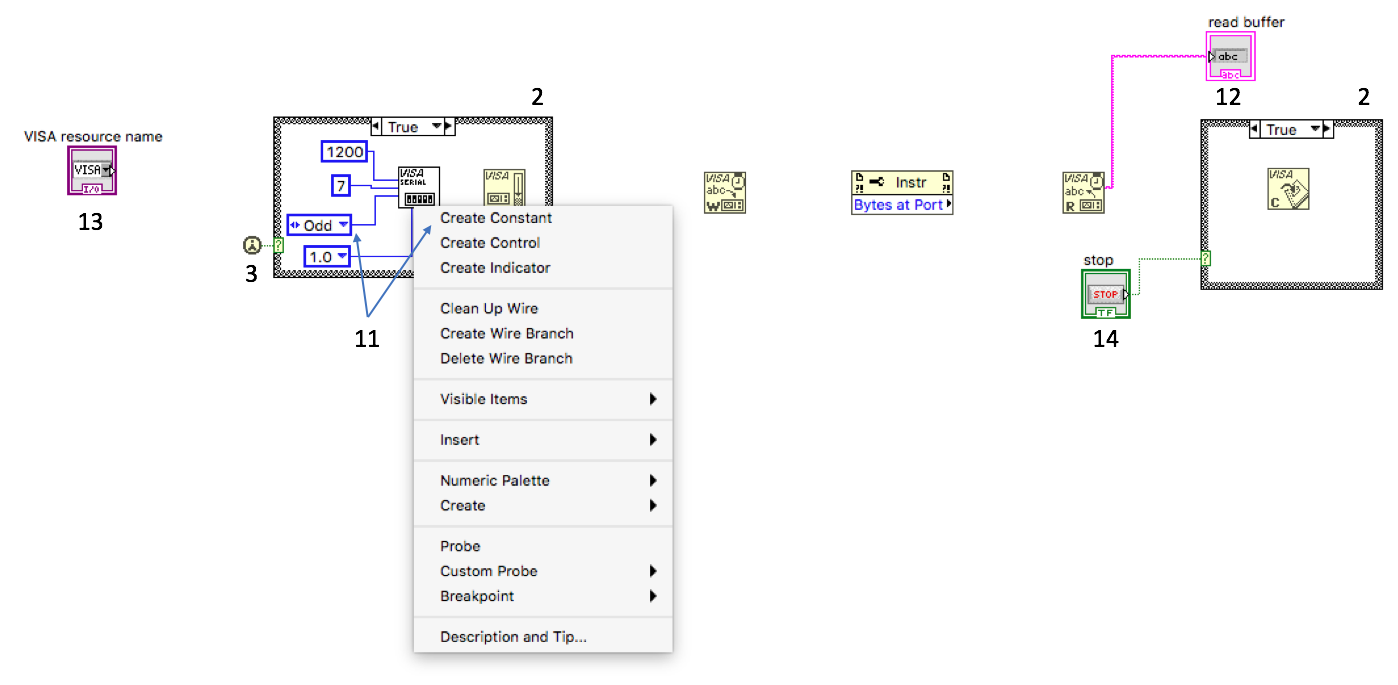
\includegraphics[width=1\textwidth]
	{Bilder/LabVIEW_serialport/step_2_cases_buttons-indicators-controls_2.png}
}
\phantomcaption
\vspace{5pt}
\ContinuedFloat
\subfloat
	[Einfügen von For Loop und Schieberegister]
	[Einfügen von For Loop und Schieberegister\label{step3}]{
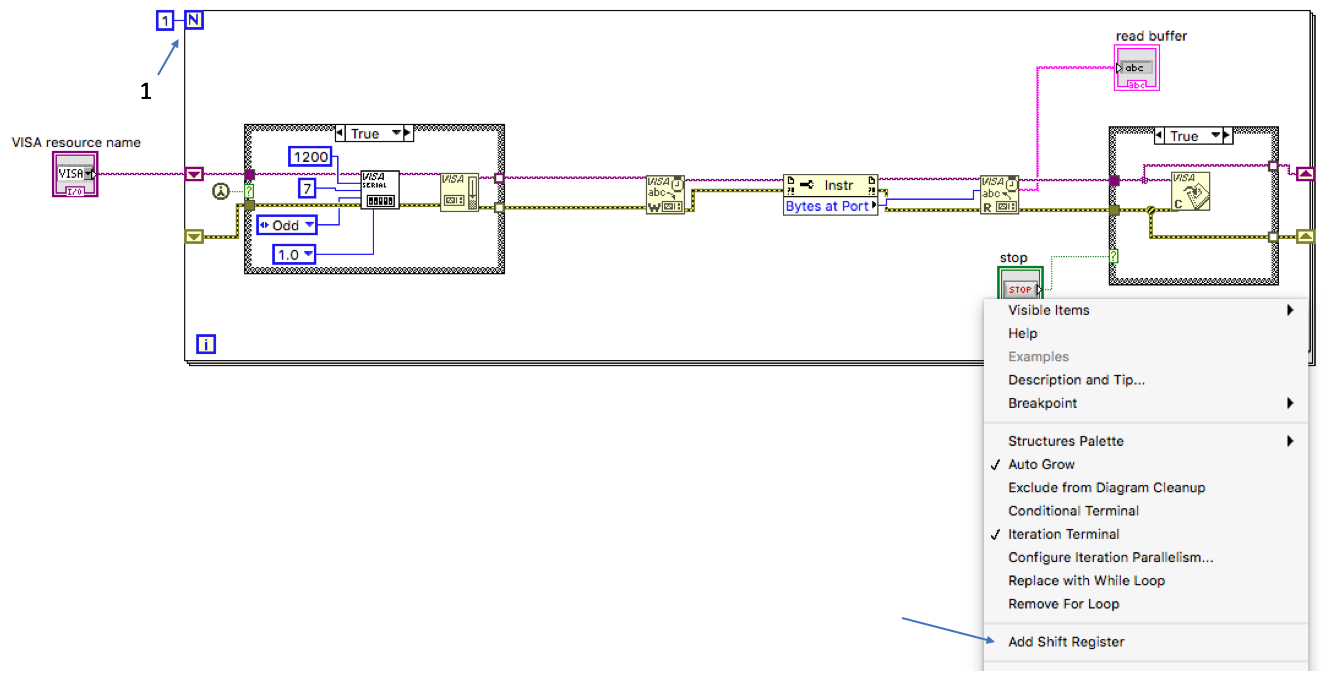
\includegraphics[width=1\textwidth]
	{Bilder/LabVIEW_serialport/step_3_for-loop_add-shift-register_2.png}
} 
\caption[]{Einfügen von Stop Button, Indicators, VISA resource, For Loops und Schieberegister}
\label{fig:step2_step3}
\end{figure}


\paragraph{Dritter Schritt: N = 1 For Loop, XON flow control}

Nun zieht man ein eine \,{\Menlo For} \,{\Menlo Loop} um alle Objekte, bis auf die \,{\Menlo VISA} \,{\Menlo Resource} und das \,{\Menlo Flush Buffer} Objekt. Die {\,{\Menlo For} \,{\Menlo Loop} wird in diesem Fall mit der Konstante 1 initialisiert (siehe Abbildung \ref{step3}, oben links). Nach dem hinzufügen von zwei Schieberegistern (\textit{engl. Shift Register}), sind alle Objekte wie in Abbildung \ref{step3} zu verdrahten. Durch das Hinzufügen eines \,{\Menlo Shift Registers} an einem Ende einer \,{\Menlo For Loop} oder \,{\Menlo While Loop}, werden automatisch die \,{\Menlo Shift Register} auf der anderen Seite des Loops generiert. Alle Funktionen müssen nun, wie in Abbildung \ref{step3}, verbunden werden (die blaue Leitung zwischen \,{\Menlo Bytes at Port} und \,{\Menlo Read Port} ist ebenfalls zu verbinden). Da die \glqq Verkabelung\grqq{} im \,{\Menlo true} Case beider \,{\Menlo Case Structures} verkabelt sind, muss selbiges noch im \,{\Menlo false} Case beider \,{\Menlo Case Structures} (2ab) geschehen (siehe Abbildung \ref{step3b}). Das \,{\Menlo Write} Objekt (7) ist mit der String Konstante (10) mit dem Wert \,{\Menlo 11} zu verknüpfen. Die \,{\Menlo String Konstante} \,{\Menlo 11} beinhaltet das ASCII flow control (siehe Abschnitt RS-232) Signal XON und signalisiert der Waage, dass der PC bereit ist Daten zu empfangen, da die Waage als \,{\Menlo flow control} den Software-Handshake verwendet. Technisch wird an die Waage der Hexadezimale \textit{character} 11 geschickt, also \,{\Menlo 0x11}. \,{\Menlo 0x11} ist das ASCII Hexadezimalzeichen für XON.  Dieses Objekt in dieser Form ist nun alleinstehend fähig den seriellen Port zu konfigurieren, der Waage das \,{\Menlo flow control} Signal XON zu senden, die Bytes auszulesen und darzustellen oder dem Haupt VI zu übergeben sowie den seriellen Port zu schließen, wenn das Programm über den Stop Button beendet wird.

\begin{figure}[h!p]
	\hfill     
     \subfloat[\glqq Verdrahtung\grqq{} der \,{\Menlo false} Cases]
     [\glqq Verdrahtung\grqq{} der \texttt{false} Cases\label{step3b}]{%
       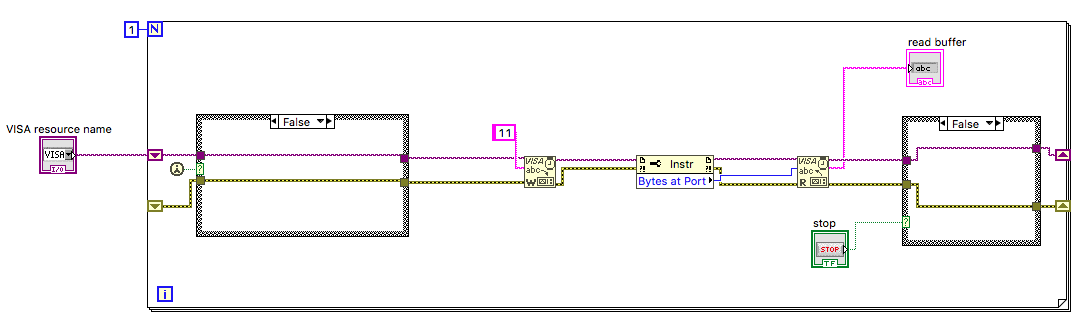
\includegraphics[width=0.99\textwidth]
       {Bilder/LabVIEW_serialport/step_3b_false_cases.png}
     }
     \phantomcaption
     \vspace{3pt}
\ContinuedFloat  
     \subfloat[Einfügen von For Loop und Schieberegister]
     [Optimiertes SSVI\label{step5}]{%
       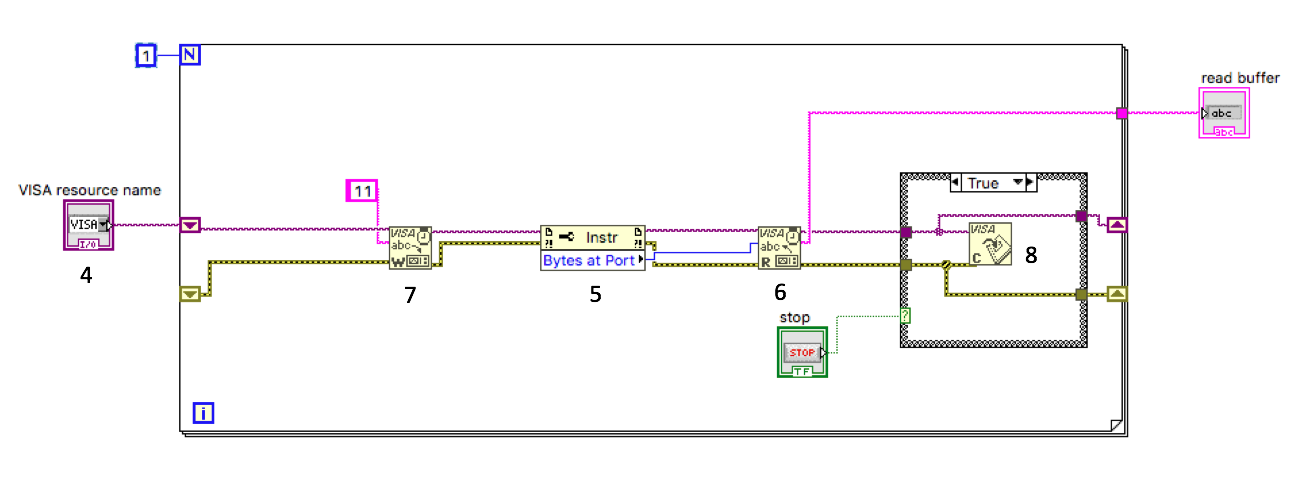
\includegraphics[width=1\textwidth]
       {Bilder/LabVIEW_serialport/step5_optimierung.png}
     }
     \caption[]{\glqq Verdrahtung\grqq{} der \,{\Menlo false} Cases und Optimiertes SSVI
  }
  \label{fig:step3b_step5}
\end{figure} % Einfügen von Stop Button, Indicators, VISA resource, For Loops und Schieberegister



\paragraph{Vierter Schritt: Optimierung} Das Programm in Abbildung \ref{step3} und \ref{step3b} konfiguriert bei jeder Iteration den Port und öffnet ihn. Das öffnen eines seriellen Ports, der bereits geöffnet ist, kann zu Störungen führen, daher sollte die Konfiguration des Ports über das Haupt-VI erfolgen. Der I/O-Buffer soll auch nur bei der ersten Iteration des Hauptprogramms gelöscht werden, der wird ebenfalls ins Haupt VI verlagert. In Abbildung \ref{step5} ist das Objekt nach der Optimierung abgebildet. Um den ausglesenen String nach Abschluss der Iteration an das Haupt VI übergeben zu können, wird der read Buffer rechts aus der For Loop geleitet. Das Objekt \,{\Menlo Configure Port} hat für den Inputbuffer per default 4096 \,{\Menlo Bytes} (Anmerkung: Sollte Ein I/O Buffer overflow o.ä. auftreten, dann könnte die Pause zwischen Iterationen zu lang sein). Mit Abschluss dieser Schritte ist das VI Objekt einsatzbereit und kann in mehrere Programmen, implementiert werden. Dafür müssen in der oberen rechten Ecke des Frontpanels die Ein- und Ausgänge des VI festgelegt werden (siehe Abbildung \ref{step4}, Nr. 16). Dazu klickt man auf ein Feld des Icons in der oberen rechten Ecke und auf eine Funktion, die sich im Frontpanel befindet. In diesem Beispiel wurde die obere rechte Ecke des mini Icons angewählt und mit einem Klick auf \,{\Menlo read buffer}, dem ausgelesenen String zugeordnet. Die obere linke Ecke des mini Icons wird mit VISA resource name und die Ecke unten links mit dem \,{\Menlo Stop Button} belegt.

\bild{.4}
{LabVIEW_serialport/step_4_VI_generieren_3.png}
{0em}
{Definition der VI Objekt Ein- und Ausgänge}
{Definition der VI Objekt Ein- und Ausgänge}
{step4}


\subsubsection{Kontinuierliche Messdatenerfassung RS-232 im Haupt VI}

Die Daten, die man via RS-232 empfängt, müssen interpretiert und in einer *.txt Datei gelogged werden. Die empfangenen Daten hängen von der verwendeten Messtechnik ab. Das Untersuchungsobjekt im Rahmen dieses Abschnitts ist eine Digitalwaage (KERN 440-47N). Das Datenformat dieser Waage ist wie folgt:

\begin{enumerate}
\singlespacing
\item Es können beliebig viele Leerzeichen zu Beginn des Strings vorhanden sein (\,{\Menlo '\textbackslash s'})
\item Es kann die Vorzeichen \,{\Menlo +} oder \,{\Menlo -} enthalten
\item Es können beliebig viele \,{\Menlo '\textbackslash s'} folgen
\item Es können beliebig viele Ziffern folgen
\item Es wird ein dezimal Trennungszeichen folgen (ASCII encodiert wäre es der Punkt \,{\Menlo '.'})
\item Es können wieder unbekannt viele Ziffern folgen
\item Es können beliebig viele \,{\Menlo '\textbackslash s'} folgen
\item Es kann die Maßeinheit \,{\Menlo 'g'} folgen, wenn der Messwert stabil ist
\item Es können beliebig viele \,{\Menlo '\textbackslash s'} folgen
\item Das Zeilenende kann je nach System variieren. Es kann \,{\Menlo '\textbackslash r'}, \,{\Menlo '\textbackslash n'}, \,{\Menlo '\textbackslash r''\textbackslash n'} oder \,{\Menlo '\textbackslash r\textbackslash n'} sein
\end{enumerate}


\paragraph{Erster Schritt: Port Konfiguration und String verketten/anzeigen lassen} Nach dem Erstellen eines neuen, leeren VI's, wird das VI des vorherigen Abschnitts per drag and drop in das leere VI gezogen. Dazu zieht man das Symbol 16 des \textit{SSVI} (siehe Abbildung \ref{step4}) in das neue VI. Als nächstes setzt man eine While Loop um dieses VI Objekt und verknüpft einen Stop Button (14) mit dem Stop Eingang des SSVI sowie dem Abbruchkriterium der While Loop (20). Außerhalb des Loops wird die Portkonfiguration (siehe Tabelle \ref{tab:kern440}) und das Objekt, welches den I/O Buffer (9) löscht, platziert. Um die Daten der Waage in Form eines Strings aus dem SSVI auszulesen, wird die Funktion zum Verketten von Strings \textit{engl. Concatenate Strings} (17) in den Loop platziert. Man benötigt Schieberegister (\textit{engl. Shift Register}), erweitert das \,{\Menlo Concatenate Strings} (17) Objekt auf zwei Eingänge und verbindet die \,{\Menlo Shift Register} mit der \textit{Concatenate Strings} (17) Funktion (links oberer Eingang des \textit{Concatenate Strings} (17) Objekts). Damit das \,{\Menlo Shift Register} bei der ersten Iteration (Index = 0, da LabVIEW, wie viele andere Programmiersprachen, 0 indexiert arbeitet) leer ist, wird das linke \,{\Menlo Shift Register} mit einer leeren String konstante gelöscht. In Abbildung \ref{step6} sind die beschriebenen Funktionen abgebildet. Um zu sehen ob und was empfangen und verkettet wird, fügen wir einen \,{\Menlo String Indicator} (21) ein. Da der Nutzer des Programms \,{\Menlo VISA Ressource} und \,{\Menlo String Indicator} sehen wird, ist es empfehlenswert es im FP in etwas eindeutiges umzubenennen. Um eindeutig erkennen zu können, welche Zeichen empfangen werden, kann man im Front Panel per rechts-klick in das entsprechende Fenster, die \,{\Menlo String Indicator} Anzeige in \,{\Menlo '\textbackslash'} umstellen (siehe Abbildung \ref{step6b}).

\bildp{h!}{0.7}
{LabVIEW_serialport/step6.png}
{0em}
{BD Haupt VI: SSVI Integration/Port Konfiguration/String\-operationen}
{BD Haupt VI: SSVI Integration, Port Konfiguration, String auslesen und \mbox{verketten}}
{step6}



\bild{0.4}
{LabVIEW_serialport/step6b.png}
{0em}
{FP Haupt VI: SSVI Integration/Port Konfiguration/String\-operationen}
{FP Haupt VI: SSVI Integration, Port Konfiguration, String auslesen und \mbox{verketten}}
{step6b}

\paragraph{Zweiter Schritt: \glqq String Slicing\grqq} Das VI verkettet den String bis zum Beenden des Programms. Um eine einzige abgeschlossene Zeichenkette (von String Beginn bis \,{\Menlo '\textbackslash n'}) zu erhalten, müssen wir den String kürzen (\textit{engl. slicing}). Dazu wird eine \,{\Menlo Case Structure} (2c) programmiert, die den String verkettet, bis die \,{\Menlo Search/Split String} (23) Funktion das von uns gesuchte Zeichen, das ASCII Steuerzeichen \,{\Menlo '\textbackslash n'} liest. Es können zwei Zustände vorliegen, \,{\Menlo true} und \,{\Menlo false}. 

\begin{quote}
Anmerkung: Bei der Funktion \,{\Menlo Configure Port} (4) ist per default \textit{Termination Character} auf \,{\Menlo true} gesetzt, was dazu führt, dass \,{\Menlo Read} (6) des SSVI beim decodieren der bytes, die sich im Input Buffer des Serial Ports befinden, beim decodieren des Steuerzeichens  \,{\Menlo '\textbackslash n'}, die Zeichenkette terminiert und alle weiteren Bytes, die sich im Input Buffer befinden, in der nächsten Iteration bis maximal zu einem \,{\Menlo '\textbackslash n'} gelesen und decodiert werden.
\end{quote}


\paragraph*{false} Die \,{\Menlo Search/Split String} Funktion soll nach einem \,{\Menlo '\textbackslash n'} Suchen. Der \textit{offset of match} Ausgang der Funktion gibt den Index des Matches im String an. Wenn die \,{\Menlo Search/Split String} Funktion das zu suchende Zeichen (in dieser Situation \,{\Menlo  '\textbackslash n'}) nicht findet, gibt \textit{offset of match} -1 wieder. Diese Information wird genutzt, um den \textit{Case Selektor} auf \texttt{false} zu setzen. 

Wenn der String kein \,{\Menlo '\textbackslash n'} enthält, gibt die Funktion als \,{\Menlo offset of match} den Index -1 zurück, demnach ist das boolsche Signal \texttt{true} aus der \,{\Menlo Equal?} (26) Funktion. Dieses Signal wird mit dem boolschen Operator \,{\Menlo Not} (27) negiert. Der \,{\Menlo Case Selector} (24) ist somit auf \,{\Menlo false} gesetzt.\\
Ist der \,{\Menlo Case Selector} (24) auf \,{\Menlo false}, wird der Draht, der den verketteten String (\,{\Menlo Shift Register} und \,{\Menlo SSVI}) enthält, in die \,{\Menlo Case Structure} (2c) geleitet und mit dem rechten \,{\Menlo Shift Register} verbunden.\newline

\noindent An dieser Stelle (siehe Abbildung \ref{slicing_bedingung}) wird nun eine \textbf{Sicherheit} eingebaut. Der String soll erst interpretiert werden, wenn die Länge des Strings größer einer Vorgabe ist. Die Länge einer Zeile kann dem Handbuch des jeweiligen Geräts entnommen werden oder sie wird durch das manuelle \textit{Debugging} z.B. hTerm oder trial and error eruiert. 


\begin{figure}[h!] 
\centering
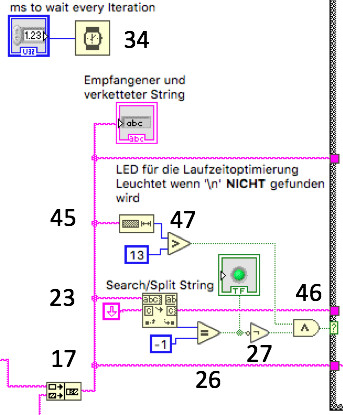
\includegraphics[width=0.4\textwidth]{Bilder/LabVIEW_serialport/slicing_bedingung.jpg}
\vspace{2pt}
\caption[Slicing Bedingung]{Slicing Bedingung}\label{slicing_bedingung}
\end{figure}

\paragraph*{true} Wenn der String \,{\Menlo '\textbackslash n'} enthält, gibt \textit{offset of match} dem \,{\Menlo Search/Split String} (23) Objekt den Index an, wo das Zeichen (in diesem Fall \texttt{'\textbackslash n'}) im String gefunden wurde. Der ist ungleich -1, der boolsche Zustand ist somit \,{\Menlo false} und wird mit der \,{\Menlo Not} (27) Funktion wieder in ein \,{\Menlo true} umgewandelt. Der \,{\Menlo Case Structure Selector} (24) ist damit auf \,{\Menlo true} gesetzt. Nun soll der Folgeiteration der Teil des Strings ab dem gesuchten Zeichen übergeben werden. Das kann mithilfe des Objekts \,{\Menlo String Subset} erreicht werden, indem man den Rest des Strings, des Objekts \,{\Menlo Search/Split String} (23), im \,{\Menlo true} Case, dem Objekt \,{\Menlo String Subset} (25) übergibt. Das Objekt \,{\Menlo String Subset} (25) wird die Konstante 1 der Funktion \textit{offset} zugewiesen. Durch diese Konfiguration der Funktionen wird der Rest des Strings \textbf{nach} dem gesuchten Zeichen (\,{\Menlo '\textbackslash n'}) dem \,{\Menlo Shift Register} (19) übergeben. Ist der PC und das Programm schneller als die empfangenen Daten, dann ist der übergebene String leer.

% \bild{1}
%{LabVIEW_serialport/step7_stringslicing.jpg}
%{-1em}
%{\glqq String Slicing\grqq{}: Dateninterpretation}
%{\glqq String Slicing\grqq{}: Dateninterpretation}
%{step7}

\begin{sidewaysfigure}
    \centering
    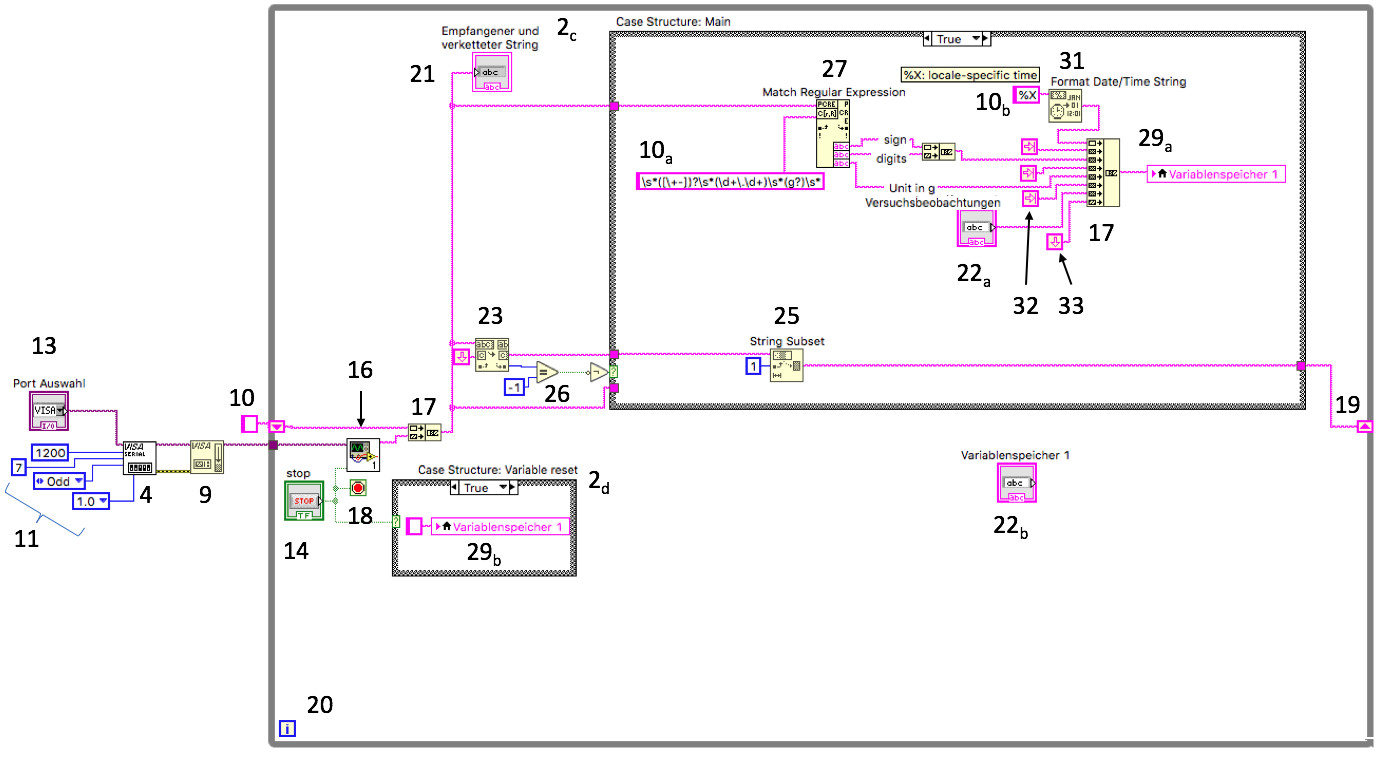
\includegraphics[width=1.04\textwidth]{Bilder/LabVIEW_serialport/step7_stringslicing.jpg}
    \caption[\glqq String Slicing\grqq{}: Dateninterpretation]{\glqq String Slicing\grqq{}: Dateninterpretation}
    \label{step7}
\end{sidewaysfigure}

\paragraph{Dritter Schritt: \glqq Dateninterpretation\grqq{}} Sobald eine vollständige Zeichenkette gelesen wurde, müssen die Daten in ihre Bestandteile zerlegt werden (siehe Abbildung \ref{step7}). In der \,{\Menlo Case Structure} (2c) wird im \,{\Menlo true}\, Case mit dem Objekt \,{\Menlo Regular Expression Match} (28), aus dem gesamten vorgelegten String alle gewünschten und potentiell vorkommenden Ausdrücke (\textit{engl. expressions}) separat extrahieren. In der folgenden Liste sind die Ausdrücke (\textit{engl. Submatches}) aufgelistet, die der String enthält, bzw. enthalten könnte.

\newpage 

\begin{itemize} % Submatch Expression
\singlespacing
\item Es kann ein \,{\Menlo '+'} oder \,{\Menlo '-'} enthalten
\item Beliebig viele \,{\Menlo '\textbackslash s'} (Leerzeichen)
\item Beliebig viele Ziffern
\item Dezimaltrennzeichen (unter ASCII \,{\Menlo '.'})
\item Beliebig viele Ziffern
\item Beliebig viele \,{\Menlo '\textbackslash s'}
\item Es kann ein \,{\Menlo 'g'} enthalten sein
\item Beliebig viele \,{\Menlo '\textbackslash s'}
\end{itemize}


 In der folgenden Liste werden die verwendeten \textit{Regular Expression} Operatoren erklärt.

\begin{itemize} %Submatch Expression Operatoren
\singlespacing
\item \texttt{(}x\texttt{)} generiert ein Submatch des Ausdrucks x
\item x\texttt{?} der Ausdruck x kann null oder einmal vorkommen
\item x\texttt{*} der Ausdruck x kann null oder viele male vorkommen
\item \texttt{\textbackslash d+} es können beliebig viele Ziffern (\textit{engl. digits}) vorkommen
\item \texttt{[}...\texttt{]} erstellt eine Zeichenklasse, die Angabe von \texttt{[}xyz\texttt{]} bedeutet, es kann x, y oder z vorkommen
	\begin{itemize} 
		\item[\small $\circ$] sollen Elemente der Zeichenklasse mehrfach vorkommen dürfen, dann ist \texttt{[}...\texttt{]} ein \texttt{+} nachzustellen, daraus folgt \texttt{[}xyz\texttt{]+} 
\end{itemize}
\end{itemize}

\noindent Dem Objekt \textit{Regular Expression Match} müssen wir folgenden Ausdruck in einer String Konstanten mitteilen, die drei Submatches generiert.

\begin{center} %Submatch Expressions
\texttt{
\textbackslash s*([\textbackslash +-])?\textbackslash s*(\textbackslash d+\textbackslash .\textbackslash d+)\textbackslash s*(g?)\textbackslash s*
}
\end{center}

\begin{description}  % Submatches
\singlespacing
\item[Submatch 1] ([\textbackslash +-)?
\item[Submatch 2] (\textbackslash d+\textbackslash .\textbackslash d+)
\item[Submatch 3] (g?)
\end{description}

\noindent Nun ist eine Stringzeile zu konstruieren (siehe Abbildung \ref{step7}). Das Ziel ist eine *.txt Datei, bei der die Spalten durch das \,{\Menlo Tabulator} Steuerzeichen (\,{\Menlo '\textbackslash t'}) (32) getrennt werden. \textbf{Beim Import einer, mit diesem Programm generierten, \,{\Menlo Ta\-bu\-lator-getrennt.txt}-Datei in, z.B. ein Tabellenkalkulationsprogramm, wie Excel, ist als Spaltentrennzeichen Tabulator anzugeben.} Für die Konstruktion (Verkettung von Strings) einer Zeile verwendet man das \,{\Menlo Concatenate} (17) Objekt. Ein String wird in einer textbasierten Programmiersprache wie Python mit Anführungsstrichen (\,{\Menlo ''}) deklariert. Das Objekt \textit{Concatenate} verkettet Strings.

\begin{center}
\textit{Concatenate} (17) bewirkt folgendes: \mbox{(\mbox{'ich bin'} + \mbox{'ein String'} = \mbox{'ich bin ein String'})}
\end{center}  

\noindent LabVIEW's \,{\Menlo Read} (6) Objekt liest \,{\Menlo Bit}-seriell vom Port, versendet nach dem Lesen \,{\Menlo Byte} seriell. Eine von der Waage gesendete Zeile könnte wie folgt aussehen:

\begin{figure}[h!] %Waagen String vor LabVIEW
\centering
\begin{BVerbatim}
'\s''\+''\s''\s''\s''\s''12''\.''8''\s''g''\s''\r''\n'
\end{BVerbatim}
\end{figure}


\noindent Bei dem \,{\Menlo Configure Port} Objekt (4) ist per default\textit{ Termination Character} auf\, \,{\Menlo true} gesetzt, d.h. \,{\Menlo Read} (6) liest bis zu einem\, \,{\Menlo '\textbackslash n'}. Der Rest verbleibt für die folgenden Iterationen im Input Buffer. Eine vollständig von \,{\Menlo Read} (6) gelesene Zeile ergibt somit folgenden String:


\begin{figure}[h!] %Waagenstring nach LabVIEW
\centering
\begin{varwidth}{\linewidth}
\begin{verbatim}
'\s\+\s\s\s\s12\.8\sg\s\r\n'
\end{verbatim}
\end{varwidth}
\end{figure}


\noindent Nun sollen die drei potentiellen Bestandteile (\texttt{ '+' }, \texttt{ '12.8' }, \texttt{ 'g' }) extrahiert werden. Das Vorzeichen und der Character \,{\Menlo 'g'} können, müssen aber nicht vorkommen. Die drei Submatches sind somit: 
\vspace{-2pt}
\begin{center}  \texttt{ '+' },\texttt{ '12.8' },\texttt{ 'g' } \end{center}

\noindent Mit den drei Elementen soll eine Datalogger Zeile generiert werden. Die Zeile soll wie folgt aufgebaut sein.

\begin{figure}[h!] %Spaltenformatierung
\begin{center}
\begin{varwidth}{\linewidth}
\begin{verbatim}
  Zeitstempel \t Messwert \t Einheit in g \t Versuchsbeobachtung \n
\end{verbatim}
\end{varwidth}
\end{center}
\end{figure}

\paragraph{Vierter Schritt: Zeilenkonstruktion} Das Programm wird Zeile für Zeile den Inhalt, der in die Tabgetrennte.txt Datei geschrieben werden soll, vorerst als String verketten. Dieser String wird nach dem Stoppen des Programms in die *.txt Datei geschrieben. Für die Konstruktion einer String Zeile wird das \textit{Concatenate} (17) Objekt genutzt (siehe Abbildung \ref{fig:String-/Zeilenkonstruktion}). Eine Dataloggerzeile wird in dieser Konfiguration (17, 22a, 31, 10b, 32, 33 und 29a), wie im vorherigen Abschnitt gefordert, konstruiert. Die Versuchsbeobachtungen werden mittels \textit{Control} (22a) dem jeweiligen Zeitstempel zugeordnet. Nach dem Schreiben in die *.txt Datei muss die \textit{Control} (22a) mit einem leeren String gelöscht werden (siehe Abschnitt \ref{sec:Datalogger} Abbildung \ref{datalogger}). Die verkettete Zeile ist einem \textit{Control} mittels einer lokalen Variable dem \textit{Variablenspeicher 1} (29a) zu übermitteln. Mit der Information, die im \textit{Variablenspeicher 1} hinterlegt wird, ist das kontinuierliche Loggen in eine *.txt, mit \,{\Menlo '\textbackslash t'} als delimiter möglich.

\begin{figure}[h!] % String-/Zeilenkonstruktion
	\centering
	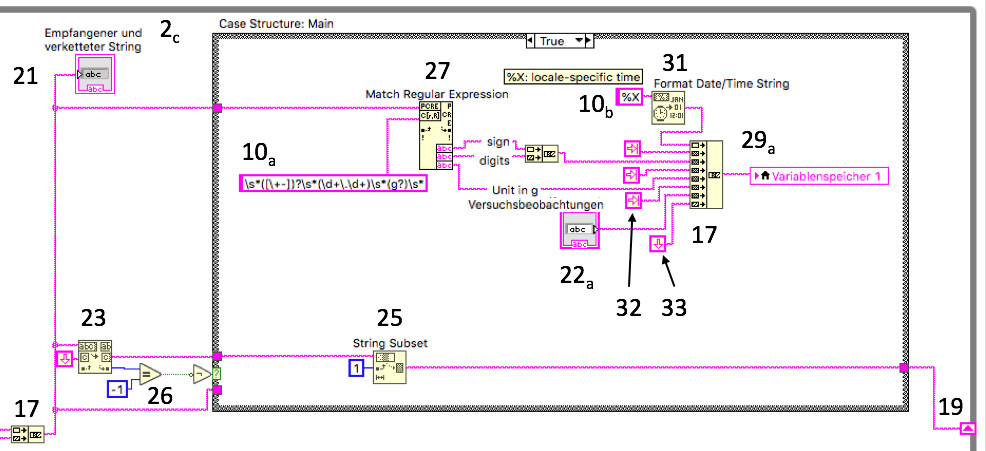
\includegraphics[width=1.05\textwidth]{Bilder/LabVIEW_serialport/stringkonstruktion.jpg}
	\vspace{2pt}
	\caption[String-/Zeilenkonstruktion]{String-/Zeilenkonstruktion}
	\label{fig:String-/Zeilenkonstruktion}
\end{figure}


\paragraph{Fünfter Schritt: Zeitstempelprogrammierung}  Der Zeitstempel (\textit{engl. Time\-stamp}) kann durch die folgenden zwei Methoden implementiert werden. Bei der ersten Methode wird mittels des Objekts \textit{Format Date/Time String} (siehe Abbildung \ref{fig:String-/Zeilenkonstruktion} (31) und (10b)) eine frei formatierbare Zeitreihe möglich (für genauere Infos schauen Sie bitte in \cite{zeitreihenformatierung}). \\

\noindent Um als Zeitstempel die verstrichene Zeit in ms zu bekommen, ist das Objekt wie in der Abbildung \ref{fig:vtp_elapsed_time} zu Programmieren (VTP Elapsed Time Sub VI) (44). Durch diese Methode ist es möglich bei Aktivierung dieses VI`s eine Startzeit zu ermitteln. Die Startzeit wird für den Header und für den Start des Datalogs, nach Betätigung der Start {\Menlo Datalogging in Tabgetrennt.txt} Datei, benötigt. Aus diesem Grund sind zwei Kopien dieses VI`s nötig!

%%=================================================================================

\input{Benötigte_LabVIEW_Konfigurationsfunktionen_Teil_2}

%%=================================================================================
 

\begin{figure}[!ht] %Methode 2   simple Elapsed Time in ms Sub VI (37)
     \subfloat[][\texttt{true}\label{fig:true}]
     {\includegraphics[width=0.5\textwidth]
       {Bilder/LabVIEW_serialport/step7_elapsed_true.jpg}
     }
     \hfill     
     \subfloat[][\texttt{false}\label{fig:false}]
     {\includegraphics[width=0.5\textwidth]
       {Bilder/LabVIEW_serialport/step7_elapsed_false.jpg}
     }
     \caption[]{Methode 2 \glqq VTP Elapsed Time in ms\grqq{} Sub VI (37)\\     	
  }
  \label{fig:vtp_elapsed_time}
   \end{figure}


\paragraph{Sechster Schritt: Versuchsbeobachtungen} Es ist eine Kommentarfunktion gewünscht. Das Kommentar soll eingegeben werden können und nach der Bestätigung der Eingabe mit\, \,{\Menlo Enter}, soll der Kommentar zum Zeitpunkt der\, \,{\Menlo Enter} betätigung dem jeweiligen Zeitstempel zugeordnet werden. Dafür ist die Einstellung gemäß Abschnitt \ref{sec:LabVIEW_Einstellungen} vorzunehmen. Ein \textit{\textbf{Control}} Objekt (22) kann als Variablenspeicher interpretiert werden. Nach der Übergabe eines Wertes an das \,{\Menlo Control} Objekt des Kommentar muss diese nach der Ausgabe wieder gewiped werden. Zum \glqq löschen\grqq{} der letzten Eingabe in \,{\Menlo Control} Objekten, ist diese mit einer leeren Stringkonstanten zu überschreiben (siehe Abbildung \ref{datalogger} ) 29a. Der Programmablauf wäre dann wie folgt:


\begin{itemize} % Versuchsbeobachtungsreset
\singlespacing
\item Versuchsbeobachtung wird eingegeben (22a)
\item \textit{Case Selektor} wird getriggert durch Programmstart oder wenn die Dauer für ein Messwertaufnahmeintervall verstrichen ist
\item sobald der Datalogger Case Selektor getriggert wird, schaltet die \,{\Menlo Case Structure} auf \,{\Menlo true}
\item Löschen der \textit{Control Versuchsbeobachtung} durch die lokale Variable (298) 
\end{itemize}


\paragraph{Siebter Schritt: Dataloggerprogrammierung}
\label{sec:Datalogger}

Die Messwerte sollen in eine \,{\Menlo Tabulator} getrennte *.txt geschrieben werden. Als nächstes ist ein Datalogger zu programmieren (siehe Abbildung \ref{datalogger}). Mit den Objekten 38 bis 42 kann ein Datalogger programmiert werden, der jede \,{\Menlo While Loop} Iteration die Daten in ein *.txt schreibt, die er in der jeweiligen Iteration übergeben bekommt. Während einer Iteration, kann er beliebig viele Zeilen in die *.txt Datei schreiben. Im \,{\Menlo true} Case wird der String aus \textit{Variablenspeicher 1} in die *.txt Datei geschrieben, die in 40b, vor Programmausführung zu benennen ist (\,{\Menlo test\_aller\_Funktionen\_Beispiel.txt}). Mit dem \,{\Menlo Elapsed Time} Objekt (35) kann ein \,{\Menlo Control} Objekt programmiert werden, mit dem das Wertaufnahmeintervall in s eingestellt werden kann. Diese wird mit der Funktion \,{\Menlo Time Target} (s)} des \,{\Menlo Elapsed Time} (43) Objekts verbunden. Über diese Control kann man das Messwertaufnahmeintervall varieren, auch während des Programmablaufs. Der \textit{Time has Elapsed} boolsche Ausgang ist mit einem \,{\Menlo Or} (46) zu verbinden \,{\Menlo Case Selector}. Wenn der Iterations Index 0 oder die angegebene Zeit verstrichen ist, wird ein Messwert gelogged, bzw. alle Zeile in die *.txt Datei geschrieben, die dem \textit{Write to Text File} (38) Objekt übergeben wird. Im \,{\Menlo false} Case soll nix passieren, daher werden die Tunnel (insgesamt 2 x 2) beider \,{\Menlo Case Structure} Seiten mit einander verbunden. Der \textit{Variablenspeicher 1} wird mit einem leeren String gelöscht (\textit{engl. wiped}, umgangsprachlich gewiped). Damit ist der \textit{Variablenspeicher 1} bis zur nächsten Eingabe geleert.

\bild{1.05}
{LabVIEW_serialport/step8_datalogger.jpg}
{-1em}
{Datalogger}
{Datalogger}
{datalogger}

\paragraph{Siebter Schritt ergänzung gemäß neuster Applikationen: Graph mit zwei Plots}


Anmerkung: Aus zeitlichen Gründen wird auf eine genaue Bezeichnung verzichtet. Die Initialisierung gemäß Abbildung \ref{datalogger} ist zu erweitern, damit der Datalog per Knopfdruck geschehen kann. Die \textit{case structure} hat eine {\Menlo and} Bedingung erhalten, damit das Datalogging per Knopfdruck getriggert wird (siehe Abbildung \ref{fig:datalogger_inie_true}). In Abbildung \ref{fig:datalogger_inie_true} und \ref{fig:datalogger_inie_false} ist das {\Menlo VTP\_ElapsedTime.vi} zu erkennen. Damit bekommt der Datalogger eine Startzeit. In der Abbildung \ref{fig:Graphfürzwei} ist die Erstellung des Graphen mit zu erkennen. Der Graph ist zum Plotten der Arrays {\Menlo Volumenstrommesswerte\_arr\_input} und {\Menlo Druckmesswerte\_arr\_input}. Die Arrays werden mit der Build Array Methode pro Iteration erweitert. Damit im Verlauf der Messung auch Zahlen im Blockdiagramm erkennbar sind wurde jeweils ein {\Menlo Array Indicator} dem Draht hinzugefügt und die Anzeige gespiegelt. Die Spiegel dient dazu, dass der neuste Wert oben im Array angezeigt wird. Der Graph bekommt seine Zeitreihenwerte vom {\Menlo VTP\_ElapsedTime2.vi} (siehe Abbildung \ref{fig:datalogger_inie_true}). Die Zeitreihen und Messwert Arrays werden mittels {\Menlo Cluster Bundle} zusammengeführt. Die erstellten {\Menlo Cluster} werden mittel der {\Menlo Build Array Methode} zusammengeführt und dem Graph als Dateninput geliefert. Das Graph VI kann aus einem Build XY Graph extrahiert werden (Doppelklick \> Strg +E etc.). Für den {\Menlo false case} werden alle Drähte mit dem zugehörigen {\Menlo shift register} verbunden.

\begin{figure}[p!] % 
% \captionsetup{position=top}
    \centering
        \subfloat[][Graph/Dataloggerinitialiserung true \label{fig:datalogger_inie_true}]{%
            \hspace{0em}
            \includegraphics[width=0.55\textwidth]
            {Bilder/LabVIEW_serialport/datalogger_links_neu.jpg} %{Bilder/LabVIEW_serialport/}
        }\hspace{0.05em}
        \subfloat[][Graph/Dataloggerinitialiserung false \label{fig:datalogger_inie_false}]{%
            \hspace{0em}
            \includegraphics[width=0.3\textwidth]
            {Bilder/LabVIEW_serialport/datalogger_links_neu_false.jpg} %{Bilder/LabVIEW_serialport/}
        }
    \phantomcaption
    \vspace{1em}
    \ContinuedFloat
%\captionsetup{position=bottom}
    \subfloat[][Graph für zwei kontinuierliche Parameter \label{fig:Graphfürzwei}]{%
        \includegraphics[width=0.9\textwidth]
        {Bilder/LabVIEW_serialport/datalogger_rechts_neu.jpg} %{Bilder/LabVIEW_serialport/}
    }
    \caption[Graph für zwei kontinuierliche Parameter]{Graph für zwei kontinuierliche Parameter}
    \label{}
\end{figure}



\paragraph{Achter Schritt: Diskrete Daten am Beispiel des Datalog Headers}

In der Abbildung \ref{fig:modularer_header} ist exemplarisch die erste Headerzeile (a) und die Methode (b), wie man diese mittels \textit{Concatenate} (17) verkettet abgebildet. Um eine schnelle und einfache Zusammenstellung der Headerkomponenten sowie die Übersichtlichkeit gewährleisten zu können, wird aus jedem Headereintrag ein Sub VI erstellt (siehe Abbildung \ref{fig:modularer_header} (b)). Der Datalogger Header ist somit einfach zu modifizieren.

%\newpage
%\begin{figure}[h] % Headerkonfiguration  standardheader Zeile und Zeitreihenheader
%     \subfloat[][Erste Header Zeile\label{fig:standard_header}]{%
%       \includegraphics[width=0.5\textwidth]
%       {Bilder/LabVIEW_serialport/standard_header.jpg}
%     }\hfill     
%    \subfloat[][Zeitreihen Überschrift\label{fig:header}]{%
%       \includegraphics[width=0.5\textwidth]
%      {Bilder/LabVIEW_serialport/header.jpg}
%     }\phantomcaption
%     %\caption[]{}
%%  \label{fig:simple_elapsed_time}
%   \end{figure}
%\begin{figure}[h] % Headerkonfiguration 2 Masse Dokumentenheader
%\ContinuedFloat
%\subfloat[][Masse Header Zeile\label{fig:vtp_masse}]{%
%       \includegraphics[width=0.5\textwidth]
%       {Bilder/LabVIEW_serialport/masse.jpg}
%     }\hfill     
%    \subfloat[][Verkettung der Headermodule\label{fig:dokumentenheader}]{%
%       \includegraphics[width=0.5\textwidth]
%      {Bilder/LabVIEW_serialport/Dokumentheaderverkettung.jpg}
%     }    
%\caption[Modulare Header Sub VI's]{Modulare Header Sub VI's}
%\label{fig:modularer_header}
%   \end{figure}

\begin{figure}[h] % Headerkonfiguration  standardheader Zeile und Zeitreihenheader
\centering
     \subfloat[][Erste Header Zeile\label{fig:standard_header}]{%
       \includegraphics[width=0.49\textwidth]
       {Bilder/LabVIEW_serialport/standard_header.jpg}
     }%\hfill     
    \subfloat[][Verkettung der Headermodule\label{fig:dokumentenheader}]{%
       \includegraphics[width=0.49\textwidth]
      {Bilder/LabVIEW_serialport/Dokumentheaderverkettung.jpg}
     }    
\caption[Modulare Header Sub VI's]{Modulare Header Sub VI's}
\label{fig:modularer_header}
   \end{figure}

\paragraph{Neunter Schritt: Auslastungsoptimierung} Um die optimale Taktrate für das Programm empirisch zu ermitteln, kann man eine \,{\Menlo LED} (30) zwischen den Objekten \,{\Menlo Equal?} (26) und \,{\Menlo Not} (27) platzieren. Nun variiert man die Taktrate  der \textit{While Loop} des  \textit{Haupt VI's}, bis die \,{\Menlo LED} für die Optimierung blinkt, um Daten \textit{Just in Time} zu erhalten. Mit dem Objekt \,{\Menlo wait (ms)} (34) kann man eine Wartedauer vor jeder Iteration einstellen. Mit dem Objekt \,{\Menlo wait until next ms multiple} (35) kann man eine Taktzeit für einen Iteration einprogrammieren. Die Dauer der Pause, bzw. die Taktrate jeder Iteration sollte geringer sein als die Dauer die benötigt wird, um die Daten von dem seriellen Port auszulesen. Das Blinken signalisiert, dass der (Read Buffer) der Datenquelle nicht überfüllt (engl. \textit{buffer overflow}) wird. Damit ist gewährleistet, dass für das Ausführen des Programms \textbf{ nur soviel Rechenkapazität verwendet wird wie nötig, jedoch genug, damit keine Daten verloren gehen oder eine Totzeit entsteht!} Um die Taktrate rechnerisch zu ermitteln, benötigt man die zu erwartenden \,{\Menlo Bytes}, bzw. character pro Zeile. Die Baudrate (Bd) gibt an, wie viele \textbf{Zeichen} pro Sekunde versendet werden. In vielen fällen wird für 1\,\textbf{Zeichen},
\,1\,\,{\Menlo Bit} benötigt, daraus folgt, dass die Baudrate in diesen Fällen \,{\Menlo Bit} pro s bedeutet.\\

Um ein 7 \,{\Menlo Bit} encodiertes \,{\Menlo Byte} zu versenden, werden 3 weitere \,{\Menlo Bit} auf der Datenleitung versendet. In der Tabelle \ref{tab:678bit} sind die Konfigurationsmöglichkeiten bei der Nutzung von 6, 7 oder 8 \,{\Menlo Bit} Encodierung und RS-232.

\begin{table}[hpt!] %6, 7, 8 Bit Encodierung via RS-232
\caption{\,{\Menlo 6}, \,{\Menlo 7}, \,{\Menlo 8} \,{\Menlo Bit}-{\Menlo Encodierung} via RS-232}
\begin{center}
\begin{tabular}{|r|c|c|c|}
\cline{2-4}
\multicolumn{1}{c|}{} &	\,{\Menlo 6} \,{\Menlo Bit} 		& \,{\Menlo 7} \,{\Menlo Bit} 		& \,{\Menlo 8} \,{\Menlo Bit}\\
\hline
 \,{\Menlo Startbit} 				& \,{\Menlo 1}				 & \,{\Menlo 1} 			& \,{\Menlo 1}\\ \hline
 \,{\Menlo Symbol-/Characterbit} & \,{\Menlo 6} 			& \,{\Menlo 7} 			& \,{\Menlo 8}\\ \hline
 \,{\Menlo Paritätsbit} & \multicolumn{2}{c|}{\hspace{3pt} {\Menlo Odd/Even/Mark/Space} \hspace{3pt}} & \,{\Menlo none}  \\ \hline
\,{\Menlo Stoppbit}	& 	\,{\Menlo 2} &	\,{\Menlo 1}& \,{\Menlo 0}\\ \hline
\,{\Menlo Baudrate in Bd} & \multicolumn{3}{c|}{\hspace{3pt} {\Hypatia diverse Möglichkeiten} \hspace{3pt}}   \\ \hline
 \,{\Menlo Handshake} & \multicolumn{3}{c|}{\hspace{3pt} \,{\Menlo Software/Hardware} \hspace{3pt}}  \\ \hline
\end{tabular}
\end{center}
\label{tab:678bit}
\end{table}

Die Dauer zum empfangen einer \textbf{Zeile} (\,{\Menlo '+'} oder \,{\Menlo '-'} + floatnumber + potentiells \,{\Menlo 'g'}), die 7 oder 8 \,{\Menlo bit} ASCII encodiert ist und via RS-232 Schnittsttelle versendet wird , lässt sich wie folgt berechnen (Annahmen: Bd = 1200 $\frac{\,{\Menlo Byte}}{\mathrm{s}}$, 15 $\frac{\,{\Menlo Byte}}{\mathrm{Zeile}}$, 10 $\frac{\,{\Menlo Bit}}{\,{\Menlo Byte}}70
$). 


% Sendegeschwindigkeit pro Zeile
\begin{align} 
1	\mathrm{Bd} 	&=	1	\,	\mathrm{Zeichen/		\texttt{Bit} \,	pro \, Sekunde} \\
1	\, \,	\texttt{Byte}	&=	10	\, \,	\texttt{Bit} \\
15 \, \,	 \texttt{Byte} &= 1 \, \mathrm{Zeile} \\
 \frac{1}{1200}  \frac{\mathrm{s}}{\texttt{Bit}} \cdot
  10 \,\, \frac{\texttt{Bit}}{\texttt{Byte}} \cdot
   15 \,\,  \frac{\texttt{Byte}}{\mathrm{Zeile}} 	&=
    0,125 \, \mathrm{s \, pro \, Zeile} \\
    											&\equiv 125 \, \mathrm{ms \, pro \, Zeile}
\end{align}


\subsubsection{NI DAQmx Programmierung am Beispiel der Wirbelschichtanlage}

Neben Geräten, die einen integrierten analog digital Wandler haben, gibt es Sensoren, die lediglich das analoge Signal transmittieren. Folglich muss das analoge Signal in ein digitales Signal umgewandelt werden. Für den Fall das Sensoren keinen integrierten analog/digital Wandler besitzen, ist eine Messkarte zwischen Sensor und PC zu implementieren (siehe Abbildung \ref{fig:sensor_analog_schnittstelle}). \\

\begin{figure}[b!] %[htbp!] 
\centering
\includegraphics[width=1\textwidth]{Bilder/sensor_analoge_schnittstelle.jpg}
\vspace{0em}
 \caption[DAQ von Messeinrichtungen mit analoger Schnittstelle]{DAQ von Messeinrichtungen mit analoger Schnittstelle}\label{fig:sensor_analog_schnittstelle}
\end{figure}



\begin{figure}[b!] % 
% \captionsetup{position=top}
    \centering
        \subfloat[Druck- und Volumenstromsensor Initialisierung der Wirbelschicht][Druck- und Volumenstromsensor Initialisierung der Wirbelschicht \label{fig:daq_ini}]{%
            \hspace{0em}
            \includegraphics[width=0.7\textwidth]
            {Bilder/Wirbelschicht_Appfotos/Wirbelschicht_datai_DAQ_ini.jpg} %{Bilder/LabVIEW_serialport/}
        }
    \phantomcaption
    \vspace{1.5em}
    \ContinuedFloat
%\captionsetup{position=bottom}
    \subfloat[DAQ read sub vi options][DAQ read options \label{fig:DAQ_read_option}]{%
        \includegraphics[width=0.7\textwidth]
        {Bilder/Wirbelschicht_Appfotos/Wirbelschicht_daq_read_option.jpg} %{Bilder/LabVIEW_serialport/}
    }
    \caption[DAQ Programmierung, Initialisierung und read.vi]{DAQ Programmierung, Initialisierung und read.vi}
    \label{fig:DAQ_Programmierung}
\end{figure}

Die NI Messkarte des Typs USB-6001 nennt sich in LabVIEW \textit{DAQmx}. Im folgenden Abschnitt wird die DAQ eines Volumenstromsensors und eines Druckssensors mittels USB-6001 Messkarte von National Instruments erläutert. In der Abbildung \ref{fig:daq_ini} ist die Initialisierungssequenz abgebildet, um analoge Signale von zwei Sensoren zu akquirieren. Es ist zu erkennen, das zwei Variablen (Zeitstempel,... ; Versuchsbeobachtungen), mittels lokaler Variable durch einem leeren String initialisiert werden.  Diese Form der Initialisierung hat eine Löschung der Werte aus der vorherigen Iteration zur Folge. Darunter ist die Initialisierung der DAQ Aufgabe (\textit{engl. task}), gefolgt von der Erstellung von zwei virtuellen Kanälen (\textit{engl. channel}) zu erkennen. Die Reihenfolge wurde zufällig gewählt. Es ist zu erkennen, dass der erste \,{\Menlo channel} den Drucksensor abfragt. Für den Drucksensor ist der Modus Operandi (Betriebsmodus) single ended ({\Menlo RSE}) auszuwählen. Die minimalen und maximalen Signal- bzw. Spannungswerte entsprechen 0~und~10~V. Der Drucksensors ist an Slot {\Menlo ai1} angeklemmt. Das DAQmx Gerät hat im System die Kennung {\Menlo Dev1} erhalten, daraus folgt das der Slot {\Menlo \,Dev1/ai1} auszuwählen ist. Für den Volumenstromsensor ist analog vorzugehen. Gemäß der elektrotechnischen Verschaltung (siehe Abbildung \ref{fig:wirbelelektrotechnik} im Abschnitt \ref{sec:schaltung}) ist das Signal des Volumenstromsensors nach dem Strom-/Spannugnswandler differenziel (double ended), daher ist als Modus \,{\Menlo Differentiall} auszuwählen.  Die Signalspanne ist analog des Drucksensors von 0~bis~10~V. Der Draht mit den Messignalen und der Errordraht betreten die While-Loop via \,{\Menlo Shift Register}. Das Auslesen wird mit dem {\Menlo DAQmx~Read.vi}, mit den Optionen gemäß \ref{fig:DAQ_read_option} durchgeführt.\\



An der Stelle muss die serielle Abfrage Programmiert werden. In der Abbildung \ref{fig:Druck_DAQ} ist zu erkennen, dass der \textit{\textbf{for loop} tunnel} (ist am \textcolor{blue}{{\Menlo N}} zu erkennen) ein weißer Kasten mit orangen Klammern ist. Das bedeutet, dass die \textbf{\textit{for loop}} betretenden Werte indexiert sind. Während \textbf{einer \textit{while loop} Iteration} erfolgen \textbf{zwei \textit{for loop} Iterationen}. Zur Erinnerung wird an dieser Stelle noch mal erwähnt, dass LabVIEW alles (Arrays, Schleifen etc.) mit dem Index null initiiert. Pro \textit{\textbf{while loop}} Iteration werden die Werte, die in die \textbf{\textit{for loop}} eintreten  also immer mit 0 und 1 indexiert. Der case structure selector muss mit dem \,{\Menlo equal?} Vergleichsoperator abfragen, ob der Wert 0 oder 1 ist. Das Signal des Drucksensors hat den Index 0, da es der erste channel ist, der initialisiert wird (vgl. Abbildung \ref{fig:daq_ini}). An dieser Stelle ist nun ein Gleichungssystem zu lösen. Der Sensor hat eine Messspanne von -1~bis~1~bar. Das elektrische Signal geht von 0~bis~10~V. Gemäß Abschnitt \ref{sec:quader} ist die Approximation durch eine Gerade hinreichend. Daraus folgt, dass für den Fall, dass die Spannung am DAQ Gleich 0 ist folgende Gleichung:

\begin{align}
p&=a \cdot x+b \\
-1~\mathrm{bar} &= a \cdot 0~\mathrm{V}+b \\
-1~\mathrm{bar} &=b \label{eq:druck_pt1}
\end{align}

Für den Fall, dass die Messkarte 10~$\mathrm{V}$ anzeigt gilt in Kombination mit Gleichung \ref{eq:druck_pt1}

\begin{align}
1~\mathrm{bar} &=a \cdot 10~\mathrm{V} -1~\mathrm{bar} \\[0.5em]
a &= \frac{1~\mathrm{bar}+1~\mathrm{bar}}{10~\mathrm{V}} \\[0.5em]
a &= \frac{2~\mathrm{bar}}{10~\mathrm{V}} \\[0.5em]
p &= 0,2~\frac{\mathrm{bar}} {\mathrm{V}}-1~bar
\end{align}

Da ein linearer Zusammenhang besteht und der Druck relativ zur Atmosphäre angegeben wir kann der offset durch die Addition des atmosphärischen Drucks $1~\mathrm{bar}$ eliminiert werden. Der Multiplikationsfaktor 0,2~$\frac{\mathrm{bar}}{\mathrm{V}}$ ist somit der gesuchte Wert für die Signalumrechnung.\\

In der Abbildung \ref{fig:analog-digitaldrucksensor} ist der Vergleich der Analog- und Digitaldruckmessung als Funktion des analog gemessenen Durchfluss zu erkennen. Des Weiteren wurde von beiden Messwertreihen eine lineare Approximationsfunktion erstellt. Der Drucksensor hat zum Zeitpunkt dieser Messung in der LabVIEW Applikation (als Konstante) \textbf{zwei} signifikante Stellen. Eine Wiederholung dieser Messung wird empfohlen, daher wird auf eine Anzeige der Approximationsfunktion zur Berechnung der Geraden verzichtet. In der LabVIEW Applikation ist für den Drucksensor die Anzahl der signifikanten Nachkommastellen auf \textbf{vier} korrigiert worden (siehe Abbildung \ref{fig:DAQ_Programmierung}).\\

\begin{figure}[h!] %[htbp!] 
\centering
\includegraphics[width=0.8\textwidth]{Bilder/analog-digitaldrucksensor.jpg}
\vspace{0em}
 \caption[Analog-, Digitaldruckmessung als Funktion der analogen Volumenstrommesswerte]
{Analog-, Digitaldruckmessung als Funktion der analogen Volumenstrommesswerte}\label{fig:analog-digitaldrucksensor}
\end{figure}

In einem thermischen Massendurchflusssensor ist eine Wheatstone`sche Brückenschaltung als elektrotechnische Komponente verbaut. Das elektrische Ausgangssignal des Sensors ist demnach ebenfalls linear. Für den Volumenstromsensor ist folglich analog vorzugehen. Der Parameter $a$ des Volumenstromsensor ist somit $5~\frac{\mathrm{l}/\mathrm{min}}{\mathrm{V}}$, mit $b=0~\frac{\mathrm{l}}{\mathrm{min}}$.\\

In der Abbildung \ref{fig:volumenstrom_messung} ist eine Volumenstrommessung, analog sowie digital, sowie der Betrag der absoluten Differenz beider Messwertreihen als Funktion der Manometerdruckdifferenz in mm abgebildet. Bei beiden Messwertreihen ist ein linearer Zusammenhang zu erkennen. In Folge dessen wurden lineare Approximationsfunktionen erstellt. Des Weiteren ist zu erkennen, dass beide Messwertreihen divergieren. Die größte Abweichung hat einen Betrag von 6,7~$\frac{\mathrm{l}}{\mathrm{min}}$ Da der \glqq Wahre\grqq{} Wert unbekannt ist wird keine relative Abweichung sowie Standardabweichung ermittelt.\\ 



\begin{figure}[h!] %[htbp!] 
\centering
\includegraphics[width=1\textwidth]{Bilder/Volumenstrommessungsverleich.jpg}
\vspace{0em}
 \caption[Analog-/Digitalvolumenstrommessung sowie absolute Abweichung in l/min, als Funktion der Manometerdifferenz in mm]
{Analog-/Digitalvolumenstrommessung sowie absolute Abweichung in l/min, als Funktion der Manometerdifferenz in mm}\label{fig:volumenstrom_messung}
\end{figure}

\begin{figure}[h!] % 
% \captionsetup{position=top}
    \centering    
    \subfloat[Druck DAQ][Druck DAQ \label{fig:Druck_DAQ}]{%
        \includegraphics[width=0.6\textwidth]
        {Bilder/Wirbelschicht_Appfotos/druck_daq.jpg} %{Bilder/LabVIEW_serialport/}
    }
     \hspace{0.06em}
         \subfloat[][Clear Task \label{fig:clear_task}]{%
            \hspace{0em}
            \includegraphics[width=0.206\textwidth]
            {Bilder/Wirbelschicht_Appfotos/daq_endsequenz.jpg} %{Bilder/LabVIEW_serialport/}
        }
    \phantomcaption
    \vspace{1em}
    \ContinuedFloat
%\captionsetup{position=bottom}
     \subfloat[Volumenstrom DAQ][Volumenstrom DAQ \label{fig:Volumenstrom_DAQ}]{%
            \hspace{0em}
            \includegraphics[width=0.6\textwidth]
            {Bilder/Wirbelschicht_Appfotos/Volumenstrom_daq.jpg} %{Bilder/LabVIEW_serialport/}
        }
       
    \caption[DAQ und interpretation beider kontinuierlichen Paramter, Druck und Volumenstrom]
    {DAQ und interpretation beider kontinuierlichen Paramter, Druck und Volumenstrom}
    \label{fig:daq_p_v}
\end{figure}



Bei der Beendigung des Programms musst der DAQmx task terminiert werden, dafür ist das {\Menlo DAQmx Clear Task.vi} außerhalb der \textit{while loop} zu platzieren und mit dem Signal sowie error {\Menlo schift \mbox{register}} zu verbinden  (siehe Abbildung \ref{fig:clear_task}).


\paragraph{Haupt Programm Dataloggerintialisierung am Beispiel der Filterkuchenversuchsanlage} 
Im Verlauf des Projekts ist der Wunsch geäußert worden, dass die generierten Protokolle unveränderlich (Schreibschutz) sein sollen. Der Dateidialog (siehe Abbildung \ref{fig:Dateidialog} im Anhang) wird vor der Schreibschutzabfrage platziert (siehe Abbildung \ref{fig:schreibschutz_dialog}) und, im Falle einer versuchten Öffnung einer Datei mit Schreibschutzes, in der \,{\Menlo case structure} \, (\textcolor{OliveGreen}{{\Menlo No Error}}) entfernt. Im \,\textcolor{red}{{\Menlo Error}} {\Menlo case} werden die Tunnel beider Seiten verbunden (siehe Abbildung \ref{fig:schreibschutz_dialog}). Auf weitere Erläuterungen wird im Rahmen dieser Arbeit verzichtet
\label{sec:Pfad}

\begin{figure}[h!] %[htbp!] 
\centering
\includegraphics[width=0.8\textwidth]{Bilder/LabVIEW_serialport/Haupt_VI_unten_links_3.jpg}
\vspace{0em}
 \caption[Dataloggerinitialiserung]
{Dataloggerinitialiserung}\label{fig:schreibschutz_dialog}
\end{figure}


\paragraph{Haupt Programm Dataloggerheader am Beispiel der Filterkuchenversuchsanlage} 

An der Abbildung \ref{fig:filterkuchenheader} lässt sich erahnen, dass die Erstellung diskreter Daten in LabVIEW eine tiefgreifende Verschachtlungen mittels eigens erstellter Sub VI`s benötigt. Auf eine Erläuterungen wird im Rahmen dieser Arbeit verzichtet. Es ist zu erkennen, dass der verkettete String aus der \,{\Menlo while loop} geführt wird. \\

Im Verlauf des Projekts wurde der Wunsch geäußert eine weitere Datei, mit sogenannten Tubidimeter Daten, generieren zu lassen. Analog des Headers ist eine verschachtelte Programmierung der Tubidimeter Eingaben erfolgt. Auf eine Erläuterungen wird im Rahmen dieser Arbeit verzichtet. Diese Daten werden während der Versuchsdurchführung, nach der Beendigung (\,{\Menlo Stop}-Button im Frontpanel siehe Abbildung \ref{fig:FilterkuchenVersuchseingaben}) eines Messungsdurchlaufs eingefügt. Es werden laut Praktikumsanweisung pro Versuchstag hintereinander drei Messungen durchgeführt. Das Schreiben, in die Datei mit den kontinuierlichen Daten und in die Datei mit den Tubidimeter Daten, muss sich an der Stelle unterscheiden. Für die Tubidimeterdatei muss die gesamte Datei Überschrieben werden und nicht wie im Fall der kontinuierlichen Datei am Ende angehängt. \,{\Menlo Set File Position.vi} erhält an dieser Stelle die Konstante \,{\Menlo start} (siehe Abbildung \ref{fig:schreibschutz_dialog}).

\begin{figure}[h!] %[htbp!] 
\centering
\includegraphics[width=0.9\textwidth]{Bilder/LabVIEW_serialport/Filterkuchenheader.jpg}
\vspace{0em}
 \caption[Filterkuchenheader]
{Filterkuchenheader}\label{fig:filterkuchenheader}
\end{figure}

\paragraph{Haupt Programm Endsequenz}

Wird das Hauptprogramm via \,{\Menlo Stop}-Button beendet, dann erfolgt die Endsequenz gemäß Abbildung \ref{fig:endsequenz}. Die Daten werden an dieser Stelle in die geöffnete bzw. erstellte Datei geschrieben, diese Datei geschlossen und mit einem Schreibschutz versehen.  

\begin{figure}[h!] %[htbp!] 
 \centering
 \includegraphics[width=0.6\textwidth]{Bilder/LabVIEW_serialport/endsequenz.jpg}
 \vspace{0em}
  \caption[Endsequenz des Hauptprogramms]
 {Endsequenz des Hauptprogramms}\label{fig:endsequenz}
 \end{figure} 
\pagebreak

\subsection{Verwendung beider Programme}
\label{sec:Haupt_VI_Nutzung}

Damit die Kommentarfunktion wie gewünscht funktioniert, ist vor der Verwendung des Programms in den LabVIEW Einstellungen unter Environment \,{\Menlo  End Text entry with Enter key} einzustellen (siehe Abbildung \ref{endtextentry}). Ist diese Option nicht eingestellt, muss nach jeder Betätigung der \,{\Menlo Enter}-Taste, die Eingabe ein weiteres mal mittels eines Mausklicks auf einen schwarzen Haken, der neben dem VI Ausführen Pfeil (oben links im Front Panel) erscheint, quittiert werden.

\bild{0.7}
{LabVIEW_serialport/endtextentry.png}
{0em}
{Einstellung \glqq End text entry with Enter key\grqq{}}
{Einstellung \glqq End text entry with Enter key\grqq{}}
{endtextentry}

Es wurde eine \,{\Menlo Tab Control} verwendet, um verschiedene Registerfenster zu generieren, siehe folgende Liste:

\begin{itemize} % Haupt VI Reiter
\singlespacing
\item Versuchseingaben
\item Während der Messung
\item Tubidimeter
\item \textcolor{black!50}{Konfiguration}
\item \textcolor{black!50}{Debugging}
\end{itemize}

Wie der Liste (\textcolor{black!50}{Markierung}) und der Abbildung \ref{fig:FilterkuchenVersuchseingaben} zu entnehmen ist, sind die Tabs \textcolor{black!50}{Konfiguration} und \textcolor{black!50}{Debugging} nicht sichtbar. Zum erreichen dieser Tabs ist das Frontpanel mit einem Passwort zu entsperren (z.B. durch die Betätigung von \,{\Menlo Strg+E}) und gemäß Abbildung \ref{fig:Filterkuchen_go_to_debugging} im Anhang fortzufahren. \\

In der Abbildung \ref{fig:FilterkuchenVersuchseingaben} ist das Frontpanel für den Filterkuchenversuchstand abgebildet. Oben links im Bild ist das Programmstarticon $\Rightarrow$ zu erkennen. Für den Wirbelschichtversuchsstand sieht das Frontpanel identisch aus.\\

\begin{figure}[h!] %[htbp!] 
\centering
\includegraphics[width=0.8\textwidth]{Bilder/Filterkuchen_Appfotos/FK_Versuchseingaben.jpg}
\vspace{0em}
 \caption[Filterkuchen Frontpanel: Versuchseingaben]
{Filterkuchen Frontpanel: Versuchseingaben}\label{fig:FilterkuchenVersuchseingaben}
\end{figure}

Die Frontpanel Tabs für die kontinuierlichen Messungen sehen für beide Versuchsstände identisch aus (siehe Abbildung  \ref{fig:messung}). Unter dem Plotter ist links ein Eingabefeld für Versuchsbeobachten zu erkennen. Die Eingaben werden dem Zeitstempel, zum Zeitpunkt der \,{\Menlo Enter}betätigung, angehängt. Rechts von dem Eingabefeld für die Versuchsbeobachtungen sind die Arrays abgebildet, die oben den aktuellsten Messwert anzeigen. Das Schreiben der kontinuierlichen Daten (in einen String) erfolgt erst nach Betätigung des Buttons \,{\Menlo Start Datalogging in Tabgetrennt.txt Datei}. Die Endsequenz, in der die Daten der kontinuierlichen Messung sowie die der Tubidimetereingaben (siehe Abbildung \ref{fig:tubidimetereingaben}), in die geöffnete oder generierten Datei geschrieben werden, erfolgt nach dem Betätigen des \,{\Menlo Stop}-Buttons (siehe Abbildung \ref{fig:FilterkuchenVersuchseingaben}). 

\begin{figure}[h!] %[htbp!] 
\centering
\includegraphics[width=1\textwidth]{Bilder/Filterkuchen_Appfotos/Filterkuchen_diagramm.jpg}
\vspace{0em}
 \caption[Filterkuchen Frontpanel: Tab der kontinuierlichen Messung am Beispiel der Filterkuchenapplikation]
{Tab der kontinuierlichen Messung am Beispiel der Filterkuchenapplikation}\label{fig:messung}
\end{figure}

\begin{figure}[h!] %[htbp!] 
\centering
\includegraphics[width=1.07\textwidth]{Bilder/Filterkuchen_Appfotos/Tubidimeter_FP_Eingaben.jpg}
\vspace{0em}
 \caption[Filterkuchen Frontpanel: Tab der Tubidimetereingaben]
{Filterkuchen Frontpanel: Tab der Tubidimetereingaben}\label{fig:tubidimetereingaben}
\end{figure}



In der Abbildung \ref{fig:funktionstest} ist ein Datalog eines Wirbelschichtestdurchlaufs zu erkennen. Diese \,{\Menlo .txt} Datei wurde in Excel Importiert. Es ist zu erkennen, dass diese Messwerte vier signifikante Stellen aufweisen. Es kann vorkommen, dass die automatische Datenimportfunktion das Spaltentrennzeichen nicht erkennt, dann ist gemäß Micosofts Problembehungshinweis fortzufahren (siehe Teilausschnitt in Abbildung \ref{fig:legacy}). Im Falle der Tubidimeterdatei ist dies der Fall gewesen, daher wird der Import nicht automatisch eingefärbt (siehe Abbildung \ref{fig:tubidimeter_import}). Des Weiteren ist zu erkennen, dass die Eingaben keine Restriktionen enthalten (int8, 16, 32, 64; float8, ...; die Ziffer steht für die Bytelänge). Alle Eingaben sind \,{\Menlo Strings}, dass bedeutet, es ist im Textformat. Bei der Weiterverarbeitung ist eine Umwandlung in ein int oder float zu erfolgen (in Excel\,{\Menlo  Zelle formatieren..}).


\begin{figure}[h!] % 
% \captionsetup{position=top}
    \centering
      \vspace{-1em}
        \subfloat[Datalogimport der kontinuierlichen Daten in Excel, am Beispiel der Wirbelschicht Daten]
        [Datalogimport der kontinuierlichen Daten in Excel, am Beispiel der Wirbelschicht Daten \label{fig:funktionstest}]{%
            \hspace{0em}
            \includegraphics[width=0.7\textwidth]
            {Bilder/Wirbelschicht_Appfotos/Wirbelschicht_Versuchseingaben_datalog_klein.jpg} %{Bilder/LabVIEW_serialport/}
        }
    \phantomcaption
    \vspace{0.7em}
    \ContinuedFloat
%\captionsetup{position=bottom}
    \subfloat[Legacy Import, gemäß Microsoft][Legacy Import, gemäß Microsoft \label{fig:legacy}]{%
        \includegraphics[width=0.7\textwidth]
        {Bilder/ms_legacy.jpg} %{Bilder/LabVIEW_serialport/}
    }
     \phantomcaption
    \vspace{0.7em}
    \ContinuedFloat
%\captionsetup{position=bottom}
    \subfloat[Tubidimeter Datalogimport in Excel][Tubidimeter Datalogimport in Excel \label{fig:tubidimeter_import}]{%
        \includegraphics[width=0.7\textwidth]
        {Bilder/Filterkuchen_Appfotos/tubidimeter.jpg} %{Bilder/LabVIEW_serialport/}
    }
    \caption[Datalogs und Excel troubleshooting]{Datalogs und Excel troubleshooting}
    \label{}
\end{figure}


%\begin{figure}[h!] %[htbp!] 
%\centering
%\includegraphics[width=0.7\textwidth]{Bilder/Wirbelschicht_Appfotos/Wirbelschicht_Versuchseingaben_datalog_klein.jpg}
%\vspace{0em}
% \caption[Datalogimport der kontinuierlichen Daten in Excel, am Beispiel der Wirbelschicht Daten]
%{Datalogimport der kontinuierlichen Daten in Excel, am Beispiel der Wirbelschicht Daten}\label{fig:funktionstest}
%\end{figure}

%\begin{figure}[h!] %[htbp!] 
%\centering
%\includegraphics[width=0.8\textwidth]{Bilder/ms_legacy.jpg}
%\vspace{0em}
% \caption[Legacy Import, gemäß Microsoft]
%{Legacy Import, gemäß\cite{Windows2021}}\label{fig:legacy}
%\end{figure}

%\begin{figure}[h!] %[htbp!] 
%\centering
%\includegraphics[width=0.6\textwidth]{Bilder/Filterkuchen_Appfotos/tubidimeter.jpg}
%\vspace{0em}
% \caption[Tubidimeter Datalogimport in Excel]
%{Tubidimeter Datalogimport in Excel}\label{fig:tubidimeter_import}
%\end{figure}



\FloatBarrier

\subsubsection{Fazit}

Die implementation eines Cloudservice (HAW Cloud) ist im Verlauf des Projekts nicht erfolgt. Die HAW Richtlinien scheinen es \textbf{derzeit} nicht zu gestatten, dass Kennungen an nicht humane Entitäten bzw. nicht natürliche Personen vergeben werden. Nicht humane Entitäten könnten die folgenden sein:
 
\begin{itemize}
\item Geräte
\begin{itemize}
\item HMI's 
\item Sensoren
\end{itemize} 
\item Aggregate
\item Maschinen
\end{itemize}

Die Idee, dass jeder Laboraccount eine eigene Kennung erhält, wodurch die Laborgeräte wie HMI's ein Cloudverzeichnis auf der HAW Cloud erhalten würden, ist derzeit nicht realisierbar. Die Idee, dass nicht humane Entitäten eine Kennung erhalten können, sollte in höheren Instanzen der HAW diskutiert werden, damit zukünftige Cloudlösungen HAW global realisiert werden können. Die Hochschule sollte das Ziel haben die Privatwirtschaft abzubilden. Das nicht humane Entitäten ein eigenes Kommunikationbsnetzwerk erhalten ist bereits Stand der Technik (siehe Abschnitt \ref{sec:bluetooth}). \\

Es ist anzumerken, dass die \,{\Menlo Controls} für die diskreten Eingaben keine Eingaberestriktionen besitzen und alles im Textformat gespeichert wird.

\pagebreak
\section{Praktische Teilumsetzung des Konzepts 3.0 an ausgewählten Versuchsständen}

Gemäß der Aufgabenstellung wurde zu Beginn des Projekts eine Analyse durchgeführt, um herauszufinden wie viele Versuchsstände digitale Schnittstellen besitzen. In Folge dessen wurde der \textit{Grad der Digitalisierung} definiert (Schnittstellen vorhanden, \glqq effektive\grqq{} Schnittstelle; gemäß Tabelle \ref{tab:grad_der_digitalisierung}) und ermittelt, wie hoch der prozentuale Anteil der MVT Versuchsstände ist, bei denen bereits Daten akquiriert werden können. Unter anderem war ein Ergebnis der Analyse, dass zwei Versuchsstände (Wirbelschicht und Filterkuchen), mit digitaler Messtechnik bzw. Sensoren aufgerüstet werden sollen. In den folgenden Abschnitten wird die praktische Modifikation der Versuchsstände erläutert.\\

\subsection{Filterkuchenversuchsanlage}

Im Rahmen dieser Arbeit wurde die Filterkuchenversuchsanlage (siehe Abbildung \ref{fig:filterkuchenversuchsstand})  aufgerüstet. Das Fließschema der Anlage zu Projektbeginn ist der Abbildung \ref{fig:schema_filterkuchenversuchsstand}
zu entnehmen. Bei diesem Versuchsstand gibt es zwei Absperrhähne. Der erste Absperrhahn ({\Hypatia H1}) verriegelt das Leitungssystem gegen die Vacuumpumpe ({\Hypatia A}), somit kann ein Unterdruck während Versuchsvorbereitungen oder umbauten aufgebaut werden. Das Manometer ({\Hypatia B}) ist in der Vacuumpumpe integriert. Der zweite Absperrhahn ({\Hypatia H2}) verriegelt den Trübebehälter ({\Hypatia J}), indem ein Rührer ({\Hypatia K}) das Aussedimentieren der Suspension unterbindet. Unter dem Trübebehälterbefinden sich Kuststoffklemmen ({\Hypatia G}) und Gummiringe , um die Filternutschen ({\Hypatia I}) zu fixieren und abzudichten. Die Filternutschen werden mit dem Filtratauffangbehälter ({\Hypatia D}) verbunden, welcher sich bei Versuchsstillstand auf einer Schutzplatte ({\Hypatia E}) befindet, um die Digitalwaage ({\Hypatia F}) vor einer Dauerlast zu bewahren. Des Weiteren schützt die Schutzplatte die Waage bei Versuchsumbauten. Vor dem Starten eines Versuchsdurchlaufs ist die Schutzplatte ({\Hypatia E}) zu entfernen und der Filtratauffangbehälter ({\Hypatia D}) auf der Waage zu positionieren. Zwischen der Vacuumpumpe (Richtung {\Hypatia A}) und dem Filtratauffangbehälter ({\Hypatia D}) befindet sich ein Pufferbehälter, um dem Pufferbehälter vor einer potentiellen Suspensionskontamination zu bewahren. Die Filterkuchenversuchsanlage wird im Rahmen der Präsenzveranstaltungen isobar betrieben. Die Gleichungen zur Berechnung der Filtrationsanlage sind dem Abschnitt \ref{sec:darcygleichung} zu entnehmen. Die linearisierte Filtrationsgleichung, auf der Grundlage der Darcy-Gleichung, ist nachfolgend aufgeführt:

\begin{equation}
\label{eq:irr_alpha_beta_kappa_integration_linearisiert_dpdt_2}
\frac{t}{V(t)} = \underbrace{\frac{\eta \cdot\alpha_\mathrm{V} \cdot \kappa}{A^2 \cdot 2 \cdot \Delta p_{\mathrm{konst,irr}}}
\cdot V(t)}_{\substack{a_1}}  +  \underbrace{\frac{\eta \cdot \beta}{A \cdot \Delta p_{\mathrm{konst,irr}}}}_{\substack{a_0}}
\end{equation}

Die zu bestimmenden Parameter sind der folgenden Auflistung zu entnehmen:

\begin{figure}[b!] % 
% \captionsetup{position=top}
    \centering
        \subfloat[][Filterkuchenversuchsstand vor den Modifikationen\label{fig:filterkuchenversuchsstand}]{%
            \hspace{0em}
            \includegraphics[width=1\textwidth]
            {Bilder/filterkuchversuchsstand.jpg} %{Bilder/LabVIEW_serialport/}
        }
    \phantomcaption
    \vspace{1em}
    \ContinuedFloat
%\captionsetup{position=bottom}
    \subfloat[Fließschema in Form einer schematischen Skizze der Filterkuchenversuchsanlage vor den Modifikationen]
    [Fließschema in Form einer schematischen Skizze der Filterkuchenversuchsanlage vor den Modifikationen \cite{Kuchenfiltration_Geweke2020} \label{fig:schema_filterkuchenversuchsstand}]{%
        \includegraphics[width=0.75\textwidth]
        {Bilder/filterkuchversuch_schema.jpg} %{Bilder/LabVIEW_serialport/}
    }
    \caption[Filterkuchenversuchsanlage nach den Modifikationen]{Filterkuchenversuchsanlage nach den Modifikationen}
    \label{}
\end{figure}



\begin{enumerate}[label = \textbullet, itemsep = -.1em]
\item \textbf{diskret}
	\begin{enumerate}[label = --, itemsep = -.1em]
	\item a0
			\begin{enumerate}[label = -, itemsep = -.1em]
			\item die Viskosität $\eta$
			\item der Filtermittelwiderstand $\beta$
			\item die Filtrationsfläche $A$
			\end{enumerate}
	\item a1
		\begin{enumerate}[label = -, itemsep = -.1em]
		\item der Filterkuchenwiderstand $\alpha_\mathrm{V}$
		\item die Proportionalitätskonstante $\kappa$
		\item die Filtrationsfläche $A$
		\item die Viskosität $\eta$
		\end{enumerate}
	\item die Fluiddichte $\rho_\mathrm{f}$
	\item die Feststoffdichte $\rho_\mathrm{fs}$
	\end{enumerate}
	
\item \textbf{kontinuierlich}
	\begin{enumerate}[label = --, itemsep = -.1em]
	\item der irreversible Druckverlust $\Delta p_{\mathrm{konst,irr}}$
	\item das Volumen als Funktion der Zeit $V(t)=$\,\text{\Large{$\frac{m_{\mathrm{Filtrat}}(t)}{{\Large \rho_\mathrm{f}}}$}}
	\end{enumerate}

\end{enumerate}

Das Filtrationsvolumen, als Funktion der Zeit, wird über die zusammengesetzte, extensive Zustandsgröße -- der Filtratmasse $m_{\mathrm{Filtrat}}(t)$ -- bestimmt. 

\subsubsection{Sensorauswahl}

  

Im Betrieb der Filterkuchenversuchsanlage sind die Parameter, Volumenstrom $\dot{V}$ und Druck $p$, kontinuierlich zu erfassen. Die Masse des Filtrats wird von einer Laborwaage des Unternehmens Sartorius AG des Typs Practum 5101-1S detektiert. Die Waage hat eine USB Schnittstelle, die mit einem USB Kabel eine RS-232 Schnittstelle emuliert. Dafür sind, gemäß der Bedienungsanweisung der Waage, die Einstellung mit den gewünschten Schnittstellenparametern vorzunehmen. Im Rahmen dieser Arbeit werden die Schnittstellenparameter gewählt, die in der Tabelle \ref{tab:678bit_2} \textbf{schwarz} hinterlegt sind. Die Auswahl der Parameter erfolgt willkürlich. Die Übertragungsgeschwindigkeit ({\Menlo 1200 Bd}) wurde hinreichend niedrig gewählt.\\

Es haben sich zwei Drucksensortechnologien etabliert, der dehnungsresistive Drucksensor und der piezeresistive Drucksensor. Im Anhang ist eine Vergleichstabelle (siehe Tabelle \ref{fig:metall_halbleiter_dms}), die beide Sensortypen verschiedener Hersteller und deren Spezifikationen auflistet. Gemäß der Tabelle ist zu entnehmen, dass piezoresistive Sensoren kleinere Dehnungen genauer Druckdifferenzen erfassen können. Die zu erwartenden Druckdifferenzen am Versuchsstand sind gering, daher wird ein piezoresistiver Relativdrucksensor des Unternehmens B+B Thermo-Technik GmbH des Typs DRTR-AL-10V-RV1 gewählt. Der Sensor ist im verfahrenstechnischem Labor ein häufig genutztes Messinstrument und ist im Verlauf dieser Arbeit bereits vorrätig gewesen, daher findet ein finanzieller Aufwandsvergleich im Rahmen dieser Arbeit nicht statt. Die Messspanne dieses Sensors ist von -1~bis~1~bar. Die Spanne des analogen Ausgangssignals ist von 0~bis~10~V. Die technischen Daten sind der Tabelle \ref{fig:BTTG2021} im Anhang zu entnehmen. \\

\begin{table}[hpt!] %6, 7, 8 Bit Encodierung via RS-232
\caption{RS-232 Schnittstellenparameter der Practum 5101-1S Waage}
\begin{center}
\begin{tabular}{|r|c|c|c|}
\cline{2-4}
\multicolumn{1}{c|}{} &	\textcolor{black!50}{6 {\Menlo Bit}} 		&  {\Menlo 7 Bit} 		&\textcolor{black!50}{ 8 {\Menlo Bit}}\\
\hline
{\Menlo Startbit} 				& \textcolor{black!50}{1}				 & {\Menlo 1} 			& \textcolor{black!50}{1}\\ \hline
{\Menlo Symbol-/Characterbit} & \textcolor{black!50}{6} 			& {\Menlo 7} 			& \textcolor{black!50}{8}\\ \hline
{\Menlo Paritätsbit} & \multicolumn{2}{c|}{\hspace{3pt}  {\Hypatia Odd}\textcolor{black!50}{/Even/Mark/Space} \hspace{3pt}} & \textcolor{black!50}{none}  \\ \hline
{\Menlo Stoppbit}	& \textcolor{black!50}{	2} &	{\Menlo 1}& \textcolor{black!50}{0}\\
\hline
{\Menlo Baudrate} &  \multicolumn{3}{c|}{\hspace{3pt}  \,{\Menlo 1200} \hspace{3pt}}    \\ \hline
\end{tabular}
\end{center}
\label{tab:678bit_2}
\end{table}


\pagebreak
\subsubsection{Elektrotechnik der Filterkuchenversuchsanlage}

Die Sensorik ist elektrotechnisch zu verschalten, die genutzten Komponenten sind: 

\begin{itemize}
\item als Spannungsquelle ein Transformator des Typs Voltcraft TOPS-3205   
\begin{itemize}
\item Conrad Electronic AG
\end{itemize}

\item ein Drucksensor des Typs DRTR-AL-10V-RV1
\begin{itemize}
\item B+B Thermo-Technik GmbH
\end{itemize}


\item eine Laborwaage des Typs Practum 5101-1S
\begin{itemize}
\item Unternehmens Sartorius AG 
\end{itemize}

\item eine DAQ Messkarte (\textit{engl. data acquisition}) des Typs USB-6001 
\begin{itemize}
\item National Instruments (NI)
\end{itemize}
\end{itemize}



\begin{figure}[h!] %[htbp!] 
\centering
\vspace{-3em}
\includegraphics[width=1.02\textwidth]{Bilder/Filterkuchen_Messtechnik.pdf}
\vspace{-4em}
 \caption[]{Elektrotechnische Verschaltung der Komponenten der Filterkuchenversuchsanlage}\label{fig:filterkuchenelektrotechnik}
\end{figure}


Die Elektrotechnische Verschaltung des Drucksensors ist der Abbildung \ref{fig:filterkuchenelektrotechnik} zu entnehmen. Die Laborwaage des Typs Practum 5101-1S wird, via mitgelieferten USB-Y zu RS-232 Schnittstellenemulationsprozessorstecker Kabel, mit dem Desktop PC verbunden. 

\subsubsection{Filterkuchenversuchsanlage nach den Modifikationen}

In der Abbildung \ref{fig:filterkuchenversuchsstand_upgrade} ist die gesamte Filterkuchenversuchsanlage, nach dem Aufrüsten mit digitaler Sensorik zu erkennen. Die Grafik des Schlauchleitungs- und Gerätefließschemas ist der Abbildung  \ref{fig:schema_filterkuchenversuchsstand_upgrade} zu entnehmen. Der Versuchsaufbau wurde um eine Spannungsquelle ({\Hypatia N}) für den Drucksensor ({\Hypatia M}), einen Drucksensor ({\Hypatia M}), sowie ein Human-Machine-Interface (HMI, {\Hypatia O}) erweitert. Als HMI dient ein Desktop PC. Das Manometer zur Druckmessung bildet mit der Vacuumpumpe ({\Hypatia B}) eine Einheit. 

\subsubsection{Workflow der Filterkuchenversuchsanlagen}

In diesem Abschnitt wird der neue Workflow beschrieben. Die Datalogs werden derzeit in dem Datalogordner auf dem Desktop gespeichert. Der Tabelle \ref{tab:filterkuchenversuchsanlagenbezeichnungen} sind die Bezeichnungen der Komponenten zu entnehmen.

\begin{enumerate}
\item \textbf{{\Hypatia Starten des HMI}}
	\begin{itemize}
		\item Inbetriebnahme der Spannungsquelle
			\begin{enumerate}[label = \roman*]
			\item Hauptschalter auf der Rückseite betätigen
			\item Spannungshöhe zwischen 15 und 24 V einstellen
			\item On-button auf der Vorderseite betätigen $\Rightarrow$ Spannung stellt sich auf den gewählen Betrag ein
			\end{enumerate}	
	\item Waagensignalleitung ist mit der RS-232 Schnittstelle des HMI Towers zu verbinden.
	\item DAQ ist mit einem beliebigen USB Slot des HMI Towers zu verbinden
	\item Starten der LabVIEW Applikation \: {\Menlo Filterkuchenversuch\_V01DL.vi}
	\item Dateinamen eingeben: FK\_{\Menlo GruppenID.txt}
		\begin{enumerate}[label = -]
		\item Der Dateiname kann über den Versuchstag identisch bleiben, die Daten werden an das Datei\-ende angehängt.
		\end{enumerate}
	\item Tubidimeterdateinamen eingeben: FK\_Tubi\_{\Menlo GruppenID.txt}
		\begin{enumerate}[label = -]
		\item Der Dateiname kann über den Versuchstag identisch bleiben, die Daten werden pro Versuchsiteration überschrieben.
		\end{enumerate}
	\item Versuchseingaben tätigen
	\item wenn alle Vorbereitung der Filtrationseinrichtung \textbf{abgeschlossen} sind, dann
		\begin{enumerate}[label = \Roman*]
		\item Start des Programms: Das $\Rightarrow$ Icon oben links 
		\item öffnen des Absperrhahns H2
		\item wenn Messung abgeschlossen, dann
			\begin{enumerate}[label = --]
			\item Stop betätigen
				\begin{enumerate}[label = -]
				\item Filtratmenge bestimmen 
				\item Filterkuchendicke bestimmen 
				\item die trockene Filterkuchenmasse bestimmen
				\end{enumerate}
			\item Tubidimeter eingaben tätigen
			\item wenn abgeschlossen,  starten der nächsten Iteration bei I		 
			 \end{enumerate}
			\item \textbf{Nach der letzten Tubidimetereingabe ist das Programm nochmals zu starten und der Stop-button zu betätigen, damit die aktuellsten Tubidimeterdaten in der \newline FK\_Tubi\_{\Menlo GruppenID.txt} gespeichert werden!} 
		\end{enumerate}	
	\end{itemize}


\item \textbf{{\Hypatia Vorbereitung der Filtrationseinrichtung}}
	\begin{enumerate}[label = \alph*]
	\item Absperrhahn H1 schließen
	\item Filtrationsanlage evakuieren, dazu ist die \textit{manuell} Taste des Vakuumcontrollers zu betätigen. Bei erreichen des Solldrucks wird der isobare Zustand der Anlage erhalten.
 	\item Gereinigte Filternutsche ({\Hypatia I}) in der Kunststoffklemmvorrichtung ({\Hypatia G}) fixieren.
 	\item Es ist darauf zu achten, dass der Metallsteg der Nutschenhalterung nach vorn zeigt
	\item Absperrhahn H2 schließen (Hebelstellung: waagerecht).
	\item Schläuche sachgemäß montieren.
	\item Schutzplatte der Waage entfernen und daraufhin einschalten.	
	\item Einfüllen der Suspension und Inbetriebnahme des Rührers. 
	\item Öffnen des Dreiwegehahns H1
	\item Wenn alle Vorbereitungen abgeschlossen sind und die angezeigte Masse Konstant ist, ist die Waage zu tarieren.
	 \end{enumerate}	
\end{enumerate}

 

\begin{figure}[p!] % 
% \captionsetup{position=top}
    \centering
        \subfloat[][Filterkuchenversuchsanlage nach den Modifikationen \label{fig:filterkuchenversuchsstand_upgrade}]{%
            \hspace{0em}
            \includegraphics[width=1\textwidth]
            {Bilder/HAW/filterkuchenversuchsanlage_upgrade.jpg} %{Bilder/LabVIEW_serialport/}
        }
    \phantomcaption
    \vspace{1em}
    \ContinuedFloat
%\captionsetup{position=bottom}
    \subfloat[Fließschema in Form einer schematischen Skizze der Filterkuchenversuchsanlage nach den Modifikationen][Fließschema in Form einer schematischen Skizze der Filterkuchenversuchsanlage nach den Modifikationen \cite{Kuchenfiltration_Geweke2020} \label{fig:schema_filterkuchenversuchsstand_upgrade}]{%
        \includegraphics[width=0.65\textwidth]
        {Bilder/filterkuchversuch_schema_upgrade.jpg} %{Bilder/LabVIEW_serialport/}
    }
    \caption[]{Filterkuchenversuchsanlage nach dem Aufrüsten mit digitaler Sensorik }
    \label{fig:Filterkuchenversuchsanlage_bezeichnet_upgrade}
\end{figure}

\begin{table}[h!]
\centering
\caption{Bezeichnungen der Filterkuchenversuchsanlage}\label{tab:filterkuchenversuchsanlagenbezeichnungen}
\vspace{0.5em}
{\Hypatia \begin{tabular}{r l r l}
A & Verbindung zur Vacuumpumpe 				&  H2	& Absperrhahn	\\[0.1em]
B 	& Vacuummanometer 								& I	& Filternutsche 		\\[0.1em]  
C & Rezipient und Wasserabscheider \quad \quad	& J & Trübebehälter  \\[0.1em]
D	& Filtratauffangbehälter    							& K 	& Rührer 				\\[0.1em]	
E & Schutzplatte für Waage 							&  L & Pufferbehälter		\\[0.1em]
F 	& Waage mit digitaler Schnittstlelle 				& M & Drucksensor 		\\[0.1em]	
G & Kunststoffklemmvorrichtung									& N & Spannungsquelle \\[0.1em]	
 & --~\,Gummidichtung 									& O & HMI (Human-Machine-Interface)\\[0.1em]	
H1 &  	Dreiwegehahn									& 		& \\ 
\end{tabular}}
\end{table}



\newpage
\subsection{Wirbelschichtversuchsanlage}

Das verfahrenstechnische Labor der HAW-Hamburg Life Sciences besitzt eine Wirbelschichtversuchsanlage im Labormaßstab (siehe Abbildung \ref{fig:Wirbelschicht_mod0}). In der Abbildung \ref{fig:Wirbelschicht_konzept} ist eine Versuchsskizze des Versuchsstands dargestellt. Der gesamten Anlage ist ein Druckminderer vorgeschaltet ({\Hypatia A}). Um den Volumenstrom zu Steuern, befindet sich nach dem Druckminderer ein Handventil ({\Hypatia B}). Zur Detektion des Volumenstroms sind zwei Schwebekörperdurchflussmesser (SKDM) ({\Hypatia C}) in reihe nachgeschaltet, um einen Volumenstrom von bis zu 50~l/min Messen zu können. Mit dem SKDM auf der rechten Seite kann der Messbereich von von 0,185~bis~5~l/min gemessen werden. Mit dem SKDM auf der linken Seite sind Volumenströme 1,86~bis~50~l/min messbar. Vor dem Anströmboden muss ein Druck gemessen werden, dafür befindet sich am Boden des Fluidisierapparats ({\Hypatia E}) ein kleiner Flansch, mit dem der Druck relativ zur Umgebung mittels U-Rohr Manometer ({\Hypatia D}) gemessen werden kann. Der Fluidisierapparat besteht aus einer Plexiglassäule und dem Boden, in dem ein Gewebefilter eingespannt ist. Da Partikel mit dem Volumenstrom ausgetragen werden können, befindet sich über dem Fluidisierapparat eine Absaugung ({\Hypatia F}).

Bei diesem Versuch sind im Verlauf der Versuchsdurchführung die folgenden Parameter zu erfassen:

\begin{enumerate}[label = \textbullet, itemsep = -.1em]
\item \textbf{diskret}
	\begin{enumerate}[label = --, itemsep = -.1em]
		\item Festbettbetthöhe $h_{\mathrm{fb}}$
		\item Festbettporösität $\varepsilon_{\mathrm{fb}}$
		\item Schüttgutmasse $m_{\mathrm{Schüttgut}}$
		\item Partikeldichte $\rho_{\mathrm{fs}}$
		\item Sauterdurchmesser
	\end{enumerate}  	
	
\item \textbf{kontinuierlich}
	\begin{enumerate}[label = --, itemsep = -.1em]
		\item $\dot{V}_{\mathrm{Luft}}$ 
		\item $\Delta p (t)$ 
	\end{enumerate} 
	
\item \textbf{kontinuierlich/diskret}
	\begin{enumerate}[label = --, itemsep = -.1em]
		\item Wirbelschichthöhe $h_{\mathrm{ws}} = f(p)$
		\item Wirbelschichtporösität $\varepsilon_{\mathrm{ws}}= f(p)$ 
	\end{enumerate} 
	
\end{enumerate} 

\begin{figure}[p!] % Wirbelschichtversuchsanlage der HAW Hamburg der Fakultät Life Sciences
%\captionsetup{position=top}
\centering
     \subfloat[]
     [Wirbelschichtversuchsanlage vor den Modifikationen \label{fig:Wirbelschicht_mod0}]{%
       \hspace{0em}
       \includegraphics[width=0.8\textwidth]
       {Bilder/HAW/Wirbelschicht.jpg} %{Bilder/LabVIEW_serialport/}
     }
\phantomcaption
\vspace{1em}
\ContinuedFloat
%\captionsetup{position=bottom}
	\subfloat[][Schematische Skizze des Wirbelschichtversuchs vor den Modifikationen \label{fig:Wirbelschicht_konzept}]{%
    	\includegraphics[width=1\textwidth]
        {Bilder/HAW/Wirbelschicht_konzept.jpg} %{Bilder/LabVIEW_serialport/}
       	}
\caption[Wirbelschichtversuchsanlage der HAW Hamburg der Fakultät Life Sciences, vor den Modifiktationen]{Wirbelschichtversuchsanlage der HAW Hamburg der Fakultät Life Sciences, vor den Modifiktationen}
\label{fig:Wirbelschicht}
\end{figure}


\newpage




Es ist hinreichend, die Wirbelschichthöhe und die daraus resultierende Porösität diskret zu erfassen. Im Rahmen dieser Arbeit wird die diskrete, manuelle Erfassung gewählt. Im Anhang befindet sich ein Diagramme für den SKDM der Messspanne von 0,185~bis~5~l/min (Abbildung \ref{fig:kleiner_skdm}) und ein Diagramm für den SKDM der Messspanne von 1,86~bis~50~l/min (siehe Abbildung \ref{fig:grosser_skdm}). Beide Diagramme enthalten Kennlinien der SKDM zzgl. jeweils zwei Approximationsfunktionen. Des Weiteren befindet sich eine Manometerkennlinie, siehe Abbildung \ref{fig:manometer_kennlinie}.\\


\subsubsection{Sensorauswahl}

Im Betrieb der Anlage sind die kontinuierlichen Parameter Volumenstrom $\dot{V}$ und Druck $p$ messtechnisch zu erfassen. Die zu erfassenen Druckdifferenzen bei diesem Versuchsstand sind ebenfalls gering, daher wird ein piezoresistiver Relativdrucksensor des Unternehmens B+B Thermo-Technik GmbH des Typs DRTR-AL-10V-RV1 gewählt. Die Messspanne dieses Sensors ist von -1~-~1~bar. Die Spanne des analogen Ausgangssignals ist von 0~-~10~V. Die Technischen Daten sind der Tabelle \ref{fig:BTTG2021} im Anhang zu entnehmen. \\

Gemäß Abschnitt \ref{sec:digi_durchfluss} sind diverse Durchflussensoren geeignet, um den Luftvolumenstrom zu erfassen. Differenzdrucksensoren sind für kleine Messbereiche nicht geeignet. Gemäß der Randbedingung des Versuchs, sind die folgenden Drucksensoren potentiell möglich.

\begin{itemize}
\item Vortexsensor
\item Drallsensor
\item Coriolissenor
\item thermischer Massendurchflussensor
\end{itemize}  

Da vor einer Kostenanalyse der Sensoren eine Anschaffung eines thermischen Massendurchflussensor des Typs VA-525 des Unternehmens CS Instruments GmbH \& Co. KG mit einer Messspanne von 0,02~-~50~l/min erfolgt ist, wird ein Vergleich der Randbedingungen und des finanziellen Aufwands im Rahmen dieser Arbeit nicht erfolgen. Das Kalibrierzertifikat des Durchflusssensors ist dem Anhang zu entnehmen (siehe Abbildung \ref{fig:va-525_kalib}). \newpage


\subsubsection{Elektrotechnik der Wirbelschichtversuchsanlage}
\label{sec:schaltung}
Die Sensorik ist elektrotechnisch zu verschalten, die genutzten Komponenten sind:

\begin{itemize}
\item als Spannungsquelle ein Transformator des Typs Voltcraft TOPS-3205   
\begin{itemize}
\item Conrad Electronic AG
\end{itemize}

\item ein Strom- Spannungswandler des Typs WAA 7-0541 
\begin{itemize}
\item Friedrich Lütze GmbH \& Co. KG
\end{itemize}

\item ein Drucksensor des Typs DRTR-AL-10V-RV1
\begin{itemize}
\item B+B Thermo-Technik GmbH
\end{itemize}

\item ein thermischer Massendurchflusssensor des Typs VA-525
\begin{itemize}
\item CS Instruments GmbH \& Co. KG
\end{itemize}

\item eine DAQ Messkarte (\textit{engl. data acquisition}) des Typs USB-6001 
\begin{itemize}
\item National Instruments (NI)
\end{itemize}
\end{itemize}

In der Abbildung \ref{fig:wirbelelektrotechnik} ist ein Schema der elektrotechnischen Verschaltung dargestellt. Der Volumenstromsensor generiert analoge Messwertsignale der Spanne 4~bis~20~mA. Die DAQ Messkarte kann analoge  Signale der Spanne 0~bis~10~V in ein digitales Signal umwandeln, daher ist zwischen dem Durchflussensor und dem DAQ ein Strom- Spannungswandler zu implementieren. Der Stromspannungswandler benötigt eine Spannungsquelle (Klemmen 1 und \textcolor{brown}{6}). Die analogen Signale des Volumenstromsensors (\textcolor{brown}{1}) und (3) werden am Stromspannungswandler an (2) und (\textcolor{black!50}{3}) angeklemmt. Die umgewandelten Signale treten aus den Klemmen (\textcolor{red}{4}) und (5) des Wandler aus. \textbf{Dieses Signal ist an einem DAQ nun differenziell zu verschalten}. Das \,{\Menlo minus} (-) Signal wird an der Messkarte demnach nicht über \,{\Menlo Null} (\textit{engl. Ground}), sondern an \,{\Menlo minus} angeklemmt. \\

Der Drucksensor generiert analoge Messsignale der Spanne 0~bis~10~V. Die Ausgänge des Sensors (2) und (\textcolor{red}{3}) sind mit \,{\Menlo Null} und \,{\Menlo plus} (+) zu verschalten. Es ist anzumerken, dass die Slots im DAQ willkürlich so gewählt wurden. Sollten die Slots gewechselt werden, dann muss es im Blockdiagramm des Hauptprogramms angepasst werden.\\


\begin{figure}[t!] %[htbp!] 
\centering
\vspace{-7em}
\includegraphics[width=1.02\textwidth]{Bilder/Wirbelschicht_Messtechnik.pdf}
\vspace{-4.5em}
 \caption[]{Elektrotechnische Verschaltung der Komponenten der Wirbelschichtversuchsanlage}\label{fig:wirbelelektrotechnik}
\end{figure}

\subsubsection{Wirbelschichtversuchsanlage nach den Modifikationen}

In der Abbildung \ref{fig:Wirbelschicht_upgrade} ist die Wirbelschichtversuchsanlage nach der Implementation des Druck und Volumenstromsensors zu erkennen. In der Abbildung \ref{fig:Wirbelschicht_konzept_modifiziert} ist das Fließschema der aufgerüsteten Wirbelschichtversuchsanlage abgebildet. Der Tabelle \ref{tab:bezeichnungstabelle_nach_den Modifikationen} sind die Bezeichnungen der Komponenten, der Wirbelschichtanalge nach den Modifikationen, zu entnehmen. Dem Druckminderer ({\Hypatia A}) ist das Handventil ({\Hypatia B}), zur manuellen Volumenstromsteuerung, nachgeschaltet. Nach den SKDM ({\Hypatia C}) ist der Volumenstromsensor ({\Hypatia D}) des Typs VA-525 nachgeschaltet. Nach dem Volumenstromsensor wurde ein Drucksensor ({\Hypatia E}) des Typs DRTR-AL-10V-RV1, wie auch der Volumenstromsensor, als diversitäre Redundanz implementiert. Der Drucksensor, wie auch das Manometer ({\Hypatia F}), misst den Druck vor dem Anströmboden. Über dem Fluidisertopf ({\Hypatia H}) ist eine Absaugung ({\Hypatia I}) positioniert. Wie der Abbildung  \ref{fig:Wirbelschicht_upgrade} zu entnehmen, ist es möglich eine weitere Absaugung  über dem HMI ({\Hypatia L}) zu positionieren. Des Weiteren sind weitere messtechnische Komponenten hinzugekommen. Als DAQ Messkarte wird ein Gerät des Unternehmens National Instruments des Typs USB-6001 ({\Hypatia K}) verwendet. Der Strom-/Spannungswandler ({\Hypatia G}) ist an der Trennwand befestigt. Als Spannungsversorgung für den Volumenstromsensor ({\Hypatia D}), dem Drucksensor ({\Hypatia E}), dem Strom-/Spannungswandler ({\Hypatia G}) und dem DAQ ({\Hypatia K}), wird ein Transformator ({\Hypatia \,J}) des Typs TOPS-3205 von Voltcraft verwendet.\\



\begin{table}[h!]
\caption{Bezeichnungen der Wirbelschichtversuchsanlage nach den Modifikationen} \label{tab:bezeichnungstabelle_nach_den Modifikationen}
\begin{center}
{\Hypatia \begin{tabular}{rl r l}
A & Druckminderer 						& H & Fluidisiertopf  \\[0.1em]
B & Handventil 	 							& &  --~\, Plexiglassäule\\[0.1em]
C & Schwebekörperdurchflussmesser \quad \quad 		& & -- ~\,Gewebefilter als Anströmboden  \\[0.1em]
D & thermischer Durchflusssensor 	&  I & Absaugungen \\[0.1em]
E & piezoresistiver Drucksensor	 	& J & Spannungsquelle \\[0.1em]
F & U-Rohr Manometer 					&	K & NI DAQ USB-6001 \\[0.1em]
G & Strom-/Spannungswandler	 	&  L  & HMI (Human-Machine-Interface)\\[0.1em]				
\end{tabular}}
\end{center}
\end{table}

\begin{figure}[t!] % Wirbelschichtversuchsanlage nach den Modifikationen
% \captionsetup{position=top}
    \centering
        \subfloat[Wirbelschichtversuchsanlage nach den Modifikationen]
        [Wirbelschichtversuchsanlage nach den Modifikationen \label{fig:Wirbelschicht_upgrade}]{%
            \hspace{0em}
            \includegraphics[width=1.05\textwidth]
            {Bilder/HAW/Wirbelschicht_upgrade.jpg} %{Bilder/LabVIEW_serialport/}
        }
    \phantomcaption
    \vspace{1em}
    \ContinuedFloat
% \captionsetup{position=bottom}
    \subfloat[][Fließschema in Form einer schematischen Skizze der Wirbelschichtversuchsanlage nach den Modifikationen \label{fig:Wirbelschicht_konzept_modifiziert}]{%
        \includegraphics[width=0.8\textwidth]
        {Bilder/HAW/Wirbelschicht_konzept_modifiziert.jpg} %{Bilder/LabVIEW_serialport/}
    }
    \caption[]{Wirbelschichtversuchsanlage nach dem Aufrüsten mit digitaler Sensorik}
    \label{}
\end{figure}


\subsubsection{Workflow der Wirbelschichtanlage}

In diesem Abschnitt wird der neue Workflow der Wirbelschichtanlage beschrieben. Die Datalog-Datei wird derzeit ebenfalls in dem Datalogordner auf dem Desktop gespeichert.

\begin{enumerate}
\item \textbf{{\Hypatia Starten des HMI}}
	\begin{enumerate}[label = \Roman*, itemsep = -.1em]
		\item Inbetriebnahme der Spannungsquelle
			\begin{enumerate}[label = \roman*, itemsep = -.1em]
			\item Hauptschalter auf der Rückseite betätigen
			\item Spannungshöhe zwischen 15 und 24 V einstellen
			\item On-button auf der Vorderseite betätigen $\Rightarrow$ Spannung stellt sich auf den gewählen Betrag ein
			\end{enumerate}	
			
	\item DAQ ist mit einem beliebigen USB Slot des HMI Towers zu verbinden.
	\item Starten der LabVIEW Applikation {\Menlo Wirbelschichtversuch\_V01DL.vi}
	\item Datalognamen eingeben: WS\_{\Menlo GruppenID.txt}
	
		\begin{enumerate}[label = -, itemsep = -.1em]
		\item Der Dateiname kann über den Versuchstag identisch bleiben, die Daten werden an das Dateiende angehängt
		\end{enumerate}
	\item Versuchseingaben tätigen
	\item Start des Programms: Das $\Rightarrow$ Icon oben links 
	
\end{enumerate}
\item \textbf{{\Hypatia Praktische Versuchsdurchführung }}
\begin{itemize}
\item Druckleitung öffnen
\item Handventil zur manuellen Steuerung des Volumenstroms nutzen
\end{itemize}
\end{enumerate}

\subsubsection{Fazit}

Der Versuchsstand wurde mit geeigneter Sensorik aufgerüstet, um die kontinuierlichen Parameter, Druck $p$ und Volumenstrom $\dot{V}$, zu erfassen. Die Signale des Drucksensors sind von 0~bis~10~V und die des thermischen Massendurchflusssensors sind von 4~bis~20~mA. Eine digitale Erfassung der Festbett- bzw. Wirbelschichthöhe ist denkbar. Bei bedarf könnten bspw. geeignete optische, akustische, mechanische Entfernungsmesser, im Rahmen einer studentischen Projektarbeit, recherchiert und umgesetzt werden. Des Weiteren könnte die Steuerung des Volumenstroms, derzeit per Handventil, durch eine digitale Steuerung ersetzt werden. Der derzeitige Volumenstromsensor (VA-525) könnte entfernt und für andere Versuchsaufbauten verwendet werden.
\pagebreak


\section{Fazit und Vision}

Im Verlauf des Projekts wurden Informationen aus den verschiedensten Bereichen zusammengetragen und in diesem Dokument destilliert. In den folgenden Abschnitten werden nochmals die Schlussbemerkungen eines jeden Abschnitts zusammengefasst.	 

\subsection{Bilanz in Bezug auf die Ist-Analyse zu Beginn des Projekts}

Zum Ende dieses Projekts soll diese Arbeit anhand der generierten Kennzahlen Tabelle \ref{tab:grad_der_digitalisierung}, aus dem Abschnitt \ref{sec:bilanz_des_projekts}, Bilanziert werden. Dafür wurde diese Tabelle aktualisiert. Das Resultat ist die Tabelle \ref{tab:grad_der_digitalisierung_upgrade}. Zu Beginn des Projekts hatte die Tabellenhälfte mit den MVT Versuchsständen, in der Spalte  \textbf{\textit{priorisierte} Einrichtungen}, einen prozentualen Anteil, relativ zu allen Spalteneinträgen, von 50~\%. Beim Projektabschluss wurde dieser Wert auf 100~\% angehoben. Folglich haben sich auch die prozentualen Anteile der Spalten \textbf{Sensorik vorhanden}; von 29~auf~43~\%; und \glqq \textbf{effektive Schnittstelle}\grqq; von 50~auf~67~\%; verändert. Die untere Tabellenhälfte, mit den MVT Analyseeinrichtungen, hat keine Veränderungen von sich getragen. \\





\begin{table}[p!] % Grad der Digitalisierung
\caption{\glqq Grad der Digitalisierung\grqq{} der MVT Geräte und Anlagen} \label{tab:grad_der_digitalisierung_upgrade}
\begin{center}
\begin{NiceTabular}{r|c|c|c|c}%[hvlines-except-corners=NW]
MVT Versuchsstände 			& 	\makecell{Sensorik\\ zweckmäßig} & \makecell{Sensorik\\ vorhanden} &  \makecell{\glqq effektive\grqq \\Schnittstelle}	& \makecell{\textit{priorisierte} \\Einrichtungen}  	 \\ \hline 
Sichten 								&						&	 			&  									&\\[0.2em]
Kuchenfiltration 					&		$\circ$		& 	\textcolor{OliveGreen}{\cmark}	&	\textcolor{OliveGreen}{\cmark} 	& \textcolor{OliveGreen}{\cmark}\\[0.2em]
Blaine								&						&			& 										&			\\[0.2em]
Staubabscheidung 				&		$\circ$		& \cmark			& \cmark							&  \cmark \\[0.2em]
Wirbelschicht 					&		$\circ$		&	\textcolor{OliveGreen}{\cmark} &	 \textcolor{OliveGreen}{\cmark} & \textcolor{OliveGreen}{\cmark}	 \\[0.2em]
Backenbrecher 					&						& 	 		& 										&\\[0.2em]
Planetenkugelmühle 			&		$\circ$		& \cmark	& 	 \xmark									&\\[0.2em]
Prallmühle 						&						&			& 										&\\[0.2em]
Walzenmühle						&						&	 		& 		&\\[0.2em]
Schneidmühle 					&						&  		& &\\[0.2em]
Hochdruckhomogenisator 	&						& 			& &\\[0.2em]
Intensivmischer 					&						& \cmark	& \xmark& \\[0.2em]
Conchiermaschine 				&						&			& & \\[0.2em]
Rührversuch 						&		$\circ$		&	\cmark		& \cmark	&   \cmark \\[0.2em]
\hline \hline
Summe aller~ \cmark,~\textcolor{OliveGreen}{\cmark}~oder~ $\circ$		&			5			& 4 					& 4    & 4 \\
Summe 	aller~ \xmark ~oder~ \textcolor{red}{\xmark}			&						&  	& 2    & 2\\[0.25em]
\makecell{prozentualer Anteil, relativ zu allen \\
\textcolor{black!50}{Einrichtungen} | Spalteneinträgen}	&	\textcolor{black!50}{36~\%}				&	\textcolor{black!50}{43 \%} 	 & 67~ \% & 100 \%\\[0.2em]

\Block{1-5}{} 						&			& 						& & \\[0.2em]
MVT Analyseeinrichtungen	&  \makecell{Sensorik\\ zweckmäßig}	&	\makecell{Sensorik\\ vorhanden} 	& \makecell{\glqq effektive\grqq \\Schnittstelle} & \makecell{ \textit{priorisierte }\\Einrichtungen} \\ \hline 
Zugversuch 						&	$\circ$	& \cmark 	& 	\cmark	&		\\[0.2em]
{Siebturmanalyse}\textsubscript{zzgl. digital Waage}				&	$\circ$	& \cmark 			& 		\xmark			&	\textcolor{red}{\xmark}	\\[0.2em]
Luftstrahlsiebung				& 	$\circ$	& \cmark 			& \cmark 		& \cmark \\[0.2em]
Scherzelle 							&	$\circ$	& \cmark 	&  \xmark 	& \textcolor{red}{\xmark}\\[0.2em]
Stampfdichte 					&		&  			&   									&\\[0.2em]
\makecell[r]{Laserbeugungs-\\
Partikelgrößenanalyse}					& 	$\circ$	& \cmark 			&  \cmark 							& \cmark\\[0.2em]
\hline \hline
Summe aller~ \cmark ~oder~ $\circ$							&	5	& 4 					& 2	&	2		\\
Summe 	aller~ \xmark ~oder~ \textcolor{red}{\xmark}	&		&  					& 2	&		2	\\[0.25em]
\makecell{prozentualer Anteil, relativ zu allen \\
\textcolor{black!50}{Einrichtungen} | Spalteneinträgen} 			& \textcolor{black!50}{83~\%}	&	\textcolor{black!50}{83 \%} 		& 60 \% 						& 50~\%	\\[0.2em]
\end{NiceTabular}
\end{center}
\end{table}

\FloatBarrier 

\subsection{Fazit und Vision des Kapitels Konzeptentwicklung}

Das verfahrenstechnische Labor soll zeitgemäß, digital transformiert werden. An der Stelle muss nochmals erwähnt werden, dass eine digitale Transformation ein Prozess und kein Projekt ist. Das Konzept 3.0, ohne Datenbankmanagementsystem (DBMS), sollte als Vorstufe des Konzept 4.0, mit DBMS, betrachtet werden. Das Konzept 3.0 ist eine Mindestanforderung für die digitale Transformation des verfahrenstechnischen Labors. Im folgenden werden die Wünsche und Anforderung aus dem Kapitel \ref{sec:konzeptentwicklung} {\Hypatia Konzeptentwicklung für die Labordigitalisierung} aufgelistet. Die erfüllten Anforderungen werden mit einem Haken (\cmark) und die Anforderungen, die im Rahmen dieses Projekts nicht umgesetzt wurden, mit einem Kreuz (\xmark) markiert. Stichpunkte, die Anmerkungen enthalten, werden mit einem $\diamond$ gelabelt. 

\begin{enumerate}[leftmargin = 1.5em, label = \textbullet , itemsep = 0.1em]
\item[\cmark] Das Konzept soll für das verfahrenstechnische Labor allgemeingültig sein.
\item[\cmark] Die \glqq \,{\Menlo digitalen Kompetenzen}\grqq{} der Studierenden sollen maximiert werden, ohne die fachlichen Kompetenzen signifikant zu reduzieren, durch 


	\begin{enumerate}[leftmargin = 1.5em, label = -- , itemsep = 0.1em]
	\item[\cmark] ein Minimum an Automatisierung 
	\item[\cmark] Unter Automatisierung kann z.B.  die Manipulation von Daten, wie die Detektion von Ausreißer und dessen Entfernung, genaue Leitfäden in der Handhabung, die keine Fehler mehr zulassen o.ä., verstanden werden.
	\end{enumerate}
	
\item[\cmark] Der monetäre Aufwand soll minimal sein.
\item[\cmark] Möglichkeiten der Datenerfassung/Signalverarbeitung sollen eruiert werden. 
\item[\cmark] Die inkrementelle Implementation von Applikationen im Rahmen von Industrie 4.0 und Big Data (KI, Digital Twin etc.) soll tendenziell möglich sein.
	\begin{enumerate}[leftmargin = 1.5em, label = $\diamond$ , itemsep = 0.1em]
	\item Es wurden keine Schritte eingeleitet, die eine inkrementelle Implementation von Applikationen ausschließen.
	\end{enumerate}


\item[\cmark] Cloud Computing soll in Betracht gezogen werden.

	\begin{enumerate}[leftmargin = 1.5em, label = $\diamond$ , itemsep = 0.1em]
	\item Die Implementation eines Cloudservice (HAW Cloud) ist im Verlauf des Projekts nicht erfolgt. Im Verlauf eines Telefonats mit einem ITSC-Mitarbeiter am 08.02.21, um ca. 11 Uhr, scheinen die HAW Richtlinien es \textbf{derzeit} nicht zu gestatten, dass Kennungen an nicht humane Entitäten bzw. nicht natürliche Personen vergeben werden (siehe Protokoll im Anhang \ref{appendix:Cloudnutzung1} und \ref{appendix:Cloudnutzung2}). Die HAW-Cloud funktioniert nutzerbezogen, wofür Kennungen (des Typs axxXXX) erforderlich sind. Nicht humane Entitäten könnten die folgenden sein:
	 
		\begin{enumerate}[leftmargin = 1.5em, label = -- , itemsep = 0.1em]
		\item Aggregate
		\item Maschinen
		\item Geräte
			\begin{enumerate}[leftmargin = 1.5em, label = - , itemsep = 0.1em]
			\item HMI's 
			\item Sensoren
			\end{enumerate} 
		\end{enumerate}
	\end{enumerate}
	
	\begin{enumerate}[leftmargin = 1.2em, label = -- , itemsep = 0.1em]
	\item[\xmark] Erster Schritt der Umsetzung: Speicherung der Rohdaten auf der HAW Cloud
		\begin{enumerate}[leftmargin = 1.2em, label = $\diamond$ , itemsep = 0.1em]
		\item Da die Nutzung der HAW Cloud möglich wäre, der Aufwand dem Nutzen jedoch nicht gerecht wird, wurde eine alternative Lösung entwickelt  (siehe Anhang  \ref{appendix:Cloudnutzung1},\ref{appendix:Cloudnutzung2}). Als Alternative  wurde ein lokaler Server an der HAW Life Sciences, am Standort Bergedorf vorgeschlagen.
		
		\end{enumerate} 
	\item[\xmark] Zweiter Schritt der Umsetzung: Cloudnutzung, gemäß des Impulsvortrags zum Digitalisierungsfond $\Rightarrow$ Amazon, Google, Microsoft Azure
	\end{enumerate}
	
\item[\xmark] Die gesamte Protokollierung der Studierenden soll in Zukunft digital sein.

	\begin{enumerate}[leftmargin = 1.5em, label = $\diamond$ , itemsep = 0.1em]
	\item Der Fortschritt des Teilprojekts, unter der Leitung von Dipl.-Ing. M. Hannappel und Dipl.-Ing. S. Wittkowski, \textit{Electronic Labor Notebook} hat noch keine vollständige Validierung des Konzepts 3.0 zugelassen.
	\end{enumerate}

\end{enumerate}

%Eine Lösung der Signal- bzw. Datenverarbeitung wurde generiert, dafür wurde die Applikation LabVIEW des Unternehmens National Instruments genutzt. Die Wirbelschichtversuchsanlage sowie die Filterkuchenversuchsanlage wurden mit LabVIEW abgebildet. Dafür wurde das Datalogging von diskreten sowie kontinuierlichen Daten ermöglicht. In den in LabVIEW programmierten Applikationen einen Speicherpfad auf einen lokalen Server zu realisieren, war im Verlauf des Projekts noch nicht möglich.  \\


Der \textit{digitale Transformationsprozess} des verfahrenstechnischen Labors wurde mit dem Konzept 3.0 initialisiert. Die \textbf{{\Hypatia Vision}} sollte die inkrementelle Umsetzung des \textbf{{\Hypatia Konzepts 4.0}} sein (siehe Abbildung \ref{digitalisierungskonzept_mit_db}). Meines Erachtens nach unterliegt der Aufwand dem Nutzen der Realisierung des Konzepts 4.0  im hohem Maße, aus den folgenden Gründen. \\

Im akademischen Rahmen unterliegt der Aufwand, der Realisierung des {\Hypatia Konzept 4.0}, einen \textbf{großen} Mehrwert, in Bezug auf das Verständnis und Lernerfolg der Studierenden. Die Datenbank könnte auch für den Laborbetrieb des Departments genutzt werden, wodurch sich möglicherweise organisatorische Vereinfachungen, wie z.B. Chemie- und Verfahrenstechniklagerverwaltung o.ä. realisieren lassen. Des Weiteren könnte die Datenbank für die verfahrenstechnische Forschung, Projekte im Rahmen der angewandten numerische Simulation, uvm. genutzt werden. Die \textbf{größte Hürde} für die {\Hypatia Konzept 4.0} Realisierung könnte der \textbf{Changeprozess} sein, daher wurde der Punkt Changeprozess, in der Tabelle \ref{tab:konzept4.02} mit einem Dicken \textbf{Minus} (--) versehen.\\

In unserer agitierten Welt ist weder Platz für schwere Unternehmenstanker noch für träge Universitäten oder Hochschulen. In der Zeit der Globalisierung und digitalen Transformation ist Flexibilität und Vernetzung nicht nur eine hinreichende Forderung, sondern absolut notwendig. Unternehmen sollten sich Ihre Spitzenkräfte schaffen. Der Spruch, \glqq von der Berufsausbildung oder dem Studium braucht man am Ende des Tages maximal 15 \%\grqq , ist nicht tolerierbar sowie zu verantworten und doch ist es aus eigenen Erfahrungen Realität. Wie lange Überlebt ein Unternehmen welches 85 \% Ausschuss hat? Wenn durch diese Art des Paradigmenwechsels eine Ausschussreduktion auf bspw. 70 \% erfolgt, ist das ein immenser Fortschritt! 
In der Tabelle \ref{tab:konzept4.02} sind die Vor- und Nachteile des Konzepts 4.0 nochmals aufgelistet.\\

\begin{table}[h!]
\caption{Vor- und Nachteile des Konzeptentwurfs 4.0} \label{tab:konzept4.02}
\centering
\vspace{1em}
\begin{tabularx}{1\textwidth}{X|X}
Vorteile & Nachteile \\ \toprule \vspace{-1,5em}
\begin{itemize}[leftmargin=*,labelsep=-\mylen]
\item[+] Stand der Technik in der Industrie	/ Zeitgemäß 
\item[+] Nutzbar für Tätigkeiten außerhalb vom VT1 und VT2 Praktikum (Forschung, Organisatorisches 
wie 
\item[+] Lagerverwaltung, angewandte numerische Simulation	uvm.)
\item[+] wenn Cloudservicenutzung, dann Port\-folio\-software Kompatibilität des \mbox{Anbieters}
\item[+] Image/Professionalität (u.a. auch Anmerkungen von Bachelorabsolventen Ende 2020)
\item[+] ggf. mehr Kooperationsprojekte mit Unternehmen und Universitäten
\item[+] Kompetenzsteigerung der Hochschule und Absolventen
\item[+] interdisziplinäre Vernetzung/Projekte  (Industrie 4.0 $\equiv$ Vernetzung)
\item[+] gute Investigationsmöglichkeiten bei Produktabweichung bei konstanten Parametern $\rightarrow$ Studentenprojekte
\end{itemize}
\vspace{-1,5em}
&
\vspace{-1,5em}
\begin{itemize}[leftmargin=*,labelsep=-\mylen]
\item[--] Changeprozesse
\item[-] notwendiges Know-How erforderlich
\item[-] Aufwand der Erstellung der Datenbank
\item[-] Einrichtung automatischer Einspeisung der Sensordaten in die Datenbank
\item[-] Kosten könnten entstehen
\begin{itemize}[leftmargin=*,labelsep=-\mylen] 
\item[\textbullet] möglicherweise Sponsoring/Kooperation (als Gegenleistung Projekte o.ä) da Hochschule 
\item[\textbullet] geringe Datenmengen im vgl. zu Unternehmen $\rightarrow$ möglicherweise keine oder geringe Kosten
\end{itemize}
\end{itemize}
\end{tabularx}
\end{table}

Im Rahmen der Anwendungsfälle im Hochschulalltag könnten SQL Datenbanken den Anforderungen genügen. Das Know-How mit dieser standardisierten Datenbanktechnologie ist auf andere Softwaretechnologien transferierbar.  Es sollte auch möglich sein, die Erstellung einer Datenbank, im Rahmen studentischer Arbeiten, zu delegieren. Des Weiteren ist auch im Verlauf des \textit{Digitalisierungsprozess} eine Hybridlösung denkbar. Datenbankmanagement könnte \,{\Menlo Morgen}, in diesem \,{\Menlo digitalen} \,{\Menlo Zeitalter}, eine von Ingenieuren geforderte \textbf{{\Hypatia Kernkompetenz}} sein.

\FloatBarrier 
\pagebreak
\subsection{Fazit und Vision des Kapitels Signalverarbeitung}

Zu Beginn des Projekts wurden Anforderungen an die Signalverarbeitung definiert. Erfüllte Anforderungen werden ebenfalls mit einem Haken (\cmark) und nicht erfüllte mit einem (\xmark) versehen.

\begin{enumerate}[leftmargin = 1.5em, label = \textbullet , itemsep = 0.1em]
\item[\cmark] Die Applikationen sollen eine graphische Oberfläche haben.
\item[\cmark] Der Aufwand für die Applikationsgenerierung soll minimal sein.
\item[\cmark] Die Applikationen sollen nur von ausgewählten Personal (\glqq leicht\grqq{}) anpassbar sein.

\begin{enumerate}[leftmargin = 1.5em, label = \textbullet , itemsep = 0.1em]
\item[$\diamond$] Den wissenschaftlichen Mitarbeitern ist das Passwort bekannt (Entsperrungssequenz bspw. durch Druck der Kombination Strg+E zu erreichen)
\end{enumerate}

\item[\cmark] Die verwendete Software soll in der Lage sein, Daten der verschiedenste Versuchsstände und Geräte unterschiedlicher Hersteller abzubilden.
\item[\cmark] Es sollen Echtzeitgraphen generiert werden können.
\item[\cmark] Die verwendete Applikation soll kontinuierliche und diskrete Daten verarbeiten können.
\item[\cmark] Die Möglichkeit, die Daten in Zukunft direkt in eine Datenbank schreiben zu können, ist wünschenswert.

\begin{enumerate}[leftmargin = 1.5em, label = \textbullet , itemsep = 0.1em]
\item[$\diamond$] Es ist möglich die Daten via LabVIEW direkt in eine Datenbank schreiben zu lassen.
\end{enumerate}

\item[\textcolor{OliveGreen}{\cmark}] Im Verlauf des Projekts wurde ein Schreibschutz der Datein nach Abschluss  eines Versuchsdurchgangs erwünscht. Dieser Wunsch wurde erfüllt. 

\begin{enumerate}[leftmargin = 1.5em, label = \textbullet , itemsep = 0.1em]
\item[$\diamond$] Das kopieren der Daten aus der Datei und Löschen der Datei ist weiterhin möglich. Eine Manipulation kann derzeit durch den Speicherungszeitpunkt der \textbf{neuen} Datei und ob ein Schreibschutz bei der \textbf{neuen} Datei aktiviert wurde ermittelt werden.
\end{enumerate}
\end{enumerate}

Es wurde ein Programm mittels Python geschrieben und ist als .py Datei dem Anhang beigefügt. Es ist in der Lage eine RS-232 Waage \,{\Menlo auszulesen}, die Werte zu \,{\Menlo interpretieren} und einen \,{\Menlo Graphen} zu \,{\Menlo plotten} (siehe Abbildung \ref{fig:Gravimetrischemessung_python}). \\

\begin{figure}[h!] %[htbp!] 
\centering
\includegraphics[width=0.5\textwidth]{Bilder/Gewicht_als_Funktion_der_zeit.png}
\vspace{0em}
 \caption[Gravimetrische Messung in Python]
{Gravimetrische Messung in Python}\label{fig:Gravimetrischemessung_python}
\end{figure}

Da die Implementation eines Cloud oder lokalen Servers nicht erfolgt ist, werden die Datalogs derzeit auf dem jeweiligen Laborrechner auf dem Desktop gespeichert. Der Dateipfad ist bei nachträglicher Implementation von Serverlösungen in den VI`s, in der Initialisierung anzupassen (siehe Abbildung \ref{fig:schreibschutz_dialog} im Abschnitt \ref{sec:Pfad}).\\

Die Idee, dass jeder Laboraccount eine eigene Kennung erhält, wodurch die Laborgeräte wie HMI's ein Cloudverzeichnis auf der HAW Cloud erhalten würden, ist derzeit nicht realisierbar. Die Idee, dass nicht humane Entitäten eine Kennung erhalten können, sollte in höheren Instanzen der HAW diskutiert werden, damit zukünftige Cloudlösungen HAW global realisiert werden können. Die Hochschule sollte das Ziel haben die Privatwirtschaft abzubilden. Das nicht humane Entitäten ein eigenes Kommunikationbsnetzwerk erhalten ist bereits Stand der Technik (siehe Abschnitt \ref{sec:bluetooth}). \\

Es ist anzumerken, dass die in LabVIEW geschrieben Programme alle Daten in einer \,{\Menlo *.txt} Datei als Strings speichern. Bei einem Import ist eine Umwandlung zu erfolgen ( in bspw. Excel \,{\Menlo Zellen} \,{\Menlo formattieren..}). Es wird empfohlen den Studenten dass \textbf{nicht} mitzuteilen, damit ein autodidaktischer Lernprozess stattfinden kann.




\subsection{Fazit und Vision der Teilumsetzung an den ausgewählten Versuchsanlagen}


Die Filterkuchen- sowie die Wirbelschichtversuchsanlage wurde mit geeigneter Sensorik aufgerüstet, um die kontinuierlichen Parameter, Druck $p$ und Volumenstrom $\dot{V}$, zu erfassen. Des Weiteren wurde neben dem Datalogging kontinuierlicher Parameter, das Datalogging diskreter Daten ermöglicht. Die Messspanne der Drucksensoren ist von -1~bis~1~bar relativ zur Atmosphäre; repräsentiert von der elektrischen Signalspanne von 0~bis~10~V; und die des thermischen Massen\-durchfluss\-sensors an der Wirbel\-schicht\-versuchsanlage ist von 0~bis~50~l/min; repräsentiert durch die elektrische Signalspanne von 4~bis~20~mA.\\

Eine digitale Erfassung der Festbett- bzw. Wirbelschichthöhe an der \textbf{{\Hypatia Wirbelschichtversuchsanlage}} ist denkbar. Bei Bedarf könnten bspw. geeignete optische, akustische, mechanische Entfernungsmesser, im Rahmen einer studentischen Projektarbeit, recherchiert und ggf. umgesetzt werden. Eine Implementation in die im Rahmen dieser Arbeit programmierten Applikation sollte komplikationslos möglich sein. Des Weiteren könnte die Steuerung des Volumenstroms, derzeit per Handventil, durch eine digitale Steuerung ersetzt werden. Der derzeitige Volumenstromsensor (VA-525) könnte dadurch substituiert und für andere Versuchsaufbauten verwendet werden.\\

Die \textbf{{\Hypatia Filterkuchenversuchsanlage}} hat eine umfangreichere Funktion der diskreten Datenaufnahme erhalten. Die Feststoffbestimmung im Filtrat kann manuell im LabVIEW Programm dokumentiert werden. Diese Messverfahren ist eine Vergleichsmessung mit der Bezeichnung \textit{Tubidimetermessung}. Neben der Datalogdatei der kontinuierlichen Messung, 
die ebenfalls den Header enthält, analog der Wirbelschichtversuchapplikation, wird eine zweite Datei generiert. Die Funktionsweise der Datalogger werden in den folgenden Paragraphen nochmals zusammengefasst.


\paragraph*{Kontinuierlicher Datalogger} 

Bei beiden Anlagen werden kontinuierliche Dateien des Typs\\ {\Menlo \,FK\_<Gruppen\_ID>.txt} und {\Menlo \,WS\_<Gruppen\_ID>.txt} generiert. Bei Starten einer Messung in der jeweiligen LabVIEW Applikation ist das Starticon $\Rightarrow$ oben links im {\Hypatia Front Panel} zu betätigen. Es folgt ein Dialogfenster, wo der Dateiname des Typs, wie oben Angegeben, eingegeben werden soll. Ist vor dem Applikationsstart bereits die {\Menlo Gruppen\_ID} eingegeben worden, dann ist nur das suffix {\Hypatia .txt} zu ergänzen. Ist vor dem Applikationsstart bereit die {\Menlo Gruppen\_ID} eingegeben worden, dann ist nur das suffix {\Hypatia *.txt} zu ergänzen. Bei beiden Dataloggern wird im Falle einer redundanten Namensvergabe der Inhalt der nächsten Versuchsiteration unten dem Dokument angehängt. Ein Datenverlust ist ausgeschlossen. Im Verlauf des Projekts wurde sich ein Schreibschutz der Datalog-Datei gewünscht. Die LabVIEW Applikation kann die Verschlüsselung wieder öffnen das Logging am Dokumentende starten und am Ende wieder Verschlüsseln. 

\paragraph*{Diskreter Datalogger}
Die Applikation der Filterkuchenversuchsanlage generiert zwei Dateien. Bei Starten einer Messung in der Applikation {\Menlo Filterkuchenversuch\_V01DL.vi}, durch das Betätigen des StartIcons ($\Rightarrow$)  oben links im {\Hypatia Front Panel}, folgen zwei Dialogfenster, wo der Dateiname des Typs, wie oben Angeben, eingegeben werden soll. Beim zweiten Dialogfenster, für die Tubidimeter Datei ist eine analoge Dateinamenvergabe zu vollziehen ({\Menlo FK\_Tubi\_<Gruppen\_ID>.txt}). \textbf{Bei dieser Datei wird die Datei Überschrieben!} Der Grund liegt an der Tatsache, dass bei der Filterkuchenversuchsanlage drei Versuchsdurchläufe durchgeführt werden. Nach dem Beenden einer kontinuierlichen Messung werden die diskreten Tubidimeterspezifischen Daten eingebeben. Daraufhin wird bis zu dreimal der Versuch wiederholt. Die Tubidimeter Datei wird bei jeder Iteration weiter vervollständigt. Ein Anhängen der neuen Daten hätte sinnlose redundante Datengenerierung zur Folge. \textbf{Nach der letzten Iteration ist das Programm nochmals zu starten und mit Stop zu quittieren, da sonst die Tubidimeterdaten der letzten Eingabe nicht erfasst werden.} 

\paragraph*{Hinweis zum Schreibschutz}
Der gewünschte Schreibschutz der Dateien wurde implementiert, somit sind diese originalen Dateien nicht modifizierbar, jedoch ist das Kopieren und das Einfügen des Inhalts in eine andere Datei weiterhin möglich. Des Weiteren beinhaltet der Schreibschutz nicht das nicht Löschen der Datei. Manipulationsversuche können somit nur damit detektiert werden, wann die Datei erstellt wurde und ob ggf. ob kein Schreibschutz bei einer duplizierten und manipulierten Datei vorhanden ist oder nicht. \\



Abschließend kann gesagt werden, dass der erste Schritt der \textit{digitalen Transformation} getätigt wurde. Es war mir eine Ehre den ersten Schritt beitragen zu dürfen. Ich wünsche der HAW Life Sciences viel Erfolg für die nächsten Schritte.



\pagebreak
\pagenumbering{roman}

\setmonofont[Scale=.78]{Menlo}
\printbibliography
\setmonofont[Scale=.78]{Menlo}

\newpage

%\thispagestyle{empty}
\listoffigures
%\thispagestyle{empty}
\listoftables

\addcontentsline{toc}{section}{Abbildungsverzeichnis}
\pagebreak
%\thispagestyle{empty}
\addsec{Anhang}
%\addcontentsline{toc}{section}{Anhang}
\pagenumbering{roman}
%\vspace{-14pt}

\addsubsec{Einleitung}

\begin{table}[h!] % Parameter
\caption{Versuchsparameter der MVT Geräte und Anlagen} \label{tab:Versuchsparameter}
\begin{center}
\vspace{-4pt}
\begin{NiceTabular}{r|c|ccr|c|c}%[hvlines-except-corners=NW]
MVT Versuchsstände 	&	diskret 	& konti. & &MVT Versuchsstände 	&	diskret 	& konti. \\ \cline{1-3}  \cline{5-7}
\Block{1-7}{} 						& 						& &&&& \\[-13pt] \cline{1-3}  \cline{5-7}
Kuchenfiltration & &&& \makecell{Hochdruckhomo-\\genisator (HDH)}  \\ \cline{1-3}  \cline{5-7}
Gewicht 							& & \cmark && Fluid1 & \cmark &\\
Druck 								& & \cmark && Fluidvolumen1& \cmark &\\
Suspensionskonzentration 	& \cmark &&&Fluid2& \cmark & \\
Suspensionsvolumen 			& \cmark &&&Fluidvolumen2& \cmark &\\
Filterkuchendicke 				& \cmark &&&Disperer RPM& \cmark &   \\
Filterkuchendurchmesser		& \cmark &&&Dispersionsdauer& \cmark &\\
Filterkuchenvolumen 			& \cmark &&&Druck& \cmark &\\
Filterkuchenfeuchtegehalt 	& \cmark &&&HDH Dauer& \cmark &\\
Filternutschen Nr. 				& \cmark &&&Temperatur& \cmark & \\
Filterporösität 					& \cmark &&&Partikelgrößenverteilung& \cmark & \\
\Block{1-7}{} 						& 						& &&&& \\

Gas-Feststoff Wirbelschicht & &&& ZickZack Sichten && \\  \cline{1-3}  \cline{5-7}
$\mathrm{Volumenstrom_{Luft}}$ & & \cmark && Feststoff & \cmark & \\
Druck & & \cmark && Gesamtmasse & \cmark & \\
Festbetthöhe & \cmark & && Masse Grobgut&\cmark &\\
Schüttgutmasse & \cmark & && Masse Feingut&& \\
Partikeldichte & \cmark & && \makecell{ Vibrationsintensität der\\ Vibrationsförderung} & \cmark &\\
Wirbelschichthöhe = f(p) & \cmark &  \cmark && Volumenstrom & \cmark &  \\
Wirbelschichtporösität = f(p) & \cmark &  \cmark && Förderklappenstellung & \cmark & \\
Sauterdurchmesser & \cmark & \Block{1-5}{} &&& \\
Festbettporösität & \cmark & \Block{1-5}{} &&&& \\
\Block{1-7}{} 				& 						& &&&& \\

Rührversuch &&&& Walzenmühle && \\  \cline{1-3} \cline{5-7}
Fluid & \cmark  &&& Feststoff & \cmark & \\
Fluiddichte & \cmark &&& Masse & \cmark & \\
dynamische Viskosität & \cmark &&& Walzengeometrie (Profil) & \cmark & \\
Rührer & \cmark &&& Walzenspalt & \cmark & \\
Rührereintauchtiefe & \cmark &&& Umfangsgeschwindigkeit & \cmark & \\
Strombrecher & \cmark & \Block{1-5}{} &&&& \\
RPM & \cmark & \Block{1-5}{} &&&& \\
Drehmoment &  & \cmark & \Block{1-4}{} &&& \\

%Kuchenfiltration & \xmark 			& \textcolor{red}{\xmark} \\

\end{NiceTabular}
\end{center}
\end{table}

%%==================================================================================
%\newpage
%\begin{figure}[]
%\centering
%\includegraphics[width=0.8\textwidth]{Bilder/speicherbedarf_ascii-binär.jpg}
%\caption{Speicherbedarfsvergleich ASCII/binär \cite[S. 44]{speicherbedarf_vergleich_binär-ascii}}
%\label{fig:speicherbedarf_vergleich}
%\end{figure}
\FloatBarrier
\addsubsec{Ergänzung des Abschnitts Dehnungsresistive Sensoren}

an dieser Stelle ist anzumerken, dass die Variablenbezeichnung nicht vollständig mit dem Hauptdokument übereinstimmen und auch nicht den DIN Normen entsprechen.\\

Die Drucksensoren mittels DMS sind dehnungsresistive Sensoren. Das Messprinzip beruht auf die Änderung des elektrischen Widerstandes R, eines elektrisch leitenden Werkstoffs, als Folge einer mechanischen Verformung. Ein zylinderförmiger Werkstoff, charakterisiert durch die Ausgangslänge $l_0$, Ausgangsquerschnitt $A_0$ und dem spezifischem elektrischem Widerstand $\rho_{el}$, hat einen elektrischen Widerstand R gemäß folgender Gleichung \cite[S. 4 ff.]{Wolff2016}:

\begin{align}
R=\rho_{el} \cdot \frac{l_0}{A_0}
\end{align}

Um die relative Widerstandsänderung $\Delta R / R$ zu berechnen wird das totale Differenzial (Gleichung \ref{eq:totaldif_dms}) aus Gleichung \ref{eq:zyl_wiederstand} gebildet.


\begin{align}  
\label{eq:totaldif_dms}
	dR &=\frac{\partial R}{\partial \rho_{el}} \: d\rho_{el}+\frac{\partial R}{\partial l_0} \: dl_0+\frac{\partial R}{\partial A} \: dA \\[1em]
		&= \frac{l_0}{A} ~ d\rho_{el} + \frac{\rho_{el}}{A} \: dl_0 - \frac{\rho_{el} \cdot l_0}{A^2} \: dA \\[1em]
		&= R \cdot ( \frac{d\rho_{el}}{\rho_{el}} + \frac{dl_0}{l_0} - \frac{dA}{A} )
\end{align}


Ersetzt man das Infinitisimal $d$ durch eine eine größere Schrittweite $\Delta$, unter der Bedingung dass $\Delta \rho \ll \rho,\, \Delta l_0 \ll l_0, \Delta A \ll A$, dann erhält man Gleichung \ref{eq:delta}. 

\begin{align}
% \label{eq:delta}
\frac{\Delta R}{R} = \frac{\Delta \rho_{el}}{\rho_{el}} + \frac{\Delta l}{l_0} - \frac{\Delta A}{A_0}
\end{align}

Die geometrische Verformung wird durch die beiden letzten Terme repräsentiert. Die Dehnung $\varepsilon$ ersetzt $\Delta l / l_0$ und der Term $\Delta A/A$ wird durch die Querkontraktion ($\varepsilon_Q = \frac{\Delta D}{D_0} = - \nu \cdot \varepsilon$), mit der Querkontraktionszahl (Poisson-Konstante) $\nu$, beschrieben und führt zu der Lösung der Gleichung (\ref{eq:querkontraktion}) .

%\begin{equation}
 \begin{align}
\frac{\Delta A}{A} &= \frac{\frac{\pi}{4} \cdot \bigl((D+\Delta D)^2-D^2 \bigr)}{\frac{\pi}{4} \cdot D^2}  \\[0.7em]
&= \frac{2D \cdot \Delta D + (\Delta D)^2}{D^2} \\[0.7em]
&\approx \frac{2 \Delta D}{D} \\[0.7em]
&=2\varepsilon_Q = -2 \cdot \nu \cdot \varepsilon %\label{eq:querkontraktion}
\end{align}
%\end{equation}

Durch Einsetzen der Gleichung (\ref{eq:querkontraktion}) und der Dehnung $\varepsilon$ in die Gleichung (\ref{eq:delta}) erhält man:

\begin{align}
\label{eq:wiederstand_substi}
\frac{\Delta R}{R} =(1+2 \cdot \nu) \cdot \varepsilon + \frac{\Delta \rho_{el}}{\rho_{el}}
\end{align}

Der Term $\frac{\Delta \rho_{el}}{\rho_{el}}$ ist der sog. \glqq piezoresistive Effekt\grqq , der bei metallischen Leitern vernachlässigbar ist, jedoch bei Halbleitern überwiegt. 


\begin{figure}[h!]
\centering
\caption{Kenndaten von Kapazitiven und piezoresistenten Drucksensoren \cite[S. 472 ff.]{Tränkler2015}}
\includegraphics[width=1\textwidth]{Bilder/piezo_kapa.jpg}
\label{tab:piezo_kapa} 
\end{figure}

\FloatBarrier
\addsubsec{Anhang des Abschnitts Datenverwaltung im Stand der Technik}

\begin{figure}[ph!]
\centering
\includegraphics[width=0.9\textwidth]{Bilder/Hierarchische_Gliederung_eines_ICS_gemäß_ICS-Kompendium.jpg}
\vspace{0em}
\captionof{figure}{Hierarchische Gliederung eines ICS, gemäß ICS-Kompendium des Bundesamtes für Sicherheit in der Informationstechnik \cite[S. 18]{ics_kompendium}}\label{fig:Hierarchische_Gliederung_gem_ICS}
\end{figure}

\begin{figure}[ph!]
\centering 
\includegraphics[width=1\textwidth]{Bilder/processsegmentinformationtype.jpg}
\caption[Ausschnitt der \textit{ProcessSegment} XSD der B2MML-V0600-ProcessSegment.xsd]{Ausschnitt der \textit{ProcessSegment} XSD der B2MML-V0600-ProcessSegment.xsd}
\label{fig:processsegment}
\end{figure}









\FloatBarrier
\pagebreak
\addsubsec{Anhang der Konzeptentwicklung}

\begin{minipage}[][][t]{1\textwidth}
\centering
\includegraphics[width=0.8\textwidth]{Bilder/speicherbedarf_ascii-binär.jpg}
\captionof{figure}{Speicherbedarfsvergleich ASCII/binär \cite[S. 44]{speicherbedarf_vergleich_binär-ascii}}
\label{fig:speicherbedarf_vergleich}
\end{minipage}

\begin{table}[h!]
\caption{Labordatenstrukturdarstellung, angelehnt an ISA-S95 und B2MML}\label{tab:Labordatenstrukturdarstellung}
\vspace{1em}
\begin{tabularx}{1\textwidth}{XXX}
100\_Informations & 200\_ProcessEngineering & 300\_Trials \\ \toprule[2pt] \addlinespace

101\_PrincipalsPersonel\-Information & 201\_MechUnitOperations & 301\_TrialPersonalInformation \\ \midrule

102\_SupervisorPersonel\-Information & 202\_ThermalUnitOperations & 302\_TrialDevices \\ \midrule

103\_GroupInformations & 203\_ChemicalUnitOperations & 303\_Universal\-DeviceDatas \\ \midrule

104\_DeviceInformations & 204\_FoodProcessing\-UnitOperations & 304\_UnitOperation\-TrialDatas \\ \midrule

105\_Standard\-Operating\-Procedures & 205\_Enviromental\-Processing\-UnitOperations & 305\_StandaloneDevice\-ProcessDatas \\ \midrule
106\_MaterialSafetySheets &  &  \\ \midrule

107\_DeviceManuals &  &  \\ \midrule

108\_Components\-Geometry\-datas &  &  \\ \bottomrule[2pt]
\end{tabularx} 
\end{table}


\begin{figure}[p!] %[htbp!] 
\centering
\includegraphics[width=1.05\textwidth]{Bilder/DB/200_ProcessEngineering.pdf}
\vspace{0em}
 \caption[200\-ProcessEngineering, angelehnt an ISA-S95 und B2MML]{200\-ProcessEngineering, angelehnt an ISA-S95}\label{fig:200process}
\end{figure}


\begin{figure}[p!] %[htbp!] 
\centering
\includegraphics[width=1\textwidth]{Bilder/DB/300_Trials.pdf}
\vspace{0em}
 \caption[300\_Trials, angelehnt an ISA-S95 und B2MML]{300\_Trials, angelehnt an ISA-S95}\label{fig:300trials}
\end{figure}







\begin{figure}[p!] %[htbp!] 
\vspace{-2em}
\includegraphics[width=0.9\textwidth]{Bilder/DB/Dataflow_sql_db.pdf}
\vspace{-0.5em}
\caption[Abstrakte Dataflow Darstellung einer potentiellen SQL DB]{Abstrakte Dataflow Darstellung einer potentiellen SQL DB}\label{fig:Dataflow_sql_db} \vspace{1em}

\end{figure}





\begin{figure}[h!] %[htbp!] 
\centering
\vspace{-3em}
\includegraphics[width=1\textwidth]{Bilder/DB/sql_Dataflow__lot_info.pdf}
\vspace{-3em}
 \caption[potentieller SQL Dataflow (Abstraktionsebenen gemix)]
{potentieller SQL Dataflow (Abstraktionsebenen gemix)}\label{fig:mixed_abstraction}
\end{figure}



\begin{figure}[h!] %[htbp!] 
\centering
\vspace{-4em}
\includegraphics[width=1\textwidth]{Bilder/sql_unterste_abstraktionsebene.pdf}
\vspace{-3em}
 \caption[Unterste Abstraktionsebene der SQL Datenstruktur]
{Unterste Abstraktionsebene der SQL Datenstruktur}\label{fig:sql_explizit}
\end{figure}



\pagebreak







%\newpage




\FloatBarrier
\newpage
\addsubsec{Machine Learning}

Einige Algorithmen müssen angelernt werden (\textit{engl. \textbf{supervised} or \textbf{semi-supervised}}), z.B. das vom Google-Brain-Team entwickelte open-source Modell, Tensor Flow \cite{tensorflow_framework}. Andere werden nicht angelernt und generieren Ihren Algorithmus autonom (\textit{engl. \textbf{unsupervised}}; vgl. \ref{fig:supervised_machinelearning} im Anhang). \textbf{Supervised Learning}  (vgl. Abbildung \ref{fig:supervised_machinelearning} im Anhang) bedeutet, dass Datensätze vorgegeben werden und zugleich deren Lösung bzw. Klassifizierungen. Anhand des dadurch generierten Algorithmus werden unbekannte Datensätze klassifiziert. Je nach verwendetem Algorithmus können Klassifizierungen binär wie Spam, nicht Spam; Mann, Frau oder Multi-Class-Klassifizierungen, wie z.B. Porsche, Mercedes, VW, .... sein. \textbf{Semi-Supervised Learning} Algorithmen verändern ihren angelernt Algorithmen, bzw. können Ihren Algorithmus, anhand der unvalidierten Daten, die sie nach dem anlernen erhalten, optimieren. KI Algorithmen benötigen große, Datenmengen. Einfache KI's benötigen zusätzlich strukturierte Daten, damit ist die Verfügbarkeit der Daten in Datenbanken gemeint. Die neusten, komplexen \cite{unstrukturierte_daten_ki} maschine learning Algorithmen können auch mit unstrukturierten Daten verwertbare Ergebnisse generieren, doch es gilt stets GIGO, \glqq garbage in, garbage out!\grqq{} Die Güte der Ergebnisse einer KI wird durch die Güte der Ausgangsdaten bestimmt, demnach ist die Wahrscheinlichkeit mit strukturierten Daten ein sinnvolles, aussagekräftiges Ergebnis zu erzielen wahrscheinlich höher.
Es existiert noch eine vierte Kategorie, die \textbf{Reinforced Learning} Algorithmen. Diese Algorithmen unterscheiden sich von den unsupervised Algorithmen in der Art, dass sie mit einer Umgebung (\textit{engl. environment}) interagieren und dadurch lernen \cite[S. 15 f.]{machine_learning_kompakt}. Als Beispiele können Roboter oder KI in einem Spiel wie Schach, Go (die asiatische, komplexere Schachvariante), aber auch in Videospielen genannt werden \cite{reinforced_learning_go}.

Zu den \textbf{Unsupervised Lerning} Algorithmen zählen z.B. die Regressionsanalyse oder die k-mean Clusteranalyse \cite[S. 114]{machine_learning_kompakt}. Um bei \textbf{supervised} oder \textbf{semi-supervised} verwertbare Ergebnisse zu erhalten, wird in vielen Anwendungsfällen eine \glqq große\grqq{} Datenbasis benötigt. Des Weiteren ist die Güte der Daten entscheidend für die Güte der Ergebnisse. Weniger komplexe KI Algorithmen benötigen strukturierte Daten, wofür sich Datenbankmanagementsysteme (DBMS) auszeichnen.\\

   \begin{figure}[ph!] % 
%\captionsetup{position=top}
\centering
     \subfloat[Supervised Machine Learning][Supervised Machine Learning \label{fig:supervised_machinelearning}]{%
       \hspace{0em}
       \includegraphics[width=0.8\textwidth]{Bilder/supervised.jpg}
            }
    \phantomcaption
    \vspace{1em}
    \ContinuedFloat
\captionsetup{position=bottom}
\subfloat[Unsupervised Machine Learning][Unsupervised Machine Learning \label{fig:unsupervised_machinelearning}]{%
       \includegraphics[width=0.8\textwidth]{Bilder/unsupervised.jpg}
       }
        \phantomcaption
    \vspace{1em}
    \ContinuedFloat
\captionsetup{position=bottom}
\subfloat[Reinforced Machine Learning][Reinforced Machine Learning \label{fig:reinforced_machinelearning}]{%
       \includegraphics[width=0.8\textwidth]{Bilder/reinforced.jpg}
       }
\caption[]{Machine Learning \cite{intellipaat_unsupervised}}
\label{}
   \end{figure}
  
  
  
  
  
  
  
\FloatBarrier  
\newpage 
\addsubsec{Anhang der Teilumsetzung}
  
  
\begin{figure}[h!] %[htbp!] 
\centering
\includegraphics[width=0.5\textwidth]{Bilder/drtr-technische-Daten.jpg}
\vspace{0em}
 \caption[Technische Daten des DRTR-AL-10V-RV1 Drucksensors]{Technische Daten des DRTR-AL-10V-RV1 Drucksensors, (dem technischen Datenblatt entnommen \cite{BTTG2021})}\label{fig:BTTG2021}
\end{figure}

  
  
\begin{sidewaysfigure}
\caption[]{Dehnungsresistive Sensoren}\label{fig:metall_halbleiter_dms} \vspace{1em}
\includegraphics[width=1\textwidth]{Bilder/Metall_Halbleiter_dms.jpg}
\vspace{0em}
 \end{sidewaysfigure}
 

\begin{figure}[h!] %[htbp!] 
\centering
\includegraphics[width=1.05\textwidth]{Bilder/va-525.jpg}
\vspace{0em}
 \caption[VA-525 Kalibrierzertifikat]
{VA-525 Kalibrierzertifikat}\label{fig:va-525_kalib}
\end{figure}



\hspace{-1em} 
\begin{figure}[p!] %[htbp!] 
\centering
\vspace{-4.5em}
\includegraphics[width=1.05\textwidth]{Bilder/Cloudnutzung1.pdf}
\vspace{-4em}
 \caption[Cloudnutzungsalternative S. 2]{Cloudnutzungsalternative S. 2}\label{appendix:Cloudnutzung1}
\end{figure}

\hspace{-1em} 
\begin{figure}[p!] %[htbp!] 
\centering
%\hspace{-1em} 
\vspace{-4.3em}
\includegraphics[width=1.05\textwidth]{Bilder/Cloudnutzung2.pdf}
\vspace{-4em}
 \caption[Cloudnutzungsalternative S. 2]{Cloudnutzungsalternative S. 2}\label{appendix:Cloudnutzung2}
\end{figure}




\FloatBarrier  
\pagebreak
\addsubsec{Anhang der Schnittstellenprogrammierung}

\begin{figure}[h!] %[htbp!] 
\centering
\includegraphics[width=0.95\textwidth]{Bilder/Filterkuchen_Appfotos/Dateidialog.jpg}
\vspace{0em}
 \caption[Dateidialog]
{Dateidialog}\label{fig:Dateidialog}
\end{figure}

\begin{figure}[h!] %[htbp!] 
\centering
\includegraphics[width=0.95\textwidth]{Bilder/Filterkuchen_Appfotos/Filterkuchen_go_to_debugging.jpg}
\vspace{0em}
 \caption[Go to hidden tabs]
{Go to hidden tabs}\label{fig:Filterkuchen_go_to_debugging}
\end{figure}



\newpage
\begin{table}
\captionof{table}{Tabelle mit den Werten aller Sensordiagramme}\label{tab:alle_diagrammwerte}
\vspace{0.5em}
\centering
\begin{tabular}{c|c|c|l}
Index &
kleiner SKDM in mm &
großer SKDM in mm &
\makecell{SKDM Umrechnungs-\\funktionen} \\ \midrule
 \bottomrule[2pt]
1	& 19,2 	&  & 	y=0,0177x-0,1866  \\ 
2	& 59 	&  & 		y=0,0177x-0,1866  \\ 
3	&	189	&  & 		y=0,0177x-0,1866  \\ 
4  &		& 45 & 		y=0192x-2,0927  \\ 
5  &		& 150 & 	y=0,2577x-7,4485  \\ 
6  	&		& 177 & 	y=0,2577x-7,4485 \\ 
7 	&		& 85 & 		y=0,2577x-7,4485  \\ 
8	&	 	& 31,5 & 	y=0192x-2,0927  \\ 
\end{tabular}
\end{table}



\begin{table}
\captionof{table}{Tabelle mit den Werten Aller Sensordiagramme}\label{tab:alle_diagrammwerte}
\vspace{0.5em}
\centering
\begin{tabular}{c|c|c|c|c|c|c}
Index &
\makecell{Drucksensor\\ in bar} & 
\makecell{Volumen-\\stromsensor \\in l/min} &
\makecell{Manometer-\\differenz \\in mm} &
\makecell{SKDM\\ in l/min} & 
\makecell{Manometer-\\druck in bar} &
\makecell{absolute Volumenstrom-\\ messungs\-differenz\\ in~$\vert \frac{\mathrm{l}}{\mathrm{min}} \vert$} \\ \midrule \bottomrule[2pt]
1	&	0,99 & 0,03 &  2 & 0,99 &  0,15 & 0,12 \\ 
2	&	0,99 & 1,09 &   7 & 0,99 & 0,86  & 0,23 \\ 
3	&	0,99 &4,17 &  32 & 0,99 & 4,29  & 0,12 \\ 
4	&	0,99 & 6,97 &    52 & 1,00 & 6,55  & 0,42 \\ 
5	&	 & 34,83 &   253 & 1,01 & 31,21  & 3,62 \\  
6	&	 & 44,9 &   327 & 1,02 & 38,16 &  6,74 \\ 
7	&	 & 15,65 &   118 & 1,00 & 14,46 & 1,19 \\ 
8	&	0,99 & 3,98 &    32 & 0,99 & 3,96 &  0,02 \\ 

\end{tabular}
\end{table}

 \begin{figure}[h!] %[htbp!] 
 \centering
 \includegraphics[width=0.8\textwidth]{Bilder/schwebekörperkennline_ms-0_6585g.jpg}
 \vspace{0em}
  \caption[Schwebekörperdurchflussmesser (m=0,6585~g) mit einer Messspanne von 0,185~bis~5~l/min, zzgl. Approximationsfunktionen der Kennlinie]{Schwebekörperdurchflussmesser (m=0,6585~g) mit einer Messspanne von 0,185~bis~5~l/min, zzgl. Approximationsfunktionen der Kennlinie}\label{fig:kleiner_skdm}
 \end{figure} 
 
 \begin{figure}[h!] %[htbp!] 
 \centering
 \includegraphics[width=0.8\textwidth]{Bilder/schwebekörperkennline_ms-2_225g.jpg}
 \vspace{0em}
  \caption[Schwebekörperdurchflussmesser (m=2,225~g) mit einer Messspanne von 1,86~l/min~bis~50~l/min, zzgl. Approximationsfunktionen der Kennlinie]{Schwebekörperdurchflussmesser (m=2,225~g) mit einer Messspanne von 1,86~l/min~bis~50~l/min, zzgl. Approximationsfunktionen der Kennlinie}\label{fig:grosser_skdm}
 \end{figure}
 
 \begin{figure}[h!] %[htbp!] 
 \centering
 \includegraphics[width=0.8\textwidth]{Bilder/manometer_plus_0-99_bar_atm.jpg}
 \vspace{0em}
  \caption[Manometerkennline; Druckdifferenz zzgl. 0,99~bar, laut digitalem Drucksensor am 17.12.20, um 13:02~Uhr]{Manometerkennline; Druckdifferenz zzgl. 0,99~bar, laut digitalem Drucksensor am 17.12.20, um 13:02~Uhr}\label{fig:manometer_kennlinie}
 \end{figure}

%%==================================================================================
%\begin{center}
\begin{longtable}{llllll}
\caption{ASCII-Table \cite{ascii}} \label{ascii_table} \\
\vspace{0em} \\

\rowcolor[HTML]{FCFCFC} 
{\color[HTML]{404040} \textbf{Decimal}} & {\color[HTML]{404040} \textbf{Binary}} & {\color[HTML]{404040} \textbf{Octal}} & {\color[HTML]{404040} \textbf{Hexadec.}} & {\color[HTML]{404040} \textbf{Symbol}}    & {\color[HTML]{404040} \textbf{Description}}                  \\
\endfirsthead
%
\endhead
%
\rowcolor[HTML]{F3F6F6} 
{\color[HTML]{404040} 0}                & {\color[HTML]{404040} 0}               & {\color[HTML]{404040} 0}              & {\color[HTML]{404040} 0}                    & {\color[HTML]{404040} NUL}                & {\color[HTML]{404040} Null char}                             \\
\rowcolor[HTML]{FCFCFC} 
{\color[HTML]{404040} 1}                & {\color[HTML]{404040} 1}               & {\color[HTML]{404040} 1}              & {\color[HTML]{404040} 1}                    & {\color[HTML]{404040} SOH}                & {\color[HTML]{404040} Start of Heading}                      \\
\rowcolor[HTML]{F3F6F6} 
{\color[HTML]{404040} 2}                & {\color[HTML]{404040} 10}              & {\color[HTML]{404040} 2}              & {\color[HTML]{404040} 2}                    & {\color[HTML]{404040} STX}                & {\color[HTML]{404040} Start of Text}                         \\
\rowcolor[HTML]{FCFCFC} 
{\color[HTML]{404040} 3}                & {\color[HTML]{404040} 11}              & {\color[HTML]{404040} 3}              & {\color[HTML]{404040} 3}                    & {\color[HTML]{404040} ETX}                & {\color[HTML]{404040} End of Text}                           \\
\rowcolor[HTML]{F3F6F6} 
{\color[HTML]{404040} 4}                & {\color[HTML]{404040} 100}             & {\color[HTML]{404040} 4}              & {\color[HTML]{404040} 4}                    & {\color[HTML]{404040} EOT}                & {\color[HTML]{404040} End of Transmission}                   \\
\rowcolor[HTML]{FCFCFC} 
{\color[HTML]{404040} 5}                & {\color[HTML]{404040} 101}             & {\color[HTML]{404040} 5}              & {\color[HTML]{404040} 5}                    & {\color[HTML]{404040} ENQ}                & {\color[HTML]{404040} Enquiry}                               \\
\rowcolor[HTML]{F3F6F6} 
{\color[HTML]{404040} 6}                & {\color[HTML]{404040} 110}             & {\color[HTML]{404040} 6}              & {\color[HTML]{404040} 6}                    & {\color[HTML]{404040} ACK}                & {\color[HTML]{404040} Acknowledgement}                       \\
\rowcolor[HTML]{FCFCFC} 
{\color[HTML]{404040} 7}                & {\color[HTML]{404040} 111}             & {\color[HTML]{404040} 7}              & {\color[HTML]{404040} 7}                    & {\color[HTML]{404040} BEL}                & {\color[HTML]{404040} Bell}                                  \\
\rowcolor[HTML]{F3F6F6} 
{\color[HTML]{404040} 8}                & {\color[HTML]{404040} 1000}            & {\color[HTML]{404040} 10}             & {\color[HTML]{404040} 8}                    & {\color[HTML]{404040} BS}                 & {\color[HTML]{404040} Back Space}                            \\
\rowcolor[HTML]{FCFCFC} 
{\color[HTML]{404040} 9}                & {\color[HTML]{404040} 1001}            & {\color[HTML]{404040} 11}             & {\color[HTML]{404040} 9}                    & {\color[HTML]{404040} HT}                 & {\color[HTML]{404040} Horizontal Tab}                        \\
\rowcolor[HTML]{F3F6F6} 
{\color[HTML]{404040} 10}               & {\color[HTML]{404040} 1010}            & {\color[HTML]{404040} 12}             & {\color[HTML]{404040} 0A}                   & {\color[HTML]{404040} LF}                 & {\color[HTML]{404040} Line Feed}                             \\
\rowcolor[HTML]{FCFCFC} 
{\color[HTML]{404040} 11}               & {\color[HTML]{404040} 1011}            & {\color[HTML]{404040} 13}             & {\color[HTML]{404040} 0B}                   & {\color[HTML]{404040} VT}                 & {\color[HTML]{404040} Vertical Tab}                          \\
\rowcolor[HTML]{F3F6F6} 
{\color[HTML]{404040} 12}               & {\color[HTML]{404040} 1100}            & {\color[HTML]{404040} 14}             & {\color[HTML]{404040} 0C}                   & {\color[HTML]{404040} FF}                 & {\color[HTML]{404040} Form Feed}                             \\
\rowcolor[HTML]{FCFCFC} 
{\color[HTML]{404040} 13}               & {\color[HTML]{404040} 1101}            & {\color[HTML]{404040} 15}             & {\color[HTML]{404040} 0D}                   & {\color[HTML]{404040} CR}                 & {\color[HTML]{404040} Carriage Return}                       \\
\rowcolor[HTML]{F3F6F6} 
{\color[HTML]{404040} 14}               & {\color[HTML]{404040} 1110}            & {\color[HTML]{404040} 16}             & {\color[HTML]{404040} 0E}                   & {\color[HTML]{404040} SO}                 & {\color[HTML]{404040} Shift Out / X-On}                      \\
\rowcolor[HTML]{FCFCFC} 
{\color[HTML]{404040} 15}               & {\color[HTML]{404040} 1111}            & {\color[HTML]{404040} 17}             & {\color[HTML]{404040} 0F}                   & {\color[HTML]{404040} SI}                 & {\color[HTML]{404040} Shift In / X-Off}                      \\
\rowcolor[HTML]{F3F6F6} 
{\color[HTML]{404040} 16}               & {\color[HTML]{404040} 10000}           & {\color[HTML]{404040} 20}             & {\color[HTML]{404040} 10}                   & {\color[HTML]{404040} DLE}                & {\color[HTML]{404040} Data Line Escape}                      \\
\rowcolor[HTML]{FCFCFC} 
{\color[HTML]{404040} 17}               & {\color[HTML]{404040} 10001}           & {\color[HTML]{404040} 21}             & {\color[HTML]{404040} 11}                   & {\color[HTML]{404040} DC1}                & {\color[HTML]{404040} Device Control 1 (oft.XON)}            \\
\rowcolor[HTML]{F3F6F6} 
{\color[HTML]{404040} 18}               & {\color[HTML]{404040} 10010}           & {\color[HTML]{404040} 22}             & {\color[HTML]{404040} 12}                   & {\color[HTML]{404040} DC2}                & {\color[HTML]{404040} Device Control 2}                      \\
\rowcolor[HTML]{FCFCFC} 
{\color[HTML]{404040} 19}               & {\color[HTML]{404040} 10011}           & {\color[HTML]{404040} 23}             & {\color[HTML]{404040} 13}                   & {\color[HTML]{404040} DC3}                & {\color[HTML]{404040} Device Control 3 (oft.XOFF)}           \\
\rowcolor[HTML]{F3F6F6} 
{\color[HTML]{404040} 20}               & {\color[HTML]{404040} 10100}           & {\color[HTML]{404040} 24}             & {\color[HTML]{404040} 14}                   & {\color[HTML]{404040} DC4}                & {\color[HTML]{404040} Device Control 4}                      \\
\rowcolor[HTML]{FCFCFC} 
{\color[HTML]{404040} 21}               & {\color[HTML]{404040} 10101}           & {\color[HTML]{404040} 25}             & {\color[HTML]{404040} 15}                   & {\color[HTML]{404040} NAK}                & {\color[HTML]{404040} Negative Acknowledgement}              \\
\rowcolor[HTML]{F3F6F6} 
{\color[HTML]{404040} 22}               & {\color[HTML]{404040} 10110}           & {\color[HTML]{404040} 26}             & {\color[HTML]{404040} 16}                   & {\color[HTML]{404040} SYN}                & {\color[HTML]{404040} Synchronous Idle}                      \\
\rowcolor[HTML]{FCFCFC} 
{\color[HTML]{404040} 23}               & {\color[HTML]{404040} 10111}           & {\color[HTML]{404040} 27}             & {\color[HTML]{404040} 17}                   & {\color[HTML]{404040} ETB}                & {\color[HTML]{404040} End of Transmit Block}                 \\
\rowcolor[HTML]{F3F6F6} 
{\color[HTML]{404040} 24}               & {\color[HTML]{404040} 11000}           & {\color[HTML]{404040} 30}             & {\color[HTML]{404040} 18}                   & {\color[HTML]{404040} CAN}                & {\color[HTML]{404040} Cancel}                                \\
\rowcolor[HTML]{FCFCFC} 
{\color[HTML]{404040} 25}               & {\color[HTML]{404040} 11001}           & {\color[HTML]{404040} 31}             & {\color[HTML]{404040} 19}                   & {\color[HTML]{404040} EM}                 & {\color[HTML]{404040} End of Medium}                         \\
\rowcolor[HTML]{F3F6F6} 
{\color[HTML]{404040} 26}               & {\color[HTML]{404040} 11010}           & {\color[HTML]{404040} 32}             & {\color[HTML]{404040} 1A}                   & {\color[HTML]{404040} SUB}                & {\color[HTML]{404040} Substitute}                            \\
\rowcolor[HTML]{FCFCFC} 
{\color[HTML]{404040} 27}               & {\color[HTML]{404040} 11011}           & {\color[HTML]{404040} 33}             & {\color[HTML]{404040} 1B}                   & {\color[HTML]{404040} ESC}                & {\color[HTML]{404040} Escape}                                \\
\rowcolor[HTML]{F3F6F6} 
{\color[HTML]{404040} 28}               & {\color[HTML]{404040} 11100}           & {\color[HTML]{404040} 34}             & {\color[HTML]{404040} 1C}                   & {\color[HTML]{404040} FS}                 & {\color[HTML]{404040} File Separator}                        \\
\rowcolor[HTML]{FCFCFC} 
{\color[HTML]{404040} 29}               & {\color[HTML]{404040} 11101}           & {\color[HTML]{404040} 35}             & {\color[HTML]{404040} 1D}                   & {\color[HTML]{404040} GS}                 & {\color[HTML]{404040} Group Separator}                       \\
\rowcolor[HTML]{F3F6F6} 
{\color[HTML]{404040} 30}               & {\color[HTML]{404040} 11110}           & {\color[HTML]{404040} 36}             & {\color[HTML]{404040} 1E}                   & {\color[HTML]{404040} RS}                 & {\color[HTML]{404040} Record Separator}                      \\
\rowcolor[HTML]{FCFCFC} 
{\color[HTML]{404040} 31}               & {\color[HTML]{404040} 11111}           & {\color[HTML]{404040} 37}             & {\color[HTML]{404040} 1F}                   & {\color[HTML]{404040} US}                 & {\color[HTML]{404040} Unit Separator}                        \\
\rowcolor[HTML]{F3F6F6} 
{\color[HTML]{404040} 32}               & {\color[HTML]{404040} 100000}          & {\color[HTML]{404040} 40}             & {\color[HTML]{404040} 20}                   & {\color[HTML]{404040} SPACE}              & {\color[HTML]{404040} Space}                                 \\
\rowcolor[HTML]{FCFCFC} 
{\color[HTML]{404040} 33}               & {\color[HTML]{404040} 100001}          & {\color[HTML]{404040} 41}             & {\color[HTML]{404040} 21}                   & {\color[HTML]{404040} !}                  & {\color[HTML]{404040} Exclamation mark}                      \\
\rowcolor[HTML]{F3F6F6} 
{\color[HTML]{404040} 34}               & {\color[HTML]{404040} 100010}          & {\color[HTML]{404040} 42}             & {\color[HTML]{404040} 22}                   & {\color[HTML]{404040} “}                  & {\color[HTML]{404040} Double quotes (or speech marks)}       \\
\rowcolor[HTML]{FCFCFC} 
{\color[HTML]{404040} 35}               & {\color[HTML]{404040} 100011}          & {\color[HTML]{404040} 43}             & {\color[HTML]{404040} 23}                   & {\color[HTML]{404040} \#}                 & {\color[HTML]{404040} Number}                                \\
\rowcolor[HTML]{F3F6F6} 
{\color[HTML]{404040} 36}               & {\color[HTML]{404040} 100100}          & {\color[HTML]{404040} 44}             & {\color[HTML]{404040} 24}                   & {\color[HTML]{404040} \$}                 & {\color[HTML]{404040} Dollar}                                \\
\rowcolor[HTML]{FCFCFC} 
{\color[HTML]{404040} 37}               & {\color[HTML]{404040} 100101}          & {\color[HTML]{404040} 45}             & {\color[HTML]{404040} 25}                   & {\color[HTML]{404040} \%}                 & {\color[HTML]{404040} Percent}                               \\
\rowcolor[HTML]{F3F6F6} 
{\color[HTML]{404040} 38}               & {\color[HTML]{404040} 100110}          & {\color[HTML]{404040} 46}             & {\color[HTML]{404040} 26}                   & {\color[HTML]{404040} \&}                 & {\color[HTML]{404040} Ampersand}                             \\
\rowcolor[HTML]{FCFCFC} 
{\color[HTML]{404040} 39}               & {\color[HTML]{404040} 100111}          & {\color[HTML]{404040} 47}             & {\color[HTML]{404040} 27}                   & {\color[HTML]{404040} ‘}                  & {\color[HTML]{404040} Single quote}                          \\
\rowcolor[HTML]{F3F6F6} 
{\color[HTML]{404040} 40}               & {\color[HTML]{404040} 101000}          & {\color[HTML]{404040} 50}             & {\color[HTML]{404040} 28}                   & {\color[HTML]{404040} (}                  & {\color[HTML]{404040} Open parenthesis (or open bracket)}    \\
\rowcolor[HTML]{FCFCFC} 
{\color[HTML]{404040} 41}               & {\color[HTML]{404040} 101001}          & {\color[HTML]{404040} 51}             & {\color[HTML]{404040} 29}                   & {\color[HTML]{404040} )}                  & {\color[HTML]{404040} Close parenthesis (orclose bracket)}   \\
\rowcolor[HTML]{F3F6F6} 
{\color[HTML]{404040} 42}               & {\color[HTML]{404040} 101010}          & {\color[HTML]{404040} 52}             & {\color[HTML]{404040} 2A}                   & {\color[HTML]{404040} *}                  & {\color[HTML]{404040} Asterisk}                              \\
\rowcolor[HTML]{FCFCFC} 
{\color[HTML]{404040} 43}               & {\color[HTML]{404040} 101011}          & {\color[HTML]{404040} 53}             & {\color[HTML]{404040} 2B}                   & {\color[HTML]{404040} +}                  & {\color[HTML]{404040} Plus}                                  \\
\rowcolor[HTML]{F3F6F6} 
{\color[HTML]{404040} 44}               & {\color[HTML]{404040} 101100}          & {\color[HTML]{404040} 54}             & {\color[HTML]{404040} 2C}                   & {\color[HTML]{404040} ,}                  & {\color[HTML]{404040} Comma}                                 \\
\rowcolor[HTML]{FCFCFC} 
{\color[HTML]{404040} 45}               & {\color[HTML]{404040} 101101}          & {\color[HTML]{404040} 55}             & {\color[HTML]{404040} 2D}                   & {\color[HTML]{404040} -}                  & {\color[HTML]{404040} Hyphen}                                \\
\rowcolor[HTML]{F3F6F6} 
{\color[HTML]{404040} 46}               & {\color[HTML]{404040} 101110}          & {\color[HTML]{404040} 56}             & {\color[HTML]{404040} 2E}                   & {\color[HTML]{404040} .}                  & {\color[HTML]{404040} Period, dot or full stop}              \\
\rowcolor[HTML]{FCFCFC} 
{\color[HTML]{404040} 47}               & {\color[HTML]{404040} 101111}          & {\color[HTML]{404040} 57}             & {\color[HTML]{404040} 2F}                   & {\color[HTML]{404040} /}                  & {\color[HTML]{404040} Slash or divide}                       \\
\rowcolor[HTML]{F3F6F6} 
{\color[HTML]{404040} 48}               & {\color[HTML]{404040} 110000}          & {\color[HTML]{404040} 60}             & {\color[HTML]{404040} 30}                   & {\color[HTML]{404040} 0}                  & {\color[HTML]{404040} Zero}                                  \\
\rowcolor[HTML]{FCFCFC} 
{\color[HTML]{404040} 49}               & {\color[HTML]{404040} 110001}          & {\color[HTML]{404040} 61}             & {\color[HTML]{404040} 31}                   & {\color[HTML]{404040} 1}                  & {\color[HTML]{404040} One}                                   \\
\rowcolor[HTML]{F3F6F6} 
{\color[HTML]{404040} 50}               & {\color[HTML]{404040} 110010}          & {\color[HTML]{404040} 62}             & {\color[HTML]{404040} 32}                   & {\color[HTML]{404040} 2}                  & {\color[HTML]{404040} Two}                                   \\
\rowcolor[HTML]{FCFCFC} 
{\color[HTML]{404040} 51}               & {\color[HTML]{404040} 110011}          & {\color[HTML]{404040} 63}             & {\color[HTML]{404040} 33}                   & {\color[HTML]{404040} 3}                  & {\color[HTML]{404040} Three}                                 \\
\rowcolor[HTML]{F3F6F6} 
{\color[HTML]{404040} 52}               & {\color[HTML]{404040} 110100}          & {\color[HTML]{404040} 64}             & {\color[HTML]{404040} 34}                   & {\color[HTML]{404040} 4}                  & {\color[HTML]{404040} Four}                                  \\
\rowcolor[HTML]{FCFCFC} 
{\color[HTML]{404040} 53}               & {\color[HTML]{404040} 110101}          & {\color[HTML]{404040} 65}             & {\color[HTML]{404040} 35}                   & {\color[HTML]{404040} 5}                  & {\color[HTML]{404040} Five}                                  \\
\rowcolor[HTML]{F3F6F6} 
{\color[HTML]{404040} 54}               & {\color[HTML]{404040} 110110}          & {\color[HTML]{404040} 66}             & {\color[HTML]{404040} 36}                   & {\color[HTML]{404040} 6}                  & {\color[HTML]{404040} Six}                                   \\
\rowcolor[HTML]{FCFCFC} 
{\color[HTML]{404040} 55}               & {\color[HTML]{404040} 110111}          & {\color[HTML]{404040} 67}             & {\color[HTML]{404040} 37}                   & {\color[HTML]{404040} 7}                  & {\color[HTML]{404040} Seven}                                 \\
\rowcolor[HTML]{F3F6F6} 
{\color[HTML]{404040} 56}               & {\color[HTML]{404040} 111000}          & {\color[HTML]{404040} 70}             & {\color[HTML]{404040} 38}                   & {\color[HTML]{404040} 8}                  & {\color[HTML]{404040} Eight}                                 \\
\rowcolor[HTML]{FCFCFC} 
{\color[HTML]{404040} 57}               & {\color[HTML]{404040} 111001}          & {\color[HTML]{404040} 71}             & {\color[HTML]{404040} 39}                   & {\color[HTML]{404040} 9}                  & {\color[HTML]{404040} Nine}                                  \\
\rowcolor[HTML]{F3F6F6} 
{\color[HTML]{404040} 58}               & {\color[HTML]{404040} 111010}          & {\color[HTML]{404040} 72}             & {\color[HTML]{404040} 3A}                   & {\color[HTML]{404040} :}                  & {\color[HTML]{404040} Colon}                                 \\
\rowcolor[HTML]{FCFCFC} 
{\color[HTML]{404040} 59}               & {\color[HTML]{404040} 111011}          & {\color[HTML]{404040} 73}             & {\color[HTML]{404040} 3B}                   & {\color[HTML]{404040} ;}                  & {\color[HTML]{404040} Semicolon}                             \\
\rowcolor[HTML]{F3F6F6} 
{\color[HTML]{404040} 60}               & {\color[HTML]{404040} 111100}          & {\color[HTML]{404040} 74}             & {\color[HTML]{404040} 3C}                   & {\color[HTML]{404040} \textless{}}        & {\color[HTML]{404040} Less than (or open angled bracket)}    \\
\rowcolor[HTML]{FCFCFC} 
{\color[HTML]{404040} 61}               & {\color[HTML]{404040} 111101}          & {\color[HTML]{404040} 75}             & {\color[HTML]{404040} 3D}                   & {\color[HTML]{404040} =}                  & {\color[HTML]{404040} Equals}                                \\
\rowcolor[HTML]{F3F6F6} 
{\color[HTML]{404040} 62}               & {\color[HTML]{404040} 111110}          & {\color[HTML]{404040} 76}             & {\color[HTML]{404040} 3E}                   & {\color[HTML]{404040} \textgreater{}}     & {\color[HTML]{404040} Greater than (or closeangled bracket)} \\
\rowcolor[HTML]{FCFCFC} 
{\color[HTML]{404040} 63}               & {\color[HTML]{404040} 111111}          & {\color[HTML]{404040} 77}             & {\color[HTML]{404040} 3F}                   & {\color[HTML]{404040} ?}                  & {\color[HTML]{404040} Question mark}                         \\
\rowcolor[HTML]{F3F6F6} 
{\color[HTML]{404040} 64}               & {\color[HTML]{404040} 1000000}         & {\color[HTML]{404040} 100}            & {\color[HTML]{404040} 40}                   & {\color[HTML]{404040} @}                  & {\color[HTML]{404040} At symbol}                             \\
\rowcolor[HTML]{FCFCFC} 
{\color[HTML]{404040} 65}               & {\color[HTML]{404040} 1000001}         & {\color[HTML]{404040} 101}            & {\color[HTML]{404040} 41}                   & {\color[HTML]{404040} A}                  & {\color[HTML]{404040} Uppercase A}                           \\
\rowcolor[HTML]{F3F6F6} 
{\color[HTML]{404040} 66}               & {\color[HTML]{404040} 1000010}         & {\color[HTML]{404040} 102}            & {\color[HTML]{404040} 42}                   & {\color[HTML]{404040} B}                  & {\color[HTML]{404040} Uppercase B}                           \\
\rowcolor[HTML]{FCFCFC} 
{\color[HTML]{404040} 67}               & {\color[HTML]{404040} 1000011}         & {\color[HTML]{404040} 103}            & {\color[HTML]{404040} 43}                   & {\color[HTML]{404040} C}                  & {\color[HTML]{404040} Uppercase C}                           \\
\rowcolor[HTML]{F3F6F6} 
{\color[HTML]{404040} 68}               & {\color[HTML]{404040} 1000100}         & {\color[HTML]{404040} 104}            & {\color[HTML]{404040} 44}                   & {\color[HTML]{404040} D}                  & {\color[HTML]{404040} Uppercase D}                           \\
\rowcolor[HTML]{FCFCFC} 
{\color[HTML]{404040} 69}               & {\color[HTML]{404040} 1000101}         & {\color[HTML]{404040} 105}            & {\color[HTML]{404040} 45}                   & {\color[HTML]{404040} E}                  & {\color[HTML]{404040} Uppercase E}                           \\
\rowcolor[HTML]{F3F6F6} 
{\color[HTML]{404040} 70}               & {\color[HTML]{404040} 1000110}         & {\color[HTML]{404040} 106}            & {\color[HTML]{404040} 46}                   & {\color[HTML]{404040} F}                  & {\color[HTML]{404040} Uppercase F}                           \\
\rowcolor[HTML]{FCFCFC} 
{\color[HTML]{404040} 71}               & {\color[HTML]{404040} 1000111}         & {\color[HTML]{404040} 107}            & {\color[HTML]{404040} 47}                   & {\color[HTML]{404040} G}                  & {\color[HTML]{404040} Uppercase G}                           \\
\rowcolor[HTML]{F3F6F6} 
{\color[HTML]{404040} 72}               & {\color[HTML]{404040} 1001000}         & {\color[HTML]{404040} 110}            & {\color[HTML]{404040} 48}                   & {\color[HTML]{404040} H}                  & {\color[HTML]{404040} Uppercase H}                           \\
\rowcolor[HTML]{FCFCFC} 
{\color[HTML]{404040} 73}               & {\color[HTML]{404040} 1001001}         & {\color[HTML]{404040} 111}            & {\color[HTML]{404040} 49}                   & {\color[HTML]{404040} I}                  & {\color[HTML]{404040} Uppercase I}                           \\
\rowcolor[HTML]{F3F6F6} 
{\color[HTML]{404040} 74}               & {\color[HTML]{404040} 1001010}         & {\color[HTML]{404040} 112}            & {\color[HTML]{404040} 4A}                   & {\color[HTML]{404040} J}                  & {\color[HTML]{404040} Uppercase J}                           \\
\rowcolor[HTML]{FCFCFC} 
{\color[HTML]{404040} 75}               & {\color[HTML]{404040} 1001011}         & {\color[HTML]{404040} 113}            & {\color[HTML]{404040} 4B}                   & {\color[HTML]{404040} K}                  & {\color[HTML]{404040} Uppercase K}                           \\
\rowcolor[HTML]{F3F6F6} 
{\color[HTML]{404040} 76}               & {\color[HTML]{404040} 1001100}         & {\color[HTML]{404040} 114}            & {\color[HTML]{404040} 4C}                   & {\color[HTML]{404040} L}                  & {\color[HTML]{404040} Uppercase L}                           \\
\rowcolor[HTML]{FCFCFC} 
{\color[HTML]{404040} 77}               & {\color[HTML]{404040} 1001101}         & {\color[HTML]{404040} 115}            & {\color[HTML]{404040} 4D}                   & {\color[HTML]{404040} M}                  & {\color[HTML]{404040} Uppercase M}                           \\
\rowcolor[HTML]{F3F6F6} 
{\color[HTML]{404040} 78}               & {\color[HTML]{404040} 1001110}         & {\color[HTML]{404040} 116}            & {\color[HTML]{404040} 4E}                   & {\color[HTML]{404040} N}                  & {\color[HTML]{404040} Uppercase N}                           \\
\rowcolor[HTML]{FCFCFC} 
{\color[HTML]{404040} 79}               & {\color[HTML]{404040} 1001111}         & {\color[HTML]{404040} 117}            & {\color[HTML]{404040} 4F}                   & {\color[HTML]{404040} O}                  & {\color[HTML]{404040} Uppercase O}                           \\
\rowcolor[HTML]{F3F6F6} 
{\color[HTML]{404040} 80}               & {\color[HTML]{404040} 1010000}         & {\color[HTML]{404040} 120}            & {\color[HTML]{404040} 50}                   & {\color[HTML]{404040} P}                  & {\color[HTML]{404040} Uppercase P}                           \\
\rowcolor[HTML]{FCFCFC} 
{\color[HTML]{404040} 81}               & {\color[HTML]{404040} 1010001}         & {\color[HTML]{404040} 121}            & {\color[HTML]{404040} 51}                   & {\color[HTML]{404040} Q}                  & {\color[HTML]{404040} Uppercase Q}                           \\
\rowcolor[HTML]{F3F6F6} 
{\color[HTML]{404040} 82}               & {\color[HTML]{404040} 1010010}         & {\color[HTML]{404040} 122}            & {\color[HTML]{404040} 52}                   & {\color[HTML]{404040} R}                  & {\color[HTML]{404040} Uppercase R}                           \\
\rowcolor[HTML]{FCFCFC} 
{\color[HTML]{404040} 83}               & {\color[HTML]{404040} 1010011}         & {\color[HTML]{404040} 123}            & {\color[HTML]{404040} 53}                   & {\color[HTML]{404040} S}                  & {\color[HTML]{404040} Uppercase S}                           \\
\rowcolor[HTML]{F3F6F6} 
{\color[HTML]{404040} 84}               & {\color[HTML]{404040} 1010100}         & {\color[HTML]{404040} 124}            & {\color[HTML]{404040} 54}                   & {\color[HTML]{404040} T}                  & {\color[HTML]{404040} Uppercase T}                           \\
\rowcolor[HTML]{FCFCFC} 
{\color[HTML]{404040} 85}               & {\color[HTML]{404040} 1010101}         & {\color[HTML]{404040} 125}            & {\color[HTML]{404040} 55}                   & {\color[HTML]{404040} U}                  & {\color[HTML]{404040} Uppercase U}                           \\
\rowcolor[HTML]{F3F6F6} 
{\color[HTML]{404040} 86}               & {\color[HTML]{404040} 1010110}         & {\color[HTML]{404040} 126}            & {\color[HTML]{404040} 56}                   & {\color[HTML]{404040} V}                  & {\color[HTML]{404040} Uppercase V}                           \\
\rowcolor[HTML]{FCFCFC} 
{\color[HTML]{404040} 87}               & {\color[HTML]{404040} 1010111}         & {\color[HTML]{404040} 127}            & {\color[HTML]{404040} 57}                   & {\color[HTML]{404040} W}                  & {\color[HTML]{404040} Uppercase W}                           \\
\rowcolor[HTML]{F3F6F6} 
{\color[HTML]{404040} 88}               & {\color[HTML]{404040} 1011000}         & {\color[HTML]{404040} 130}            & {\color[HTML]{404040} 58}                   & {\color[HTML]{404040} X}                  & {\color[HTML]{404040} Uppercase X}                           \\
\rowcolor[HTML]{FCFCFC} 
{\color[HTML]{404040} 89}               & {\color[HTML]{404040} 1011001}         & {\color[HTML]{404040} 131}            & {\color[HTML]{404040} 59}                   & {\color[HTML]{404040} Y}                  & {\color[HTML]{404040} Uppercase Y}                           \\
\rowcolor[HTML]{F3F6F6} 
{\color[HTML]{404040} 90}               & {\color[HTML]{404040} 1011010}         & {\color[HTML]{404040} 132}            & {\color[HTML]{404040} 5A}                   & {\color[HTML]{404040} Z}                  & {\color[HTML]{404040} Uppercase Z}                           \\
\rowcolor[HTML]{FCFCFC} 
{\color[HTML]{404040} 91}               & {\color[HTML]{404040} 1011011}         & {\color[HTML]{404040} 133}            & {\color[HTML]{404040} 5B}                   & {\color[HTML]{404040} {[}}                & {\color[HTML]{404040} Opening bracket}                       \\
\rowcolor[HTML]{F3F6F6} 
{\color[HTML]{404040} 92}               & {\color[HTML]{404040} 1011100}         & {\color[HTML]{404040} 134}            & {\color[HTML]{404040} 5C}                   & {\color[HTML]{404040} \textbackslash{}}   & {\color[HTML]{404040} Backslash}                             \\
\rowcolor[HTML]{FCFCFC} 
{\color[HTML]{404040} 93}               & {\color[HTML]{404040} 1011101}         & {\color[HTML]{404040} 135}            & {\color[HTML]{404040} 5D}                   & {\color[HTML]{404040} {]}}                & {\color[HTML]{404040} Closing bracket}                       \\
\rowcolor[HTML]{F3F6F6} 
{\color[HTML]{404040} 94}               & {\color[HTML]{404040} 1011110}         & {\color[HTML]{404040} 136}            & {\color[HTML]{404040} 5E}                   & {\color[HTML]{404040} \textasciicircum{}} & {\color[HTML]{404040} Caret - circumflex}                    \\
\rowcolor[HTML]{FCFCFC} 
{\color[HTML]{404040} 95}               & {\color[HTML]{404040} 1011111}         & {\color[HTML]{404040} 137}            & {\color[HTML]{404040} 5F}                   & {\color[HTML]{404040} \_}                 & {\color[HTML]{404040} Underscore}                            \\
\rowcolor[HTML]{F3F6F6} 
{\color[HTML]{404040} 96}               & {\color[HTML]{404040} 1100000}         & {\color[HTML]{404040} 140}            & {\color[HTML]{404040} 60}                   & {\color[HTML]{9B59B6} `}                  & {\color[HTML]{404040} Grave accent}                          \\
\rowcolor[HTML]{FCFCFC} 
{\color[HTML]{404040} 97}               & {\color[HTML]{404040} 1100001}         & {\color[HTML]{404040} 141}            & {\color[HTML]{404040} 61}                   & {\color[HTML]{404040} a}                  & {\color[HTML]{404040} Lowercase a}                           \\
\rowcolor[HTML]{F3F6F6} 
{\color[HTML]{404040} 98}               & {\color[HTML]{404040} 1100010}         & {\color[HTML]{404040} 142}            & {\color[HTML]{404040} 62}                   & {\color[HTML]{404040} b}                  & {\color[HTML]{404040} Lowercase b}                           \\
\rowcolor[HTML]{FCFCFC} 
{\color[HTML]{404040} 99}               & {\color[HTML]{404040} 1100011}         & {\color[HTML]{404040} 143}            & {\color[HTML]{404040} 63}                   & {\color[HTML]{404040} c}                  & {\color[HTML]{404040} Lowercase c}                           \\
\rowcolor[HTML]{F3F6F6} 
{\color[HTML]{404040} 100}              & {\color[HTML]{404040} 1100100}         & {\color[HTML]{404040} 144}            & {\color[HTML]{404040} 64}                   & {\color[HTML]{404040} d}                  & {\color[HTML]{404040} Lowercase d}                           \\
\rowcolor[HTML]{FCFCFC} 
{\color[HTML]{404040} 101}              & {\color[HTML]{404040} 1100101}         & {\color[HTML]{404040} 145}            & {\color[HTML]{404040} 65}                   & {\color[HTML]{404040} e}                  & {\color[HTML]{404040} Lowercase e}                           \\
\rowcolor[HTML]{F3F6F6} 
{\color[HTML]{404040} 102}              & {\color[HTML]{404040} 1100110}         & {\color[HTML]{404040} 146}            & {\color[HTML]{404040} 66}                   & {\color[HTML]{404040} f}                  & {\color[HTML]{404040} Lowercase f}                           \\
\rowcolor[HTML]{FCFCFC} 
{\color[HTML]{404040} 103}              & {\color[HTML]{404040} 1100111}         & {\color[HTML]{404040} 147}            & {\color[HTML]{404040} 67}                   & {\color[HTML]{404040} g}                  & {\color[HTML]{404040} Lowercase g}                           \\
\rowcolor[HTML]{F3F6F6} 
{\color[HTML]{404040} 104}              & {\color[HTML]{404040} 1101000}         & {\color[HTML]{404040} 150}            & {\color[HTML]{404040} 68}                   & {\color[HTML]{404040} h}                  & {\color[HTML]{404040} Lowercase h}                           \\
\rowcolor[HTML]{FCFCFC} 
{\color[HTML]{404040} 105}              & {\color[HTML]{404040} 1101001}         & {\color[HTML]{404040} 151}            & {\color[HTML]{404040} 69}                   & {\color[HTML]{404040} i}                  & {\color[HTML]{404040} Lowercase i}                           \\
\rowcolor[HTML]{F3F6F6} 
{\color[HTML]{404040} 106}              & {\color[HTML]{404040} 1101010}         & {\color[HTML]{404040} 152}            & {\color[HTML]{404040} 6A}                   & {\color[HTML]{404040} j}                  & {\color[HTML]{404040} Lowercase j}                           \\
\rowcolor[HTML]{FCFCFC} 
{\color[HTML]{404040} 107}              & {\color[HTML]{404040} 1101011}         & {\color[HTML]{404040} 153}            & {\color[HTML]{404040} 6B}                   & {\color[HTML]{404040} k}                  & {\color[HTML]{404040} Lowercase k}                           \\
\rowcolor[HTML]{F3F6F6} 
{\color[HTML]{404040} 108}              & {\color[HTML]{404040} 1101100}         & {\color[HTML]{404040} 154}            & {\color[HTML]{404040} 6C}                   & {\color[HTML]{404040} l}                  & {\color[HTML]{404040} Lowercase l}                           \\
\rowcolor[HTML]{FCFCFC} 
{\color[HTML]{404040} 109}              & {\color[HTML]{404040} 1101101}         & {\color[HTML]{404040} 155}            & {\color[HTML]{404040} 6D}                   & {\color[HTML]{404040} m}                  & {\color[HTML]{404040} Lowercase m}                           \\
\rowcolor[HTML]{F3F6F6} 
{\color[HTML]{404040} 110}              & {\color[HTML]{404040} 1101110}         & {\color[HTML]{404040} 156}            & {\color[HTML]{404040} 6E}                   & {\color[HTML]{404040} n}                  & {\color[HTML]{404040} Lowercase n}                           \\
\rowcolor[HTML]{FCFCFC} 
{\color[HTML]{404040} 111}              & {\color[HTML]{404040} 1101111}         & {\color[HTML]{404040} 157}            & {\color[HTML]{404040} 6F}                   & {\color[HTML]{404040} o}                  & {\color[HTML]{404040} Lowercase o}                           \\
\rowcolor[HTML]{F3F6F6} 
{\color[HTML]{404040} 112}              & {\color[HTML]{404040} 1110000}         & {\color[HTML]{404040} 160}            & {\color[HTML]{404040} 70}                   & {\color[HTML]{404040} p}                  & {\color[HTML]{404040} Lowercase p}                           \\
\rowcolor[HTML]{FCFCFC} 
{\color[HTML]{404040} 113}              & {\color[HTML]{404040} 1110001}         & {\color[HTML]{404040} 161}            & {\color[HTML]{404040} 71}                   & {\color[HTML]{404040} q}                  & {\color[HTML]{404040} Lowercase q}                           \\
\rowcolor[HTML]{F3F6F6} 
{\color[HTML]{404040} 114}              & {\color[HTML]{404040} 1110010}         & {\color[HTML]{404040} 162}            & {\color[HTML]{404040} 72}                   & {\color[HTML]{404040} r}                  & {\color[HTML]{404040} Lowercase r}                           \\
\rowcolor[HTML]{FCFCFC} 
{\color[HTML]{404040} 115}              & {\color[HTML]{404040} 1110011}         & {\color[HTML]{404040} 163}            & {\color[HTML]{404040} 73}                   & {\color[HTML]{404040} s}                  & {\color[HTML]{404040} Lowercase s}                           \\
\rowcolor[HTML]{F3F6F6} 
{\color[HTML]{404040} 116}              & {\color[HTML]{404040} 1110100}         & {\color[HTML]{404040} 164}            & {\color[HTML]{404040} 74}                   & {\color[HTML]{404040} t}                  & {\color[HTML]{404040} Lowercase t}                           \\
\rowcolor[HTML]{FCFCFC} 
{\color[HTML]{404040} 117}              & {\color[HTML]{404040} 1110101}         & {\color[HTML]{404040} 165}            & {\color[HTML]{404040} 75}                   & {\color[HTML]{404040} u}                  & {\color[HTML]{404040} Lowercase u}                           \\
\rowcolor[HTML]{F3F6F6} 
{\color[HTML]{404040} 118}              & {\color[HTML]{404040} 1110110}         & {\color[HTML]{404040} 166}            & {\color[HTML]{404040} 76}                   & {\color[HTML]{404040} v}                  & {\color[HTML]{404040} Lowercase v}                           \\
\rowcolor[HTML]{FCFCFC} 
{\color[HTML]{404040} 119}              & {\color[HTML]{404040} 1110111}         & {\color[HTML]{404040} 167}            & {\color[HTML]{404040} 77}                   & {\color[HTML]{404040} w}                  & {\color[HTML]{404040} Lowercase w}                           \\
\rowcolor[HTML]{F3F6F6} 
{\color[HTML]{404040} 120}              & {\color[HTML]{404040} 1111000}         & {\color[HTML]{404040} 170}            & {\color[HTML]{404040} 78}                   & {\color[HTML]{404040} x}                  & {\color[HTML]{404040} Lowercase x}                           \\
\rowcolor[HTML]{FCFCFC} 
{\color[HTML]{404040} 121}              & {\color[HTML]{404040} 1111001}         & {\color[HTML]{404040} 171}            & {\color[HTML]{404040} 79}                   & {\color[HTML]{404040} y}                  & {\color[HTML]{404040} Lowercase y}                           \\
\rowcolor[HTML]{F3F6F6} 
{\color[HTML]{404040} 122}              & {\color[HTML]{404040} 1111010}         & {\color[HTML]{404040} 172}            & {\color[HTML]{404040} 7A}                   & {\color[HTML]{404040} z}                  & {\color[HTML]{404040} Lowercase z}                           \\
\rowcolor[HTML]{FCFCFC} 
{\color[HTML]{404040} 123}              & {\color[HTML]{404040} 1111011}         & {\color[HTML]{404040} 173}            & {\color[HTML]{404040} 7B}                   & {\color[HTML]{404040} \{}                 & {\color[HTML]{404040} Opening brace}                         \\
\rowcolor[HTML]{F3F6F6} 
{\color[HTML]{404040} 124}              & {\color[HTML]{404040} 1111100}         & {\color[HTML]{404040} 174}            & {\color[HTML]{404040} 7C}                   & {\color[HTML]{404040} |}                  & {\color[HTML]{404040} Vertical bar}                          \\
\rowcolor[HTML]{FCFCFC} 
{\color[HTML]{404040} 125}              & {\color[HTML]{404040} 1111101}         & {\color[HTML]{404040} 175}            & {\color[HTML]{404040} 7D}                   & {\color[HTML]{404040} \}}                 & {\color[HTML]{404040} Closing brace}                         \\
\rowcolor[HTML]{F3F6F6} 
{\color[HTML]{404040} 126}              & {\color[HTML]{404040} 1111110}         & {\color[HTML]{404040} 176}            & {\color[HTML]{404040} 7E}                   & {\color[HTML]{404040} $\sim$}             & {\color[HTML]{404040} Equivalency sign - tilde}              \\
\rowcolor[HTML]{FCFCFC} 
{\color[HTML]{404040} 127}              & {\color[HTML]{404040} 1111111}         & {\color[HTML]{404040} 177}            & {\color[HTML]{404040} 7F}                   & {\color[HTML]{404040} DEL}                & {\color[HTML]{404040} Delete}                               
\end{longtable}
\label{ascii}
\end{center}

%\input{Benötigte_LabVIEW_Objekte}
%\input{Benötigte_LabVIEW_Konfigurationsfunktionen_Teil_2}


\end{document}  
